\section{Geometric construction of a classifier}
As a first experiment a classifier will be constructed geometrically. This is done by computing the average sample for each of the two training Gaussian distributed data sets under consideration. Next the midpoint of the two average points is found. The classification boundary is drawn with at a $\pi/2$ angle to the line connecting the two average points. The result is shown in figure~\ref{fig:initGauss} on the left. A couple of points are misclassified by this approach, which given the statistical nature of the problem must always be allowed. In this case this method produces a decent classifier, this must not be true for other distributions though. If for example many additional samples distributed as shown in figure~\ref{fig:initGauss} on the right are added the method breaks down. This happened because the new samples moved the average and with it the decision boundary. In this new situation a large portion of the blue set is misclassified. 
Points far from the decision boundary should not influence the classifier like this. This does not happen to this extend if an optimal margin is sought which maximizes the distance of the classifier to each data set if separable or the best possible separation in terms of classification if the data set is not. Figure~\ref{fig:initGaussSvm} illustrates this.
\begin{figure}
% This file was created by matlab2tikz.
% Minimal pgfplots version: 1.3
%
%The latest updates can be retrieved from
%  http://www.mathworks.com/matlabcentral/fileexchange/22022-matlab2tikz
%where you can also make suggestions and rate matlab2tikz.
%
\documentclass[tikz]{standalone}
\usepackage{pgfplots}
\usepackage{grffile}
\pgfplotsset{compat=newest}
\usetikzlibrary{plotmarks}
\usepackage{amsmath}

\begin{document}
\definecolor{mycolor1}{rgb}{0.00000,0.44700,0.74100}%
\definecolor{mycolor2}{rgb}{0.85000,0.32500,0.09800}%
\definecolor{mycolor3}{rgb}{0.92900,0.69400,0.12500}%
\definecolor{mycolor4}{rgb}{0.49400,0.18400,0.55600}%
%
\begin{tikzpicture}

\begin{axis}[%
width=2.5in,
height=2.5in,
scale only axis,
xmin=-4.33442883060368,
xmax=3.78852844307268,
ymin=-2.83122000335763,
ymax=3.57543500765485,
axis x line*=bottom,
axis y line*=left
]
\addplot [color=mycolor1,only marks,mark=o,mark options={solid},forget plot]
  table[row sep=crcr]{%
-1.34495121391044	1.02127733336935\\
0.852450440255119	0.711908950857786\\
0.381349831561829	-0.175581548226436\\
0.567695593730083	1.73360853790807\\
0.796452621199541	-0.233775572629987\\
0.293651070472924	1.19081406490646\\
0.650099821101714	0.341966020406012\\
0.413694147400387	0.992616549372341\\
0.579306492810701	0.389809512201452\\
1.79795386510321	-0.543802627247083\\
0.958375159872298	0.0491068309211583\\
0.385034054976631	-0.0777113298109986\\
0.691305053083397	3.57543500765485\\
1.63913558016295	1.89664793864675\\
1.66689908208341	0.177008669028226\\
1.67526284459172	2.53533740827321\\
1.60679338924566	2.802450844464\\
0.578577415565896	0.508164518516134\\
2.05874893352568	0.222754195335381\\
-1.34083256216692	-1.52731224622446\\
0.626023109735547	0.702291267075358\\
1.18003582158468	0.423559503828779\\
2.02315420485851	2.67712259433622\\
0.825843770838487	0.187300161296741\\
0.901971574488693	1.91879129651635\\
1.47583832335848	-0.700870227673129\\
2.60012935605283	0.538913675677154\\
0.34864692444416	0.558099844607\\
0.926149416591984	1.23881044736286\\
1.37981877716877	0.920377510971794\\
1.5224842200455	-0.81158240798599\\
1.22336301224143	0.55124081577154\\
1.69325008327321	1.15300090489445\\
-0.235814598917966	-0.514529403060871\\
0.828177708380793	-0.0772249219024506\\
0.499341262442722	2.04844373224987\\
1.9521751192088	1.5163437438925\\
1.18573809792715	2.08297929833296\\
-0.28158815978924	0.329452621743551\\
1.52752822851257	-1.05401344050603\\
1.10620077097286	0.745065380394086\\
1.50968988141899	0.660566452874447\\
0.356877621703116	1.33167449265993\\
0.0423297538938248	2.03069226629241\\
1.68202935176761	1.72460293159785\\
1.04681085639375	2.23122815186509\\
0.63882463976593	1.11344396512068\\
-0.209155805909639	1.03156474046797\\
0.0829615175927282	1.58437584407735\\
1.97922722703693	1.91478059924084\\
};
\addplot [color=mycolor2,only marks,mark=o,mark options={solid},forget plot]
  table[row sep=crcr]{%
-1.29549740646023	-1.44409320912305\\
-0.158301786525831	-0.852337049944915\\
-1.71835700875723	0.0809421546810272\\
-1.3509849450327	-1.05656974788365\\
-0.674242227365233	-0.82602317703704\\
-0.912626705487713	0.18378845415306\\
-3.45280166128597	-0.0729990533631441\\
0.498711171906208	-0.346731826931079\\
-0.145154252074389	-1.82669852764629\\
-0.277387661372098	-1.15296904421593\\
-1.02060651723702	-1.54273094030851\\
-0.901097877632272	-0.585917211308806\\
-2.06659976864222	-0.249968427049423\\
-0.745128666386493	-2.31909843615443\\
-0.485798372100779	-1.2764339850783\\
-0.484664259522329	-0.756483942092346\\
-1.71719936778563	-0.698955149595707\\
-1.03398465595972	-0.931676909090632\\
-0.88727269918628	-2.7247676491469\\
-1.11086944003921	-1.3026455288102\\
-3.04342046460843	-0.241959646170465\\
-0.400482974208381	0.962749424762277\\
-0.611904264531188	-0.250060210256757\\
-0.515236767601124	-2.55670898011233\\
-1.49418466277653	-0.60041541846153\\
-0.23333812702145	0.027733370407655\\
-1.37808622159203	-0.449317273979978\\
-1.97405596692611	-1.94943594993918\\
-1.93416486555254	-1.53378598193195\\
0.270562954577156	-0.644635139034747\\
-1.63373429897572	0.317821271614046\\
-1.76660335906613	-1.0780963384957\\
-0.184252149481385	-1.01221193689134\\
-2.22575395904816	0.142496186725976\\
-1.26256801519693	0.145501475904144\\
-1.27754507908899	-0.640059572024686\\
-1.80452502914874	-2.15395971384827\\
-0.0356457673977596	-1.51993866343084\\
-0.823189746024028	-0.372602567173338\\
-0.230422194523417	-0.0436744817866632\\
-1.83443489368898	-0.46249278235488\\
-1.37334700574215	-1.43860035723022\\
-0.120471107352089	-0.75460725057038\\
-2.47191851400365	-2.36445186205132\\
-1.27082636561324	-0.178085613551989\\
-1.03314064080901	-1.57605972521658\\
-0.468186151271056	0.76221120172058\\
-0.648125396300186	-1.42813593404576\\
-2.14472067749511	-1.35630116327722\\
-2.81227980290552	-1.44539296361942\\
-0.620382670462444	1.00262562902781\\
};
\addplot [color=mycolor3,dash pattern=on 1pt off 3pt on 3pt off 3pt,forget plot]
  table[row sep=crcr]{%
0.90690127375498	0.872944497994831\\
0.83030598052262	0.808654832770561\\
0.753710687290259	0.744365167546291\\
0.677115394057899	0.680075502322021\\
0.600520100825539	0.615785837097751\\
0.523924807593178	0.55149617187348\\
0.447329514360818	0.48720650664921\\
0.370734221128458	0.42291684142494\\
0.294138927896097	0.35862717620067\\
0.217543634663737	0.2943375109764\\
0.140948341431376	0.23004784575213\\
0.0643530481990161	0.16575818052786\\
-0.0122422450333443	0.101468515303589\\
-0.0888375382657046	0.0371788500793192\\
-0.165432831498065	-0.027110815144951\\
-0.242028124730425	-0.0914004803692211\\
-0.318623417962786	-0.155690145593491\\
-0.395218711195146	-0.219979810817761\\
-0.471814004427506	-0.284269476042032\\
-0.548409297659867	-0.348559141266302\\
-0.625004590892227	-0.412848806490572\\
-0.701599884124588	-0.477138471714842\\
-0.778195177356948	-0.541428136939112\\
-0.854790470589308	-0.605717802163382\\
-0.931385763821669	-0.670007467387652\\
-1.00798105705403	-0.734297132611923\\
-1.08457635028639	-0.798586797836193\\
};
\addplot [color=mycolor4,solid,mark=*,mark options={solid},forget plot]
  table[row sep=crcr]{%
-0.0901782106295834	0.036053567130304\\
-0.0258885454053133	-0.0405417261020564\\
0.0384011198189569	-0.117137019334417\\
0.102690785043227	-0.193732312566777\\
0.166980450267497	-0.270327605799137\\
0.231270115491767	-0.346922899031498\\
0.295559780716038	-0.423518192263858\\
0.359849445940308	-0.500113485496219\\
0.424139111164578	-0.576708778728579\\
0.488428776388848	-0.653304071960939\\
0.552718441613118	-0.7298993651933\\
0.617008106837388	-0.80649465842566\\
0.681297772061658	-0.88308995165802\\
0.745587437285929	-0.959685244890381\\
0.809877102510199	-1.03628053812274\\
0.874166767734469	-1.1128758313551\\
0.938456432958739	-1.18947112458746\\
1.00274609818301	-1.26606641781982\\
1.06703576340728	-1.34266171105218\\
1.13132542863155	-1.41925700428454\\
1.19561509385582	-1.4958522975169\\
1.25990475908009	-1.57244759074926\\
1.32419442430436	-1.64904288398162\\
-0.0901782106295834	0.036053567130304\\
-0.154467875853854	0.112648860362664\\
-0.218757541078124	0.189244153595025\\
-0.283047206302394	0.265839446827385\\
-0.347336871526664	0.342434740059745\\
-0.411626536750934	0.419030033292106\\
-0.475916201975204	0.495625326524466\\
-0.540205867199474	0.572220619756826\\
-0.604495532423745	0.648815912989187\\
-0.668785197648015	0.725411206221547\\
-0.733074862872285	0.802006499453908\\
-0.797364528096555	0.878601792686268\\
-0.861654193320825	0.955197085918628\\
-0.925943858545095	1.03179237915099\\
-0.990233523769366	1.10838767238335\\
-1.05452318899364	1.18498296561571\\
-1.11881285421791	1.26157825884807\\
-1.18310251944218	1.33817355208043\\
-1.24739218466645	1.41476884531279\\
-1.31168184989072	1.49136413854515\\
-1.37597151511499	1.56795943177751\\
-1.44026118033926	1.64455472500987\\
-1.50455084556353	1.72115001824223\\
};
\addplot [color=mycolor1,dashed,forget plot]
  table[row sep=crcr]{%
1.03248231281361	2.86899795485137\\
1.15756774088359	2.85717390062379\\
1.28166390292643	2.83751899945221\\
1.40428104808469	2.81011082025209\\
1.52493526250487	2.77505753058514\\
1.64315037912434	2.73249746977133\\
1.75845985688513	2.68259860292687\\
1.87040862195841	2.62555785808256\\
1.97855486371297	2.56160034899886\\
2.08247177833993	2.49097848674473\\
2.18174925325236	2.41397098354641\\
2.27599548561236	2.33088175283765\\
2.3648385285978	2.24203870985221\\
2.44792775930656	2.14779247749221\\
2.52493526250487	2.04851500257978\\
2.59555712475901	1.94459808795282\\
2.65951463384271	1.83645184619826\\
2.71655537868702	1.72450308112498\\
2.76645424553148	1.60919360336419\\
2.80901430634529	1.49097848674473\\
2.84406759601224	1.37032427232454\\
2.87147577521236	1.24770712716628\\
2.89113067638394	1.12361096512344\\
2.90295473061152	0.998525537053458\\
2.90690127375498	0.872944497994831\\
2.90295473061152	0.747363458936204\\
2.89113067638394	0.622278030866222\\
2.87147577521236	0.498181868823382\\
2.84406759601224	0.375564723665122\\
2.80901430634529	0.254910509244936\\
2.76645424553148	0.136695392625475\\
2.71655537868702	0.0213859148646858\\
2.65951463384271	-0.0905628502085997\\
2.59555712475901	-0.198709091963163\\
2.52493526250487	-0.302626006590115\\
2.44792775930656	-0.401903481502548\\
2.3648385285978	-0.496149713862546\\
2.27599548561236	-0.584992756847992\\
2.18174925325236	-0.668081987556748\\
2.08247177833993	-0.745089490755063\\
1.97855486371297	-0.815711353009199\\
1.87040862195841	-0.879668862092896\\
1.75845985688513	-0.936709606937208\\
1.64315037912434	-0.986608473781672\\
1.52493526250487	-1.02916853459548\\
1.40428104808469	-1.06422182426243\\
1.28166390292643	-1.09163000346255\\
1.15756774088359	-1.11128490463412\\
1.03248231281361	-1.12310895886171\\
0.906901273754979	-1.12705550200517\\
0.781320234696353	-1.12310895886171\\
0.656234806626371	-1.11128490463412\\
0.532138644583531	-1.09163000346255\\
0.40952149942527	-1.06422182426243\\
0.288867285005085	-1.02916853459548\\
0.170652168385623	-0.986608473781671\\
0.0553426906248348	-0.936709606937208\\
-0.0566060744484507	-0.879668862092896\\
-0.164752316203013	-0.815711353009199\\
-0.268669230829967	-0.745089490755063\\
-0.3679467057424	-0.668081987556747\\
-0.462192938102397	-0.584992756847992\\
-0.551035981087843	-0.496149713862546\\
-0.634125211796599	-0.401903481502548\\
-0.711132714994915	-0.302626006590115\\
-0.781754577249051	-0.198709091963161\\
-0.845712086332747	-0.0905628502085993\\
-0.90275283117706	0.0213859148646869\\
-0.952651698021523	0.136695392625476\\
-0.995211758835327	0.254910509244936\\
-1.03026504850228	0.375564723665122\\
-1.0576732277024	0.498181868823382\\
-1.07732812887398	0.622278030866224\\
-1.08915218310156	0.747363458936205\\
-1.09309872624502	0.872944497994831\\
-1.08915218310156	0.998525537053459\\
-1.07732812887398	1.12361096512344\\
-1.0576732277024	1.24770712716628\\
-1.03026504850228	1.37032427232454\\
-0.995211758835327	1.49097848674473\\
-0.952651698021522	1.60919360336419\\
-0.902752831177059	1.72450308112498\\
-0.845712086332747	1.83645184619826\\
-0.78175457724905	1.94459808795282\\
-0.711132714994914	2.04851500257978\\
-0.634125211796598	2.14779247749221\\
-0.551035981087843	2.24203870985221\\
-0.462192938102396	2.33088175283766\\
-0.367946705742399	2.41397098354641\\
-0.268669230829965	2.49097848674473\\
-0.164752316203013	2.56160034899886\\
-0.0566060744484506	2.62555785808256\\
0.0553426906248357	2.68259860292687\\
0.170652168385624	2.73249746977133\\
0.288867285005087	2.77505753058514\\
0.409521499425271	2.81011082025209\\
0.532138644583531	2.83751899945221\\
0.656234806626373	2.85717390062379\\
0.781320234696354	2.86899795485137\\
0.906901273754981	2.87294449799483\\
1.03248231281361	2.86899795485137\\
};
\addplot [color=mycolor2,dashed,forget plot]
  table[row sep=crcr]{%
-0.997874809780246	1.16483345349891\\
-0.872789381710264	1.15300939927132\\
-0.748693219667423	1.13335449809974\\
-0.626076074509163	1.10594631889963\\
-0.505421860088978	1.07089302923267\\
-0.387206743469516	1.02833296841887\\
-0.271897265708727	0.978434101574406\\
-0.159948500635442	0.921393356730094\\
-0.0518022588808791	0.857435847646397\\
0.0521146557460739	0.786813985392262\\
0.151392130658507	0.709806482193945\\
0.245638363018505	0.62671725148519\\
0.334481406003951	0.537874208499744\\
0.417570636712706	0.443627976139746\\
0.494578139911023	0.344350501227313\\
0.565200002165158	0.24043358660036\\
0.629157511248855	0.132287344845797\\
0.686198256093167	0.0203385797725121\\
0.736097122937631	-0.0949708979882775\\
0.778657183751435	-0.213186014607738\\
0.81371047341839	-0.333840229027924\\
0.841118652618505	-0.456457374186184\\
0.860773553790083	-0.580553536229025\\
0.872597608017671	-0.705638964299007\\
0.876544151161128	-0.831220003357634\\
0.872597608017671	-0.95680104241626\\
0.860773553790083	-1.08188647048624\\
0.841118652618505	-1.20598263252908\\
0.81371047341839	-1.32859977768734\\
0.778657183751435	-1.44925399210753\\
0.736097122937631	-1.56746910872699\\
0.686198256093167	-1.68277858648778\\
0.629157511248855	-1.79472735156106\\
0.565200002165158	-1.90287359331563\\
0.494578139911023	-2.00679050794258\\
0.417570636712706	-2.10606798285501\\
0.33448140600395	-2.20031421521501\\
0.245638363018505	-2.28915725820046\\
0.151392130658507	-2.37224648890921\\
0.0521146557460741	-2.44925399210753\\
-0.0518022588808791	-2.51987585436166\\
-0.159948500635442	-2.58383336344536\\
-0.271897265708727	-2.64087410828967\\
-0.387206743469517	-2.69077297513414\\
-0.505421860088978	-2.73333303594794\\
-0.626076074509163	-2.7683863256149\\
-0.748693219667423	-2.79579450481501\\
-0.872789381710264	-2.81544940598659\\
-0.997874809780246	-2.82727346021418\\
-1.12345584883887	-2.83122000335763\\
-1.2490368878975	-2.82727346021418\\
-1.37412231596748	-2.81544940598659\\
-1.49821847801032	-2.79579450481501\\
-1.62083562316858	-2.7683863256149\\
-1.74148983758877	-2.73333303594794\\
-1.85970495420823	-2.69077297513414\\
-1.97501443196902	-2.64087410828967\\
-2.0869631970423	-2.58383336344536\\
-2.19510943879687	-2.51987585436166\\
-2.29902635342382	-2.44925399210753\\
-2.39830382833625	-2.37224648890921\\
-2.49255006069625	-2.28915725820046\\
-2.5813931036817	-2.20031421521501\\
-2.66448233439045	-2.10606798285501\\
-2.74148983758877	-2.00679050794258\\
-2.8121116998429	-1.90287359331563\\
-2.8760692089266	-1.79472735156106\\
-2.93310995377091	-1.68277858648778\\
-2.98300882061538	-1.56746910872699\\
-3.02556888142918	-1.44925399210753\\
-3.06062217109613	-1.32859977768734\\
-3.08803035029625	-1.20598263252908\\
-3.10768525146783	-1.08188647048624\\
-3.11950930569542	-0.95680104241626\\
-3.12345584883887	-0.831220003357634\\
-3.11950930569542	-0.705638964299006\\
-3.10768525146783	-0.580553536229025\\
-3.08803035029625	-0.456457374186183\\
-3.06062217109613	-0.333840229027923\\
-3.02556888142918	-0.213186014607739\\
-2.98300882061537	-0.0949708979882767\\
-2.93310995377091	0.020338579772512\\
-2.8760692089266	0.132287344845798\\
-2.8121116998429	0.24043358660036\\
-2.74148983758877	0.344350501227314\\
-2.66448233439045	0.443627976139747\\
-2.5813931036817	0.537874208499744\\
-2.49255006069625	0.626717251485191\\
-2.39830382833625	0.709806482193945\\
-2.29902635342382	0.786813985392262\\
-2.19510943879687	0.857435847646397\\
-2.0869631970423	0.921393356730094\\
-1.97501443196902	0.978434101574406\\
-1.85970495420823	1.02833296841887\\
-1.74148983758877	1.07089302923267\\
-1.62083562316858	1.10594631889963\\
-1.49821847801032	1.13335449809974\\
-1.37412231596748	1.15300939927132\\
-1.2490368878975	1.16483345349891\\
-1.12345584883887	1.16877999664237\\
-0.997874809780245	1.16483345349891\\
};
\end{axis}
\end{tikzpicture}%
\end{document}
% This file was created by matlab2tikz.
% Minimal pgfplots version: 1.3
%
%The latest updates can be retrieved from
%  http://www.mathworks.com/matlabcentral/fileexchange/22022-matlab2tikz
%where you can also make suggestions and rate matlab2tikz.
%
\documentclass[tikz]{standalone}
\usepackage{pgfplots}
\usepackage{grffile}
\pgfplotsset{compat=newest}
\usetikzlibrary{plotmarks}
\usepackage{amsmath}

\begin{document}
\definecolor{mycolor1}{rgb}{0.00000,0.44700,0.74100}%
\definecolor{mycolor2}{rgb}{0.85000,0.32500,0.09800}%
\definecolor{mycolor3}{rgb}{0.92900,0.69400,0.12500}%
\definecolor{mycolor4}{rgb}{0.49400,0.18400,0.55600}%
%
\begin{tikzpicture}

\begin{axis}[%
width=2.5in,
height=2.5in,
scale only axis,
xmin=-4.86634360027556,
xmax=11.6491972871969,
ymin=-3.36922520520972,
ymax=9.65674172055484,
axis x line*=bottom,
axis y line*=left
]
\addplot [color=mycolor1,only marks,mark=o,mark options={solid},forget plot]
  table[row sep=crcr]{%
-0.0611077904079742	1.01912669828299\\
0.583881965933449	1.96367590784287\\
1.4551570872366	0.351170422474557\\
1.04821301556598	0.185547452456658\\
0.606596999370627	0.719816427553534\\
1.70813799771931	-0.340123057207457\\
1.90569513994334	-0.179934796757811\\
0.669396415450623	0.761961819027988\\
0.00620148945347909	0.234044812974557\\
2.06304008677144	0.140874481768969\\
0.744185760128001	0.614838700400871\\
0.400884021128284	2.27901212400118\\
2.76172423432115	2.24819475134231\\
2.07935615495327	1.23840118423192\\
0.0920812407848414	1.21494875919418\\
2.73718200747959	0.236730880017455\\
-0.681534376129072	-0.02466925181952\\
1.58792778251988	0.32585677254421\\
2.05057851795314	2.11414842998645\\
0.754946702222095	1.95190821537881\\
-0.611613062582414	1.84399340787448\\
0.355203571145908	0.624629021107713\\
0.443355086275233	1.99027411955737\\
1.64649222880339	1.04127846355491\\
0.95730782715158	-0.116699315212902\\
9.0742121864461	9.34684859349502\\
7.31981352209594	8.22159387433567\\
7.40588013965165	6.26327438301835\\
7.4083124960311	7.10301005075307\\
9.16306945508327	8.25931303108661\\
6.76958406243837	6.82691313394049\\
8.30648275857218	7.67484560907508\\
8.17489019186928	9.10807595722245\\
8.68735727580931	8.61371525278624\\
8.59542584520496	7.6106480529452\\
9.01642040283194	8.74186779660324\\
9.05489269479586	7.40593179076939\\
7.61681750529001	7.06533835378401\\
9.0820521767638	8.71306579688443\\
8.10836269726449	8.99499896584292\\
9.22930726406445	6.09627515216275\\
9.35550743081025	8.73911779813671\\
8.90803628058761	6.45651833794986\\
7.65978071954256	8.38185446358079\\
8.25362106812308	9.65674172055484\\
8.0667791431496	8.22626886391611\\
8.21554607225185	8.85990229081749\\
7.35435257166149	7.39966495441694\\
8.07863550537158	7.05284100791169\\
7.98683642104776	6.4329161949177\\
};
\addplot [color=mycolor2,only marks,mark=o,mark options={solid},forget plot]
  table[row sep=crcr]{%
-0.11592082275645	-2.70152598112727\\
-1.46536298848773	-1.2551064991626\\
-0.0442859403265033	1.65130739746334\\
-0.899403647589943	-2.83568578623396\\
-2.14267544535103	-0.859962788284244\\
-0.155213692874383	0.91744683929843\\
-0.53971367467876	-0.0248238792987305\\
-0.921377649344091	1.18856676201696\\
-1.84391414790886	-2.74799050231805\\
-2.33027876511032	-1.0766039422875\\
0.0150599454484066	-1.67205287810901\\
-0.226392098095513	-1.52962191731203\\
1.13836583523347	0.290635123745305\\
0.100506705915934	-1.59190805104579\\
-1.14442809467423	-0.714763148062095\\
-2.57265374388891	0.203180691677149\\
-1.43428344947346	-0.473470329663182\\
0.99459071428147	0.413180614749585\\
-0.562421344883174	-1.62304104622268\\
-0.561598566781816	-0.083056230005447\\
0.679087852729252	-2.51152799777646\\
-1.87124708805651	-0.484442612283603\\
-1.48063792765218	-0.58368534058124\\
-2.15703441161355	-1.40032028863261\\
0.204877781157545	-0.390429489843066\\
0.810777659315246	-3.36922520520972\\
0.116197587455534	0.83195524046409\\
-2.34298017906778	-1.93775928701143\\
-0.252250259903581	-0.570358760005765\\
-1.46569503715605	-0.387551559621144\\
-0.797217574353305	-2.63041448022938\\
-1.57024725047593	-1.47346764909062\\
-0.141685357214606	-2.64768901683906\\
-1.97989054845852	-0.221895426004463\\
-0.606752904937256	-0.921621601145633\\
0.651816213881523	0.213612789579113\\
-2.0299399031186	-1.99112415075445\\
0.362774627985755	-0.105574667933931\\
-2.31794115917761	-0.749543081921669\\
-2.2901977755971	-1.15393253230204\\
-0.182818291698612	0.117986076765794\\
-1.40435709543197	-2.52277035696611\\
0.704233421715601	-1.55565268265005\\
-0.441409399281296	-1.40576636739043\\
-0.0283410141823532	-1.89132317444814\\
-1.93983148113571	-1.49706111383754\\
-1.66089443643001	1.27431050655122\\
1.09359680414386	-0.436740749473836\\
-0.383719315709209	-0.732822994692523\\
-2.50291289643221	-0.806358862854987\\
-2.50465148542859	-1.26263144485084\\
};
\addplot [color=mycolor3,dash pattern=on 1pt off 3pt on 3pt off 3pt,forget plot]
  table[row sep=crcr]{%
4.643905319799	4.39381095714967\\
4.5722432083582	4.32406468998184\\
4.5005810969174	4.25431842281401\\
4.4289189854766	4.18457215564618\\
4.3572568740358	4.11482588847835\\
4.285594762595	4.04507962131052\\
4.2139326511542	3.9753333541427\\
4.14227053971339	3.90558708697487\\
4.07060842827259	3.83584081980704\\
3.99894631683179	3.76609455263921\\
3.92728420539099	3.69634828547138\\
3.85562209395019	3.62660201830355\\
3.78395998250939	3.55685575113572\\
3.71229787106859	3.4871094839679\\
3.64063575962779	3.41736321680007\\
3.56897364818698	3.34761694963224\\
3.49731153674618	3.27787068246441\\
3.42564942530538	3.20812441529658\\
3.35398731386458	3.13837814812875\\
3.28232520242378	3.06863188096092\\
3.21066309098298	2.9988856137931\\
3.13900097954218	2.92913934662527\\
3.06733886810137	2.85939307945744\\
2.99567675666057	2.78964681228961\\
2.92401464521977	2.71990054512178\\
2.85235253377897	2.65015427795395\\
2.78069042233817	2.58040801078612\\
2.70902831089737	2.51066174361829\\
2.63736619945657	2.44091547645047\\
2.56570408801576	2.37116920928264\\
2.49404197657496	2.30142294211481\\
2.42237986513416	2.23167667494698\\
2.35071775369336	2.16193040777915\\
2.27905564225256	2.09218414061132\\
2.20739353081176	2.02243787344349\\
2.13573141937096	1.95269160627567\\
2.06406930793016	1.88294533910784\\
1.99240719648935	1.81319907194001\\
1.92074508504855	1.74345280477218\\
1.84908297360775	1.67370653760435\\
1.77742086216695	1.60396027043652\\
1.70575875072615	1.53421400326869\\
1.63409663928535	1.46446773610086\\
1.56243452784454	1.39472146893303\\
1.49077241640374	1.32497520176521\\
1.41911030496294	1.25522893459738\\
1.34744819352214	1.18548266742955\\
1.27578608208134	1.11573640026172\\
1.20412397064054	1.04599013309389\\
1.13246185919973	0.976243865926062\\
1.06079974775893	0.906497598758233\\
0.989137636318131	0.836751331590405\\
0.91747552487733	0.767005064422576\\
0.845813413436528	0.697258797254747\\
0.774151301995727	0.627512530086918\\
0.702489190554925	0.55776626291909\\
0.630827079114124	0.488019995751261\\
0.559164967673322	0.418273728583432\\
0.487502856232521	0.348527461415603\\
0.41584074479172	0.278781194247775\\
0.344178633350918	0.209034927079946\\
0.272516521910117	0.139288659912117\\
0.200854410469315	0.0695423927442883\\
0.129192299028514	-0.000203874423540501\\
0.057530187587712	-0.0699501415913693\\
-0.0141319238530895	-0.139696408759198\\
-0.085794035293891	-0.209442675927027\\
-0.157456146734692	-0.279188943094856\\
-0.229118258175494	-0.348935210262684\\
-0.300780369616296	-0.418681477430513\\
-0.372442481057097	-0.488427744598342\\
-0.444104592497898	-0.558174011766171\\
-0.5157667039387	-0.627920278933999\\
-0.587428815379501	-0.697666546101828\\
-0.659090926820303	-0.767412813269657\\
-0.730753038261104	-0.837159080437486\\
-0.802415149701906	-0.906905347605314\\
};
\addplot [color=mycolor4,solid,mark=*,mark options={solid},forget plot]
  table[row sep=crcr]{%
1.9203684359841	1.74308622519826\\
1.99011470315193	1.67142411375746\\
2.05986097031975	1.59976200231666\\
2.12960723748758	1.52809989087586\\
2.19935350465541	1.45643777943506\\
2.26909977182324	1.38477566799426\\
2.33884603899107	1.31311355655345\\
2.4085923061589	1.24145144511265\\
2.47833857332673	1.16978933367185\\
2.54808484049455	1.09812722223105\\
2.61783110766238	1.02646511079025\\
2.68757737483021	0.954802999349446\\
2.75732364199804	0.883140887908644\\
2.82706990916587	0.811478776467843\\
2.8968161763337	0.739816665027041\\
2.96656244350153	0.66815455358624\\
3.03630871066935	0.596492442145439\\
3.10605497783718	0.524830330704637\\
3.17580124500501	0.453168219263836\\
3.24554751217284	0.381506107823034\\
3.31529377934067	0.309843996382233\\
3.3850400465085	0.238181884941431\\
3.45478631367633	0.16651977350063\\
1.9203684359841	1.74308622519826\\
1.85062216881627	1.81474833663906\\
1.78087590164844	1.88641044807987\\
1.71112963448061	1.95807255952067\\
1.64138336731278	2.02973467096147\\
1.57163710014495	2.10139678240227\\
1.50189083297712	2.17305889384307\\
1.43214456580929	2.24472100528387\\
1.36239829864147	2.31638311672467\\
1.29265203147364	2.38804522816548\\
1.22290576430581	2.45970733960628\\
1.15315949713798	2.53136945104708\\
1.08341322997015	2.60303156248788\\
1.01366696280232	2.67469367392868\\
0.943920695634493	2.74635578536948\\
0.874174428466664	2.81801789681028\\
0.804428161298836	2.88968000825109\\
0.734681894131007	2.96134211969189\\
0.664935626963178	3.03300423113269\\
0.595189359795349	3.10466634257349\\
0.525443092627521	3.17632845401429\\
0.455696825459692	3.24799056545509\\
0.385950558291863	3.31965267689589\\
};
\end{axis}
\end{tikzpicture}%
\end{document}
\caption{Geometrical construction of a linear classification line using average values.}
\label{fig:initGauss}
\end{figure}
\begin{figure}
% This file was created by matlab2tikz.
% Minimal pgfplots version: 1.3
%
%The latest updates can be retrieved from
%  http://www.mathworks.com/matlabcentral/fileexchange/22022-matlab2tikz
%where you can also make suggestions and rate matlab2tikz.
%
\documentclass[tikz]{standalone}
\usepackage{pgfplots}
\usepackage{grffile}
\pgfplotsset{compat=newest}
\usetikzlibrary{plotmarks}
\usepackage{amsmath}

\begin{document}
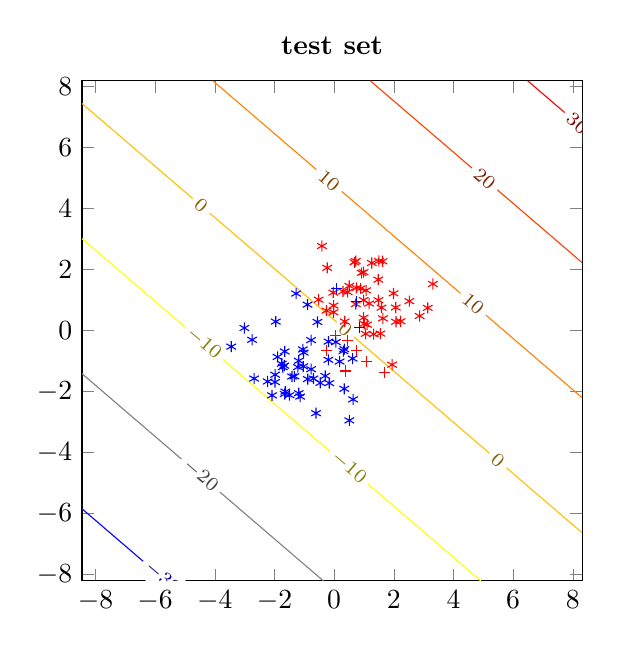
\begin{tikzpicture}

\begin{axis}[%
width=2.5in,
height=2.5in,
at={(0.668056in,0.48125in)},
scale only axis,
xmin=-8.44901775375681,
xmax=8.30928748595239,
ymin=-8.20232071732344,
ymax=8.1831858181971,
title style={font=\bfseries},
title={test set}
]
\addplot[contour prepared, contour prepared format=matlab] table[row sep=crcr] {%
%
-30	13\\
-8.44901775375681	-5.84210674080754\\
-8.13983713383397	-6.10161475123106\\
-8.01931761940529	-6.20277173647289\\
-7.63927642142127	-6.52175594444954\\
-7.58961748505378	-6.56343673213827\\
-7.15991735070226	-6.92410172780362\\
-7.13871570900852	-6.94189713766801\\
-6.73021721635074	-7.28476672346899\\
-6.63815499659581	-7.36203833088649\\
-6.30051708199922	-7.64543171913434\\
-6.13759428418306	-7.78217952410496\\
-5.8708169476477	-8.00609671479971\\
-5.63703357177034	-8.20232071732344\\
-20	36\\
-8.44901775375681	-1.41507109992078\\
-8.37158734590058	-1.48006162582783\\
-8.01931761940529	-1.77573609558611\\
-7.87102663348781	-1.90020281904631\\
-7.58961748505378	-2.13640109125149\\
-7.37046592107511	-2.32034401226478\\
-7.15991735070226	-2.49706608691685\\
-6.86990520866238	-2.74048520548326\\
-6.73021721635074	-2.8577310825822\\
-6.36934449624965	-3.16062639870173\\
-6.30051708199922	-3.21839607824757\\
-5.8708169476477	-3.57906107391293\\
-5.86878378383692	-3.58076759192021\\
-5.44111681329619	-3.93972606957828\\
-5.36822307142419	-4.00090878513868\\
-5.01141667894467	-4.30039106524364\\
-4.86766235901146	-4.42104997835716\\
-4.58171654459315	-4.66105606090901\\
-4.36710164659874	-4.84119117157563\\
-4.15201641024163	-5.02172105657436\\
-3.866540934186	-5.26133236479411\\
-3.72231627589012	-5.38238605223971\\
-3.36598022177329	-5.68147355801259\\
-3.2926161415386	-5.74305104790509\\
-2.86541950936056	-6.10161475123106\\
-2.86291600718708	-6.10371604357045\\
-2.43321587283556	-6.4643810392358\\
-2.36485879694783	-6.52175594444954\\
-2.00351573848404	-6.82504603490116\\
-1.86429808453508	-6.94189713766801\\
-1.57381560413253	-7.18571103056652\\
-1.36373737212237	-7.36203833088649\\
-1.14411546978101	-7.54637602623188\\
-0.863176659709634	-7.78217952410496\\
-0.714415335429489	-7.90704102189723\\
-0.362615947296917	-8.20232071732344\\
-10	59\\
-8.44901775375681	3.011964540966\\
-8.10277684555438	2.72135030635692\\
-8.01931761940529	2.65129954530068\\
-7.6022161331417	2.30120911313845\\
-7.58961748505378	2.29063454963528\\
-7.15991735070226	1.92996955396994\\
-7.10165542072894	1.88106791991997\\
-6.73021721635074	1.56930455830461\\
-6.60109470831619	1.46092672670149\\
-6.30051708199922	1.20863956263922\\
-6.10053399590349	1.04078553348302\\
-5.8708169476477	0.847974566973851\\
-5.59997328349077	0.620644340264543\\
-5.44111681329619	0.487309571308486\\
-5.09941257107805	0.200503147046068\\
-5.01141667894467	0.126644575643124\\
-4.59885185866533	-0.219638046172405\\
-4.58171654459315	-0.234020420022236\\
-4.15201641024163	-0.594685415687577\\
-4.09829114625258	-0.63977923939088\\
-3.72231627589012	-0.955350411352945\\
-3.59773043383986	-1.05992043260936\\
-3.2926161415386	-1.3160154070183\\
-3.09716972142713	-1.48006162582783\\
-2.86291600718708	-1.67668040268366\\
-2.5966090090144	-1.90020281904631\\
-2.43321587283556	-2.03734539834902\\
-2.09604829660166	-2.32034401226478\\
-2.00351573848404	-2.39801039401437\\
-1.59548758418894	-2.74048520548326\\
-1.57381560413253	-2.75867538967974\\
-1.14411546978101	-3.1193403853451\\
-1.09492687177621	-3.16062639870173\\
-0.714415335429489	-3.48000538101046\\
-0.594366159363481	-3.58076759192021\\
-0.284715201077971	-3.84067037667581\\
-0.0938054469507442	-4.00090878513868\\
0.144984933273545	-4.20133537234117\\
0.406755265461971	-4.42104997835716\\
0.574685067625063	-4.56200036800653\\
0.907315977874715	-4.84119117157563\\
1.00438520197658	-4.92266536367189\\
1.40787669028743	-5.26133236479411\\
1.4340853363281	-5.28333035933726\\
1.86378547067962	-5.64399535500261\\
1.90843740270016	-5.68147355801259\\
2.29348560503113	-6.00466035066798\\
2.4089981151129	-6.10161475123106\\
2.72318573938265	-6.36532534633332\\
2.90955882752562	-6.52175594444954\\
3.15288587373417	-6.72599034199867\\
3.41011953993836	-6.94189713766801\\
3.58258600808569	-7.08665533766405\\
3.91068025235107	-7.36203833088649\\
4.01228614243721	-7.44732033332941\\
4.4112409647638	-7.78217952410496\\
4.44198627678873	-7.80798532899478\\
4.87168641114024	-8.1686503246601\\
4.91180167717656	-8.20232071732344\\
0	74\\
-8.44901775375681	7.43900018185279\\
-8.33452705762097	7.34290343176015\\
-8.01931761940529	7.07833518618744\\
-7.83396634520824	6.92276223854167\\
-7.58961748505378	6.71767019052209\\
-7.3334056327955	6.5026210453232\\
-7.15991735070226	6.35700519485672\\
-6.83284492038282	6.08247985210472\\
-6.73021721635074	5.99634019919135\\
-6.33228420797006	5.66233865888625\\
-6.30051708199922	5.635675203526\\
-5.8708169476477	5.27501020786061\\
-5.83172349555736	5.24219746566777\\
-5.44111681329619	4.9143452121953\\
-5.33116278314459	4.8220562724493\\
-5.01141667894467	4.5536802165299\\
-4.8306020707319	4.40191507923082\\
-4.58171654459315	4.19301522086456\\
-4.33004135831917	3.98177388601235\\
-4.15201641024163	3.83235022519919\\
-3.82948064590645	3.56163269279387\\
-3.72231627589012	3.47168522953383\\
-3.32891993349368	3.1414914995754\\
-3.2926161415386	3.11102023386849\\
-2.86291600718708	2.75035523820311\\
-2.82835922108098	2.72135030635692\\
-2.43321587283556	2.38969024253775\\
-2.32779850866825	2.30120911313845\\
-2.00351573848404	2.0290252468724\\
-1.82723779625552	1.88106791991997\\
-1.57381560413253	1.66836025120704\\
-1.32667708384279	1.46092672670149\\
-1.14411546978101	1.30769525554168\\
-0.826116371430058	1.04078553348302\\
-0.714415335429489	0.947030259876319\\
-0.325555659017334	0.620644340264543\\
-0.284715201077971	0.586365264210958\\
0.144984933273545	0.2257002685456\\
0.175005053395395	0.200503147046068\\
0.574685067625063	-0.134964727119756\\
0.675565765808124	-0.219638046172405\\
1.00438520197658	-0.495629722785114\\
1.17612647822085	-0.63977923939088\\
1.4340853363281	-0.856294718450475\\
1.67668719063359	-1.05992043260936\\
1.86378547067962	-1.21695971411582\\
2.17724790304631	-1.48006162582783\\
2.29348560503113	-1.5776247097812\\
2.677808615459	-1.90020281904631\\
2.72318573938265	-1.93828970544658\\
3.15288587373417	-2.29895470111192\\
3.17836932787176	-2.32034401226478\\
3.58258600808569	-2.65961969677725\\
3.67893004028452	-2.74048520548326\\
4.01228614243721	-3.02028469244263\\
4.17949075269723	-3.16062639870173\\
4.44198627678873	-3.38094968810799\\
4.68005146510997	-3.58076759192021\\
4.87168641114024	-3.74161468377334\\
5.1806121775227	-4.00090878513868\\
5.30138654549176	-4.10227967943869\\
5.68117288993546	-4.42104997835716\\
5.73108667984328	-4.46294467510403\\
6.1607868141948	-4.8236096707694\\
6.18173360234818	-4.84119117157563\\
6.59048694854632	-5.18427466643483\\
6.68229431476083	-5.26133236479411\\
7.02018708289783	-5.54493966210017\\
7.18285502717357	-5.68147355801259\\
7.44988721724935	-5.90560465776552\\
7.68341573958635	-6.10161475123106\\
7.87958735160087	-6.26626965343084\\
8.18397645199912	-6.52175594444954\\
8.30928748595239	-6.62693464909617\\
10	54\\
-4.06123085797303	8.1831858181971\\
-3.72231627589012	7.89872087042061\\
-3.56067014556032	7.76304462497863\\
-3.2926161415386	7.53805587475521\\
-3.06010943314753	7.34290343176015\\
-2.86291600718708	7.17739087908991\\
-2.5595487207348	6.92276223854167\\
-2.43321587283556	6.81672588342456\\
-2.0589880083221	6.5026210453232\\
-2.00351573848404	6.45606088775917\\
-1.57381560413253	6.09539589209383\\
-1.55842729590936	6.08247985210472\\
-1.14411546978101	5.73473089642844\\
-1.05786658349666	5.66233865888625\\
-0.714415335429489	5.3740659007631\\
-0.55730587108391	5.24219746566777\\
-0.284715201077971	5.01340090509774\\
-0.056745158671195	4.8220562724493\\
0.144984933273545	4.65273590943237\\
0.443815553741529	4.40191507923082\\
0.574685067625063	4.29207091376701\\
0.944376266154268	3.98177388601235\\
1.00438520197658	3.93140591810165\\
1.4340853363281	3.57074092243632\\
1.44493697856702	3.56163269279387\\
1.86378547067962	3.21007592677094\\
1.94549769097973	3.1414914995754\\
2.29348560503113	2.84941093110558\\
2.44605840339246	2.72135030635692\\
2.72318573938265	2.48874593544022\\
2.94661911580519	2.30120911313845\\
3.15288587373417	2.12808093977487\\
3.44717982821792	1.88106791991997\\
3.58258600808569	1.76741594410951\\
3.94774054063063	1.46092672670149\\
4.01228614243721	1.40675094844413\\
4.44198627678873	1.04608595277879\\
4.44830125304338	1.04078553348302\\
4.87168641114024	0.685420957113439\\
4.94886196545612	0.620644340264543\\
5.30138654549176	0.324755961448065\\
5.44942267786883	0.200503147046068\\
5.73108667984328	-0.0359090342172951\\
5.94998339028156	-0.219638046172405\\
6.1607868141948	-0.396574029882647\\
6.45054410269429	-0.63977923939088\\
6.59048694854632	-0.757239025548003\\
6.951104815107	-1.05992043260936\\
7.02018708289783	-1.11790402121339\\
7.44988721724935	-1.4785690168787\\
7.45166552751978	-1.48006162582783\\
7.87958735160087	-1.83923401254405\\
7.95222623993251	-1.90020281904631\\
8.30928748595239	-2.19989900820942\\
20	32\\
1.21318676650038	8.1831858181971\\
1.4340853363281	7.99777656332306\\
1.71374747891317	7.76304462497863\\
1.86378547067962	7.63711156765774\\
2.21430819132587	7.34290343176015\\
2.29348560503113	7.27644657199235\\
2.71486890373858	6.92276223854167\\
2.72318573938265	6.91578157632698\\
3.15288587373417	6.55511658066165\\
3.21542961615135	6.5026210453232\\
3.58258600808569	6.19445158499629\\
3.71599032856408	6.08247985210472\\
4.01228614243721	5.83378658933093\\
4.2165510409768	5.66233865888625\\
4.44198627678873	5.47312159366556\\
4.71711175338952	5.24219746566777\\
4.87168641114024	5.1124565980002\\
5.21767246580226	4.8220562724493\\
5.30138654549176	4.75179160233485\\
5.71823317821498	4.40191507923082\\
5.73108667984328	4.39112660666948\\
6.1607868141948	4.03046161100413\\
6.21879389062772	3.98177388601235\\
6.59048694854632	3.66979661533877\\
6.71935460304045	3.56163269279387\\
7.02018708289783	3.30913161967342\\
7.21991531545317	3.1414914995754\\
7.44988721724935	2.94846662400805\\
7.72047602786589	2.72135030635692\\
7.87958735160087	2.58780162834267\\
8.22103674027862	2.30120911313845\\
8.30928748595239	2.22713663267733\\
30	9\\
6.48760439097385	8.1831858181971\\
6.59048694854632	8.09683225622554\\
6.98816510338661	7.76304462497863\\
7.02018708289783	7.7361672605602\\
7.44988721724935	7.37550226489482\\
7.48872581579931	7.34290343176015\\
7.87958735160087	7.01483726922946\\
7.98928652821204	6.92276223854167\\
8.30928748595239	6.65417227356411\\
};
\addplot [color=red,only marks,mark=asterisk,mark options={solid},forget plot]
  table[row sep=crcr]{%
1.63527413474712	0.398587873730275\\
};
\addplot [color=red,only marks,mark=asterisk,mark options={solid},forget plot]
  table[row sep=crcr]{%
1.5511847118249	-0.0998404547108134\\
};
\addplot [color=red,only marks,mark=+,mark options={solid},forget plot]
  table[row sep=crcr]{%
1.08599059329372	-1.00456332159079\\
};
\addplot [color=red,only marks,mark=asterisk,mark options={solid},forget plot]
  table[row sep=crcr]{%
0.506912082340303	1.46204801179919\\
};
\addplot [color=red,only marks,mark=asterisk,mark options={solid},forget plot]
  table[row sep=crcr]{%
0.678995307818708	2.23655565160192\\
};
\addplot [color=red,only marks,mark=+,mark options={solid},forget plot]
  table[row sep=crcr]{%
0.368720343274854	-1.32521112888377\\
};
\addplot [color=red,only marks,mark=asterisk,mark options={solid},forget plot]
  table[row sep=crcr]{%
-0.231636533325015	2.05564838790246\\
};
\addplot [color=red,only marks,mark=asterisk,mark options={solid},forget plot]
  table[row sep=crcr]{%
0.886776010630975	1.37922362268503\\
};
\addplot [color=red,only marks,mark=asterisk,mark options={solid},forget plot]
  table[row sep=crcr]{%
1.94419972674731	-1.12042668822421\\
};
\addplot [color=red,only marks,mark=asterisk,mark options={solid},forget plot]
  table[row sep=crcr]{%
0.355321084458063	0.295698271566391\\
};
\addplot [color=red,only marks,mark=asterisk,mark options={solid},forget plot]
  table[row sep=crcr]{%
-0.0181372163990707	0.817918131588615\\
};
\addplot [color=red,only marks,mark=asterisk,mark options={solid},forget plot]
  table[row sep=crcr]{%
2.52101323900559	0.961561236113288\\
};
\addplot [color=red,only marks,mark=asterisk,mark options={solid},forget plot]
  table[row sep=crcr]{%
2.22744798900972	0.303795199967111\\
};
\addplot [color=red,only marks,mark=asterisk,mark options={solid},forget plot]
  table[row sep=crcr]{%
1.00752448652301	0.217106955621713\\
};
\addplot [color=red,only marks,mark=asterisk,mark options={solid},forget plot]
  table[row sep=crcr]{%
1.58693855921443	0.748792625431118\\
};
\addplot [color=red,only marks,mark=asterisk,mark options={solid},forget plot]
  table[row sep=crcr]{%
1.4801358228426	1.66815503443364\\
};
\addplot [color=red,only marks,mark=asterisk,mark options={solid},forget plot]
  table[row sep=crcr]{%
0.921678803726588	1.8891726184126\\
};
\addplot [color=red,only marks,mark=asterisk,mark options={solid},forget plot]
  table[row sep=crcr]{%
3.30928748595239	1.5246386797711\\
};
\addplot [color=red,only marks,mark=asterisk,mark options={solid},forget plot]
  table[row sep=crcr]{%
0.988212676048693	1.91314081776137\\
};
\addplot [color=red,only marks,mark=asterisk,mark options={solid},forget plot]
  table[row sep=crcr]{%
1.0559406788884	-0.107069894826007\\
};
\addplot [color=red,only marks,mark=asterisk,mark options={solid},forget plot]
  table[row sep=crcr]{%
1.48549770731281	0.994994926244469\\
};
\addplot [color=red,only marks,mark=asterisk,mark options={solid},forget plot]
  table[row sep=crcr]{%
0.723782140645241	2.27645247367439\\
};
\addplot [color=red,only marks,mark=asterisk,mark options={solid},forget plot]
  table[row sep=crcr]{%
2.86340061318454	0.477440698363601\\
};
\addplot [color=red,only marks,mark=asterisk,mark options={solid},forget plot]
  table[row sep=crcr]{%
1.10342444693731	0.19235086910282\\
};
\addplot [color=red,only marks,mark=+,mark options={solid},forget plot]
  table[row sep=crcr]{%
1.68043858374895	-1.36458984794158\\
};
\addplot [color=red,only marks,mark=asterisk,mark options={solid},forget plot]
  table[row sep=crcr]{%
1.99011487204949	1.21889912088118\\
};
\addplot [color=red,only marks,mark=asterisk,mark options={solid},forget plot]
  table[row sep=crcr]{%
1.2616624601614	2.21344449497535\\
};
\addplot [color=red,only marks,mark=asterisk,mark options={solid},forget plot]
  table[row sep=crcr]{%
0.725333013543219	0.866865549186471\\
};
\addplot [color=red,only marks,mark=+,mark options={solid},forget plot]
  table[row sep=crcr]{%
-0.270500203708377	-0.663606452829772\\
};
\addplot [color=red,only marks,mark=asterisk,mark options={solid},forget plot]
  table[row sep=crcr]{%
0.296445738463245	1.2808804885233\\
};
\addplot [color=red,only marks,mark=+,mark options={solid},forget plot]
  table[row sep=crcr]{%
0.458790670083806	-0.333530729736393\\
};
\addplot [color=red,only marks,mark=asterisk,mark options={solid},forget plot]
  table[row sep=crcr]{%
2.07268626789014	0.287914547505644\\
};
\addplot [color=red,only marks,mark=asterisk,mark options={solid},forget plot]
  table[row sep=crcr]{%
0.988714438769314	0.999182970804304\\
};
\addplot [color=red,only marks,mark=asterisk,mark options={solid},forget plot]
  table[row sep=crcr]{%
0.750563715304566	1.39657531871165\\
};
\addplot [color=red,only marks,mark=+,mark options={solid},forget plot]
  table[row sep=crcr]{%
0.735986645077757	-0.664010876930589\\
};
\addplot [color=red,only marks,mark=asterisk,mark options={solid},forget plot]
  table[row sep=crcr]{%
-0.028975099543801	1.24309470022456\\
};
\addplot [color=red,only marks,mark=asterisk,mark options={solid},forget plot]
  table[row sep=crcr]{%
-0.256590107833817	0.652816810266474\\
};
\addplot [color=red,only marks,mark=+,mark options={solid},forget plot]
  table[row sep=crcr]{%
0.0586278065716714	-0.174560281302444\\
};
\addplot [color=red,only marks,mark=asterisk,mark options={solid},forget plot]
  table[row sep=crcr]{%
-0.021141686935775	0.598333265403212\\
};
\addplot [color=red,only marks,mark=asterisk,mark options={solid},forget plot]
  table[row sep=crcr]{%
1.17366566856231	0.883881506649489\\
};
\addplot [color=red,only marks,mark=asterisk,mark options={solid},forget plot]
  table[row sep=crcr]{%
2.06411914898635	0.75461370324833\\
};
\addplot [color=red,only marks,mark=asterisk,mark options={solid},forget plot]
  table[row sep=crcr]{%
-0.517539131089556	1.00973415912595\\
};
\addplot [color=red,only marks,mark=asterisk,mark options={solid},forget plot]
  table[row sep=crcr]{%
1.07137286485595	1.31653581376851\\
};
\addplot [color=red,only marks,mark=asterisk,mark options={solid},forget plot]
  table[row sep=crcr]{%
1.49982566779648	2.27808414671411\\
};
\addplot [color=red,only marks,mark=asterisk,mark options={solid},forget plot]
  table[row sep=crcr]{%
0.452183853078842	1.26080839887907\\
};
\addplot [color=red,only marks,mark=asterisk,mark options={solid},forget plot]
  table[row sep=crcr]{%
0.986823328126488	0.419735997858047\\
};
\addplot [color=red,only marks,mark=asterisk,mark options={solid},forget plot]
  table[row sep=crcr]{%
3.13630842280531	0.742382884346519\\
};
\addplot [color=red,only marks,mark=asterisk,mark options={solid},forget plot]
  table[row sep=crcr]{%
-0.409528489369198	2.77010089285161\\
};
\addplot [color=red,only marks,mark=asterisk,mark options={solid},forget plot]
  table[row sep=crcr]{%
1.32554598476071	-0.119039575381312\\
};
\addplot [color=red,only marks,mark=asterisk,mark options={solid},forget plot]
  table[row sep=crcr]{%
1.62035013944552	2.26978184718977\\
};
\addplot [color=blue,only marks,mark=asterisk,mark options={solid},forget plot]
  table[row sep=crcr]{%
-1.89604250642191	-0.864824555241563\\
};
\addplot [color=blue,only marks,mark=asterisk,mark options={solid},forget plot]
  table[row sep=crcr]{%
-1.13904001004044	-2.16339529383727\\
};
\addplot [color=blue,only marks,mark=asterisk,mark options={solid},forget plot]
  table[row sep=crcr]{%
0.183719539936857	-1.01542966178332\\
};
\addplot [color=blue,only marks,mark=asterisk,mark options={solid},forget plot]
  table[row sep=crcr]{%
-0.463781305281383	-1.71642862372586\\
};
\addplot [color=blue,only marks,mark=asterisk,mark options={solid},forget plot]
  table[row sep=crcr]{%
-1.65555938950391	-0.685637236689252\\
};
\addplot [color=blue,only marks,mark=asterisk,mark options={solid},forget plot]
  table[row sep=crcr]{%
-0.893185924065412	0.848216218018969\\
};
\addplot [color=blue,only marks,mark=asterisk,mark options={solid},forget plot]
  table[row sep=crcr]{%
-1.27510567543881	1.21255407898968\\
};
\addplot [color=blue,only marks,mark=asterisk,mark options={solid},forget plot]
  table[row sep=crcr]{%
0.508525756096147	-2.94507859991933\\
};
\addplot [color=blue,only marks,mark=asterisk,mark options={solid},forget plot]
  table[row sep=crcr]{%
-2.68054277752265	-1.57353413410588\\
};
\addplot [color=blue,only marks,mark=asterisk,mark options={solid},forget plot]
  table[row sep=crcr]{%
-1.18581652736766	-0.991065884323432\\
};
\addplot [color=blue,only marks,mark=asterisk,mark options={solid},forget plot]
  table[row sep=crcr]{%
-0.163050109162705	-1.7222706724333\\
};
\addplot [color=blue,only marks,mark=asterisk,mark options={solid},forget plot]
  table[row sep=crcr]{%
-1.72149047716441	-1.20118099951714\\
};
\addplot [color=blue,only marks,mark=asterisk,mark options={solid},forget plot]
  table[row sep=crcr]{%
-1.02046416109514	-0.721110000087549\\
};
\addplot [color=blue,only marks,mark=asterisk,mark options={solid},forget plot]
  table[row sep=crcr]{%
0.05829481445	-0.37832671759759\\
};
\addplot [color=blue,only marks,mark=asterisk,mark options={solid},forget plot]
  table[row sep=crcr]{%
-2.75061528848538	-0.302652448516563\\
};
\addplot [color=blue,only marks,mark=asterisk,mark options={solid},forget plot]
  table[row sep=crcr]{%
-0.188514136683007	-0.363655052395867\\
};
\addplot [color=blue,only marks,mark=asterisk,mark options={solid},forget plot]
  table[row sep=crcr]{%
0.310080341410262	-0.672902484081802\\
};
\addplot [color=blue,only marks,mark=asterisk,mark options={solid},forget plot]
  table[row sep=crcr]{%
-1.67299316385471	-1.14932749947673\\
};
\addplot [color=blue,only marks,mark=asterisk,mark options={solid},forget plot]
  table[row sep=crcr]{%
-3.44901775375681	-0.526714387756446\\
};
\addplot [color=blue,only marks,mark=asterisk,mark options={solid},forget plot]
  table[row sep=crcr]{%
-0.883054343206712	-1.5911038386322\\
};
\addplot [color=blue,only marks,mark=asterisk,mark options={solid},forget plot]
  table[row sep=crcr]{%
-1.65470767508278	-2.08066185121169\\
};
\addplot [color=blue,only marks,mark=asterisk,mark options={solid},forget plot]
  table[row sep=crcr]{%
-1.04773086529791	-0.620655462711205\\
};
\addplot [color=blue,only marks,mark=asterisk,mark options={solid},forget plot]
  table[row sep=crcr]{%
-1.33036104579866	-1.49989825118473\\
};
\addplot [color=blue,only marks,mark=asterisk,mark options={solid},forget plot]
  table[row sep=crcr]{%
-1.03597860795301	-1.17476033119672\\
};
\addplot [color=blue,only marks,mark=asterisk,mark options={solid},forget plot]
  table[row sep=crcr]{%
-1.95726507882166	0.292547900132268\\
};
\addplot [color=blue,only marks,mark=asterisk,mark options={solid},forget plot]
  table[row sep=crcr]{%
-0.559090357152978	0.280940942744541\\
};
\addplot [color=blue,only marks,mark=asterisk,mark options={solid},forget plot]
  table[row sep=crcr]{%
-1.49772980521188	-2.11871663760432\\
};
\addplot [color=blue,only marks,mark=asterisk,mark options={solid},forget plot]
  table[row sep=crcr]{%
-0.192350380560649	-0.958800421361755\\
};
\addplot [color=blue,only marks,mark=asterisk,mark options={solid},forget plot]
  table[row sep=crcr]{%
-1.7562086055467	-1.08912914780643\\
};
\addplot [color=blue,only marks,mark=asterisk,mark options={solid},forget plot]
  table[row sep=crcr]{%
-3.00885032178915	0.0839180379588267\\
};
\addplot [color=blue,only marks,mark=asterisk,mark options={solid},forget plot]
  table[row sep=crcr]{%
-1.98119056314417	-1.6884886374647\\
};
\addplot [color=blue,only marks,mark=asterisk,mark options={solid},forget plot]
  table[row sep=crcr]{%
0.339479481807799	-1.90924316031601\\
};
\addplot [color=blue,only marks,mark=asterisk,mark options={solid},forget plot]
  table[row sep=crcr]{%
-1.4128577286188	-1.50616318564854\\
};
\addplot [color=blue,only marks,mark=asterisk,mark options={solid},forget plot]
  table[row sep=crcr]{%
0.619747799125372	-0.9190992887935\\
};
\addplot [color=blue,only marks,mark=asterisk,mark options={solid},forget plot]
  table[row sep=crcr]{%
-2.08105649017694	-2.1245178115942\\
};
\addplot [color=blue,only marks,mark=+,mark options={solid},forget plot]
  table[row sep=crcr]{%
0.735676342606296	0.937458596526754\\
};
\addplot [color=blue,only marks,mark=asterisk,mark options={solid},forget plot]
  table[row sep=crcr]{%
0.635068218520641	-2.25594016677432\\
};
\addplot [color=blue,only marks,mark=asterisk,mark options={solid},forget plot]
  table[row sep=crcr]{%
-1.2135375062087	-1.19893204828268\\
};
\addplot [color=blue,only marks,mark=asterisk,mark options={solid},forget plot]
  table[row sep=crcr]{%
-0.692500822520151	-1.57232545648506\\
};
\addplot [color=blue,only marks,mark=asterisk,mark options={solid},forget plot]
  table[row sep=crcr]{%
-1.97764836704206	-1.44680940665695\\
};
\addplot [color=blue,only marks,mark=+,mark options={solid},forget plot]
  table[row sep=crcr]{%
0.0820919008951635	1.37264794938999\\
};
\addplot [color=blue,only marks,mark=asterisk,mark options={solid},forget plot]
  table[row sep=crcr]{%
-0.770711663895569	-1.26662313612389\\
};
\addplot [color=blue,only marks,mark=asterisk,mark options={solid},forget plot]
  table[row sep=crcr]{%
-0.2983278230806	-1.48759049128981\\
};
\addplot [color=blue,only marks,mark=+,mark options={solid},forget plot]
  table[row sep=crcr]{%
0.862479725319099	0.106851110391344\\
};
\addplot [color=blue,only marks,mark=asterisk,mark options={solid},forget plot]
  table[row sep=crcr]{%
-2.22756572221585	-1.66988511005649\\
};
\addplot [color=blue,only marks,mark=asterisk,mark options={solid},forget plot]
  table[row sep=crcr]{%
0.340929452331313	-0.611916683758858\\
};
\addplot [color=blue,only marks,mark=asterisk,mark options={solid},forget plot]
  table[row sep=crcr]{%
-0.606941071223	-2.70733357783774\\
};
\addplot [color=blue,only marks,mark=asterisk,mark options={solid},forget plot]
  table[row sep=crcr]{%
-0.772141355295662	-0.314367142237049\\
};
\addplot [color=blue,only marks,mark=asterisk,mark options={solid},forget plot]
  table[row sep=crcr]{%
-1.63679011291329	-2.00260555423381\\
};
\addplot [color=blue,only marks,mark=asterisk,mark options={solid},forget plot]
  table[row sep=crcr]{%
-1.18562067291102	-2.05403271420003\\
};
\end{axis}
\end{tikzpicture}%
\end{document}
% This file was created by matlab2tikz.
% Minimal pgfplots version: 1.3
%
%The latest updates can be retrieved from
%  http://www.mathworks.com/matlabcentral/fileexchange/22022-matlab2tikz
%where you can also make suggestions and rate matlab2tikz.
%
\documentclass[tikz]{standalone}
\usepackage{pgfplots}
\usepackage{grffile}
\pgfplotsset{compat=newest}
\usetikzlibrary{plotmarks}
\usepackage{amsmath}

\begin{document}
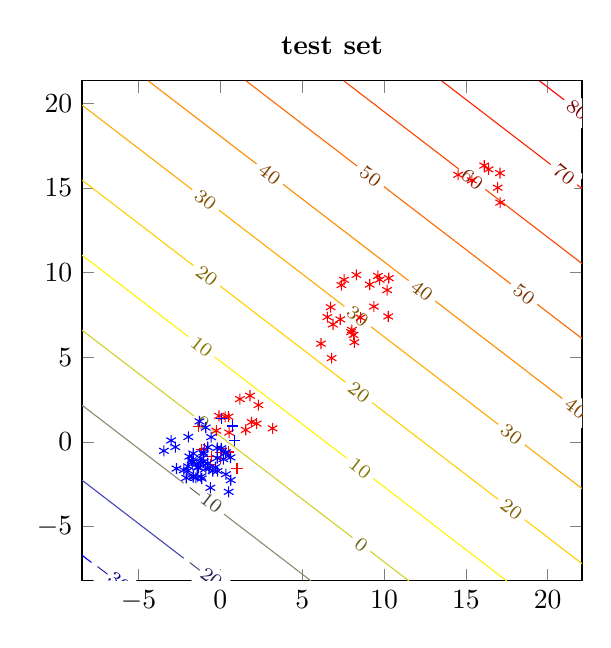
\begin{tikzpicture}

\begin{axis}[%
width=2.5in,
height=2.5in,
at={(0.668056in,0.48125in)},
scale only axis,
xmin=-8.44901775375681,
xmax=22.0950037387875,
ymin=-8.20232071732344,
ymax=21.3148090433951,
title style={font=\bfseries},
title={test set}
]
\addplot[contour prepared, contour prepared format=matlab] table[row sep=crcr] {%
%
-30	5\\
-8.44901775375681	-6.69077815523522\\
-7.66583771548645	-7.27132991834563\\
-7.43091636529865	-7.44547123627937\\
-6.88265767721608	-7.85188168145606\\
-6.40990593488808	-8.20232071732344\\
-20	19\\
-8.44901775375681	-2.261872924265\\
-7.66583771548645	-2.84242468737542\\
-7.58226594421673	-2.90437435001499\\
-6.88265767721608	-3.42297645048583\\
-6.56125551380612	-3.66122383105906\\
-6.09947763894571	-4.00352821359625\\
-5.54024508339555	-4.41807331210312\\
-5.31629760067535	-4.58407997670668\\
-4.53311756240498	-5.1646317398171\\
-4.51923465298496	-5.17492279314718\\
-3.74993752413461	-5.74518350292752\\
-3.49822422257436	-5.93177227419125\\
-2.96675748586425	-6.32573526603793\\
-2.47721379216376	-6.68862175523531\\
-2.18357744759388	-6.90628702914834\\
-1.45620336175319	-7.44547123627937\\
-1.40039740932351	-7.48683879225879\\
-0.617217371053146	-8.06739055536921\\
-0.435192931342599	-8.20232071732344\\
-10	32\\
-8.44901775375681	2.16703230670524\\
-7.73361552313474	1.63672253624939\\
-7.66583771548645	1.58648054359484\\
-6.88265767721608	1.0059287804844\\
-6.71260509272417	0.879873055205328\\
-6.09947763894571	0.42537701737397\\
-5.69159466231359	0.123023574161264\\
-5.31629760067535	-0.155174745736444\\
-4.670584231903	-0.633825906882799\\
-4.53311756240498	-0.735726508846872\\
-3.74993752413461	-1.3162782719573\\
-3.64957380149242	-1.39067538792686\\
-2.96675748586425	-1.89683003506772\\
-2.62856337108183	-2.14752486897093\\
-2.18357744759388	-2.47738179817813\\
-1.60755294067124	-2.90437435001499\\
-1.40039740932351	-3.05793356128855\\
-0.617217371053146	-3.63848532439898\\
-0.586542510260652	-3.66122383105906\\
0.165962667217221	-4.2190370875094\\
0.434467920149933	-4.41807331210312\\
0.949142705487589	-4.79958885061983\\
1.45547835056052	-5.17492279314718\\
1.73232274375795	-5.38014061373025\\
2.47648878097114	-5.93177227419125\\
2.51550278202832	-5.96069237684064\\
3.29868282029869	-6.54124413995108\\
3.4974992113817	-6.68862175523531\\
4.08186285856906	-7.12179590306151\\
4.5185096417923	-7.44547123627937\\
4.86504289683942	-7.70234766617192\\
5.5395200722029	-8.20232071732344\\
0	46\\
-8.44901775375681	6.59593753767546\\
-7.88496510205284	6.17781942251378\\
-7.66583771548645	6.01538577456503\\
-6.88265767721608	5.43483401145461\\
-6.86395467164225	5.42096994146971\\
-6.09947763894571	4.8542822483442\\
-5.84294424123164	4.66412046042565\\
-5.31629760067535	4.27373048523377\\
-4.82193381082106	3.90727097938158\\
-4.53311756240498	3.69317872212335\\
-3.80092338041047	3.15042149833752\\
-3.74993752413461	3.11262695901293\\
-2.96675748586425	2.53207519590251\\
-2.77991294999988	2.39357201729346\\
-2.18357744759388	1.95152343279209\\
-1.75890251958929	1.63672253624939\\
-1.40039740932351	1.37097166968167\\
-0.737892089178704	0.879873055205328\\
-0.617217371053146	0.790419906571245\\
0.165962667217221	0.209868143460825\\
0.283118341231886	0.123023574161264\\
0.949142705487589	-0.370683619649598\\
1.30412877164247	-0.633825906882799\\
1.73232274375795	-0.951235382760018\\
2.32513920205306	-1.39067538792686\\
2.51550278202832	-1.53178714587044\\
3.29868282029869	-2.11233890898086\\
3.34614963246365	-2.14752486897093\\
4.08186285856906	-2.69289067209127\\
4.36716006287425	-2.90437435001499\\
4.86504289683942	-3.27344243520169\\
5.38817049328483	-3.66122383105906\\
5.64822293510979	-3.85399419831213\\
6.40918092369539	-4.41807331210312\\
6.43140297338016	-4.43454596142256\\
7.21458301165052	-5.01509772453297\\
7.430191354106	-5.17492279314718\\
7.99776304992089	-5.59564948764338\\
8.4512017845166	-5.93177227419125\\
8.78094308819126	-6.17620125075381\\
9.4722122149272	-6.68862175523531\\
9.56412312646162	-6.75675301386422\\
10.347303164732	-7.33730477697461\\
10.4932226453378	-7.44547123627937\\
11.1304832030024	-7.91785654008508\\
11.5142330757484	-8.20232071732344\\
10	60\\
-8.44901775375681	11.0248427686457\\
-8.03631468097088	10.7189163087782\\
-7.66583771548645	10.4442910055353\\
-7.01530425056029	9.9620668277341\\
-6.88265767721608	9.86373924242484\\
-6.09947763894571	9.28318747931442\\
-5.9942938201497	9.20521734669003\\
-5.31629760067535	8.70263571620399\\
-4.97328338973912	8.44836786564597\\
-4.53311756240498	8.12208395309356\\
-3.95227295932853	7.6915183846019\\
-3.74993752413461	7.54153218998315\\
-2.96675748586425	6.96098042687272\\
-2.93126252891795	6.93466890355784\\
-2.18357744759388	6.38042866376231\\
-1.91025209850735	6.17781942251378\\
-1.40039740932351	5.79987690065189\\
-0.889241668096753	5.42096994146971\\
-0.617217371053146	5.21932513754146\\
0.131768762313821	4.66412046042565\\
0.165962667217221	4.63877337443104\\
0.949142705487589	4.05822161132062\\
1.15277919272442	3.90727097938158\\
1.73232274375795	3.47766984821021\\
2.17378962313501	3.15042149833752\\
2.51550278202832	2.89711808509978\\
3.19480005354559	2.39357201729346\\
3.29868282029869	2.31656632198935\\
4.08186285856906	1.73601455887895\\
4.2158104839562	1.63672253624939\\
4.86504289683942	1.15546279576853\\
5.23682091436678	0.879873055205328\\
5.64822293510979	0.574911032658096\\
6.25783134477737	0.123023574161264\\
6.43140297338016	-0.00564073045231372\\
7.21458301165052	-0.586192493562759\\
7.27884177518793	-0.633825906882799\\
7.99776304992089	-1.16674425667315\\
8.29985220559854	-1.39067538792686\\
8.78094308819126	-1.74729601978358\\
9.32086263600915	-2.14752486897093\\
9.56412312646162	-2.32784778289399\\
10.3418730664197	-2.90437435001499\\
10.347303164732	-2.90839954600444\\
11.1304832030024	-3.48895130911487\\
11.3628834968303	-3.66122383105906\\
11.9136632412727	-4.06950307222525\\
12.3838939272409	-4.41807331210312\\
12.6968432795431	-4.65005483533568\\
13.4049043576515	-5.17492279314718\\
13.4800233178135	-5.23060659844608\\
14.2632033560838	-5.81115836155652\\
14.4259147880621	-5.93177227419125\\
15.0463833943542	-6.39171012466694\\
15.4469252184727	-6.68862175523531\\
15.8295634326246	-6.97226188777737\\
16.4679356488833	-7.44547123627937\\
16.6127434708949	-7.55281365088777\\
17.3959235091653	-8.13336541399824\\
17.4889460792938	-8.20232071732344\\
20	70\\
-8.44901775375681	15.4537479996159\\
-8.18766425988888	15.2600131950425\\
-7.66583771548645	14.8731962365055\\
-7.16665382947838	14.5031637139985\\
-6.88265767721608	14.292644473395\\
-6.14564339906775	13.7463142329544\\
-6.09947763894571	13.7120927102846\\
-5.31629760067535	13.1315409471742\\
-5.12463296865717	12.9894647519104\\
-4.53311756240498	12.5509891840638\\
-4.10362253824658	12.2326152708663\\
-3.74993752413461	11.9704374209534\\
-3.08261210783597	11.4757657898222\\
-2.96675748586425	11.389885657843\\
-2.18357744759388	10.8093338947325\\
-2.06160167742539	10.7189163087782\\
-1.40039740932351	10.2287821316221\\
-1.04059124701481	9.9620668277341\\
-0.617217371053146	9.6482303685117\\
-0.0195808166042212	9.20521734669003\\
0.165962667217221	9.06767860540127\\
0.949142705487589	8.48712684229085\\
1.00142961380637	8.44836786564597\\
1.73232274375795	7.90657507918044\\
2.02244004421697	7.6915183846019\\
2.51550278202832	7.32602331607001\\
3.04345047462755	6.93466890355784\\
3.29868282029869	6.7454715529596\\
4.06446090503816	6.17781942251378\\
4.08186285856906	6.16491978984918\\
4.86504289683942	5.58436802673875\\
5.08547133544872	5.42096994146971\\
5.64822293510979	5.00381626362833\\
6.10648176585931	4.66412046042565\\
6.43140297338016	4.4232645005179\\
7.12749219626989	3.90727097938158\\
7.21458301165052	3.84271273740748\\
7.99776304992089	3.26216097429704\\
8.14850262668046	3.15042149833752\\
8.78094308819126	2.68160921118662\\
9.16951305709105	2.39357201729346\\
9.56412312646162	2.1010574480762\\
10.1905234875017	1.63672253624939\\
10.347303164732	1.52050568496579\\
11.1304832030024	0.939953921855371\\
11.2115339179123	0.879873055205328\\
11.9136632412727	0.359402158744985\\
12.2325443483229	0.123023574161264\\
12.6968432795431	-0.221149604365461\\
13.2535547787334	-0.633825906882799\\
13.4800233178135	-0.80170136747589\\
14.2632033560838	-1.38225313058633\\
14.274565209144	-1.39067538792686\\
15.0463833943542	-1.96280489369671\\
15.2955756395546	-2.14752486897093\\
15.8295634326246	-2.54335665680713\\
16.3165860699652	-2.90437435001499\\
16.6127434708949	-3.12390841991758\\
17.3375965003759	-3.66122383105906\\
17.3959235091653	-3.70446018302793\\
18.1791035474357	-4.28501194613839\\
18.3586069307864	-4.41807331210312\\
18.962283585706	-4.86556370924883\\
19.3796173611969	-5.17492279314718\\
19.7454636239764	-5.44611547235932\\
20.4006277916075	-5.93177227419125\\
20.5286436622468	-6.0266672354697\\
21.3118237005171	-6.60721899858007\\
21.4216382220182	-6.68862175523531\\
22.0950037387875	-7.18777076169053\\
30	70\\
-8.44901775375681	19.8826532305861\\
-8.33901383880697	19.8011100813069\\
-7.66583771548645	19.3021014674757\\
-7.31800340839641	19.0442606002629\\
-6.88265767721608	18.7215497043653\\
-6.29699297798578	18.2874111192188\\
-6.09947763894571	18.1409979412549\\
-5.31629760067535	17.5604461781444\\
-5.27598254757525	17.5305616381747\\
-4.53311756240498	16.979894415034\\
-4.25497211716461	16.7737121571307\\
-3.74993752413461	16.3993426519236\\
-3.23396168675404	16.0168626760866\\
-2.96675748586425	15.8187908888132\\
-2.21295125634341	15.2600131950425\\
-2.18357744759388	15.2382391257028\\
-1.40039740932351	14.6576873625924\\
-1.19194082593284	14.5031637139985\\
-0.617217371053146	14.0771355994819\\
-0.170930395522275	13.7463142329544\\
0.165962667217221	13.4965838363715\\
0.850080034888325	12.9894647519104\\
0.949142705487589	12.9160320732611\\
1.73232274375795	12.3354803101507\\
1.8710904652989	12.2326152708663\\
2.51550278202832	11.7549285470403\\
2.8921008957095	11.4757657898222\\
3.29868282029869	11.1743767839298\\
3.91311132612007	10.7189163087782\\
4.08186285856906	10.5938250208194\\
4.86504289683942	10.013273257709\\
4.93412175653067	9.9620668277341\\
5.64822293510979	9.43272149459855\\
5.95513218694125	9.20521734669003\\
6.43140297338016	8.85216973148812\\
6.97614261735185	8.44836786564597\\
7.21458301165052	8.27161796837771\\
7.99715304776245	7.6915183846019\\
7.99776304992089	7.6910662052673\\
8.78094308819126	7.11051444215684\\
9.018163478173	6.93466890355784\\
9.56412312646162	6.52996267904644\\
10.0391739085836	6.17781942251378\\
10.347303164732	5.94941091593603\\
11.0601843389943	5.42096994146971\\
11.1304832030024	5.36885915282564\\
11.9136632412727	4.78830738971518\\
12.0811947694048	4.66412046042565\\
12.6968432795431	4.20775562660479\\
13.1022051998154	3.90727097938158\\
13.4800233178135	3.62720386349436\\
14.123215630226	3.15042149833752\\
14.2632033560838	3.04665210038392\\
15.0463833943542	2.46610033727351\\
15.1442260606366	2.39357201729346\\
15.8295634326246	1.88554857416309\\
16.1652364910472	1.63672253624939\\
16.6127434708949	1.30499681105268\\
17.1862469214577	0.879873055205328\\
17.3959235091653	0.724445047942197\\
18.1791035474357	0.143893284831826\\
18.2072573518683	0.123023574161264\\
18.962283585706	-0.436658478278624\\
19.2282677822789	-0.633825906882799\\
19.7454636239764	-1.017210241389\\
20.2492782126895	-1.39067538792686\\
20.5286436622468	-1.59776200449946\\
21.2702886431001	-2.14752486897093\\
21.3118237005171	-2.17831376760984\\
22.0950037387875	-2.75886553072035\\
40	60\\
-4.40632169608275	21.3148090433951\\
-3.74993752413461	20.8282478828938\\
-3.38531126567218	20.557959562351\\
-2.96675748586425	20.2476961197834\\
-2.36430083526152	19.8011100813069\\
-2.18357744759388	19.667144356673\\
-1.40039740932351	19.0865925935625\\
-1.34329040485094	19.0442606002629\\
-0.617217371053146	18.5060408304521\\
-0.322279974440309	18.2874111192188\\
0.165962667217221	17.9254890673417\\
0.698730455970253	17.5305616381747\\
0.949142705487589	17.3449373042313\\
1.71974088638085	16.7737121571307\\
1.73232274375795	16.7643855411209\\
2.51550278202832	16.1838337780104\\
2.74075131679143	16.0168626760866\\
3.29868282029869	15.6032820149001\\
3.76176174720205	15.2600131950425\\
4.08186285856906	15.0227302517896\\
4.78277217761265	14.5031637139985\\
4.86504289683942	14.4421784886792\\
5.64822293510979	13.8616267255688\\
5.8037826080232	13.7463142329544\\
6.43140297338016	13.2810749624584\\
6.82479303843381	12.9894647519104\\
7.21458301165052	12.7005231993479\\
7.84580346884439	12.2326152708663\\
7.99776304992089	12.1199714362375\\
8.78094308819126	11.5394196731271\\
8.866813899255	11.4757657898222\\
9.56412312646162	10.9588679100167\\
9.88782432966554	10.7189163087782\\
10.347303164732	10.3783161469062\\
10.9088347600761	9.9620668277341\\
11.1304832030024	9.7977643837958\\
11.9136632412727	9.2172126206854\\
11.9298451904867	9.20521734669003\\
12.6968432795431	8.636660857575\\
12.9508556208973	8.44836786564597\\
13.4800233178135	8.05610909446457\\
13.9718660513079	7.6915183846019\\
14.2632033560838	7.47555733135413\\
14.9928764817186	6.93466890355784\\
15.0463833943542	6.89500556824376\\
15.8295634326246	6.31445380513327\\
16.013886912129	6.17781942251378\\
16.6127434708949	5.73390204202288\\
17.0348973425397	5.42096994146971\\
17.3959235091653	5.15335027891248\\
18.0559077729503	4.66412046042565\\
18.1791035474357	4.57279851580203\\
18.962283585706	3.99224675269163\\
19.0769182033609	3.90727097938158\\
19.7454636239764	3.41169498958116\\
20.0979286337714	3.15042149833752\\
20.5286436622468	2.8311432264708\\
21.118939064182	2.39357201729346\\
21.3118237005171	2.25059146336035\\
22.0950037387875	1.67003970024992\\
50	48\\
1.56839130746274	21.3148090433951\\
1.73232274375795	21.1932907720911\\
2.51550278202832	20.6127390089807\\
2.58940173787338	20.557959562351\\
3.29868282029869	20.0321872458703\\
3.61041216828396	19.8011100813069\\
4.08186285856906	19.4516354827598\\
4.63142259869459	19.0442606002629\\
4.86504289683942	18.8710837196494\\
5.64822293510979	18.290531956539\\
5.65243302910516	18.2874111192188\\
6.43140297338016	17.7099801934286\\
6.67344345951572	17.5305616381747\\
7.21458301165052	17.1294284303181\\
7.69445388992631	16.7737121571307\\
7.99776304992089	16.5488766672077\\
8.71546432033694	16.0168626760866\\
8.78094308819126	15.9683249040973\\
9.56412312646162	15.3877731409869\\
9.73647475074751	15.2600131950425\\
10.347303164732	14.8072213778765\\
10.7574851811581	14.5031637139985\\
11.1304832030024	14.2266696147661\\
11.7784956115687	13.7463142329544\\
11.9136632412727	13.6461178516556\\
12.6968432795431	13.0655660885452\\
12.7995060419793	12.9894647519104\\
13.4800233178135	12.4850143254348\\
13.8205164723899	12.2326152708663\\
14.2632033560838	11.9044625623244\\
14.8415269028004	11.4757657898222\\
15.0463833943542	11.3239107992139\\
15.8295634326246	10.7433590361035\\
15.8625373332111	10.7189163087782\\
16.6127434708949	10.1628072729931\\
16.8835477636217	9.9620668277341\\
17.3959235091653	9.58225550988269\\
17.9045581940322	9.20521734669003\\
18.1791035474357	9.00170374677227\\
18.9255686244428	8.44836786564597\\
18.962283585706	8.42115198366183\\
19.7454636239764	7.8406002205514\\
19.9465790548534	7.6915183846019\\
20.5286436622468	7.26004845744096\\
20.967589485264	6.93466890355784\\
21.3118237005171	6.67949669433061\\
21.9885999156746	6.17781942251378\\
22.0950037387875	6.09894493122016\\
60	34\\
7.54310431100827	21.3148090433951\\
7.99776304992089	20.977781898178\\
8.56411474141886	20.557959562351\\
8.78094308819126	20.3972301350675\\
9.56412312646162	19.8166783719571\\
9.58512517182947	19.8011100813069\\
10.347303164732	19.2361266088467\\
10.6061356022401	19.0442606002629\\
11.1304832030024	18.6555748457363\\
11.6271460326506	18.2874111192188\\
11.9136632412727	18.0750230826258\\
12.6481564630612	17.5305616381747\\
12.6968432795431	17.4944713195154\\
13.4800233178135	16.913919556405\\
13.6691668934718	16.7737121571307\\
14.2632033560838	16.3333677932946\\
14.6901773238824	16.0168626760866\\
15.0463833943542	15.7528160301842\\
15.711187754293	15.2600131950425\\
15.8295634326246	15.1722642670738\\
16.6127434708949	14.5917125039633\\
16.7321981847035	14.5031637139985\\
17.3959235091653	14.0111607408529\\
17.7532086151142	13.7463142329544\\
18.1791035474357	13.4306089777425\\
18.7742190455248	12.9894647519104\\
18.962283585706	12.8500572146321\\
19.7454636239764	12.2695054515217\\
19.7952294759354	12.2326152708663\\
20.5286436622468	11.6889536884112\\
20.8162399063459	11.4757657898222\\
21.3118237005171	11.1084019253008\\
21.8372503367565	10.7189163087782\\
22.0950037387875	10.5278501621903\\
70	20\\
13.5178173145538	21.3148090433951\\
14.2632033560838	20.7622730242648\\
14.5388277449643	20.557959562351\\
15.0463833943542	20.1817212611544\\
15.559838175375	19.8011100813069\\
15.8295634326246	19.601169498044\\
16.5808486057855	19.0442606002629\\
16.6127434708949	19.0206177349336\\
17.3959235091653	18.4400659718231\\
17.6018590361961	18.2874111192188\\
18.1791035474357	17.8595142087127\\
18.6228694666067	17.5305616381747\\
18.962283585706	17.2789624456023\\
19.6438798970172	16.7737121571307\\
19.7454636239764	16.6984106824918\\
20.5286436622468	16.1178589193815\\
20.6648903274279	16.0168626760866\\
21.3118237005171	15.537307156271\\
21.6859007578385	15.2600131950425\\
22.0950037387875	14.9567553931606\\
80	7\\
19.4925303180992	21.3148090433951\\
19.7454636239764	21.1273159134621\\
20.5135407485099	20.557959562351\\
20.5286436622468	20.5467641503517\\
21.3118237005171	19.9662123872413\\
21.5345511789204	19.8011100813069\\
22.0950037387875	19.3856606241308\\
};
\addplot [color=red,only marks,mark=asterisk,mark options={solid},forget plot]
  table[row sep=crcr]{%
-0.2463365280849	0.663024145855908\\
};
\addplot [color=red,only marks,mark=+,mark options={solid},forget plot]
  table[row sep=crcr]{%
0.0558011901764726	-0.367873566740638\\
};
\addplot [color=red,only marks,mark=asterisk,mark options={solid},forget plot]
  table[row sep=crcr]{%
9.62323385113849	9.79904861814778\\
};
\addplot [color=red,only marks,mark=asterisk,mark options={solid},forget plot]
  table[row sep=crcr]{%
-0.0793302230234205	1.53515226612215\\
};
\addplot [color=red,only marks,mark=asterisk,mark options={solid},forget plot]
  table[row sep=crcr]{%
0.535397954249106	0.552883517423822\\
};
\addplot [color=red,only marks,mark=asterisk,mark options={solid},forget plot]
  table[row sep=crcr]{%
9.38033725171391	7.99088447565921\\
};
\addplot [color=red,only marks,mark=+,mark options={solid},forget plot]
  table[row sep=crcr]{%
0.0112448963841337	-0.64514581569117\\
};
\addplot [color=red,only marks,mark=asterisk,mark options={solid},forget plot]
  table[row sep=crcr]{%
9.73095733842945	9.5778573463308\\
};
\addplot [color=red,only marks,mark=asterisk,mark options={solid},forget plot]
  table[row sep=crcr]{%
3.19083807424337	0.797542885226056\\
};
\addplot [color=red,only marks,mark=asterisk,mark options={solid},forget plot]
  table[row sep=crcr]{%
2.21932067266762	1.07809837564446\\
};
\addplot [color=red,only marks,mark=asterisk,mark options={solid},forget plot]
  table[row sep=crcr]{%
2.32729236140865	2.17463914282092\\
};
\addplot [color=red,only marks,mark=+,mark options={solid},forget plot]
  table[row sep=crcr]{%
-0.606482859277266	-1.34736267385024\\
};
\addplot [color=red,only marks,mark=asterisk,mark options={solid},forget plot]
  table[row sep=crcr]{%
0.497769664182782	1.48849047090348\\
};
\addplot [color=red,only marks,mark=+,mark options={solid},forget plot]
  table[row sep=crcr]{%
-1.31943699810954	0.931217514995436\\
};
\addplot [color=red,only marks,mark=+,mark options={solid},forget plot]
  table[row sep=crcr]{%
0.485295555916544	-0.595490902619476\\
};
\addplot [color=red,only marks,mark=+,mark options={solid},forget plot]
  table[row sep=crcr]{%
-0.546475894767623	-0.846758163883059\\
};
\addplot [color=red,only marks,mark=asterisk,mark options={solid},forget plot]
  table[row sep=crcr]{%
1.19490959580312	2.52874301096222\\
};
\addplot [color=red,only marks,mark=+,mark options={solid},forget plot]
  table[row sep=crcr]{%
-0.947146064738541	-0.374429195029166\\
};
\addplot [color=red,only marks,mark=+,mark options={solid},forget plot]
  table[row sep=crcr]{%
0.0214661388790944	-1.00394446674772\\
};
\addplot [color=red,only marks,mark=+,mark options={solid},forget plot]
  table[row sep=crcr]{%
-1.16781936472664	-0.460605179506151\\
};
\addplot [color=red,only marks,mark=asterisk,mark options={solid},forget plot]
  table[row sep=crcr]{%
1.90435159451633	1.16765053634998\\
};
\addplot [color=red,only marks,mark=asterisk,mark options={solid},forget plot]
  table[row sep=crcr]{%
0.289502034538413	1.47891705768128\\
};
\addplot [color=red,only marks,mark=asterisk,mark options={solid},forget plot]
  table[row sep=crcr]{%
1.81329142231856	2.7257905482933\\
};
\addplot [color=red,only marks,mark=+,mark options={solid},forget plot]
  table[row sep=crcr]{%
1.01841178862471	-1.58040249930316\\
};
\addplot [color=red,only marks,mark=asterisk,mark options={solid},forget plot]
  table[row sep=crcr]{%
1.55324256851535	0.707893884632476\\
};
\addplot [color=red,only marks,mark=asterisk,mark options={solid},forget plot]
  table[row sep=crcr]{%
8.1902449362512	5.88379124221439\\
};
\addplot [color=red,only marks,mark=asterisk,mark options={solid},forget plot]
  table[row sep=crcr]{%
10.2902497549325	9.66860050568204\\
};
\addplot [color=red,only marks,mark=asterisk,mark options={solid},forget plot]
  table[row sep=crcr]{%
15.3645347745207	15.4404266978038\\
};
\addplot [color=red,only marks,mark=asterisk,mark options={solid},forget plot]
  table[row sep=crcr]{%
16.1184448370541	16.3148090433951\\
};
\addplot [color=red,only marks,mark=asterisk,mark options={solid},forget plot]
  table[row sep=crcr]{%
16.9408899407278	15.0079082644562\\
};
\addplot [color=red,only marks,mark=asterisk,mark options={solid},forget plot]
  table[row sep=crcr]{%
8.03783419871876	6.61020045152317\\
};
\addplot [color=red,only marks,mark=asterisk,mark options={solid},forget plot]
  table[row sep=crcr]{%
6.53502663282888	7.37096058384895\\
};
\addplot [color=red,only marks,mark=asterisk,mark options={solid},forget plot]
  table[row sep=crcr]{%
10.1891642016521	8.96236672340668\\
};
\addplot [color=red,only marks,mark=asterisk,mark options={solid},forget plot]
  table[row sep=crcr]{%
7.39591443799884	9.25730423467749\\
};
\addplot [color=red,only marks,mark=asterisk,mark options={solid},forget plot]
  table[row sep=crcr]{%
8.30822429829771	9.85799667282826\\
};
\addplot [color=red,only marks,mark=asterisk,mark options={solid},forget plot]
  table[row sep=crcr]{%
8.13802801285837	6.31586141486366\\
};
\addplot [color=red,only marks,mark=asterisk,mark options={solid},forget plot]
  table[row sep=crcr]{%
6.14580262553102	5.79868518466096\\
};
\addplot [color=red,only marks,mark=asterisk,mark options={solid},forget plot]
  table[row sep=crcr]{%
7.32736756408083	7.23405701284718\\
};
\addplot [color=red,only marks,mark=asterisk,mark options={solid},forget plot]
  table[row sep=crcr]{%
14.5248654941447	15.765995952344\\
};
\addplot [color=red,only marks,mark=asterisk,mark options={solid},forget plot]
  table[row sep=crcr]{%
7.98633739100202	6.48136493365525\\
};
\addplot [color=red,only marks,mark=asterisk,mark options={solid},forget plot]
  table[row sep=crcr]{%
17.0822949531553	15.8685002970547\\
};
\addplot [color=red,only marks,mark=asterisk,mark options={solid},forget plot]
  table[row sep=crcr]{%
8.56743518847178	7.3344156217619\\
};
\addplot [color=red,only marks,mark=asterisk,mark options={solid},forget plot]
  table[row sep=crcr]{%
6.88013057194261	6.93470598515841\\
};
\addplot [color=red,only marks,mark=asterisk,mark options={solid},forget plot]
  table[row sep=crcr]{%
6.79630952043264	4.94567531944339\\
};
\addplot [color=red,only marks,mark=asterisk,mark options={solid},forget plot]
  table[row sep=crcr]{%
7.55903556809898	9.57114762365818\\
};
\addplot [color=red,only marks,mark=asterisk,mark options={solid},forget plot]
  table[row sep=crcr]{%
16.389880489687	16.0879871065798\\
};
\addplot [color=red,only marks,mark=asterisk,mark options={solid},forget plot]
  table[row sep=crcr]{%
9.12533230647483	9.28767642035855\\
};
\addplot [color=red,only marks,mark=asterisk,mark options={solid},forget plot]
  table[row sep=crcr]{%
10.2540014216025	7.40627042355252\\
};
\addplot [color=red,only marks,mark=asterisk,mark options={solid},forget plot]
  table[row sep=crcr]{%
17.0950037387875	14.126009742359\\
};
\addplot [color=red,only marks,mark=asterisk,mark options={solid},forget plot]
  table[row sep=crcr]{%
6.73889837693838	7.95346544550482\\
};
\addplot [color=blue,only marks,mark=asterisk,mark options={solid},forget plot]
  table[row sep=crcr]{%
-1.89604250642191	-0.864824555241563\\
};
\addplot [color=blue,only marks,mark=asterisk,mark options={solid},forget plot]
  table[row sep=crcr]{%
-1.13904001004044	-2.16339529383727\\
};
\addplot [color=blue,only marks,mark=asterisk,mark options={solid},forget plot]
  table[row sep=crcr]{%
0.183719539936857	-1.01542966178332\\
};
\addplot [color=blue,only marks,mark=asterisk,mark options={solid},forget plot]
  table[row sep=crcr]{%
-0.463781305281383	-1.71642862372586\\
};
\addplot [color=blue,only marks,mark=asterisk,mark options={solid},forget plot]
  table[row sep=crcr]{%
-1.65555938950391	-0.685637236689252\\
};
\addplot [color=blue,only marks,mark=asterisk,mark options={solid},forget plot]
  table[row sep=crcr]{%
-0.893185924065412	0.848216218018969\\
};
\addplot [color=blue,only marks,mark=asterisk,mark options={solid},forget plot]
  table[row sep=crcr]{%
-1.27510567543881	1.21255407898968\\
};
\addplot [color=blue,only marks,mark=asterisk,mark options={solid},forget plot]
  table[row sep=crcr]{%
0.508525756096147	-2.94507859991933\\
};
\addplot [color=blue,only marks,mark=asterisk,mark options={solid},forget plot]
  table[row sep=crcr]{%
-2.68054277752265	-1.57353413410588\\
};
\addplot [color=blue,only marks,mark=asterisk,mark options={solid},forget plot]
  table[row sep=crcr]{%
-1.18581652736766	-0.991065884323432\\
};
\addplot [color=blue,only marks,mark=asterisk,mark options={solid},forget plot]
  table[row sep=crcr]{%
-0.163050109162705	-1.7222706724333\\
};
\addplot [color=blue,only marks,mark=asterisk,mark options={solid},forget plot]
  table[row sep=crcr]{%
-1.72149047716441	-1.20118099951714\\
};
\addplot [color=blue,only marks,mark=asterisk,mark options={solid},forget plot]
  table[row sep=crcr]{%
-1.02046416109514	-0.721110000087549\\
};
\addplot [color=blue,only marks,mark=asterisk,mark options={solid},forget plot]
  table[row sep=crcr]{%
0.05829481445	-0.37832671759759\\
};
\addplot [color=blue,only marks,mark=asterisk,mark options={solid},forget plot]
  table[row sep=crcr]{%
-2.75061528848538	-0.302652448516563\\
};
\addplot [color=blue,only marks,mark=asterisk,mark options={solid},forget plot]
  table[row sep=crcr]{%
-0.188514136683007	-0.363655052395867\\
};
\addplot [color=blue,only marks,mark=asterisk,mark options={solid},forget plot]
  table[row sep=crcr]{%
0.310080341410262	-0.672902484081802\\
};
\addplot [color=blue,only marks,mark=asterisk,mark options={solid},forget plot]
  table[row sep=crcr]{%
-1.67299316385471	-1.14932749947673\\
};
\addplot [color=blue,only marks,mark=asterisk,mark options={solid},forget plot]
  table[row sep=crcr]{%
-3.44901775375681	-0.526714387756446\\
};
\addplot [color=blue,only marks,mark=asterisk,mark options={solid},forget plot]
  table[row sep=crcr]{%
-0.883054343206712	-1.5911038386322\\
};
\addplot [color=blue,only marks,mark=asterisk,mark options={solid},forget plot]
  table[row sep=crcr]{%
-1.65470767508278	-2.08066185121169\\
};
\addplot [color=blue,only marks,mark=asterisk,mark options={solid},forget plot]
  table[row sep=crcr]{%
-1.04773086529791	-0.620655462711205\\
};
\addplot [color=blue,only marks,mark=asterisk,mark options={solid},forget plot]
  table[row sep=crcr]{%
-1.33036104579866	-1.49989825118473\\
};
\addplot [color=blue,only marks,mark=asterisk,mark options={solid},forget plot]
  table[row sep=crcr]{%
-1.03597860795301	-1.17476033119672\\
};
\addplot [color=blue,only marks,mark=asterisk,mark options={solid},forget plot]
  table[row sep=crcr]{%
-1.95726507882166	0.292547900132268\\
};
\addplot [color=blue,only marks,mark=asterisk,mark options={solid},forget plot]
  table[row sep=crcr]{%
-0.559090357152978	0.280940942744541\\
};
\addplot [color=blue,only marks,mark=asterisk,mark options={solid},forget plot]
  table[row sep=crcr]{%
-1.49772980521188	-2.11871663760432\\
};
\addplot [color=blue,only marks,mark=asterisk,mark options={solid},forget plot]
  table[row sep=crcr]{%
-0.192350380560649	-0.958800421361755\\
};
\addplot [color=blue,only marks,mark=asterisk,mark options={solid},forget plot]
  table[row sep=crcr]{%
-1.7562086055467	-1.08912914780643\\
};
\addplot [color=blue,only marks,mark=asterisk,mark options={solid},forget plot]
  table[row sep=crcr]{%
-3.00885032178915	0.0839180379588267\\
};
\addplot [color=blue,only marks,mark=asterisk,mark options={solid},forget plot]
  table[row sep=crcr]{%
-1.98119056314417	-1.6884886374647\\
};
\addplot [color=blue,only marks,mark=asterisk,mark options={solid},forget plot]
  table[row sep=crcr]{%
0.339479481807799	-1.90924316031601\\
};
\addplot [color=blue,only marks,mark=asterisk,mark options={solid},forget plot]
  table[row sep=crcr]{%
-1.4128577286188	-1.50616318564854\\
};
\addplot [color=blue,only marks,mark=asterisk,mark options={solid},forget plot]
  table[row sep=crcr]{%
0.619747799125372	-0.9190992887935\\
};
\addplot [color=blue,only marks,mark=asterisk,mark options={solid},forget plot]
  table[row sep=crcr]{%
-2.08105649017694	-2.1245178115942\\
};
\addplot [color=blue,only marks,mark=+,mark options={solid},forget plot]
  table[row sep=crcr]{%
0.735676342606296	0.937458596526754\\
};
\addplot [color=blue,only marks,mark=asterisk,mark options={solid},forget plot]
  table[row sep=crcr]{%
0.635068218520641	-2.25594016677432\\
};
\addplot [color=blue,only marks,mark=asterisk,mark options={solid},forget plot]
  table[row sep=crcr]{%
-1.2135375062087	-1.19893204828268\\
};
\addplot [color=blue,only marks,mark=asterisk,mark options={solid},forget plot]
  table[row sep=crcr]{%
-0.692500822520151	-1.57232545648506\\
};
\addplot [color=blue,only marks,mark=asterisk,mark options={solid},forget plot]
  table[row sep=crcr]{%
-1.97764836704206	-1.44680940665695\\
};
\addplot [color=blue,only marks,mark=+,mark options={solid},forget plot]
  table[row sep=crcr]{%
0.0820919008951635	1.37264794938999\\
};
\addplot [color=blue,only marks,mark=asterisk,mark options={solid},forget plot]
  table[row sep=crcr]{%
-0.770711663895569	-1.26662313612389\\
};
\addplot [color=blue,only marks,mark=asterisk,mark options={solid},forget plot]
  table[row sep=crcr]{%
-0.2983278230806	-1.48759049128981\\
};
\addplot [color=blue,only marks,mark=+,mark options={solid},forget plot]
  table[row sep=crcr]{%
0.862479725319099	0.106851110391344\\
};
\addplot [color=blue,only marks,mark=asterisk,mark options={solid},forget plot]
  table[row sep=crcr]{%
-2.22756572221585	-1.66988511005649\\
};
\addplot [color=blue,only marks,mark=asterisk,mark options={solid},forget plot]
  table[row sep=crcr]{%
0.340929452331313	-0.611916683758858\\
};
\addplot [color=blue,only marks,mark=asterisk,mark options={solid},forget plot]
  table[row sep=crcr]{%
-0.606941071223	-2.70733357783774\\
};
\addplot [color=blue,only marks,mark=asterisk,mark options={solid},forget plot]
  table[row sep=crcr]{%
-0.772141355295662	-0.314367142237049\\
};
\addplot [color=blue,only marks,mark=asterisk,mark options={solid},forget plot]
  table[row sep=crcr]{%
-1.63679011291329	-2.00260555423381\\
};
\addplot [color=blue,only marks,mark=asterisk,mark options={solid},forget plot]
  table[row sep=crcr]{%
-1.18562067291102	-2.05403271420003\\
};
\end{axis}
\end{tikzpicture}%
\end{document}
\caption{Linear support vector machine classification.}
\label{fig:initGaussSvm}
\end{figure}

\section{Vapnik Support Vector machines}
At the hart of vapnik's theory is the optimal hyperplane algorithm. In the linear the hyperplane condition is given as\footnote{Support-Vector Networks
CORINNA CORTES VLADIMIR VAPNIK,Machine Leaming, 20, (1995) page 291 or Least Squares Support Vector Machines, Suykens et al., page 31.}
\begin{equation}
y_k [\mathbf{w}^T \mathbf{x}_k + b] \geq 1, \;\; k = 1,\dots,N
\end{equation}
With $x_k$ being the input data points and $y_k$ the desired output. Training the machine means finding the high dimensional hyperplane normal vector $w$ and the bias scalar $b$. Normal means here that the dot product with any vector lying in the plane must be zero. Technically a plane is defined by $\mathbf{w}^T(\mathbf{x} - \mathbf{p}) = 0$ but its only interesting here to evaluate the classifier so $b = \mathbf{p}^T \mathbf{w}$ can be used instead and the displacement within the feature space remains unknown.
The next step is to formulate the optimization problem
\begin{equation}
\min_{w,b} \frac{1}{2} \mathbf{w}^T \mathbf{w} \;\text{ such that }\; y_k [\mathbf{w}^T \mathbf{x}_k + b] \geq 1.
\end{equation}
Which is the same as asking to maximize the classification margin. This can been seen from rescaling the discriminant function to $\| \mathbf{w}^T \mathbf{x} + b \| = 1$. For separable problems using the fact that $\| \mathbf{w}^T \mathbf{x} + b \| = 0$, on the boundary can be used to express the classification margin to be $\frac{1}{\|\mathbf{w}\|}$. This shows that the optimization problem formulation maximizes the classification margin by minimizing $\mathbf{w}^T \mathbf{w}$.\footnote{Least Squares Support Vector Machines, Suykens et al., page 30} \footnote{Support Vector Machines and Kernels for Computational Biology, Asa Ben-HurAsa et al, page 6}
Formulating the Lagrange dual, and taking the gradient of $\mathcal{L}(\mathbf{w},b;\alpha)$ with respect to $(\mathbf{w},b)$ leads to a problem in $\alpha$. The Lagrange multipliers are called $\alpha$, if a point $\mathbf{x}_k$ has an associated $\alpha_k > 0$ it is considered a support vector. From an optimization point of view these are points with active set index Lagrange multipliers. A problem reformulation using a mapping to a high dimensional feature space $\varphi(\mathbf{x}): \mathbb{R}^n \rightarrow \mathbb{R}^m$ as
\begin{equation}
y_k [\mathbf{w}^T \varphi(\mathbf{x}_k) + b] \geq 1
\end{equation}
allows for different kernel options. The classifier is given by
\begin{equation}
y(\mathbf{x}) = \text{sign}(\sum^N_{k=1} \alpha_k y_k K(\mathbf{x},\mathbf{x}_k) + b).
\end{equation}
The following three kernels will be considered here\footnote{Least Squares Support Vector Machines, Suykens et al., page 43.}
\begin{align}
K(\mathbf{x},\mathbf{x}_k)  &= \mathbf{x}_k^T \mathbf{x} &\text{  (linear SVM)}, \\
K(\mathbf{x}, \mathbf{x}_k) &= \exp (-\| \mathbf{x} - \mathbf{x}_k \|^2_2 / \sigma^2) &\text{  (RBF Kernel)}.
\end{align}

\begin{figure}
\centering
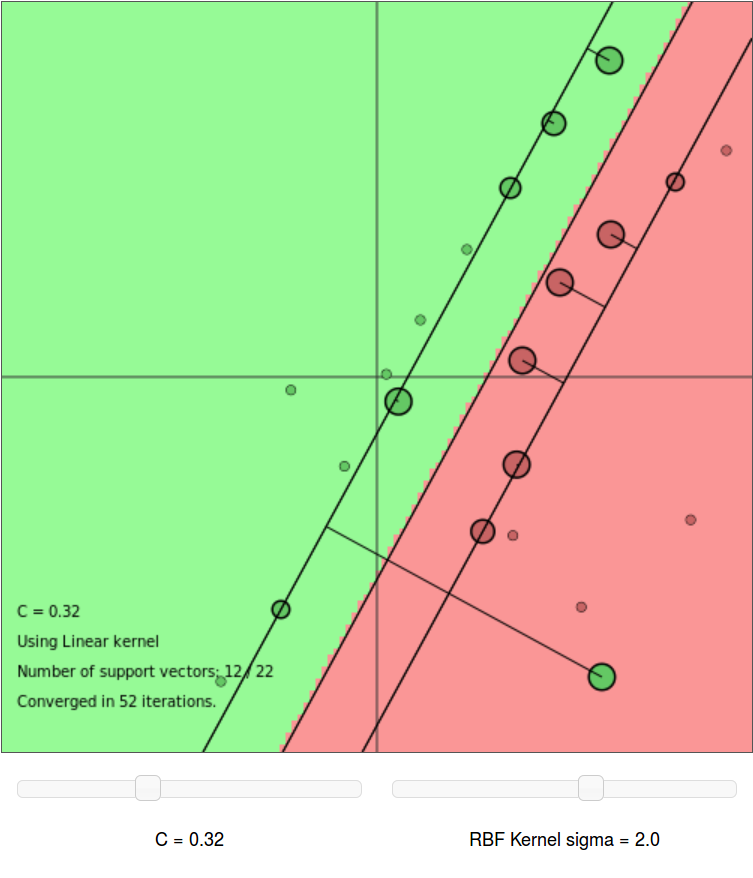
\includegraphics[width=0.33\linewidth]{../src/figure/svmjsLinSep}
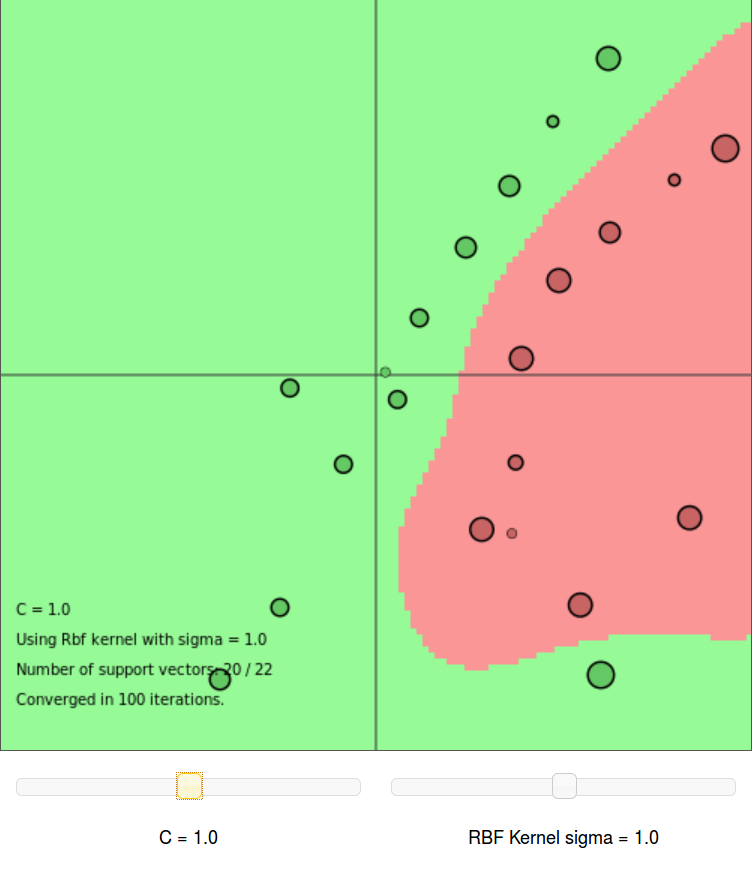
\includegraphics[width=0.33\linewidth]{../src/figure/svmjsLinRBF}
\caption{Support vector machine classification of an almost linearly separable problem using a linear and an radial basis function kernel}
\label{fig:svmjsLinRBF}
\end{figure}

If the problem is not separable, it means that classification cannot be done without error. In the underlying optimization problem slack variables have to be included in the formulation:
\begin{equation}
y_k [\mathbf{w}^T \varphi(\mathbf{x}_k) + b] \geq 1 - \xi_k
\end{equation}
Which leads to the optimization problem:
\begin{align}
\min_{w,b,\xi} J_p(w,\xi) &= \frac{1}{2}\mathbf{w}^T\mathbf{w} + c \sum_{k = 1}^N \xi_k \\
\text{such that }   y_k [\mathbf{w}^T \varphi(\mathbf{x}_k) + b] \geq 1 - \xi_k, \;\; k &= 1,\dots,N \\
\xi_k \geq 0, \;\;\; k &= 1,\dots,N 
\end{align}
Where $c$ is the positive real miss-classification penalty constant. High values of $c$ make erroneous classification more costly in terms of the merit function.  Low values make those cheaper. Using the \texttt{svmjs}\footnote{\url{http://cs.stanford.edu/people/karpathy/svmjs/demo/}} package the result of using different values of $c$ is illustrated in figure~\ref{fig:c}. Choosing the right value for $c$ is a balancing act. It is important to choose $c$ not too small. As very small values will result in underfitting the problem. The resulting classifier will ignore important features of the problem, as illustrated on the right in figure~\ref{fig:c}. On the other hand  $c$ must also not be too large. If the penalty on incorrect classification is too large the support vector machine will start to memorize noisy details, as illustrated in figure~\ref{fig:c} on the left. A good choice like the one shown in the middle captures the key points while not falling prey to the noise, while using just as many support vectors as necessary. 
\begin{figure}
\centering
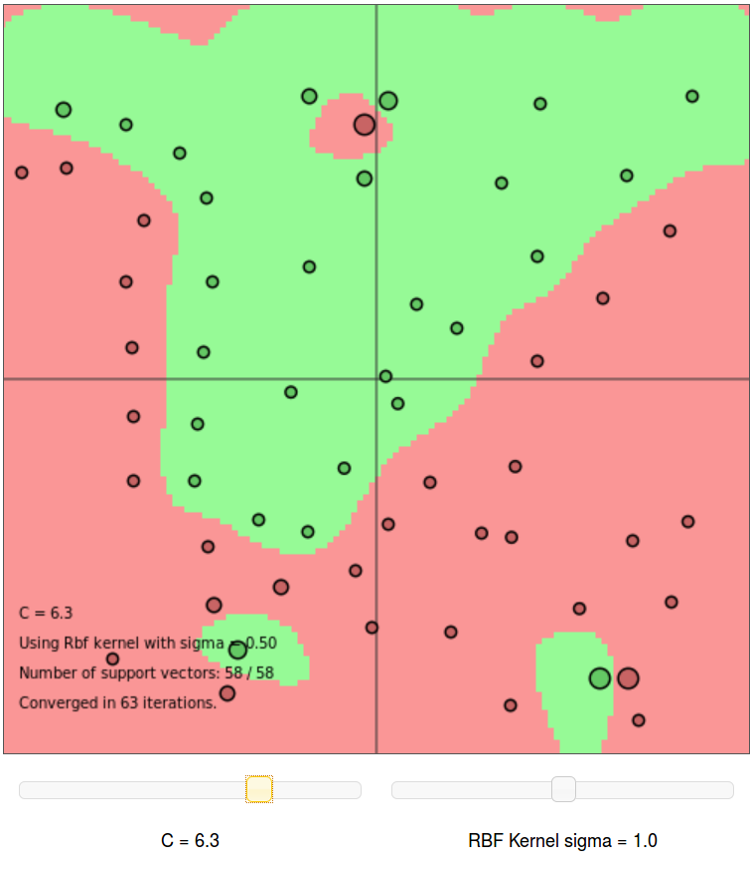
\includegraphics[width=0.3\linewidth]{../src/figure/overfit}
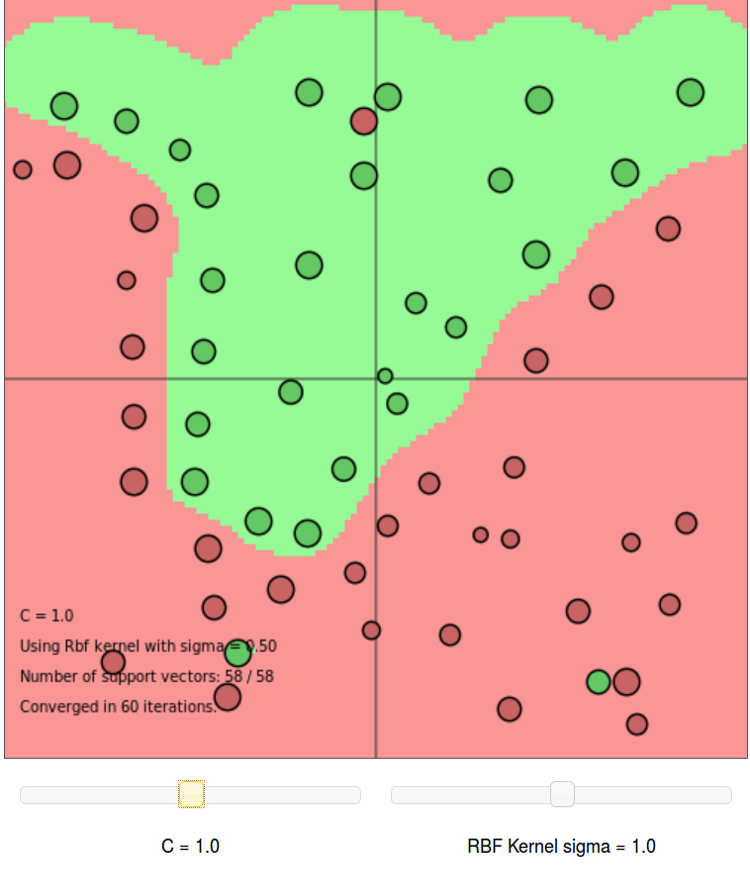
\includegraphics[width=0.3\linewidth]{../src/figure/good}
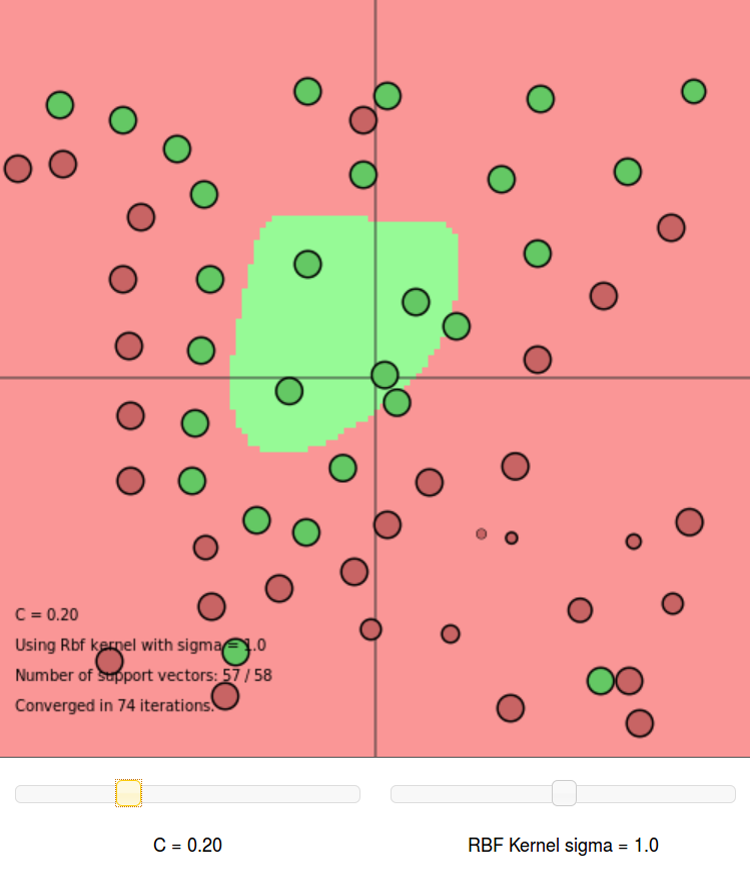
\includegraphics[width=0.3\linewidth]{../src/figure/tooLow}
\caption{The effect of a large miss-classification penalty constant $c$ (left), a good choice for $c$ (middle) and a too small penalty value (right).}
\label{fig:c}
\end{figure}
The effect of changing the kernel density $\sigma$ is explored in figure $\ref{fig:sigma}$. In this case the classification error increases significantly for very small or very large $\sigma$ values. 
\begin{figure}
\centering
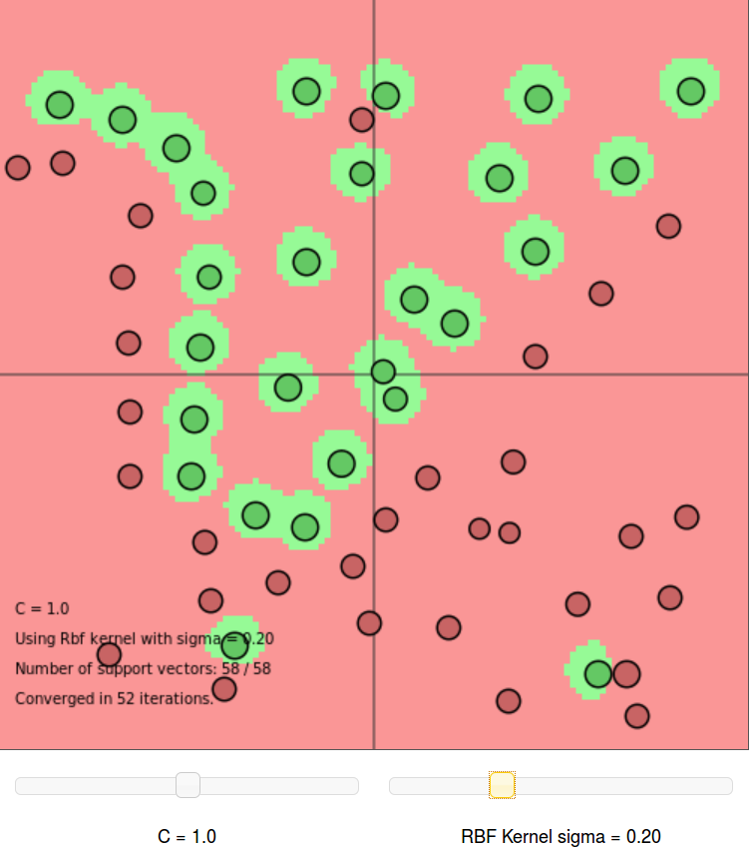
\includegraphics[width=0.3\linewidth]{../src/figure/sigmaTooSml}
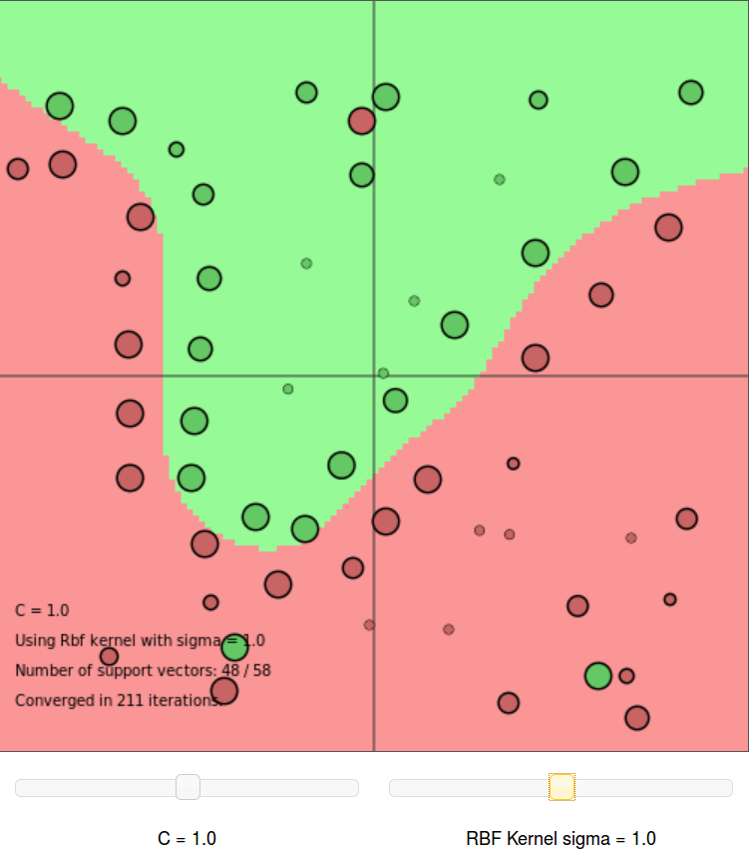
\includegraphics[width=0.3\linewidth]{../src/figure/sigmaGood}
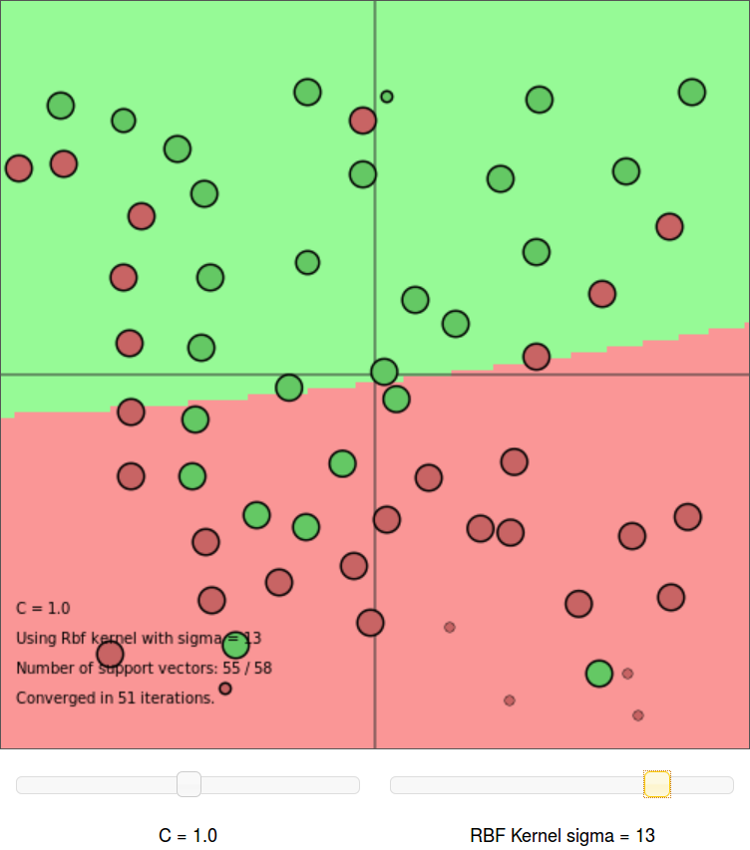
\includegraphics[width=0.3\linewidth]{../src/figure/sigmaTooLarge}
\caption{Using a  too small (left), a nicely chosen (middle) and too large (right) radial basis function parameter $\sigma$. }
\label{fig:sigma}
\end{figure}
Like choosing a good $c$ value, when picking $\sigma$ under and over-fitting considerations are important. Choosing the kernel too small as shown in figure~\ref{fig:sigma} on the left will result in over-fitting. Even tough all points are classified correctly the model misses the general overall geometry of the input data points completely. If $\sigma$ is too large under-fitting is observed in this case. Results are better in comparison to the very small $\sigma$-value but one would expect to see results of similar quality from a simple linear kernel. A good choice such as the one in figure~\ref{fig:sigma} in the middle captures the big picture while not using excessive amounts of support vectors.

\begin{figure}
\centering
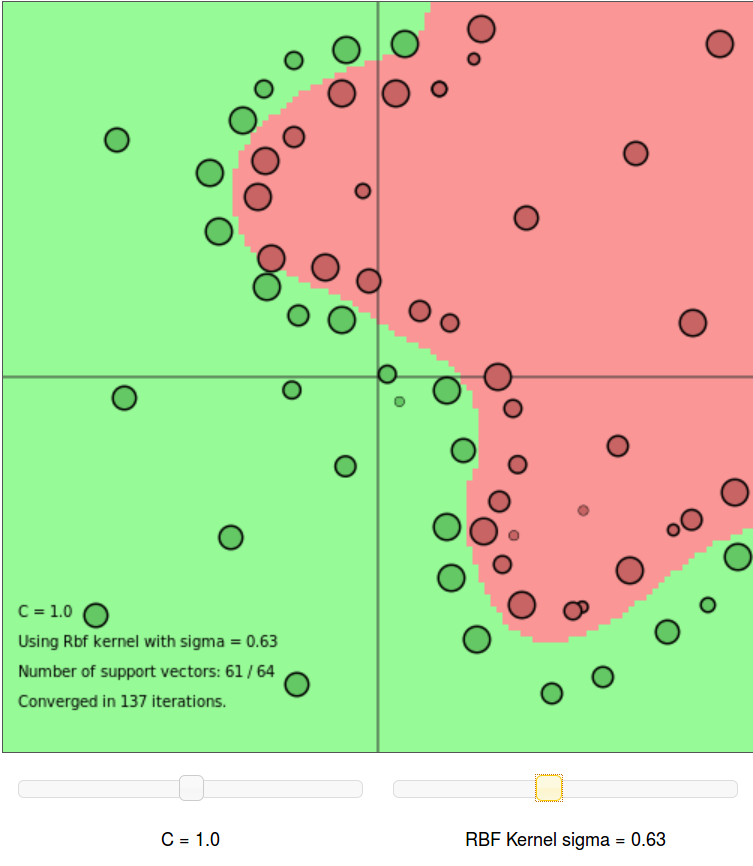
\includegraphics[width=0.33\linewidth]{../src/figure/largeRBF}
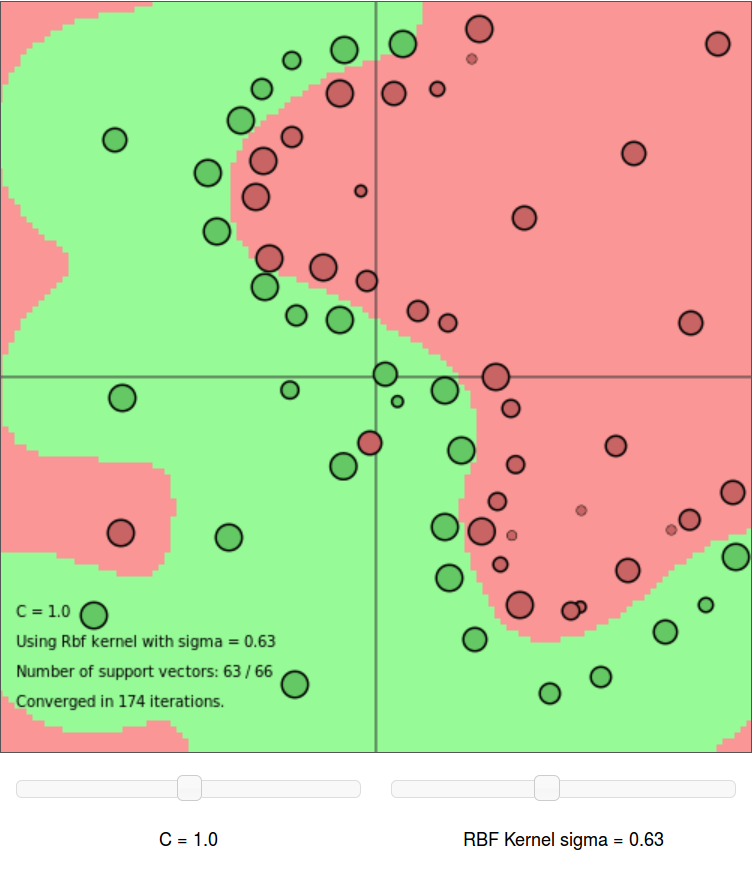
\includegraphics[width=0.33\linewidth]{../src/figure/twoNewPoints}
\caption{The effect of two additional red points on the boundary}
\label{fig:twoNewPoints}
\end{figure}
Figure~\ref{fig:twoNewPoints} illustrates the effect new data points have on the decision boundary. In the right plot two new red points have been added inside of the formerly entirely green region. The decision boundary changes if no additional miss-classification follows from this change. For the new red point close to the green boundary this cannot be done without miss-classifying the green points at the boundary, which therefore has to remain unchanged. At this point it is also important to note that \footnote{Least Squares Support Vector Machines, Suykens et al., page 32 and 41.}
\begin{align}
\mathbf{w} = \sum\limits_{k = 1}^{N} \alpha_k y_k x_x  \text{  (linear)},\\
\mathbf{w} = \sum\limits_{k = 1}^{N} \alpha_k y_k \varphi (x_k) \text{  (non-linear)}.
\end{align} 
Thus not all points contribute equally to the orientation of the decision boundary. In fact only support vectors with $\alpha_k \gg 0$ contribute, for all other points the decision bound hardly changes or remains unchanged, if $\alpha_k = 0$, if the are removed.

\section{Least Squares Support Vector machines}
In contrast to classical support vector machines, their least squares version is defined as:\footnote{Least Squares Support Vector Machines, Suykens et al., page 72.}
\begin{align}
\min_{w,b,e} J_p (w,e) &= \frac{1}{2}\mathbf{w}^T\mathbf{w} + \gamma \frac{1}{2} \sum_{k=1}^N e_k^2 \\
\text{such that } y_k [\mathbf{w}^T \varphi(\mathbf{x_k}) + b] &= 1 - e_k, \; k = 1,\dots,N
\end{align}
In comparison to the Vapnik formulation the error variable is squared and the constraint is turned into an equality constraint. After training the dual space classifier
\begin{equation}
y(x) = \text{sign}[\sum_{k = 1}^N \alpha_k y_k K(x,x_k) + b]
\end{equation}
is obtained. Least squares support vector machines (LSSVM) are an attempt to reduce the computational load for very large data sets. \\
In a first experiment the iris data set\footnote{\url{http://archive.ics.uci.edu/ml/datasets/Iris}} is used to test the LSSVM algorithm and learn more about the hyper-parameter space it works well in. The challenge here is to differentiate three types of iris plants \textit{Iris Setosa}, \textit{Iris Versicolour} and \textit{Iris Virginica}, based on the leaf dimensions: sepal length [\texttt{cm}], sepal width [\texttt{cm}], petal length [\texttt{cm}], petal width [\texttt{cm}].
\begin{figure}
\centering
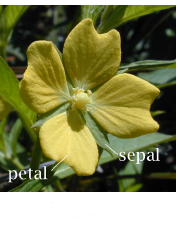
\includegraphics[width=0.25\linewidth]{../src/figure/petalSepalUP}
% This file was created by matlab2tikz.
% Minimal pgfplots version: 1.3
%
%The latest updates can be retrieved from
%  http://www.mathworks.com/matlabcentral/fileexchange/22022-matlab2tikz
%where you can also make suggestions and rate matlab2tikz.
%
\documentclass[tikz]{standalone}
\usepackage{pgfplots}
\usepackage{grffile}
\pgfplotsset{compat=newest}
\usetikzlibrary{plotmarks}
\usepackage{amsmath}

\begin{document}
\definecolor{mycolor1}{rgb}{0.00000,0.44700,0.74100}%
\definecolor{mycolor2}{rgb}{0.85000,0.32500,0.09800}%
\definecolor{mycolor3}{rgb}{0.92900,0.69400,0.12500}%
%
\begin{tikzpicture}

\begin{axis}[%
width=1.5in,
height=1.5in,
scale only axis,
xmin=1,
xmax=7,
ymin=0,
ymax=2.5,
axis x line*=bottom,
axis y line*=left,
title={petal data},
xlabel={length [\texttt{cm}]},
ylabel={width [\texttt{cm}]}
]
\addplot [color=mycolor1,only marks,mark=*,mark options={solid},forget plot]
  table[row sep=crcr]{%
1.4	0.2\\
1.4	0.2\\
1.3	0.2\\
1.5	0.2\\
1.4	0.2\\
1.7	0.4\\
1.4	0.3\\
1.5	0.2\\
1.4	0.2\\
1.5	0.1\\
1.5	0.2\\
1.6	0.2\\
1.4	0.1\\
1.1	0.1\\
1.2	0.2\\
1.5	0.4\\
1.3	0.4\\
1.4	0.3\\
1.7	0.3\\
1.5	0.3\\
1.7	0.2\\
1.5	0.4\\
1	0.2\\
1.7	0.5\\
1.9	0.2\\
1.6	0.2\\
1.6	0.4\\
1.5	0.2\\
1.4	0.2\\
1.6	0.2\\
1.6	0.2\\
1.5	0.4\\
1.5	0.1\\
1.4	0.2\\
1.5	0.1\\
1.2	0.2\\
1.3	0.2\\
1.5	0.1\\
1.3	0.2\\
1.5	0.2\\
1.3	0.3\\
1.3	0.3\\
1.3	0.2\\
1.6	0.6\\
1.9	0.4\\
1.4	0.3\\
1.6	0.2\\
1.4	0.2\\
1.5	0.2\\
1.4	0.2\\
};
\addplot [color=mycolor2,only marks,mark=*,mark options={solid},forget plot]
  table[row sep=crcr]{%
4.7	1.4\\
4.5	1.5\\
4.9	1.5\\
4	1.3\\
4.6	1.5\\
4.5	1.3\\
4.7	1.6\\
3.3	1\\
4.6	1.3\\
3.9	1.4\\
3.5	1\\
4.2	1.5\\
4	1\\
4.7	1.4\\
3.6	1.3\\
4.4	1.4\\
4.5	1.5\\
4.1	1\\
4.5	1.5\\
3.9	1.1\\
4.8	1.8\\
4	1.3\\
4.9	1.5\\
4.7	1.2\\
4.3	1.3\\
4.4	1.4\\
4.8	1.4\\
5	1.7\\
4.5	1.5\\
3.5	1\\
3.8	1.1\\
3.7	1\\
3.9	1.2\\
5.1	1.6\\
4.5	1.5\\
4.5	1.6\\
4.7	1.5\\
4.4	1.3\\
4.1	1.3\\
4	1.3\\
4.4	1.2\\
4.6	1.4\\
4	1.2\\
3.3	1\\
4.2	1.3\\
4.2	1.2\\
4.2	1.3\\
4.3	1.3\\
3	1.1\\
4.1	1.3\\
};
\addplot [color=mycolor3,only marks,mark=*,mark options={solid},forget plot]
  table[row sep=crcr]{%
6	2.5\\
5.1	1.9\\
5.9	2.1\\
5.6	1.8\\
5.8	2.2\\
6.6	2.1\\
4.5	1.7\\
6.3	1.8\\
5.8	1.8\\
6.1	2.5\\
5.1	2\\
5.3	1.9\\
5.5	2.1\\
5	2\\
5.1	2.4\\
5.3	2.3\\
5.5	1.8\\
6.7	2.2\\
6.9	2.3\\
5	1.5\\
5.7	2.3\\
4.9	2\\
6.7	2\\
4.9	1.8\\
5.7	2.1\\
6	1.8\\
4.8	1.8\\
4.9	1.8\\
5.6	2.1\\
5.8	1.6\\
6.1	1.9\\
6.4	2\\
5.6	2.2\\
5.1	1.5\\
5.6	1.4\\
6.1	2.3\\
5.6	2.4\\
5.5	1.8\\
4.8	1.8\\
5.4	2.1\\
5.6	2.4\\
5.1	2.3\\
5.1	1.9\\
5.9	2.3\\
5.7	2.5\\
5.2	2.3\\
5	1.9\\
5.2	2\\
5.4	2.3\\
5.1	1.8\\
};
\end{axis}
\end{tikzpicture}%
\end{document}
% This file was created by matlab2tikz.
% Minimal pgfplots version: 1.3
%
%The latest updates can be retrieved from
%  http://www.mathworks.com/matlabcentral/fileexchange/22022-matlab2tikz
%where you can also make suggestions and rate matlab2tikz.
%
\documentclass[tikz]{standalone}
\usepackage{pgfplots}
\usepackage{grffile}
\pgfplotsset{compat=newest}
\usetikzlibrary{plotmarks}
\usepackage{amsmath}

\begin{document}
\definecolor{mycolor1}{rgb}{0.00000,0.44700,0.74100}%
\definecolor{mycolor2}{rgb}{0.85000,0.32500,0.09800}%
\definecolor{mycolor3}{rgb}{0.92900,0.69400,0.12500}%
%
\begin{tikzpicture}

\begin{axis}[%
width=1.5in,
height=1.5in,
scale only axis,
xmin=4,
xmax=8,
ymin=2,
ymax=4.5,
axis x line*=bottom,
axis y line*=left,
title={sepal data},
xlabel={length [\texttt{cm}]},
ylabel={width [\texttt{cm}]}
]
\addplot [color=mycolor1,only marks,mark=*,mark options={solid},forget plot]
  table[row sep=crcr]{%
5.1	3.5\\
4.9	3\\
4.7	3.2\\
4.6	3.1\\
5	3.6\\
5.4	3.9\\
4.6	3.4\\
5	3.4\\
4.4	2.9\\
4.9	3.1\\
5.4	3.7\\
4.8	3.4\\
4.8	3\\
4.3	3\\
5.8	4\\
5.7	4.4\\
5.4	3.9\\
5.1	3.5\\
5.7	3.8\\
5.1	3.8\\
5.4	3.4\\
5.1	3.7\\
4.6	3.6\\
5.1	3.3\\
4.8	3.4\\
5	3\\
5	3.4\\
5.2	3.5\\
5.2	3.4\\
4.7	3.2\\
4.8	3.1\\
5.4	3.4\\
5.2	4.1\\
5.5	4.2\\
4.9	3.1\\
5	3.2\\
5.5	3.5\\
4.9	3.1\\
4.4	3\\
5.1	3.4\\
5	3.5\\
4.5	2.3\\
4.4	3.2\\
5	3.5\\
5.1	3.8\\
4.8	3\\
5.1	3.8\\
4.6	3.2\\
5.3	3.7\\
5	3.3\\
};
\addplot [color=mycolor2,only marks,mark=*,mark options={solid},forget plot]
  table[row sep=crcr]{%
7	3.2\\
6.4	3.2\\
6.9	3.1\\
5.5	2.3\\
6.5	2.8\\
5.7	2.8\\
6.3	3.3\\
4.9	2.4\\
6.6	2.9\\
5.2	2.7\\
5	2\\
5.9	3\\
6	2.2\\
6.1	2.9\\
5.6	2.9\\
6.7	3.1\\
5.6	3\\
5.8	2.7\\
6.2	2.2\\
5.6	2.5\\
5.9	3.2\\
6.1	2.8\\
6.3	2.5\\
6.1	2.8\\
6.4	2.9\\
6.6	3\\
6.8	2.8\\
6.7	3\\
6	2.9\\
5.7	2.6\\
5.5	2.4\\
5.5	2.4\\
5.8	2.7\\
6	2.7\\
5.4	3\\
6	3.4\\
6.7	3.1\\
6.3	2.3\\
5.6	3\\
5.5	2.5\\
5.5	2.6\\
6.1	3\\
5.8	2.6\\
5	2.3\\
5.6	2.7\\
5.7	3\\
5.7	2.9\\
6.2	2.9\\
5.1	2.5\\
5.7	2.8\\
};
\addplot [color=mycolor3,only marks,mark=*,mark options={solid},forget plot]
  table[row sep=crcr]{%
6.3	3.3\\
5.8	2.7\\
7.1	3\\
6.3	2.9\\
6.5	3\\
7.6	3\\
4.9	2.5\\
7.3	2.9\\
6.7	2.5\\
7.2	3.6\\
6.5	3.2\\
6.4	2.7\\
6.8	3\\
5.7	2.5\\
5.8	2.8\\
6.4	3.2\\
6.5	3\\
7.7	3.8\\
7.7	2.6\\
6	2.2\\
6.9	3.2\\
5.6	2.8\\
7.7	2.8\\
6.3	2.7\\
6.7	3.3\\
7.2	3.2\\
6.2	2.8\\
6.1	3\\
6.4	2.8\\
7.2	3\\
7.4	2.8\\
7.9	3.8\\
6.4	2.8\\
6.3	2.8\\
6.1	2.6\\
7.7	3\\
6.3	3.4\\
6.4	3.1\\
6	3\\
6.9	3.1\\
6.7	3.1\\
6.9	3.1\\
5.8	2.7\\
6.8	3.2\\
6.7	3.3\\
6.7	3\\
6.3	2.5\\
6.5	3\\
6.2	3.4\\
5.9	3\\
};
\end{axis}
\end{tikzpicture}%
\end{document}
\caption{Illustration of the difference between petal and sepal flower leafs. As well as an illustration of the data distribution with blue for \textit{Iris-setosa}, red indicating \textit{Iris-versicolor} and yellow \textit{Iris-virginica}.}
\label{fig:originalIris}
\end{figure}
Figure~\ref{fig:originalIris} shows what petal and sepal flower leafs are\footnote{\url{https://en.wikipedia.org/wiki/Sepal}} as well as the data points included in the original iris data set. For a first LSSVM trial run the simplified version shown in figure~\ref{fig:simpleIris} is used. 
\begin{figure}
\centering
% This file was created by matlab2tikz.
% Minimal pgfplots version: 1.3
%
%The latest updates can be retrieved from
%  http://www.mathworks.com/matlabcentral/fileexchange/22022-matlab2tikz
%where you can also make suggestions and rate matlab2tikz.
%
\documentclass[tikz]{standalone}
\usepackage{pgfplots}
\usepackage{grffile}
\pgfplotsset{compat=newest}
\usetikzlibrary{plotmarks}
\usepackage{amsmath}

\begin{document}
\definecolor{mycolor1}{rgb}{0.00000,0.44700,0.74100}%
\definecolor{mycolor2}{rgb}{0.85000,0.32500,0.09800}%
%
\begin{tikzpicture}

\begin{axis}[%
width=1.5in,
height=1.5in,
scale only axis,
xmin=1,
xmax=7,
ymin=0,
ymax=2.5,
title={training data},
axis x line*=bottom,
axis y line*=left,
title={petal data},
xlabel={length [\texttt{cm}]},
ylabel={width [\texttt{cm}]}
]
\addplot [color=mycolor1,only marks,mark=*,mark options={solid},forget plot]
  table[row sep=crcr]{%
1.5	0.3\\
1.5	0.2\\
6	2.5\\
6.7	2\\
4.8	1.8\\
1.5	0.2\\
1.9	0.2\\
1.3	0.3\\
1.5	0.2\\
5	1.9\\
1.4	0.3\\
5.8	2.2\\
5.1	2.4\\
4.8	1.8\\
6.6	2.1\\
5.1	1.9\\
5.6	1.4\\
1.7	0.5\\
1.5	0.2\\
1.3	0.2\\
1.6	0.2\\
1.4	0.2\\
5.6	2.4\\
1.6	0.6\\
1.3	0.2\\
5.5	1.8\\
6.1	2.5\\
1.5	0.4\\
5.1	1.8\\
5.9	2.1\\
6	1.8\\
1.5	0.1\\
5.9	2.3\\
5.6	2.1\\
5.1	2\\
1.5	0.4\\
6.1	2.3\\
1.6	0.2\\
5.2	2\\
1.5	0.1\\
6.4	2\\
1.4	0.2\\
1.4	0.2\\
5.5	1.8\\
1.4	0.2\\
1.7	0.2\\
1.5	0.2\\
4.5	1.7\\
1.4	0.1\\
6.1	1.9\\
5.5	2.1\\
1.3	0.2\\
1.5	0.4\\
1.7	0.4\\
5.8	1.8\\
1.6	0.2\\
5.1	1.5\\
1.1	0.1\\
1.4	0.2\\
1.7	0.3\\
1.6	0.4\\
5.7	2.1\\
6.7	2.2\\
6.3	1.8\\
5.3	1.9\\
1.5	0.2\\
1.4	0.2\\
};
\addplot [color=mycolor2,only marks,mark=*,mark options={solid},forget plot]
  table[row sep=crcr]{%
5	1.7\\
4.5	1.5\\
3.9	1.2\\
3.3	1\\
4.5	1.4\\
4.8	1.8\\
4	1.3\\
3.5	1\\
4.9	1.4\\
4.1	1.3\\
4.5	1.5\\
4.6	1.4\\
4.7	1.4\\
4.7	1.6\\
4.8	1.4\\
3.5	1\\
3.9	1.1\\
3.8	1.1\\
4.7	1.2\\
4.6	1.5\\
4	1\\
4	1.3\\
4.4	1.2\\
4.5	1.6\\
4.1	1\\
4.7	1.4\\
4	1.2\\
4.9	1.5\\
4.7	1.5\\
4.1	1.3\\
4.9	1.5\\
4.2	1.5\\
4.6	1.3\\
};
\end{axis}
\end{tikzpicture}%
\end{document}
\caption{Simplified iris data set, only petal leafs and only two species \textit{Iris-setosa-virginica} and \textit{Versicolor} are considered.}
\label{fig:simpleIris}
\end{figure}
\begin{figure}
\centering
% This file was created by matlab2tikz.
% Minimal pgfplots version: 1.3
%
%The latest updates can be retrieved from
%  http://www.mathworks.com/matlabcentral/fileexchange/22022-matlab2tikz
%where you can also make suggestions and rate matlab2tikz.
%
\documentclass[tikz]{standalone}
\usepackage{pgfplots}
\usepackage{grffile}
\pgfplotsset{compat=newest}
\usetikzlibrary{plotmarks}
\usepackage{amsmath}

\begin{document}
\definecolor{mycolor1}{rgb}{0.00000,0.44700,0.74100}%
\definecolor{mycolor2}{rgb}{0.85000,0.32500,0.09800}%
%
\begin{tikzpicture}

\begin{axis}[%
width=1.5in,
height=1.5in,
scale only axis,
xmin=1.078,
xmax=7.035,
xlabel={$\text{X}_{\text{1}}$},
ymin=0.0980000000000001,
ymax=2.625,
ylabel={$\text{X}_{\text{2}}$},
title={$\text{LS-SVM}_{\gamma\text{=1,}\sigma{}^\text{2}\text{=}}^{\text{lin}}$}
]
\addplot[contour prepared, contour prepared format=matlab, contour/labels=false] table[row sep=crcr] {%
%
-0.8	261\\
2.46399533333333	0.0980000000000001\\
2.46796666666667	0.0996846666666668\\
2.50370866666667	0.114846666666667\\
2.50768	0.116531333333333\\
2.543422	0.131693333333333\\
2.54739333333333	0.133378\\
2.58313533333333	0.14854\\
2.58710666666667	0.150224666666667\\
2.62284866666667	0.165386666666667\\
2.62284866666667	0.182233333333333\\
2.62682	0.183918\\
2.662562	0.19908\\
2.66653333333333	0.200764666666667\\
2.70227533333333	0.215926666666667\\
2.70624666666667	0.217611333333333\\
2.74198866666667	0.232773333333333\\
2.74596	0.234458\\
2.781702	0.24962\\
2.781702	0.266466666666667\\
2.78567333333333	0.268151333333333\\
2.82141533333333	0.283313333333333\\
2.82538666666667	0.284998\\
2.86112866666667	0.30016\\
2.8651	0.301844666666667\\
2.900842	0.317006666666667\\
2.90481333333333	0.318691333333333\\
2.94055533333333	0.333853333333333\\
2.94055533333333	0.3507\\
2.94452666666667	0.352384666666667\\
2.98026866666667	0.367546666666667\\
2.98424	0.369231333333333\\
3.019982	0.384393333333333\\
3.02395333333333	0.386078\\
3.05969533333333	0.40124\\
3.06366666666667	0.402924666666667\\
3.09940866666667	0.418086666666667\\
3.09940866666667	0.434933333333333\\
3.10338	0.436618\\
3.139122	0.45178\\
3.14309333333333	0.453464666666667\\
3.17883533333333	0.468626666666667\\
3.18280666666667	0.470311333333333\\
3.21854866666667	0.485473333333333\\
3.22252	0.487158\\
3.258262	0.50232\\
3.258262	0.519166666666667\\
3.26223333333333	0.520851333333333\\
3.29797533333333	0.536013333333333\\
3.30194666666667	0.537698\\
3.33768866666667	0.55286\\
3.34166	0.554544666666667\\
3.377402	0.569706666666667\\
3.38137333333333	0.571391333333333\\
3.41711533333333	0.586553333333333\\
3.41711533333333	0.6034\\
3.42108666666667	0.605084666666667\\
3.45682866666667	0.620246666666667\\
3.4608	0.621931333333333\\
3.496542	0.637093333333333\\
3.50051333333333	0.638778\\
3.53625533333333	0.65394\\
3.53625533333333	0.670786666666667\\
3.54022666666667	0.672471333333333\\
3.57596866666667	0.687633333333333\\
3.57994	0.689318\\
3.615682	0.70448\\
3.61965333333333	0.706164666666667\\
3.65539533333333	0.721326666666667\\
3.65936666666667	0.723011333333333\\
3.69510866666667	0.738173333333333\\
3.69510866666667	0.75502\\
3.69908	0.756704666666667\\
3.734822	0.771866666666667\\
3.73879333333333	0.773551333333333\\
3.77453533333333	0.788713333333333\\
3.77850666666667	0.790398\\
3.81424866666667	0.80556\\
3.81822	0.807244666666667\\
3.853962	0.822406666666667\\
3.853962	0.839253333333333\\
3.85793333333333	0.840938\\
3.89367533333333	0.8561\\
3.89764666666667	0.857784666666667\\
3.93338866666667	0.872946666666667\\
3.93736	0.874631333333333\\
3.973102	0.889793333333333\\
3.97707333333333	0.891478\\
4.01281533333333	0.90664\\
4.01281533333333	0.923486666666667\\
4.01678666666667	0.925171333333333\\
4.05252866666667	0.940333333333333\\
4.0565	0.942018\\
4.092242	0.95718\\
4.09621333333333	0.958864666666667\\
4.13195533333333	0.974026666666667\\
4.13592666666667	0.975711333333333\\
4.17166866666667	0.990873333333333\\
4.17166866666667	1.00772\\
4.17564	1.00940466666667\\
4.211382	1.02456666666667\\
4.21535333333333	1.02625133333333\\
4.25109533333333	1.04141333333333\\
4.25506666666667	1.043098\\
4.29080866666667	1.05826\\
4.29478	1.05994466666667\\
4.330522	1.07510666666667\\
4.330522	1.09195333333333\\
4.33449333333333	1.093638\\
4.37023533333333	1.1088\\
4.37420666666667	1.11048466666667\\
4.40994866666667	1.12564666666667\\
4.41392	1.12733133333333\\
4.449662	1.14249333333333\\
4.45363333333333	1.144178\\
4.48937533333333	1.15934\\
4.48937533333333	1.17618666666667\\
4.49334666666667	1.17787133333333\\
4.52908866666667	1.19303333333333\\
4.53306	1.194718\\
4.568802	1.20988\\
4.57277333333333	1.21156466666667\\
4.60851533333333	1.22672666666667\\
4.61248666666667	1.22841133333333\\
4.64822866666667	1.24357333333333\\
4.64822866666667	1.26042\\
4.6522	1.26210466666667\\
4.687942	1.27726666666667\\
4.69191333333333	1.27895133333333\\
4.72765533333333	1.29411333333333\\
4.73162666666667	1.295798\\
4.76736866666667	1.31096\\
4.77134	1.31264466666667\\
4.807082	1.32780666666667\\
4.807082	1.34465333333333\\
4.81105333333333	1.346338\\
4.84679533333333	1.3615\\
4.85076666666667	1.36318466666667\\
4.88650866666667	1.37834666666667\\
4.89048	1.38003133333333\\
4.926222	1.39519333333333\\
4.93019333333333	1.396878\\
4.96593533333333	1.41204\\
4.96593533333333	1.42888666666667\\
4.96990666666667	1.43057133333333\\
5.00564866666667	1.44573333333333\\
5.00962	1.447418\\
5.045362	1.46258\\
5.04933333333333	1.46426466666667\\
5.08507533333333	1.47942666666667\\
5.08507533333333	1.49627333333333\\
5.08904666666667	1.497958\\
5.12478866666667	1.51312\\
5.12876	1.51480466666667\\
5.164502	1.52996666666667\\
5.16847333333333	1.53165133333333\\
5.20421533333333	1.54681333333333\\
5.20818666666667	1.548498\\
5.24392866666667	1.56366\\
5.24392866666667	1.58050666666667\\
5.2479	1.58219133333333\\
5.283642	1.59735333333333\\
5.28761333333333	1.599038\\
5.32335533333333	1.6142\\
5.32732666666667	1.61588466666667\\
5.36306866666667	1.63104666666667\\
5.36704	1.63273133333333\\
5.402782	1.64789333333333\\
5.402782	1.66474\\
5.40675333333333	1.66642466666667\\
5.44249533333333	1.68158666666667\\
5.44646666666667	1.68327133333333\\
5.48220866666667	1.69843333333333\\
5.48618	1.700118\\
5.521922	1.71528\\
5.52589333333333	1.71696466666667\\
5.56163533333333	1.73212666666667\\
5.56163533333333	1.74897333333333\\
5.56560666666667	1.750658\\
5.60134866666667	1.76582\\
5.60532	1.76750466666667\\
5.641062	1.78266666666667\\
5.64503333333333	1.78435133333333\\
5.68077533333333	1.79951333333333\\
5.68474666666667	1.801198\\
5.72048866666667	1.81636\\
5.72048866666667	1.83320666666667\\
5.72446	1.83489133333333\\
5.760202	1.85005333333333\\
5.76417333333333	1.851738\\
5.79991533333333	1.8669\\
5.80388666666667	1.86858466666667\\
5.83962866666667	1.88374666666667\\
5.8436	1.88543133333333\\
5.879342	1.90059333333333\\
5.879342	1.91744\\
5.88331333333333	1.91912466666667\\
5.91905533333333	1.93428666666667\\
5.92302666666667	1.93597133333333\\
5.95876866666667	1.95113333333333\\
5.96274	1.952818\\
5.998482	1.96798\\
6.00245333333333	1.96966466666667\\
6.03819533333333	1.98482666666667\\
6.03819533333333	2.00167333333333\\
6.04216666666667	2.003358\\
6.07790866666667	2.01852\\
6.08188	2.02020466666667\\
6.117622	2.03536666666667\\
6.12159333333333	2.03705133333333\\
6.15733533333333	2.05221333333333\\
6.16130666666667	2.053898\\
6.19704866666667	2.06906\\
6.19704866666667	2.08590666666667\\
6.20102	2.08759133333333\\
6.236762	2.10275333333333\\
6.24073333333333	2.104438\\
6.27647533333333	2.1196\\
6.28044666666667	2.12128466666667\\
6.31618866666667	2.13644666666667\\
6.32016	2.13813133333333\\
6.355902	2.15329333333333\\
6.355902	2.17014\\
6.35987333333333	2.17182466666667\\
6.39561533333333	2.18698666666667\\
6.39958666666667	2.18867133333333\\
6.43532866666667	2.20383333333333\\
6.4393	2.205518\\
6.475042	2.22068\\
6.475042	2.23752666666667\\
6.47901333333333	2.23921133333333\\
6.51475533333333	2.25437333333333\\
6.51872666666667	2.256058\\
6.55446866666667	2.27122\\
6.55844	2.27290466666667\\
6.594182	2.28806666666667\\
6.59815333333333	2.28975133333333\\
6.63389533333333	2.30491333333333\\
6.63389533333333	2.32176\\
6.63786666666667	2.32344466666667\\
6.67360866666667	2.33860666666667\\
6.67758	2.34029133333333\\
6.713322	2.35545333333333\\
6.71729333333333	2.357138\\
6.75303533333333	2.3723\\
6.75700666666667	2.37398466666667\\
6.79274866666667	2.38914666666667\\
6.79274866666667	2.40599333333333\\
6.79672	2.407678\\
6.832462	2.42284\\
6.83643333333333	2.42452466666667\\
6.87217533333333	2.43968666666667\\
6.87614666666667	2.44137133333333\\
6.91188866666667	2.45653333333333\\
6.91586	2.458218\\
6.951602	2.47338\\
6.951602	2.49022666666667\\
6.95557333333333	2.49191133333333\\
6.99131533333333	2.50707333333333\\
6.99528666666667	2.508758\\
7.03102866666667	2.52392\\
7.035	2.52560466666667\\
-0.6	261\\
2.460024	0.0980000000000001\\
2.46796666666667	0.101369333333333\\
2.49973733333333	0.114846666666667\\
2.50768	0.118216\\
2.53945066666667	0.131693333333333\\
2.54739333333333	0.135062666666667\\
2.579164	0.14854\\
2.58710666666667	0.151909333333333\\
2.61887733333333	0.165386666666667\\
2.61887733333333	0.182233333333333\\
2.62682	0.185602666666667\\
2.65859066666667	0.19908\\
2.66653333333333	0.202449333333333\\
2.698304	0.215926666666667\\
2.70624666666667	0.219296\\
2.73801733333333	0.232773333333333\\
2.74596	0.236142666666667\\
2.77773066666667	0.24962\\
2.77773066666667	0.266466666666667\\
2.78567333333333	0.269836\\
2.817444	0.283313333333333\\
2.82538666666667	0.286682666666667\\
2.85715733333333	0.30016\\
2.8651	0.303529333333333\\
2.89687066666667	0.317006666666667\\
2.90481333333333	0.320376\\
2.936584	0.333853333333333\\
2.936584	0.3507\\
2.94452666666667	0.354069333333333\\
2.97629733333333	0.367546666666667\\
2.98424	0.370916\\
3.01601066666667	0.384393333333333\\
3.02395333333333	0.387762666666667\\
3.055724	0.40124\\
3.06366666666667	0.404609333333333\\
3.09543733333333	0.418086666666667\\
3.09543733333333	0.434933333333333\\
3.10338	0.438302666666667\\
3.13515066666667	0.45178\\
3.14309333333333	0.455149333333333\\
3.174864	0.468626666666667\\
3.18280666666667	0.471996\\
3.21457733333333	0.485473333333333\\
3.22252	0.488842666666667\\
3.25429066666667	0.50232\\
3.25429066666667	0.519166666666667\\
3.26223333333333	0.522536\\
3.294004	0.536013333333333\\
3.30194666666667	0.539382666666667\\
3.33371733333333	0.55286\\
3.34166	0.556229333333333\\
3.37343066666667	0.569706666666667\\
3.38137333333333	0.573076\\
3.413144	0.586553333333333\\
3.413144	0.6034\\
3.42108666666667	0.606769333333333\\
3.45285733333333	0.620246666666667\\
3.4608	0.623616\\
3.49257066666667	0.637093333333333\\
3.50051333333333	0.640462666666667\\
3.532284	0.65394\\
3.532284	0.670786666666667\\
3.54022666666667	0.674156\\
3.57199733333333	0.687633333333333\\
3.57994	0.691002666666667\\
3.61171066666667	0.70448\\
3.61965333333333	0.707849333333333\\
3.651424	0.721326666666667\\
3.65936666666667	0.724696\\
3.69113733333333	0.738173333333333\\
3.69113733333333	0.75502\\
3.69908	0.758389333333333\\
3.73085066666667	0.771866666666667\\
3.73879333333333	0.775236\\
3.770564	0.788713333333333\\
3.77850666666667	0.792082666666667\\
3.81027733333333	0.80556\\
3.81822	0.808929333333333\\
3.84999066666667	0.822406666666667\\
3.84999066666667	0.839253333333333\\
3.85793333333333	0.842622666666667\\
3.889704	0.8561\\
3.89764666666667	0.859469333333333\\
3.92941733333333	0.872946666666667\\
3.93736	0.876316\\
3.96913066666667	0.889793333333333\\
3.97707333333333	0.893162666666667\\
4.008844	0.90664\\
4.008844	0.923486666666667\\
4.01678666666667	0.926856\\
4.04855733333333	0.940333333333333\\
4.0565	0.943702666666667\\
4.08827066666667	0.95718\\
4.09621333333333	0.960549333333333\\
4.127984	0.974026666666667\\
4.13592666666667	0.977396\\
4.16769733333333	0.990873333333333\\
4.16769733333333	1.00772\\
4.17564	1.01108933333333\\
4.20741066666667	1.02456666666667\\
4.21535333333333	1.027936\\
4.247124	1.04141333333333\\
4.25506666666667	1.04478266666667\\
4.28683733333333	1.05826\\
4.29478	1.06162933333333\\
4.32655066666667	1.07510666666667\\
4.32655066666667	1.09195333333333\\
4.33449333333333	1.09532266666667\\
4.366264	1.1088\\
4.37420666666667	1.11216933333333\\
4.40597733333333	1.12564666666667\\
4.41392	1.129016\\
4.44569066666667	1.14249333333333\\
4.45363333333333	1.14586266666667\\
4.485404	1.15934\\
4.485404	1.17618666666667\\
4.49334666666667	1.179556\\
4.52511733333333	1.19303333333333\\
4.53306	1.19640266666667\\
4.56483066666667	1.20988\\
4.57277333333333	1.21324933333333\\
4.604544	1.22672666666667\\
4.61248666666667	1.230096\\
4.64425733333333	1.24357333333333\\
4.64425733333333	1.26042\\
4.6522	1.26378933333333\\
4.68397066666667	1.27726666666667\\
4.69191333333333	1.280636\\
4.723684	1.29411333333333\\
4.73162666666667	1.29748266666667\\
4.76339733333333	1.31096\\
4.77134	1.31432933333333\\
4.80311066666667	1.32780666666667\\
4.80311066666667	1.34465333333333\\
4.81105333333333	1.34802266666667\\
4.842824	1.3615\\
4.85076666666667	1.36486933333333\\
4.88253733333333	1.37834666666667\\
4.89048	1.381716\\
4.92225066666667	1.39519333333333\\
4.93019333333333	1.39856266666667\\
4.961964	1.41204\\
4.961964	1.42888666666667\\
4.96990666666667	1.432256\\
5.00167733333333	1.44573333333333\\
5.00962	1.44910266666667\\
5.04139066666667	1.46258\\
5.04933333333333	1.46594933333333\\
5.081104	1.47942666666667\\
5.081104	1.49627333333333\\
5.08904666666667	1.49964266666667\\
5.12081733333333	1.51312\\
5.12876	1.51648933333333\\
5.16053066666667	1.52996666666667\\
5.16847333333333	1.533336\\
5.200244	1.54681333333333\\
5.20818666666667	1.55018266666667\\
5.23995733333333	1.56366\\
5.23995733333333	1.58050666666667\\
5.2479	1.583876\\
5.27967066666667	1.59735333333333\\
5.28761333333333	1.60072266666667\\
5.319384	1.6142\\
5.32732666666667	1.61756933333333\\
5.35909733333333	1.63104666666667\\
5.36704	1.634416\\
5.39881066666667	1.64789333333333\\
5.39881066666667	1.66474\\
5.40675333333333	1.66810933333333\\
5.438524	1.68158666666667\\
5.44646666666667	1.684956\\
5.47823733333333	1.69843333333333\\
5.48618	1.70180266666667\\
5.51795066666667	1.71528\\
5.52589333333333	1.71864933333333\\
5.557664	1.73212666666667\\
5.557664	1.74897333333333\\
5.56560666666667	1.75234266666667\\
5.59737733333333	1.76582\\
5.60532	1.76918933333333\\
5.63709066666667	1.78266666666667\\
5.64503333333333	1.786036\\
5.676804	1.79951333333333\\
5.68474666666667	1.80288266666667\\
5.71651733333333	1.81636\\
5.71651733333333	1.83320666666667\\
5.72446	1.836576\\
5.75623066666667	1.85005333333333\\
5.76417333333333	1.85342266666667\\
5.795944	1.8669\\
5.80388666666667	1.87026933333333\\
5.83565733333333	1.88374666666667\\
5.8436	1.887116\\
5.87537066666667	1.90059333333333\\
5.87537066666667	1.91744\\
5.88331333333333	1.92080933333333\\
5.915084	1.93428666666667\\
5.92302666666667	1.937656\\
5.95479733333333	1.95113333333333\\
5.96274	1.95450266666667\\
5.99451066666667	1.96798\\
6.00245333333333	1.97134933333333\\
6.034224	1.98482666666667\\
6.034224	2.00167333333333\\
6.04216666666667	2.00504266666667\\
6.07393733333333	2.01852\\
6.08188	2.02188933333333\\
6.11365066666667	2.03536666666667\\
6.12159333333333	2.038736\\
6.153364	2.05221333333333\\
6.16130666666667	2.05558266666667\\
6.19307733333333	2.06906\\
6.19307733333333	2.08590666666667\\
6.20102	2.089276\\
6.23279066666667	2.10275333333333\\
6.24073333333333	2.10612266666667\\
6.272504	2.1196\\
6.28044666666667	2.12296933333333\\
6.31221733333333	2.13644666666667\\
6.32016	2.139816\\
6.35193066666667	2.15329333333333\\
6.35193066666667	2.17014\\
6.35987333333333	2.17350933333333\\
6.391644	2.18698666666667\\
6.39958666666667	2.190356\\
6.43135733333333	2.20383333333333\\
6.4393	2.20720266666667\\
6.47107066666667	2.22068\\
6.47107066666667	2.23752666666667\\
6.47901333333333	2.240896\\
6.510784	2.25437333333333\\
6.51872666666667	2.25774266666667\\
6.55049733333333	2.27122\\
6.55844	2.27458933333333\\
6.59021066666667	2.28806666666667\\
6.59815333333333	2.291436\\
6.629924	2.30491333333333\\
6.629924	2.32176\\
6.63786666666667	2.32512933333333\\
6.66963733333333	2.33860666666667\\
6.67758	2.341976\\
6.70935066666667	2.35545333333333\\
6.71729333333333	2.35882266666667\\
6.749064	2.3723\\
6.75700666666667	2.37566933333333\\
6.78877733333333	2.38914666666667\\
6.78877733333333	2.40599333333333\\
6.79672	2.40936266666667\\
6.82849066666667	2.42284\\
6.83643333333333	2.42620933333333\\
6.868204	2.43968666666667\\
6.87614666666667	2.443056\\
6.90791733333333	2.45653333333333\\
6.91586	2.45990266666667\\
6.94763066666667	2.47338\\
6.94763066666667	2.49022666666667\\
6.95557333333333	2.493596\\
6.987344	2.50707333333333\\
6.99528666666667	2.51044266666667\\
7.02705733333333	2.52392\\
7.035	2.52728933333333\\
-0.4	261\\
2.45605266666667	0.0980000000000001\\
2.46796666666667	0.103054\\
2.495766	0.114846666666667\\
2.50768	0.119900666666667\\
2.53547933333333	0.131693333333333\\
2.54739333333333	0.136747333333333\\
2.57519266666667	0.14854\\
2.58710666666667	0.153594\\
2.614906	0.165386666666667\\
2.614906	0.182233333333333\\
2.62682	0.187287333333333\\
2.65461933333333	0.19908\\
2.66653333333333	0.204134\\
2.69433266666667	0.215926666666667\\
2.70624666666667	0.220980666666667\\
2.734046	0.232773333333333\\
2.74596	0.237827333333333\\
2.77375933333333	0.24962\\
2.77375933333333	0.266466666666667\\
2.78567333333333	0.271520666666667\\
2.81347266666667	0.283313333333333\\
2.82538666666667	0.288367333333333\\
2.853186	0.30016\\
2.8651	0.305214\\
2.89289933333333	0.317006666666667\\
2.90481333333333	0.322060666666667\\
2.93261266666667	0.333853333333333\\
2.93261266666667	0.3507\\
2.94452666666667	0.355754\\
2.972326	0.367546666666667\\
2.98424	0.372600666666667\\
3.01203933333333	0.384393333333333\\
3.02395333333333	0.389447333333333\\
3.05175266666667	0.40124\\
3.06366666666667	0.406294\\
3.091466	0.418086666666667\\
3.091466	0.434933333333333\\
3.10338	0.439987333333333\\
3.13117933333333	0.45178\\
3.14309333333333	0.456834\\
3.17089266666667	0.468626666666667\\
3.18280666666667	0.473680666666667\\
3.210606	0.485473333333333\\
3.22252	0.490527333333333\\
3.25031933333333	0.50232\\
3.25031933333333	0.519166666666667\\
3.26223333333333	0.524220666666667\\
3.29003266666667	0.536013333333333\\
3.30194666666667	0.541067333333333\\
3.329746	0.55286\\
3.34166	0.557914\\
3.36945933333333	0.569706666666667\\
3.38137333333333	0.574760666666667\\
3.40917266666667	0.586553333333333\\
3.40917266666667	0.6034\\
3.42108666666667	0.608454\\
3.448886	0.620246666666667\\
3.4608	0.625300666666667\\
3.48859933333333	0.637093333333333\\
3.50051333333333	0.642147333333333\\
3.52831266666667	0.65394\\
3.52831266666667	0.670786666666667\\
3.54022666666667	0.675840666666667\\
3.568026	0.687633333333333\\
3.57994	0.692687333333333\\
3.60773933333333	0.70448\\
3.61965333333333	0.709534\\
3.64745266666667	0.721326666666667\\
3.65936666666667	0.726380666666667\\
3.687166	0.738173333333333\\
3.687166	0.75502\\
3.69908	0.760074\\
3.72687933333333	0.771866666666667\\
3.73879333333333	0.776920666666667\\
3.76659266666667	0.788713333333333\\
3.77850666666667	0.793767333333333\\
3.806306	0.80556\\
3.81822	0.810614\\
3.84601933333333	0.822406666666667\\
3.84601933333333	0.839253333333333\\
3.85793333333333	0.844307333333333\\
3.88573266666667	0.8561\\
3.89764666666667	0.861154\\
3.925446	0.872946666666667\\
3.93736	0.878000666666667\\
3.96515933333333	0.889793333333333\\
3.97707333333333	0.894847333333333\\
4.00487266666667	0.90664\\
4.00487266666667	0.923486666666667\\
4.01678666666667	0.928540666666667\\
4.044586	0.940333333333333\\
4.0565	0.945387333333333\\
4.08429933333333	0.95718\\
4.09621333333333	0.962234\\
4.12401266666667	0.974026666666667\\
4.13592666666667	0.979080666666667\\
4.163726	0.990873333333333\\
4.163726	1.00772\\
4.17564	1.012774\\
4.20343933333333	1.02456666666667\\
4.21535333333333	1.02962066666667\\
4.24315266666667	1.04141333333333\\
4.25506666666667	1.04646733333333\\
4.282866	1.05826\\
4.29478	1.063314\\
4.32257933333333	1.07510666666667\\
4.32257933333333	1.09195333333333\\
4.33449333333333	1.09700733333333\\
4.36229266666667	1.1088\\
4.37420666666667	1.113854\\
4.402006	1.12564666666667\\
4.41392	1.13070066666667\\
4.44171933333333	1.14249333333333\\
4.45363333333333	1.14754733333333\\
4.48143266666667	1.15934\\
4.48143266666667	1.17618666666667\\
4.49334666666667	1.18124066666667\\
4.521146	1.19303333333333\\
4.53306	1.19808733333333\\
4.56085933333333	1.20988\\
4.57277333333333	1.214934\\
4.60057266666667	1.22672666666667\\
4.61248666666667	1.23178066666667\\
4.640286	1.24357333333333\\
4.640286	1.26042\\
4.6522	1.265474\\
4.67999933333333	1.27726666666667\\
4.69191333333333	1.28232066666667\\
4.71971266666667	1.29411333333333\\
4.73162666666667	1.29916733333333\\
4.759426	1.31096\\
4.77134	1.316014\\
4.79913933333333	1.32780666666667\\
4.79913933333333	1.34465333333333\\
4.81105333333333	1.34970733333333\\
4.83885266666667	1.3615\\
4.85076666666667	1.366554\\
4.878566	1.37834666666667\\
4.89048	1.38340066666667\\
4.91827933333333	1.39519333333333\\
4.93019333333333	1.40024733333333\\
4.95799266666667	1.41204\\
4.95799266666667	1.42888666666667\\
4.96990666666667	1.43394066666667\\
4.997706	1.44573333333333\\
5.00962	1.45078733333333\\
5.03741933333333	1.46258\\
5.04933333333333	1.467634\\
5.07713266666667	1.47942666666667\\
5.07713266666667	1.49627333333333\\
5.08904666666667	1.50132733333333\\
5.116846	1.51312\\
5.12876	1.518174\\
5.15655933333333	1.52996666666667\\
5.16847333333333	1.53502066666667\\
5.19627266666667	1.54681333333333\\
5.20818666666667	1.55186733333333\\
5.235986	1.56366\\
5.235986	1.58050666666667\\
5.2479	1.58556066666667\\
5.27569933333333	1.59735333333333\\
5.28761333333333	1.60240733333333\\
5.31541266666667	1.6142\\
5.32732666666667	1.619254\\
5.355126	1.63104666666667\\
5.36704	1.63610066666667\\
5.39483933333333	1.64789333333333\\
5.39483933333333	1.66474\\
5.40675333333333	1.669794\\
5.43455266666667	1.68158666666667\\
5.44646666666667	1.68664066666667\\
5.474266	1.69843333333333\\
5.48618	1.70348733333333\\
5.51397933333333	1.71528\\
5.52589333333333	1.720334\\
5.55369266666667	1.73212666666667\\
5.55369266666667	1.74897333333333\\
5.56560666666667	1.75402733333333\\
5.593406	1.76582\\
5.60532	1.770874\\
5.63311933333333	1.78266666666667\\
5.64503333333333	1.78772066666667\\
5.67283266666667	1.79951333333333\\
5.68474666666667	1.80456733333333\\
5.712546	1.81636\\
5.712546	1.83320666666667\\
5.72446	1.83826066666667\\
5.75225933333333	1.85005333333333\\
5.76417333333333	1.85510733333333\\
5.79197266666667	1.8669\\
5.80388666666667	1.871954\\
5.831686	1.88374666666667\\
5.8436	1.88880066666667\\
5.87139933333333	1.90059333333333\\
5.87139933333333	1.91744\\
5.88331333333333	1.922494\\
5.91111266666667	1.93428666666667\\
5.92302666666667	1.93934066666667\\
5.950826	1.95113333333333\\
5.96274	1.95618733333333\\
5.99053933333333	1.96798\\
6.00245333333333	1.973034\\
6.03025266666667	1.98482666666667\\
6.03025266666667	2.00167333333333\\
6.04216666666667	2.00672733333333\\
6.069966	2.01852\\
6.08188	2.023574\\
6.10967933333333	2.03536666666667\\
6.12159333333333	2.04042066666667\\
6.14939266666667	2.05221333333333\\
6.16130666666667	2.05726733333333\\
6.189106	2.06906\\
6.189106	2.08590666666667\\
6.20102	2.09096066666667\\
6.22881933333333	2.10275333333333\\
6.24073333333333	2.10780733333333\\
6.26853266666667	2.1196\\
6.28044666666667	2.124654\\
6.308246	2.13644666666667\\
6.32016	2.14150066666667\\
6.34795933333333	2.15329333333333\\
6.34795933333333	2.17014\\
6.35987333333333	2.175194\\
6.38767266666667	2.18698666666667\\
6.39958666666667	2.19204066666667\\
6.427386	2.20383333333333\\
6.4393	2.20888733333333\\
6.46709933333333	2.22068\\
6.46709933333333	2.23752666666667\\
6.47901333333333	2.24258066666667\\
6.50681266666667	2.25437333333333\\
6.51872666666667	2.25942733333333\\
6.546526	2.27122\\
6.55844	2.276274\\
6.58623933333333	2.28806666666667\\
6.59815333333333	2.29312066666667\\
6.62595266666667	2.30491333333333\\
6.62595266666667	2.32176\\
6.63786666666667	2.326814\\
6.665666	2.33860666666667\\
6.67758	2.34366066666667\\
6.70537933333333	2.35545333333333\\
6.71729333333333	2.36050733333333\\
6.74509266666667	2.3723\\
6.75700666666667	2.377354\\
6.784806	2.38914666666667\\
6.784806	2.40599333333333\\
6.79672	2.41104733333333\\
6.82451933333333	2.42284\\
6.83643333333333	2.427894\\
6.86423266666667	2.43968666666667\\
6.87614666666667	2.44474066666667\\
6.903946	2.45653333333333\\
6.91586	2.46158733333333\\
6.94365933333333	2.47338\\
6.94365933333333	2.49022666666667\\
6.95557333333333	2.49528066666667\\
6.98337266666667	2.50707333333333\\
6.99528666666667	2.51212733333333\\
7.023086	2.52392\\
7.035	2.528974\\
-0.2	261\\
2.45208133333333	0.0980000000000001\\
2.46796666666667	0.104738666666667\\
2.49179466666667	0.114846666666667\\
2.50768	0.121585333333333\\
2.531508	0.131693333333333\\
2.54739333333333	0.138432\\
2.57122133333333	0.14854\\
2.58710666666667	0.155278666666667\\
2.61093466666667	0.165386666666667\\
2.61093466666667	0.182233333333333\\
2.62682	0.188972\\
2.650648	0.19908\\
2.66653333333333	0.205818666666667\\
2.69036133333333	0.215926666666667\\
2.70624666666667	0.222665333333333\\
2.73007466666667	0.232773333333333\\
2.74596	0.239512\\
2.769788	0.24962\\
2.769788	0.266466666666667\\
2.78567333333333	0.273205333333333\\
2.80950133333333	0.283313333333333\\
2.82538666666667	0.290052\\
2.84921466666667	0.30016\\
2.8651	0.306898666666667\\
2.888928	0.317006666666667\\
2.90481333333333	0.323745333333333\\
2.92864133333333	0.333853333333333\\
2.92864133333333	0.3507\\
2.94452666666667	0.357438666666667\\
2.96835466666667	0.367546666666667\\
2.98424	0.374285333333333\\
3.008068	0.384393333333333\\
3.02395333333333	0.391132\\
3.04778133333333	0.40124\\
3.06366666666667	0.407978666666667\\
3.08749466666667	0.418086666666667\\
3.08749466666667	0.434933333333333\\
3.10338	0.441672\\
3.127208	0.45178\\
3.14309333333333	0.458518666666667\\
3.16692133333333	0.468626666666667\\
3.18280666666667	0.475365333333333\\
3.20663466666667	0.485473333333333\\
3.22252	0.492212\\
3.246348	0.50232\\
3.246348	0.519166666666667\\
3.26223333333333	0.525905333333333\\
3.28606133333333	0.536013333333333\\
3.30194666666667	0.542752\\
3.32577466666667	0.55286\\
3.34166	0.559598666666667\\
3.365488	0.569706666666667\\
3.38137333333333	0.576445333333333\\
3.40520133333333	0.586553333333333\\
3.40520133333333	0.6034\\
3.42108666666667	0.610138666666667\\
3.44491466666667	0.620246666666667\\
3.4608	0.626985333333333\\
3.484628	0.637093333333333\\
3.50051333333333	0.643832\\
3.52434133333333	0.65394\\
3.52434133333333	0.670786666666667\\
3.54022666666667	0.677525333333333\\
3.56405466666667	0.687633333333333\\
3.57994	0.694372\\
3.603768	0.70448\\
3.61965333333333	0.711218666666667\\
3.64348133333333	0.721326666666667\\
3.65936666666667	0.728065333333333\\
3.68319466666667	0.738173333333333\\
3.68319466666667	0.75502\\
3.69908	0.761758666666667\\
3.722908	0.771866666666667\\
3.73879333333333	0.778605333333333\\
3.76262133333333	0.788713333333333\\
3.77850666666667	0.795452\\
3.80233466666667	0.80556\\
3.81822	0.812298666666667\\
3.842048	0.822406666666667\\
3.842048	0.839253333333333\\
3.85793333333333	0.845992\\
3.88176133333333	0.8561\\
3.89764666666667	0.862838666666667\\
3.92147466666667	0.872946666666667\\
3.93736	0.879685333333333\\
3.961188	0.889793333333333\\
3.97707333333333	0.896532\\
4.00090133333333	0.90664\\
4.00090133333333	0.923486666666667\\
4.01678666666667	0.930225333333333\\
4.04061466666667	0.940333333333333\\
4.0565	0.947072\\
4.080328	0.95718\\
4.09621333333333	0.963918666666667\\
4.12004133333333	0.974026666666667\\
4.13592666666667	0.980765333333333\\
4.15975466666667	0.990873333333333\\
4.15975466666667	1.00772\\
4.17564	1.01445866666667\\
4.199468	1.02456666666667\\
4.21535333333333	1.03130533333333\\
4.23918133333333	1.04141333333333\\
4.25506666666667	1.048152\\
4.27889466666667	1.05826\\
4.29478	1.06499866666667\\
4.318608	1.07510666666667\\
4.318608	1.09195333333333\\
4.33449333333333	1.098692\\
4.35832133333333	1.1088\\
4.37420666666667	1.11553866666667\\
4.39803466666667	1.12564666666667\\
4.41392	1.13238533333333\\
4.437748	1.14249333333333\\
4.45363333333333	1.149232\\
4.47746133333333	1.15934\\
4.47746133333333	1.17618666666667\\
4.49334666666667	1.18292533333333\\
4.51717466666667	1.19303333333333\\
4.53306	1.199772\\
4.556888	1.20988\\
4.57277333333333	1.21661866666667\\
4.59660133333333	1.22672666666667\\
4.61248666666667	1.23346533333333\\
4.63631466666667	1.24357333333333\\
4.63631466666667	1.26042\\
4.6522	1.26715866666667\\
4.676028	1.27726666666667\\
4.69191333333333	1.28400533333333\\
4.71574133333333	1.29411333333333\\
4.73162666666667	1.300852\\
4.75545466666667	1.31096\\
4.77134	1.31769866666667\\
4.795168	1.32780666666667\\
4.795168	1.34465333333333\\
4.81105333333333	1.351392\\
4.83488133333333	1.3615\\
4.85076666666667	1.36823866666667\\
4.87459466666667	1.37834666666667\\
4.89048	1.38508533333333\\
4.914308	1.39519333333333\\
4.93019333333333	1.401932\\
4.95402133333333	1.41204\\
4.95402133333333	1.42888666666667\\
4.96990666666667	1.43562533333333\\
4.99373466666667	1.44573333333333\\
5.00962	1.452472\\
5.033448	1.46258\\
5.04933333333333	1.46931866666667\\
5.07316133333333	1.47942666666667\\
5.07316133333333	1.49627333333333\\
5.08904666666667	1.503012\\
5.11287466666667	1.51312\\
5.12876	1.51985866666667\\
5.152588	1.52996666666667\\
5.16847333333333	1.53670533333333\\
5.19230133333333	1.54681333333333\\
5.20818666666667	1.553552\\
5.23201466666667	1.56366\\
5.23201466666667	1.58050666666667\\
5.2479	1.58724533333333\\
5.271728	1.59735333333333\\
5.28761333333333	1.604092\\
5.31144133333333	1.6142\\
5.32732666666667	1.62093866666667\\
5.35115466666667	1.63104666666667\\
5.36704	1.63778533333333\\
5.390868	1.64789333333333\\
5.390868	1.66474\\
5.40675333333333	1.67147866666667\\
5.43058133333333	1.68158666666667\\
5.44646666666667	1.68832533333333\\
5.47029466666667	1.69843333333333\\
5.48618	1.705172\\
5.510008	1.71528\\
5.52589333333333	1.72201866666667\\
5.54972133333333	1.73212666666667\\
5.54972133333333	1.74897333333333\\
5.56560666666667	1.755712\\
5.58943466666667	1.76582\\
5.60532	1.77255866666667\\
5.629148	1.78266666666667\\
5.64503333333333	1.78940533333333\\
5.66886133333333	1.79951333333333\\
5.68474666666667	1.806252\\
5.70857466666667	1.81636\\
5.70857466666667	1.83320666666667\\
5.72446	1.83994533333333\\
5.748288	1.85005333333333\\
5.76417333333333	1.856792\\
5.78800133333333	1.8669\\
5.80388666666667	1.87363866666667\\
5.82771466666667	1.88374666666667\\
5.8436	1.89048533333333\\
5.867428	1.90059333333333\\
5.867428	1.91744\\
5.88331333333333	1.92417866666667\\
5.90714133333333	1.93428666666667\\
5.92302666666667	1.94102533333333\\
5.94685466666667	1.95113333333333\\
5.96274	1.957872\\
5.986568	1.96798\\
6.00245333333333	1.97471866666667\\
6.02628133333333	1.98482666666667\\
6.02628133333333	2.00167333333333\\
6.04216666666667	2.008412\\
6.06599466666667	2.01852\\
6.08188	2.02525866666667\\
6.105708	2.03536666666667\\
6.12159333333333	2.04210533333333\\
6.14542133333333	2.05221333333333\\
6.16130666666667	2.058952\\
6.18513466666667	2.06906\\
6.18513466666667	2.08590666666667\\
6.20102	2.09264533333333\\
6.224848	2.10275333333333\\
6.24073333333333	2.109492\\
6.26456133333333	2.1196\\
6.28044666666667	2.12633866666667\\
6.30427466666667	2.13644666666667\\
6.32016	2.14318533333333\\
6.343988	2.15329333333333\\
6.343988	2.17014\\
6.35987333333333	2.17687866666667\\
6.38370133333333	2.18698666666667\\
6.39958666666667	2.19372533333333\\
6.42341466666667	2.20383333333333\\
6.4393	2.210572\\
6.463128	2.22068\\
6.463128	2.23752666666667\\
6.47901333333333	2.24426533333333\\
6.50284133333333	2.25437333333333\\
6.51872666666667	2.261112\\
6.54255466666667	2.27122\\
6.55844	2.27795866666667\\
6.582268	2.28806666666667\\
6.59815333333333	2.29480533333333\\
6.62198133333333	2.30491333333333\\
6.62198133333333	2.32176\\
6.63786666666667	2.32849866666667\\
6.66169466666667	2.33860666666667\\
6.67758	2.34534533333333\\
6.701408	2.35545333333333\\
6.71729333333333	2.362192\\
6.74112133333333	2.3723\\
6.75700666666667	2.37903866666667\\
6.78083466666667	2.38914666666667\\
6.78083466666667	2.40599333333333\\
6.79672	2.412732\\
6.820548	2.42284\\
6.83643333333333	2.42957866666667\\
6.86026133333333	2.43968666666667\\
6.87614666666667	2.44642533333333\\
6.89997466666667	2.45653333333333\\
6.91586	2.463272\\
6.939688	2.47338\\
6.939688	2.49022666666667\\
6.95557333333333	2.49696533333333\\
6.97940133333333	2.50707333333333\\
6.99528666666667	2.513812\\
7.01911466666667	2.52392\\
7.035	2.53065866666667\\
0	261\\
2.44811	0.0980000000000001\\
2.46796666666667	0.106423333333333\\
2.48782333333333	0.114846666666667\\
2.50768	0.12327\\
2.52753666666667	0.131693333333333\\
2.54739333333333	0.140116666666667\\
2.56725	0.14854\\
2.58710666666667	0.156963333333333\\
2.60696333333333	0.165386666666667\\
2.60696333333333	0.182233333333333\\
2.62682	0.190656666666667\\
2.64667666666667	0.19908\\
2.66653333333333	0.207503333333333\\
2.68639	0.215926666666667\\
2.70624666666667	0.22435\\
2.72610333333333	0.232773333333333\\
2.74596	0.241196666666667\\
2.76581666666667	0.24962\\
2.76581666666667	0.266466666666667\\
2.78567333333333	0.27489\\
2.80553	0.283313333333333\\
2.82538666666667	0.291736666666667\\
2.84524333333333	0.30016\\
2.8651	0.308583333333333\\
2.88495666666667	0.317006666666667\\
2.90481333333333	0.32543\\
2.92467	0.333853333333333\\
2.92467	0.3507\\
2.94452666666667	0.359123333333333\\
2.96438333333333	0.367546666666667\\
2.98424	0.37597\\
3.00409666666667	0.384393333333333\\
3.02395333333333	0.392816666666667\\
3.04381	0.40124\\
3.06366666666667	0.409663333333333\\
3.08352333333333	0.418086666666667\\
3.08352333333333	0.434933333333333\\
3.10338	0.443356666666667\\
3.12323666666667	0.45178\\
3.14309333333333	0.460203333333333\\
3.16295	0.468626666666667\\
3.18280666666667	0.47705\\
3.20266333333333	0.485473333333333\\
3.22252	0.493896666666667\\
3.24237666666667	0.50232\\
3.24237666666667	0.519166666666667\\
3.26223333333333	0.52759\\
3.28209	0.536013333333333\\
3.30194666666667	0.544436666666667\\
3.32180333333333	0.55286\\
3.34166	0.561283333333333\\
3.36151666666667	0.569706666666667\\
3.38137333333333	0.57813\\
3.40123	0.586553333333333\\
3.40123	0.6034\\
3.42108666666667	0.611823333333333\\
3.44094333333333	0.620246666666667\\
3.4608	0.62867\\
3.48065666666667	0.637093333333333\\
3.50051333333333	0.645516666666667\\
3.52037	0.65394\\
3.52037	0.670786666666667\\
3.54022666666667	0.67921\\
3.56008333333333	0.687633333333333\\
3.57994	0.696056666666667\\
3.59979666666667	0.70448\\
3.61965333333333	0.712903333333333\\
3.63951	0.721326666666667\\
3.65936666666667	0.72975\\
3.67922333333333	0.738173333333333\\
3.67922333333333	0.75502\\
3.69908	0.763443333333333\\
3.71893666666667	0.771866666666667\\
3.73879333333333	0.78029\\
3.75865	0.788713333333333\\
3.77850666666667	0.797136666666667\\
3.79836333333333	0.80556\\
3.81822	0.813983333333333\\
3.83807666666667	0.822406666666667\\
3.83807666666667	0.839253333333333\\
3.85793333333333	0.847676666666667\\
3.87779	0.8561\\
3.89764666666667	0.864523333333333\\
3.91750333333333	0.872946666666667\\
3.93736	0.88137\\
3.95721666666667	0.889793333333333\\
3.97707333333333	0.898216666666667\\
3.99693	0.90664\\
3.99693	0.923486666666667\\
4.01678666666667	0.93191\\
4.03664333333333	0.940333333333333\\
4.0565	0.948756666666667\\
4.07635666666667	0.95718\\
4.09621333333333	0.965603333333333\\
4.11607	0.974026666666667\\
4.13592666666667	0.98245\\
4.15578333333333	0.990873333333333\\
4.15578333333333	1.00772\\
4.17564	1.01614333333333\\
4.19549666666667	1.02456666666667\\
4.21535333333333	1.03299\\
4.23521	1.04141333333333\\
4.25506666666667	1.04983666666667\\
4.27492333333333	1.05826\\
4.29478	1.06668333333333\\
4.31463666666667	1.07510666666667\\
4.31463666666667	1.09195333333333\\
4.33449333333333	1.10037666666667\\
4.35435	1.1088\\
4.37420666666667	1.11722333333333\\
4.39406333333333	1.12564666666667\\
4.41392	1.13407\\
4.43377666666667	1.14249333333333\\
4.45363333333333	1.15091666666667\\
4.47349	1.15934\\
4.47349	1.17618666666667\\
4.49334666666667	1.18461\\
4.51320333333333	1.19303333333333\\
4.53306	1.20145666666667\\
4.55291666666667	1.20988\\
4.57277333333333	1.21830333333333\\
4.59263	1.22672666666667\\
4.61248666666667	1.23515\\
4.63234333333333	1.24357333333333\\
4.63234333333333	1.26042\\
4.6522	1.26884333333333\\
4.67205666666667	1.27726666666667\\
4.69191333333333	1.28569\\
4.71177	1.29411333333333\\
4.73162666666667	1.30253666666667\\
4.75148333333333	1.31096\\
4.77134	1.31938333333333\\
4.79119666666667	1.32780666666667\\
4.79119666666667	1.34465333333333\\
4.81105333333333	1.35307666666667\\
4.83091	1.3615\\
4.85076666666667	1.36992333333333\\
4.87062333333333	1.37834666666667\\
4.89048	1.38677\\
4.91033666666667	1.39519333333333\\
4.93019333333333	1.40361666666667\\
4.95005	1.41204\\
4.95005	1.42888666666667\\
4.96990666666667	1.43731\\
4.98976333333333	1.44573333333333\\
5.00962	1.45415666666667\\
5.02947666666667	1.46258\\
5.04933333333333	1.47100333333333\\
5.06919	1.47942666666667\\
5.06919	1.49627333333333\\
5.08904666666667	1.50469666666667\\
5.10890333333333	1.51312\\
5.12876	1.52154333333333\\
5.14861666666667	1.52996666666667\\
5.16847333333333	1.53839\\
5.18833	1.54681333333333\\
5.20818666666667	1.55523666666667\\
5.22804333333333	1.56366\\
5.22804333333333	1.58050666666667\\
5.2479	1.58893\\
5.26775666666667	1.59735333333333\\
5.28761333333333	1.60577666666667\\
5.30747	1.6142\\
5.32732666666667	1.62262333333333\\
5.34718333333333	1.63104666666667\\
5.36704	1.63947\\
5.38689666666667	1.64789333333333\\
5.38689666666667	1.66474\\
5.40675333333333	1.67316333333333\\
5.42661	1.68158666666667\\
5.44646666666667	1.69001\\
5.46632333333333	1.69843333333333\\
5.48618	1.70685666666667\\
5.50603666666667	1.71528\\
5.52589333333333	1.72370333333333\\
5.54575	1.73212666666667\\
5.54575	1.74897333333333\\
5.56560666666667	1.75739666666667\\
5.58546333333333	1.76582\\
5.60532	1.77424333333333\\
5.62517666666667	1.78266666666667\\
5.64503333333333	1.79109\\
5.66489	1.79951333333333\\
5.68474666666667	1.80793666666667\\
5.70460333333333	1.81636\\
5.70460333333333	1.83320666666667\\
5.72446	1.84163\\
5.74431666666667	1.85005333333333\\
5.76417333333333	1.85847666666667\\
5.78403	1.8669\\
5.80388666666667	1.87532333333333\\
5.82374333333333	1.88374666666667\\
5.8436	1.89217\\
5.86345666666667	1.90059333333333\\
5.86345666666667	1.91744\\
5.88331333333333	1.92586333333333\\
5.90317	1.93428666666667\\
5.92302666666667	1.94271\\
5.94288333333333	1.95113333333333\\
5.96274	1.95955666666667\\
5.98259666666667	1.96798\\
6.00245333333333	1.97640333333333\\
6.02231	1.98482666666667\\
6.02231	2.00167333333333\\
6.04216666666667	2.01009666666667\\
6.06202333333333	2.01852\\
6.08188	2.02694333333333\\
6.10173666666667	2.03536666666667\\
6.12159333333333	2.04379\\
6.14145	2.05221333333333\\
6.16130666666667	2.06063666666667\\
6.18116333333333	2.06906\\
6.18116333333333	2.08590666666667\\
6.20102	2.09433\\
6.22087666666667	2.10275333333333\\
6.24073333333333	2.11117666666667\\
6.26059	2.1196\\
6.28044666666667	2.12802333333333\\
6.30030333333333	2.13644666666667\\
6.32016	2.14487\\
6.34001666666667	2.15329333333333\\
6.34001666666667	2.17014\\
6.35987333333333	2.17856333333333\\
6.37973	2.18698666666667\\
6.39958666666667	2.19541\\
6.41944333333333	2.20383333333333\\
6.4393	2.21225666666667\\
6.45915666666667	2.22068\\
6.45915666666667	2.23752666666667\\
6.47901333333333	2.24595\\
6.49887	2.25437333333333\\
6.51872666666667	2.26279666666667\\
6.53858333333333	2.27122\\
6.55844	2.27964333333333\\
6.57829666666667	2.28806666666667\\
6.59815333333333	2.29649\\
6.61801	2.30491333333333\\
6.61801	2.32176\\
6.63786666666667	2.33018333333333\\
6.65772333333333	2.33860666666667\\
6.67758	2.34703\\
6.69743666666667	2.35545333333333\\
6.71729333333333	2.36387666666667\\
6.73715	2.3723\\
6.75700666666667	2.38072333333333\\
6.77686333333333	2.38914666666667\\
6.77686333333333	2.40599333333333\\
6.79672	2.41441666666667\\
6.81657666666667	2.42284\\
6.83643333333333	2.43126333333333\\
6.85629	2.43968666666667\\
6.87614666666667	2.44811\\
6.89600333333333	2.45653333333333\\
6.91586	2.46495666666667\\
6.93571666666667	2.47338\\
6.93571666666667	2.49022666666667\\
6.95557333333333	2.49865\\
6.97543	2.50707333333333\\
6.99528666666667	2.51549666666667\\
7.01514333333333	2.52392\\
7.035	2.53234333333333\\
0.2	261\\
2.44413866666667	0.0980000000000001\\
2.46796666666667	0.108108\\
2.483852	0.114846666666667\\
2.50768	0.124954666666667\\
2.52356533333333	0.131693333333333\\
2.54739333333333	0.141801333333333\\
2.56327866666667	0.14854\\
2.58710666666667	0.158648\\
2.602992	0.165386666666667\\
2.602992	0.182233333333333\\
2.62682	0.192341333333333\\
2.64270533333333	0.19908\\
2.66653333333333	0.209188\\
2.68241866666667	0.215926666666667\\
2.70624666666667	0.226034666666667\\
2.722132	0.232773333333333\\
2.74596	0.242881333333333\\
2.76184533333333	0.24962\\
2.76184533333333	0.266466666666667\\
2.78567333333333	0.276574666666667\\
2.80155866666667	0.283313333333333\\
2.82538666666667	0.293421333333333\\
2.841272	0.30016\\
2.8651	0.310268\\
2.88098533333333	0.317006666666667\\
2.90481333333333	0.327114666666667\\
2.92069866666667	0.333853333333333\\
2.92069866666667	0.3507\\
2.94452666666667	0.360808\\
2.960412	0.367546666666667\\
2.98424	0.377654666666667\\
3.00012533333333	0.384393333333333\\
3.02395333333333	0.394501333333333\\
3.03983866666667	0.40124\\
3.06366666666667	0.411348\\
3.079552	0.418086666666667\\
3.079552	0.434933333333333\\
3.10338	0.445041333333333\\
3.11926533333333	0.45178\\
3.14309333333333	0.461888\\
3.15897866666667	0.468626666666667\\
3.18280666666667	0.478734666666667\\
3.198692	0.485473333333333\\
3.22252	0.495581333333333\\
3.23840533333333	0.50232\\
3.23840533333333	0.519166666666667\\
3.26223333333333	0.529274666666667\\
3.27811866666667	0.536013333333333\\
3.30194666666667	0.546121333333333\\
3.317832	0.55286\\
3.34166	0.562968\\
3.35754533333333	0.569706666666667\\
3.38137333333333	0.579814666666667\\
3.39725866666667	0.586553333333333\\
3.39725866666667	0.6034\\
3.42108666666667	0.613508\\
3.436972	0.620246666666667\\
3.4608	0.630354666666667\\
3.47668533333333	0.637093333333333\\
3.50051333333333	0.647201333333333\\
3.51639866666667	0.65394\\
3.51639866666667	0.670786666666667\\
3.54022666666667	0.680894666666667\\
3.556112	0.687633333333333\\
3.57994	0.697741333333333\\
3.59582533333333	0.70448\\
3.61965333333333	0.714588\\
3.63553866666667	0.721326666666667\\
3.65936666666667	0.731434666666667\\
3.675252	0.738173333333333\\
3.675252	0.75502\\
3.69908	0.765128\\
3.71496533333333	0.771866666666667\\
3.73879333333333	0.781974666666667\\
3.75467866666667	0.788713333333333\\
3.77850666666667	0.798821333333333\\
3.794392	0.80556\\
3.81822	0.815668\\
3.83410533333333	0.822406666666667\\
3.83410533333333	0.839253333333333\\
3.85793333333333	0.849361333333333\\
3.87381866666667	0.8561\\
3.89764666666667	0.866208\\
3.913532	0.872946666666667\\
3.93736	0.883054666666667\\
3.95324533333333	0.889793333333333\\
3.97707333333333	0.899901333333333\\
3.99295866666667	0.90664\\
3.99295866666667	0.923486666666667\\
4.01678666666667	0.933594666666667\\
4.032672	0.940333333333333\\
4.0565	0.950441333333333\\
4.07238533333333	0.95718\\
4.09621333333333	0.967288\\
4.11209866666667	0.974026666666667\\
4.13592666666667	0.984134666666667\\
4.151812	0.990873333333333\\
4.151812	1.00772\\
4.17564	1.017828\\
4.19152533333333	1.02456666666667\\
4.21535333333333	1.03467466666667\\
4.23123866666667	1.04141333333333\\
4.25506666666667	1.05152133333333\\
4.270952	1.05826\\
4.29478	1.068368\\
4.31066533333333	1.07510666666667\\
4.31066533333333	1.09195333333333\\
4.33449333333333	1.10206133333333\\
4.35037866666667	1.1088\\
4.37420666666667	1.118908\\
4.390092	1.12564666666667\\
4.41392	1.13575466666667\\
4.42980533333333	1.14249333333333\\
4.45363333333333	1.15260133333333\\
4.46951866666667	1.15934\\
4.46951866666667	1.17618666666667\\
4.49334666666667	1.18629466666667\\
4.509232	1.19303333333333\\
4.53306	1.20314133333333\\
4.54894533333333	1.20988\\
4.57277333333333	1.219988\\
4.58865866666667	1.22672666666667\\
4.61248666666667	1.23683466666667\\
4.628372	1.24357333333333\\
4.628372	1.26042\\
4.6522	1.270528\\
4.66808533333333	1.27726666666667\\
4.69191333333333	1.28737466666667\\
4.70779866666667	1.29411333333333\\
4.73162666666667	1.30422133333333\\
4.747512	1.31096\\
4.77134	1.321068\\
4.78722533333333	1.32780666666667\\
4.78722533333333	1.34465333333333\\
4.81105333333333	1.35476133333333\\
4.82693866666667	1.3615\\
4.85076666666667	1.371608\\
4.866652	1.37834666666667\\
4.89048	1.38845466666667\\
4.90636533333333	1.39519333333333\\
4.93019333333333	1.40530133333333\\
4.94607866666667	1.41204\\
4.94607866666667	1.42888666666667\\
4.96990666666667	1.43899466666667\\
4.985792	1.44573333333333\\
5.00962	1.45584133333333\\
5.02550533333333	1.46258\\
5.04933333333333	1.472688\\
5.06521866666667	1.47942666666667\\
5.06521866666667	1.49627333333333\\
5.08904666666667	1.50638133333333\\
5.104932	1.51312\\
5.12876	1.523228\\
5.14464533333333	1.52996666666667\\
5.16847333333333	1.54007466666667\\
5.18435866666667	1.54681333333333\\
5.20818666666667	1.55692133333333\\
5.224072	1.56366\\
5.224072	1.58050666666667\\
5.2479	1.59061466666667\\
5.26378533333333	1.59735333333333\\
5.28761333333333	1.60746133333333\\
5.30349866666667	1.6142\\
5.32732666666667	1.624308\\
5.343212	1.63104666666667\\
5.36704	1.64115466666667\\
5.38292533333333	1.64789333333333\\
5.38292533333333	1.66474\\
5.40675333333333	1.674848\\
5.42263866666667	1.68158666666667\\
5.44646666666667	1.69169466666667\\
5.462352	1.69843333333333\\
5.48618	1.70854133333333\\
5.50206533333333	1.71528\\
5.52589333333333	1.725388\\
5.54177866666667	1.73212666666667\\
5.54177866666667	1.74897333333333\\
5.56560666666667	1.75908133333333\\
5.581492	1.76582\\
5.60532	1.775928\\
5.62120533333333	1.78266666666667\\
5.64503333333333	1.79277466666667\\
5.66091866666667	1.79951333333333\\
5.68474666666667	1.80962133333333\\
5.700632	1.81636\\
5.700632	1.83320666666667\\
5.72446	1.84331466666667\\
5.74034533333333	1.85005333333333\\
5.76417333333333	1.86016133333333\\
5.78005866666667	1.8669\\
5.80388666666667	1.877008\\
5.819772	1.88374666666667\\
5.8436	1.89385466666667\\
5.85948533333333	1.90059333333333\\
5.85948533333333	1.91744\\
5.88331333333333	1.927548\\
5.89919866666667	1.93428666666667\\
5.92302666666667	1.94439466666667\\
5.938912	1.95113333333333\\
5.96274	1.96124133333333\\
5.97862533333333	1.96798\\
6.00245333333333	1.978088\\
6.01833866666667	1.98482666666667\\
6.01833866666667	2.00167333333333\\
6.04216666666667	2.01178133333333\\
6.058052	2.01852\\
6.08188	2.028628\\
6.09776533333333	2.03536666666667\\
6.12159333333333	2.04547466666667\\
6.13747866666667	2.05221333333333\\
6.16130666666667	2.06232133333333\\
6.177192	2.06906\\
6.177192	2.08590666666667\\
6.20102	2.09601466666667\\
6.21690533333333	2.10275333333333\\
6.24073333333333	2.11286133333333\\
6.25661866666667	2.1196\\
6.28044666666667	2.129708\\
6.296332	2.13644666666667\\
6.32016	2.14655466666667\\
6.33604533333333	2.15329333333333\\
6.33604533333333	2.17014\\
6.35987333333333	2.180248\\
6.37575866666667	2.18698666666667\\
6.39958666666667	2.19709466666667\\
6.415472	2.20383333333333\\
6.4393	2.21394133333333\\
6.45518533333333	2.22068\\
6.45518533333333	2.23752666666667\\
6.47901333333333	2.24763466666667\\
6.49489866666667	2.25437333333333\\
6.51872666666667	2.26448133333333\\
6.534612	2.27122\\
6.55844	2.281328\\
6.57432533333333	2.28806666666667\\
6.59815333333333	2.29817466666667\\
6.61403866666667	2.30491333333333\\
6.61403866666667	2.32176\\
6.63786666666667	2.331868\\
6.653752	2.33860666666667\\
6.67758	2.34871466666667\\
6.69346533333333	2.35545333333333\\
6.71729333333333	2.36556133333333\\
6.73317866666667	2.3723\\
6.75700666666667	2.382408\\
6.772892	2.38914666666667\\
6.772892	2.40599333333333\\
6.79672	2.41610133333333\\
6.81260533333333	2.42284\\
6.83643333333333	2.432948\\
6.85231866666667	2.43968666666667\\
6.87614666666667	2.44979466666667\\
6.892032	2.45653333333333\\
6.91586	2.46664133333333\\
6.93174533333333	2.47338\\
6.93174533333333	2.49022666666667\\
6.95557333333333	2.50033466666667\\
6.97145866666667	2.50707333333333\\
6.99528666666667	2.51718133333333\\
7.011172	2.52392\\
7.035	2.534028\\
0.4	261\\
2.44016733333333	0.0980000000000001\\
2.46796666666667	0.109792666666667\\
2.47988066666667	0.114846666666667\\
2.50768	0.126639333333333\\
2.519594	0.131693333333333\\
2.54739333333333	0.143486\\
2.55930733333333	0.14854\\
2.58710666666667	0.160332666666667\\
2.59902066666667	0.165386666666667\\
2.59902066666667	0.182233333333333\\
2.62682	0.194026\\
2.638734	0.19908\\
2.66653333333333	0.210872666666667\\
2.67844733333333	0.215926666666667\\
2.70624666666667	0.227719333333333\\
2.71816066666667	0.232773333333333\\
2.74596	0.244566\\
2.757874	0.24962\\
2.757874	0.266466666666667\\
2.78567333333333	0.278259333333333\\
2.79758733333333	0.283313333333333\\
2.82538666666667	0.295106\\
2.83730066666667	0.30016\\
2.8651	0.311952666666667\\
2.877014	0.317006666666667\\
2.90481333333333	0.328799333333333\\
2.91672733333333	0.333853333333333\\
2.91672733333333	0.3507\\
2.94452666666667	0.362492666666667\\
2.95644066666667	0.367546666666667\\
2.98424	0.379339333333333\\
2.996154	0.384393333333333\\
3.02395333333333	0.396186\\
3.03586733333333	0.40124\\
3.06366666666667	0.413032666666667\\
3.07558066666667	0.418086666666667\\
3.07558066666667	0.434933333333333\\
3.10338	0.446726\\
3.115294	0.45178\\
3.14309333333333	0.463572666666667\\
3.15500733333333	0.468626666666667\\
3.18280666666667	0.480419333333333\\
3.19472066666667	0.485473333333333\\
3.22252	0.497266\\
3.234434	0.50232\\
3.234434	0.519166666666667\\
3.26223333333333	0.530959333333333\\
3.27414733333333	0.536013333333333\\
3.30194666666667	0.547806\\
3.31386066666667	0.55286\\
3.34166	0.564652666666667\\
3.353574	0.569706666666667\\
3.38137333333333	0.581499333333333\\
3.39328733333333	0.586553333333333\\
3.39328733333333	0.6034\\
3.42108666666667	0.615192666666667\\
3.43300066666667	0.620246666666667\\
3.4608	0.632039333333333\\
3.472714	0.637093333333333\\
3.50051333333333	0.648886\\
3.51242733333333	0.65394\\
3.51242733333333	0.670786666666667\\
3.54022666666667	0.682579333333333\\
3.55214066666667	0.687633333333333\\
3.57994	0.699426\\
3.591854	0.70448\\
3.61965333333333	0.716272666666667\\
3.63156733333333	0.721326666666667\\
3.65936666666667	0.733119333333333\\
3.67128066666667	0.738173333333333\\
3.67128066666667	0.75502\\
3.69908	0.766812666666667\\
3.710994	0.771866666666667\\
3.73879333333333	0.783659333333333\\
3.75070733333333	0.788713333333333\\
3.77850666666667	0.800506\\
3.79042066666667	0.80556\\
3.81822	0.817352666666667\\
3.830134	0.822406666666667\\
3.830134	0.839253333333333\\
3.85793333333333	0.851046\\
3.86984733333333	0.8561\\
3.89764666666667	0.867892666666667\\
3.90956066666667	0.872946666666667\\
3.93736	0.884739333333333\\
3.949274	0.889793333333333\\
3.97707333333333	0.901586\\
3.98898733333333	0.90664\\
3.98898733333333	0.923486666666667\\
4.01678666666667	0.935279333333333\\
4.02870066666667	0.940333333333333\\
4.0565	0.952126\\
4.068414	0.95718\\
4.09621333333333	0.968972666666667\\
4.10812733333333	0.974026666666667\\
4.13592666666667	0.985819333333333\\
4.14784066666667	0.990873333333333\\
4.14784066666667	1.00772\\
4.17564	1.01951266666667\\
4.187554	1.02456666666667\\
4.21535333333333	1.03635933333333\\
4.22726733333333	1.04141333333333\\
4.25506666666667	1.053206\\
4.26698066666667	1.05826\\
4.29478	1.07005266666667\\
4.306694	1.07510666666667\\
4.306694	1.09195333333333\\
4.33449333333333	1.103746\\
4.34640733333333	1.1088\\
4.37420666666667	1.12059266666667\\
4.38612066666667	1.12564666666667\\
4.41392	1.13743933333333\\
4.425834	1.14249333333333\\
4.45363333333333	1.154286\\
4.46554733333333	1.15934\\
4.46554733333333	1.17618666666667\\
4.49334666666667	1.18797933333333\\
4.50526066666667	1.19303333333333\\
4.53306	1.204826\\
4.544974	1.20988\\
4.57277333333333	1.22167266666667\\
4.58468733333333	1.22672666666667\\
4.61248666666667	1.23851933333333\\
4.62440066666667	1.24357333333333\\
4.62440066666667	1.26042\\
4.6522	1.27221266666667\\
4.664114	1.27726666666667\\
4.69191333333333	1.28905933333333\\
4.70382733333333	1.29411333333333\\
4.73162666666667	1.305906\\
4.74354066666667	1.31096\\
4.77134	1.32275266666667\\
4.783254	1.32780666666667\\
4.783254	1.34465333333333\\
4.81105333333333	1.356446\\
4.82296733333333	1.3615\\
4.85076666666667	1.37329266666667\\
4.86268066666667	1.37834666666667\\
4.89048	1.39013933333333\\
4.902394	1.39519333333333\\
4.93019333333333	1.406986\\
4.94210733333333	1.41204\\
4.94210733333333	1.42888666666667\\
4.96990666666667	1.44067933333333\\
4.98182066666667	1.44573333333333\\
5.00962	1.457526\\
5.021534	1.46258\\
5.04933333333333	1.47437266666667\\
5.06124733333333	1.47942666666667\\
5.06124733333333	1.49627333333333\\
5.08904666666667	1.508066\\
5.10096066666667	1.51312\\
5.12876	1.52491266666667\\
5.140674	1.52996666666667\\
5.16847333333333	1.54175933333333\\
5.18038733333333	1.54681333333333\\
5.20818666666667	1.558606\\
5.22010066666667	1.56366\\
5.22010066666667	1.58050666666667\\
5.2479	1.59229933333333\\
5.259814	1.59735333333333\\
5.28761333333333	1.609146\\
5.29952733333333	1.6142\\
5.32732666666667	1.62599266666667\\
5.33924066666667	1.63104666666667\\
5.36704	1.64283933333333\\
5.378954	1.64789333333333\\
5.378954	1.66474\\
5.40675333333333	1.67653266666667\\
5.41866733333333	1.68158666666667\\
5.44646666666667	1.69337933333333\\
5.45838066666667	1.69843333333333\\
5.48618	1.710226\\
5.498094	1.71528\\
5.52589333333333	1.72707266666667\\
5.53780733333333	1.73212666666667\\
5.53780733333333	1.74897333333333\\
5.56560666666667	1.760766\\
5.57752066666667	1.76582\\
5.60532	1.77761266666667\\
5.617234	1.78266666666667\\
5.64503333333333	1.79445933333333\\
5.65694733333333	1.79951333333333\\
5.68474666666667	1.811306\\
5.69666066666667	1.81636\\
5.69666066666667	1.83320666666667\\
5.72446	1.84499933333333\\
5.736374	1.85005333333333\\
5.76417333333333	1.861846\\
5.77608733333333	1.8669\\
5.80388666666667	1.87869266666667\\
5.81580066666667	1.88374666666667\\
5.8436	1.89553933333333\\
5.855514	1.90059333333333\\
5.855514	1.91744\\
5.88331333333333	1.92923266666667\\
5.89522733333333	1.93428666666667\\
5.92302666666667	1.94607933333333\\
5.93494066666667	1.95113333333333\\
5.96274	1.962926\\
5.974654	1.96798\\
6.00245333333333	1.97977266666667\\
6.01436733333333	1.98482666666667\\
6.01436733333333	2.00167333333333\\
6.04216666666667	2.013466\\
6.05408066666667	2.01852\\
6.08188	2.03031266666667\\
6.093794	2.03536666666667\\
6.12159333333333	2.04715933333333\\
6.13350733333333	2.05221333333333\\
6.16130666666667	2.064006\\
6.17322066666667	2.06906\\
6.17322066666667	2.08590666666667\\
6.20102	2.09769933333333\\
6.212934	2.10275333333333\\
6.24073333333333	2.114546\\
6.25264733333333	2.1196\\
6.28044666666667	2.13139266666667\\
6.29236066666667	2.13644666666667\\
6.32016	2.14823933333333\\
6.332074	2.15329333333333\\
6.332074	2.17014\\
6.35987333333333	2.18193266666667\\
6.37178733333333	2.18698666666667\\
6.39958666666667	2.19877933333333\\
6.41150066666667	2.20383333333333\\
6.4393	2.215626\\
6.451214	2.22068\\
6.451214	2.23752666666667\\
6.47901333333333	2.24931933333333\\
6.49092733333333	2.25437333333333\\
6.51872666666667	2.266166\\
6.53064066666667	2.27122\\
6.55844	2.28301266666667\\
6.570354	2.28806666666667\\
6.59815333333333	2.29985933333333\\
6.61006733333333	2.30491333333333\\
6.61006733333333	2.32176\\
6.63786666666667	2.33355266666667\\
6.64978066666667	2.33860666666667\\
6.67758	2.35039933333333\\
6.689494	2.35545333333333\\
6.71729333333333	2.367246\\
6.72920733333333	2.3723\\
6.75700666666667	2.38409266666667\\
6.76892066666667	2.38914666666667\\
6.76892066666667	2.40599333333333\\
6.79672	2.417786\\
6.808634	2.42284\\
6.83643333333333	2.43463266666667\\
6.84834733333333	2.43968666666667\\
6.87614666666667	2.45147933333333\\
6.88806066666667	2.45653333333333\\
6.91586	2.468326\\
6.927774	2.47338\\
6.927774	2.49022666666667\\
6.95557333333333	2.50201933333333\\
6.96748733333333	2.50707333333333\\
6.99528666666667	2.518866\\
7.00720066666667	2.52392\\
7.035	2.53571266666667\\
0.6	261\\
2.436196	0.0980000000000001\\
2.46796666666667	0.111477333333333\\
2.47590933333333	0.114846666666667\\
2.50768	0.128324\\
2.51562266666667	0.131693333333333\\
2.54739333333333	0.145170666666667\\
2.555336	0.14854\\
2.58710666666667	0.162017333333333\\
2.59504933333333	0.165386666666667\\
2.59504933333333	0.182233333333333\\
2.62682	0.195710666666667\\
2.63476266666667	0.19908\\
2.66653333333333	0.212557333333333\\
2.674476	0.215926666666667\\
2.70624666666667	0.229404\\
2.71418933333333	0.232773333333333\\
2.74596	0.246250666666667\\
2.75390266666667	0.24962\\
2.75390266666667	0.266466666666667\\
2.78567333333333	0.279944\\
2.793616	0.283313333333333\\
2.82538666666667	0.296790666666667\\
2.83332933333333	0.30016\\
2.8651	0.313637333333333\\
2.87304266666667	0.317006666666667\\
2.90481333333333	0.330484\\
2.912756	0.333853333333333\\
2.912756	0.3507\\
2.94452666666667	0.364177333333333\\
2.95246933333333	0.367546666666667\\
2.98424	0.381024\\
2.99218266666667	0.384393333333333\\
3.02395333333333	0.397870666666667\\
3.031896	0.40124\\
3.06366666666667	0.414717333333333\\
3.07160933333333	0.418086666666667\\
3.07160933333333	0.434933333333333\\
3.10338	0.448410666666667\\
3.11132266666667	0.45178\\
3.14309333333333	0.465257333333333\\
3.151036	0.468626666666667\\
3.18280666666667	0.482104\\
3.19074933333333	0.485473333333333\\
3.22252	0.498950666666667\\
3.23046266666667	0.50232\\
3.23046266666667	0.519166666666667\\
3.26223333333333	0.532644\\
3.270176	0.536013333333333\\
3.30194666666667	0.549490666666667\\
3.30988933333333	0.55286\\
3.34166	0.566337333333333\\
3.34960266666667	0.569706666666667\\
3.38137333333333	0.583184\\
3.389316	0.586553333333333\\
3.389316	0.6034\\
3.42108666666667	0.616877333333333\\
3.42902933333333	0.620246666666667\\
3.4608	0.633724\\
3.46874266666667	0.637093333333333\\
3.50051333333333	0.650570666666667\\
3.508456	0.65394\\
3.508456	0.670786666666667\\
3.54022666666667	0.684264\\
3.54816933333333	0.687633333333333\\
3.57994	0.701110666666667\\
3.58788266666667	0.70448\\
3.61965333333333	0.717957333333333\\
3.627596	0.721326666666667\\
3.65936666666667	0.734804\\
3.66730933333333	0.738173333333333\\
3.66730933333333	0.75502\\
3.69908	0.768497333333333\\
3.70702266666667	0.771866666666667\\
3.73879333333333	0.785344\\
3.746736	0.788713333333333\\
3.77850666666667	0.802190666666667\\
3.78644933333333	0.80556\\
3.81822	0.819037333333333\\
3.82616266666667	0.822406666666667\\
3.82616266666667	0.839253333333333\\
3.85793333333333	0.852730666666667\\
3.865876	0.8561\\
3.89764666666667	0.869577333333333\\
3.90558933333333	0.872946666666667\\
3.93736	0.886424\\
3.94530266666667	0.889793333333333\\
3.97707333333333	0.903270666666667\\
3.985016	0.90664\\
3.985016	0.923486666666667\\
4.01678666666667	0.936964\\
4.02472933333333	0.940333333333333\\
4.0565	0.953810666666667\\
4.06444266666667	0.95718\\
4.09621333333333	0.970657333333333\\
4.104156	0.974026666666667\\
4.13592666666667	0.987504\\
4.14386933333333	0.990873333333333\\
4.14386933333333	1.00772\\
4.17564	1.02119733333333\\
4.18358266666667	1.02456666666667\\
4.21535333333333	1.038044\\
4.223296	1.04141333333333\\
4.25506666666667	1.05489066666667\\
4.26300933333333	1.05826\\
4.29478	1.07173733333333\\
4.30272266666667	1.07510666666667\\
4.30272266666667	1.09195333333333\\
4.33449333333333	1.10543066666667\\
4.342436	1.1088\\
4.37420666666667	1.12227733333333\\
4.38214933333333	1.12564666666667\\
4.41392	1.139124\\
4.42186266666667	1.14249333333333\\
4.45363333333333	1.15597066666667\\
4.461576	1.15934\\
4.461576	1.17618666666667\\
4.49334666666667	1.189664\\
4.50128933333333	1.19303333333333\\
4.53306	1.20651066666667\\
4.54100266666667	1.20988\\
4.57277333333333	1.22335733333333\\
4.580716	1.22672666666667\\
4.61248666666667	1.240204\\
4.62042933333333	1.24357333333333\\
4.62042933333333	1.26042\\
4.6522	1.27389733333333\\
4.66014266666667	1.27726666666667\\
4.69191333333333	1.290744\\
4.699856	1.29411333333333\\
4.73162666666667	1.30759066666667\\
4.73956933333333	1.31096\\
4.77134	1.32443733333333\\
4.77928266666667	1.32780666666667\\
4.77928266666667	1.34465333333333\\
4.81105333333333	1.35813066666667\\
4.818996	1.3615\\
4.85076666666667	1.37497733333333\\
4.85870933333333	1.37834666666667\\
4.89048	1.391824\\
4.89842266666667	1.39519333333333\\
4.93019333333333	1.40867066666667\\
4.938136	1.41204\\
4.938136	1.42888666666667\\
4.96990666666667	1.442364\\
4.97784933333333	1.44573333333333\\
5.00962	1.45921066666667\\
5.01756266666667	1.46258\\
5.04933333333333	1.47605733333333\\
5.057276	1.47942666666667\\
5.057276	1.49627333333333\\
5.08904666666667	1.50975066666667\\
5.09698933333333	1.51312\\
5.12876	1.52659733333333\\
5.13670266666667	1.52996666666667\\
5.16847333333333	1.543444\\
5.176416	1.54681333333333\\
5.20818666666667	1.56029066666667\\
5.21612933333333	1.56366\\
5.21612933333333	1.58050666666667\\
5.2479	1.593984\\
5.25584266666667	1.59735333333333\\
5.28761333333333	1.61083066666667\\
5.295556	1.6142\\
5.32732666666667	1.62767733333333\\
5.33526933333333	1.63104666666667\\
5.36704	1.644524\\
5.37498266666667	1.64789333333333\\
5.37498266666667	1.66474\\
5.40675333333333	1.67821733333333\\
5.414696	1.68158666666667\\
5.44646666666667	1.695064\\
5.45440933333333	1.69843333333333\\
5.48618	1.71191066666667\\
5.49412266666667	1.71528\\
5.52589333333333	1.72875733333333\\
5.533836	1.73212666666667\\
5.533836	1.74897333333333\\
5.56560666666667	1.76245066666667\\
5.57354933333333	1.76582\\
5.60532	1.77929733333333\\
5.61326266666667	1.78266666666667\\
5.64503333333333	1.796144\\
5.652976	1.79951333333333\\
5.68474666666667	1.81299066666667\\
5.69268933333333	1.81636\\
5.69268933333333	1.83320666666667\\
5.72446	1.846684\\
5.73240266666667	1.85005333333333\\
5.76417333333333	1.86353066666667\\
5.772116	1.8669\\
5.80388666666667	1.88037733333333\\
5.81182933333333	1.88374666666667\\
5.8436	1.897224\\
5.85154266666667	1.90059333333333\\
5.85154266666667	1.91744\\
5.88331333333333	1.93091733333333\\
5.891256	1.93428666666667\\
5.92302666666667	1.947764\\
5.93096933333333	1.95113333333333\\
5.96274	1.96461066666667\\
5.97068266666667	1.96798\\
6.00245333333333	1.98145733333333\\
6.010396	1.98482666666667\\
6.010396	2.00167333333333\\
6.04216666666667	2.01515066666667\\
6.05010933333333	2.01852\\
6.08188	2.03199733333333\\
6.08982266666667	2.03536666666667\\
6.12159333333333	2.048844\\
6.129536	2.05221333333333\\
6.16130666666667	2.06569066666667\\
6.16924933333333	2.06906\\
6.16924933333333	2.08590666666667\\
6.20102	2.099384\\
6.20896266666667	2.10275333333333\\
6.24073333333333	2.11623066666667\\
6.248676	2.1196\\
6.28044666666667	2.13307733333333\\
6.28838933333333	2.13644666666667\\
6.32016	2.149924\\
6.32810266666667	2.15329333333333\\
6.32810266666667	2.17014\\
6.35987333333333	2.18361733333333\\
6.367816	2.18698666666667\\
6.39958666666667	2.200464\\
6.40752933333333	2.20383333333333\\
6.4393	2.21731066666667\\
6.44724266666667	2.22068\\
6.44724266666667	2.23752666666667\\
6.47901333333333	2.251004\\
6.486956	2.25437333333333\\
6.51872666666667	2.26785066666667\\
6.52666933333333	2.27122\\
6.55844	2.28469733333333\\
6.56638266666667	2.28806666666667\\
6.59815333333333	2.301544\\
6.606096	2.30491333333333\\
6.606096	2.32176\\
6.63786666666667	2.33523733333333\\
6.64580933333333	2.33860666666667\\
6.67758	2.352084\\
6.68552266666667	2.35545333333333\\
6.71729333333333	2.36893066666667\\
6.725236	2.3723\\
6.75700666666667	2.38577733333333\\
6.76494933333333	2.38914666666667\\
6.76494933333333	2.40599333333333\\
6.79672	2.41947066666667\\
6.80466266666667	2.42284\\
6.83643333333333	2.43631733333333\\
6.844376	2.43968666666667\\
6.87614666666667	2.453164\\
6.88408933333333	2.45653333333333\\
6.91586	2.47001066666667\\
6.92380266666667	2.47338\\
6.92380266666667	2.49022666666667\\
6.95557333333333	2.503704\\
6.963516	2.50707333333333\\
6.99528666666667	2.52055066666667\\
7.00322933333333	2.52392\\
7.035	2.53739733333333\\
0.8	261\\
2.43222466666667	0.0980000000000001\\
2.46796666666667	0.113162\\
2.471938	0.114846666666667\\
2.50768	0.130008666666667\\
2.51165133333333	0.131693333333333\\
2.54739333333333	0.146855333333333\\
2.55136466666667	0.14854\\
2.58710666666667	0.163702\\
2.591078	0.165386666666667\\
2.591078	0.182233333333333\\
2.62682	0.197395333333333\\
2.63079133333333	0.19908\\
2.66653333333333	0.214242\\
2.67050466666667	0.215926666666667\\
2.70624666666667	0.231088666666667\\
2.710218	0.232773333333333\\
2.74596	0.247935333333333\\
2.74993133333333	0.24962\\
2.74993133333333	0.266466666666667\\
2.78567333333333	0.281628666666667\\
2.78964466666667	0.283313333333333\\
2.82538666666667	0.298475333333333\\
2.829358	0.30016\\
2.8651	0.315322\\
2.86907133333333	0.317006666666667\\
2.90481333333333	0.332168666666667\\
2.90878466666667	0.333853333333333\\
2.90878466666667	0.3507\\
2.94452666666667	0.365862\\
2.948498	0.367546666666667\\
2.98424	0.382708666666667\\
2.98821133333333	0.384393333333333\\
3.02395333333333	0.399555333333333\\
3.02792466666667	0.40124\\
3.06366666666667	0.416402\\
3.067638	0.418086666666667\\
3.067638	0.434933333333333\\
3.10338	0.450095333333333\\
3.10735133333333	0.45178\\
3.14309333333333	0.466942\\
3.14706466666667	0.468626666666667\\
3.18280666666667	0.483788666666667\\
3.186778	0.485473333333333\\
3.22252	0.500635333333333\\
3.22649133333333	0.50232\\
3.22649133333333	0.519166666666667\\
3.26223333333333	0.534328666666667\\
3.26620466666667	0.536013333333333\\
3.30194666666667	0.551175333333333\\
3.305918	0.55286\\
3.34166	0.568022\\
3.34563133333333	0.569706666666667\\
3.38137333333333	0.584868666666667\\
3.38534466666667	0.586553333333333\\
3.38534466666667	0.6034\\
3.42108666666667	0.618562\\
3.425058	0.620246666666667\\
3.4608	0.635408666666667\\
3.46477133333333	0.637093333333333\\
3.50051333333333	0.652255333333333\\
3.50448466666667	0.65394\\
3.50448466666667	0.670786666666667\\
3.54022666666667	0.685948666666667\\
3.544198	0.687633333333333\\
3.57994	0.702795333333333\\
3.58391133333333	0.70448\\
3.61965333333333	0.719642\\
3.62362466666667	0.721326666666667\\
3.65936666666667	0.736488666666667\\
3.663338	0.738173333333333\\
3.663338	0.75502\\
3.69908	0.770182\\
3.70305133333333	0.771866666666667\\
3.73879333333333	0.787028666666667\\
3.74276466666667	0.788713333333333\\
3.77850666666667	0.803875333333333\\
3.782478	0.80556\\
3.81822	0.820722\\
3.82219133333333	0.822406666666667\\
3.82219133333333	0.839253333333333\\
3.85793333333333	0.854415333333333\\
3.86190466666667	0.8561\\
3.89764666666667	0.871262\\
3.901618	0.872946666666667\\
3.93736	0.888108666666667\\
3.94133133333333	0.889793333333333\\
3.97707333333333	0.904955333333333\\
3.98104466666667	0.90664\\
3.98104466666667	0.923486666666667\\
4.01678666666667	0.938648666666667\\
4.020758	0.940333333333333\\
4.0565	0.955495333333333\\
4.06047133333333	0.95718\\
4.09621333333333	0.972342\\
4.10018466666667	0.974026666666667\\
4.13592666666667	0.989188666666667\\
4.139898	0.990873333333333\\
4.139898	1.00772\\
4.17564	1.022882\\
4.17961133333333	1.02456666666667\\
4.21535333333333	1.03972866666667\\
4.21932466666667	1.04141333333333\\
4.25506666666667	1.05657533333333\\
4.259038	1.05826\\
4.29478	1.073422\\
4.29875133333333	1.07510666666667\\
4.29875133333333	1.09195333333333\\
4.33449333333333	1.10711533333333\\
4.33846466666667	1.1088\\
4.37420666666667	1.123962\\
4.378178	1.12564666666667\\
4.41392	1.14080866666667\\
4.41789133333333	1.14249333333333\\
4.45363333333333	1.15765533333333\\
4.45760466666667	1.15934\\
4.45760466666667	1.17618666666667\\
4.49334666666667	1.19134866666667\\
4.497318	1.19303333333333\\
4.53306	1.20819533333333\\
4.53703133333333	1.20988\\
4.57277333333333	1.225042\\
4.57674466666667	1.22672666666667\\
4.61248666666667	1.24188866666667\\
4.616458	1.24357333333333\\
4.616458	1.26042\\
4.6522	1.275582\\
4.65617133333333	1.27726666666667\\
4.69191333333333	1.29242866666667\\
4.69588466666667	1.29411333333333\\
4.73162666666667	1.30927533333333\\
4.735598	1.31096\\
4.77134	1.326122\\
4.77531133333333	1.32780666666667\\
4.77531133333333	1.34465333333333\\
4.81105333333333	1.35981533333333\\
4.81502466666667	1.3615\\
4.85076666666667	1.376662\\
4.854738	1.37834666666667\\
4.89048	1.39350866666667\\
4.89445133333333	1.39519333333333\\
4.93019333333333	1.41035533333333\\
4.93416466666667	1.41204\\
4.93416466666667	1.42888666666667\\
4.96990666666667	1.44404866666667\\
4.973878	1.44573333333333\\
5.00962	1.46089533333333\\
5.01359133333333	1.46258\\
5.04933333333333	1.477742\\
5.05330466666667	1.47942666666667\\
5.05330466666667	1.49627333333333\\
5.08904666666667	1.51143533333333\\
5.093018	1.51312\\
5.12876	1.528282\\
5.13273133333333	1.52996666666667\\
5.16847333333333	1.54512866666667\\
5.17244466666667	1.54681333333333\\
5.20818666666667	1.56197533333333\\
5.212158	1.56366\\
5.212158	1.58050666666667\\
5.2479	1.59566866666667\\
5.25187133333333	1.59735333333333\\
5.28761333333333	1.61251533333333\\
5.29158466666667	1.6142\\
5.32732666666667	1.629362\\
5.331298	1.63104666666667\\
5.36704	1.64620866666667\\
5.37101133333333	1.64789333333333\\
5.37101133333333	1.66474\\
5.40675333333333	1.679902\\
5.41072466666667	1.68158666666667\\
5.44646666666667	1.69674866666667\\
5.450438	1.69843333333333\\
5.48618	1.71359533333333\\
5.49015133333333	1.71528\\
5.52589333333333	1.730442\\
5.52986466666667	1.73212666666667\\
5.52986466666667	1.74897333333333\\
5.56560666666667	1.76413533333333\\
5.569578	1.76582\\
5.60532	1.780982\\
5.60929133333333	1.78266666666667\\
5.64503333333333	1.79782866666667\\
5.64900466666667	1.79951333333333\\
5.68474666666667	1.81467533333333\\
5.688718	1.81636\\
5.688718	1.83320666666667\\
5.72446	1.84836866666667\\
5.72843133333333	1.85005333333333\\
5.76417333333333	1.86521533333333\\
5.76814466666667	1.8669\\
5.80388666666667	1.882062\\
5.807858	1.88374666666667\\
5.8436	1.89890866666667\\
5.84757133333333	1.90059333333333\\
5.84757133333333	1.91744\\
5.88331333333333	1.932602\\
5.88728466666667	1.93428666666667\\
5.92302666666667	1.94944866666667\\
5.926998	1.95113333333333\\
5.96274	1.96629533333333\\
5.96671133333333	1.96798\\
6.00245333333333	1.983142\\
6.00642466666667	1.98482666666667\\
6.00642466666667	2.00167333333333\\
6.04216666666667	2.01683533333333\\
6.046138	2.01852\\
6.08188	2.033682\\
6.08585133333333	2.03536666666667\\
6.12159333333333	2.05052866666667\\
6.12556466666667	2.05221333333333\\
6.16130666666667	2.06737533333333\\
6.165278	2.06906\\
6.165278	2.08590666666667\\
6.20102	2.10106866666667\\
6.20499133333333	2.10275333333333\\
6.24073333333333	2.11791533333333\\
6.24470466666667	2.1196\\
6.28044666666667	2.134762\\
6.284418	2.13644666666667\\
6.32016	2.15160866666667\\
6.32413133333333	2.15329333333333\\
6.32413133333333	2.17014\\
6.35987333333333	2.185302\\
6.36384466666667	2.18698666666667\\
6.39958666666667	2.20214866666667\\
6.403558	2.20383333333333\\
6.4393	2.21899533333333\\
6.44327133333333	2.22068\\
6.44327133333333	2.23752666666667\\
6.47901333333333	2.25268866666667\\
6.48298466666667	2.25437333333333\\
6.51872666666667	2.26953533333333\\
6.522698	2.27122\\
6.55844	2.286382\\
6.56241133333333	2.28806666666667\\
6.59815333333333	2.30322866666667\\
6.60212466666667	2.30491333333333\\
6.60212466666667	2.32176\\
6.63786666666667	2.336922\\
6.641838	2.33860666666667\\
6.67758	2.35376866666667\\
6.68155133333333	2.35545333333333\\
6.71729333333333	2.37061533333333\\
6.72126466666667	2.3723\\
6.75700666666667	2.387462\\
6.760978	2.38914666666667\\
6.760978	2.40599333333333\\
6.79672	2.42115533333333\\
6.80069133333333	2.42284\\
6.83643333333333	2.438002\\
6.84040466666667	2.43968666666667\\
6.87614666666667	2.45484866666667\\
6.880118	2.45653333333333\\
6.91586	2.47169533333333\\
6.91983133333333	2.47338\\
6.91983133333333	2.49022666666667\\
6.95557333333333	2.50538866666667\\
6.95954466666667	2.50707333333333\\
6.99528666666667	2.52223533333333\\
6.999258	2.52392\\
7.035	2.539082\\
1	261\\
2.42825333333333	0.0980000000000001\\
2.46796666666667	0.114846666666667\\
2.46796666666667	0.114846666666667\\
2.50768	0.131693333333333\\
2.50768	0.131693333333333\\
2.54739333333333	0.14854\\
2.54739333333333	0.14854\\
2.58710666666667	0.165386666666667\\
2.58710666666667	0.165386666666667\\
2.58710666666667	0.182233333333333\\
2.62682	0.19908\\
2.62682	0.19908\\
2.66653333333333	0.215926666666667\\
2.66653333333333	0.215926666666667\\
2.70624666666667	0.232773333333333\\
2.70624666666667	0.232773333333333\\
2.74596	0.24962\\
2.74596	0.24962\\
2.74596	0.266466666666667\\
2.78567333333333	0.283313333333333\\
2.78567333333333	0.283313333333333\\
2.82538666666667	0.30016\\
2.82538666666667	0.30016\\
2.8651	0.317006666666667\\
2.8651	0.317006666666667\\
2.90481333333333	0.333853333333333\\
2.90481333333333	0.333853333333333\\
2.90481333333333	0.3507\\
2.94452666666667	0.367546666666667\\
2.94452666666667	0.367546666666667\\
2.98424	0.384393333333333\\
2.98424	0.384393333333333\\
3.02395333333333	0.40124\\
3.02395333333333	0.40124\\
3.06366666666667	0.418086666666667\\
3.06366666666667	0.418086666666667\\
3.06366666666667	0.434933333333333\\
3.10338	0.45178\\
3.10338	0.45178\\
3.14309333333333	0.468626666666667\\
3.14309333333333	0.468626666666667\\
3.18280666666667	0.485473333333333\\
3.18280666666667	0.485473333333333\\
3.22252	0.50232\\
3.22252	0.50232\\
3.22252	0.519166666666667\\
3.26223333333333	0.536013333333333\\
3.26223333333333	0.536013333333333\\
3.30194666666667	0.55286\\
3.30194666666667	0.55286\\
3.34166	0.569706666666667\\
3.34166	0.569706666666667\\
3.38137333333333	0.586553333333333\\
3.38137333333333	0.586553333333333\\
3.38137333333333	0.6034\\
3.42108666666667	0.620246666666667\\
3.42108666666667	0.620246666666667\\
3.4608	0.637093333333333\\
3.4608	0.637093333333333\\
3.50051333333333	0.65394\\
3.50051333333333	0.65394\\
3.50051333333333	0.670786666666667\\
3.54022666666667	0.687633333333333\\
3.54022666666667	0.687633333333333\\
3.57994	0.70448\\
3.57994	0.70448\\
3.61965333333333	0.721326666666667\\
3.61965333333333	0.721326666666667\\
3.65936666666667	0.738173333333333\\
3.65936666666667	0.738173333333333\\
3.65936666666667	0.75502\\
3.69908	0.771866666666667\\
3.69908	0.771866666666667\\
3.73879333333333	0.788713333333333\\
3.73879333333333	0.788713333333333\\
3.77850666666667	0.80556\\
3.77850666666667	0.80556\\
3.81822	0.822406666666667\\
3.81822	0.822406666666667\\
3.81822	0.839253333333333\\
3.85793333333333	0.8561\\
3.85793333333333	0.8561\\
3.89764666666667	0.872946666666667\\
3.89764666666667	0.872946666666667\\
3.93736	0.889793333333333\\
3.93736	0.889793333333333\\
3.97707333333333	0.90664\\
3.97707333333333	0.90664\\
3.97707333333333	0.923486666666667\\
4.01678666666667	0.940333333333333\\
4.01678666666667	0.940333333333333\\
4.0565	0.95718\\
4.0565	0.95718\\
4.09621333333333	0.974026666666667\\
4.09621333333333	0.974026666666667\\
4.13592666666667	0.990873333333333\\
4.13592666666667	0.990873333333333\\
4.13592666666667	1.00772\\
4.17564	1.02456666666667\\
4.17564	1.02456666666667\\
4.21535333333333	1.04141333333333\\
4.21535333333333	1.04141333333333\\
4.25506666666667	1.05826\\
4.25506666666667	1.05826\\
4.29478	1.07510666666667\\
4.29478	1.07510666666667\\
4.29478	1.09195333333333\\
4.33449333333333	1.1088\\
4.33449333333333	1.1088\\
4.37420666666667	1.12564666666667\\
4.37420666666667	1.12564666666667\\
4.41392	1.14249333333333\\
4.41392	1.14249333333333\\
4.45363333333333	1.15934\\
4.45363333333333	1.15934\\
4.45363333333333	1.17618666666667\\
4.49334666666667	1.19303333333333\\
4.49334666666667	1.19303333333333\\
4.53306	1.20988\\
4.53306	1.20988\\
4.57277333333333	1.22672666666667\\
4.57277333333333	1.22672666666667\\
4.61248666666667	1.24357333333333\\
4.61248666666667	1.24357333333333\\
4.61248666666667	1.26042\\
4.6522	1.27726666666667\\
4.6522	1.27726666666667\\
4.69191333333333	1.29411333333333\\
4.69191333333333	1.29411333333333\\
4.73162666666667	1.31096\\
4.73162666666667	1.31096\\
4.77134	1.32780666666667\\
4.77134	1.32780666666667\\
4.77134	1.34465333333333\\
4.81105333333333	1.3615\\
4.81105333333333	1.3615\\
4.85076666666667	1.37834666666667\\
4.85076666666667	1.37834666666667\\
4.89048	1.39519333333333\\
4.89048	1.39519333333333\\
4.93019333333333	1.41204\\
4.93019333333333	1.41204\\
4.93019333333333	1.42888666666667\\
4.96990666666667	1.44573333333333\\
4.96990666666667	1.44573333333333\\
5.00962	1.46258\\
5.00962	1.46258\\
5.04933333333333	1.47942666666667\\
5.04933333333333	1.47942666666667\\
5.04933333333333	1.49627333333333\\
5.08904666666667	1.51312\\
5.08904666666667	1.51312\\
5.12876	1.52996666666667\\
5.12876	1.52996666666667\\
5.16847333333333	1.54681333333333\\
5.16847333333333	1.54681333333333\\
5.20818666666667	1.56366\\
5.20818666666667	1.56366\\
5.20818666666667	1.58050666666667\\
5.2479	1.59735333333333\\
5.2479	1.59735333333333\\
5.28761333333333	1.6142\\
5.28761333333333	1.6142\\
5.32732666666667	1.63104666666667\\
5.32732666666667	1.63104666666667\\
5.36704	1.64789333333333\\
5.36704	1.64789333333333\\
5.36704	1.66474\\
5.40675333333333	1.68158666666667\\
5.40675333333333	1.68158666666667\\
5.44646666666667	1.69843333333333\\
5.44646666666667	1.69843333333333\\
5.48618	1.71528\\
5.48618	1.71528\\
5.52589333333333	1.73212666666667\\
5.52589333333333	1.73212666666667\\
5.52589333333333	1.74897333333333\\
5.56560666666667	1.76582\\
5.56560666666667	1.76582\\
5.60532	1.78266666666667\\
5.60532	1.78266666666667\\
5.64503333333333	1.79951333333333\\
5.64503333333333	1.79951333333333\\
5.68474666666667	1.81636\\
5.68474666666667	1.81636\\
5.68474666666667	1.83320666666667\\
5.72446	1.85005333333333\\
5.72446	1.85005333333333\\
5.76417333333333	1.8669\\
5.76417333333333	1.8669\\
5.80388666666667	1.88374666666667\\
5.80388666666667	1.88374666666667\\
5.8436	1.90059333333333\\
5.8436	1.90059333333333\\
5.8436	1.91744\\
5.88331333333333	1.93428666666667\\
5.88331333333333	1.93428666666667\\
5.92302666666667	1.95113333333333\\
5.92302666666667	1.95113333333333\\
5.96274	1.96798\\
5.96274	1.96798\\
6.00245333333333	1.98482666666667\\
6.00245333333333	1.98482666666667\\
6.00245333333333	2.00167333333333\\
6.04216666666667	2.01852\\
6.04216666666667	2.01852\\
6.08188	2.03536666666667\\
6.08188	2.03536666666667\\
6.12159333333333	2.05221333333333\\
6.12159333333333	2.05221333333333\\
6.16130666666667	2.06906\\
6.16130666666667	2.06906\\
6.16130666666667	2.08590666666667\\
6.20102	2.10275333333333\\
6.20102	2.10275333333333\\
6.24073333333333	2.1196\\
6.24073333333333	2.1196\\
6.28044666666667	2.13644666666667\\
6.28044666666667	2.13644666666667\\
6.32016	2.15329333333333\\
6.32016	2.15329333333333\\
6.32016	2.17014\\
6.35987333333333	2.18698666666667\\
6.35987333333333	2.18698666666667\\
6.39958666666667	2.20383333333333\\
6.39958666666667	2.20383333333333\\
6.4393	2.22068\\
6.4393	2.22068\\
6.4393	2.23752666666667\\
6.47901333333333	2.25437333333333\\
6.47901333333333	2.25437333333333\\
6.51872666666667	2.27122\\
6.51872666666667	2.27122\\
6.55844	2.28806666666667\\
6.55844	2.28806666666667\\
6.59815333333333	2.30491333333333\\
6.59815333333333	2.30491333333333\\
6.59815333333333	2.32176\\
6.63786666666667	2.33860666666667\\
6.63786666666667	2.33860666666667\\
6.67758	2.35545333333333\\
6.67758	2.35545333333333\\
6.71729333333333	2.3723\\
6.71729333333333	2.3723\\
6.75700666666667	2.38914666666667\\
6.75700666666667	2.38914666666667\\
6.75700666666667	2.40599333333333\\
6.79672	2.42284\\
6.79672	2.42284\\
6.83643333333333	2.43968666666667\\
6.83643333333333	2.43968666666667\\
6.87614666666667	2.45653333333333\\
6.87614666666667	2.45653333333333\\
6.91586	2.47338\\
6.91586	2.47338\\
6.91586	2.49022666666667\\
6.95557333333333	2.50707333333333\\
6.95557333333333	2.50707333333333\\
6.99528666666667	2.52392\\
6.99528666666667	2.52392\\
7.035	2.54076666666667\\
};
\addplot [color=mycolor1,only marks,mark=*,mark options={solid},forget plot]
  table[row sep=crcr]{%
5	1.7\\
4.5	1.5\\
3.9	1.2\\
3.3	1\\
4.5	1.4\\
4.8	1.8\\
4	1.3\\
3.5	1\\
4.9	1.4\\
4.1	1.3\\
4.5	1.5\\
4.6	1.4\\
4.7	1.4\\
4.7	1.6\\
4.8	1.4\\
3.5	1\\
3.9	1.1\\
3.8	1.1\\
4.7	1.2\\
4.6	1.5\\
4	1\\
4	1.3\\
4.4	1.2\\
4.5	1.6\\
4.1	1\\
4.7	1.4\\
4	1.2\\
4.9	1.5\\
4.7	1.5\\
4.1	1.3\\
4.9	1.5\\
4.2	1.5\\
4.6	1.3\\
};
\addplot [color=mycolor2,only marks,mark=*,mark options={solid},forget plot]
  table[row sep=crcr]{%
1.5	0.3\\
1.5	0.2\\
6	2.5\\
6.7	2\\
4.8	1.8\\
1.5	0.2\\
1.9	0.2\\
1.3	0.3\\
1.5	0.2\\
5	1.9\\
1.4	0.3\\
5.8	2.2\\
5.1	2.4\\
4.8	1.8\\
6.6	2.1\\
5.1	1.9\\
5.6	1.4\\
1.7	0.5\\
1.5	0.2\\
1.3	0.2\\
1.6	0.2\\
1.4	0.2\\
5.6	2.4\\
1.6	0.6\\
1.3	0.2\\
5.5	1.8\\
6.1	2.5\\
1.5	0.4\\
5.1	1.8\\
5.9	2.1\\
6	1.8\\
1.5	0.1\\
5.9	2.3\\
5.6	2.1\\
5.1	2\\
1.5	0.4\\
6.1	2.3\\
1.6	0.2\\
5.2	2\\
1.5	0.1\\
6.4	2\\
1.4	0.2\\
1.4	0.2\\
5.5	1.8\\
1.4	0.2\\
1.7	0.2\\
1.5	0.2\\
4.5	1.7\\
1.4	0.1\\
6.1	1.9\\
5.5	2.1\\
1.3	0.2\\
1.5	0.4\\
1.7	0.4\\
5.8	1.8\\
1.6	0.2\\
5.1	1.5\\
1.1	0.1\\
1.4	0.2\\
1.7	0.3\\
1.6	0.4\\
5.7	2.1\\
6.7	2.2\\
6.3	1.8\\
5.3	1.9\\
1.5	0.2\\
1.4	0.2\\
};
\end{axis}
\end{tikzpicture}%
\end{document}
% This file was created by matlab2tikz.
% Minimal pgfplots version: 1.3
%
%The latest updates can be retrieved from
%  http://www.mathworks.com/matlabcentral/fileexchange/22022-matlab2tikz
%where you can also make suggestions and rate matlab2tikz.
%
\documentclass[tikz]{standalone}
\usepackage{pgfplots}
\usepackage{grffile}
\pgfplotsset{compat=newest}
\usetikzlibrary{plotmarks}
\usepackage{amsmath}

\begin{document}
\definecolor{mycolor1}{rgb}{0.00000,0.44700,0.74100}%
\definecolor{mycolor2}{rgb}{0.85000,0.32500,0.09800}%
%
\begin{tikzpicture}

\begin{axis}[%
width=1.5in,
height=1.5in,scale only axis,
xmin=1.078,
xmax=7.035,
xlabel={$\text{X}_{\text{1}}$},
ymin=0.0980000000000001,
ymax=2.625,
ylabel={$\text{X}_{\text{2}}$},
title={$\text{LS-SVM}_{\gamma\text{=1,}\sigma{}^\text{2}\text{=0.1}}^{\text{RBF}}$}
]
\addplot[contour prepared, contour prepared format=matlab, contour/labels=false] table[row sep=crcr] {%
%
-0.8	251\\
3.901618	0.687633333333333\\
3.89764666666667	0.685948666666667\\
3.85793333333333	0.685948666666667\\
3.81822	0.685948666666667\\
3.77850666666667	0.685948666666667\\
3.73879333333333	0.685948666666667\\
3.69908	0.685948666666667\\
3.65936666666667	0.685948666666667\\
3.61965333333333	0.685948666666667\\
3.57994	0.685948666666667\\
3.54022666666667	0.685948666666667\\
3.50051333333333	0.685948666666667\\
3.4608	0.685948666666667\\
3.42108666666667	0.685948666666667\\
3.38137333333333	0.685948666666667\\
3.377402	0.687633333333333\\
3.34166	0.702795333333333\\
3.30194666666667	0.702795333333333\\
3.26223333333333	0.702795333333333\\
3.258262	0.70448\\
3.22252	0.719642\\
3.18280666666667	0.719642\\
3.17883533333333	0.721326666666667\\
3.14309333333333	0.736488666666667\\
3.10338	0.736488666666667\\
3.09940866666667	0.738173333333333\\
3.06366666666667	0.753335333333333\\
3.05969533333333	0.75502\\
3.02395333333333	0.770182\\
3.019982	0.771866666666667\\
2.98424	0.787028666666667\\
2.98026866666667	0.788713333333333\\
2.94452666666667	0.803875333333333\\
2.94055533333333	0.80556\\
2.90481333333333	0.820722\\
2.900842	0.822406666666667\\
2.8651	0.837568666666667\\
2.86112866666667	0.839253333333333\\
2.86112866666667	0.8561\\
2.82538666666667	0.871262\\
2.82141533333333	0.872946666666667\\
2.82141533333333	0.889793333333333\\
2.78567333333333	0.904955333333333\\
2.781702	0.90664\\
2.781702	0.923486666666667\\
2.781702	0.940333333333333\\
2.74596	0.955495333333333\\
2.74198866666667	0.95718\\
2.74198866666667	0.974026666666667\\
2.74198866666667	0.990873333333333\\
2.74198866666667	1.00772\\
2.74198866666667	1.02456666666667\\
2.74198866666667	1.04141333333333\\
2.74198866666667	1.05826\\
2.74198866666667	1.07510666666667\\
2.74596	1.07679133333333\\
2.781702	1.09195333333333\\
2.781702	1.1088\\
2.781702	1.12564666666667\\
2.781702	1.14249333333333\\
2.78567333333333	1.144178\\
2.82141533333333	1.15934\\
2.82141533333333	1.17618666666667\\
2.82538666666667	1.17787133333333\\
2.86112866666667	1.19303333333333\\
2.86112866666667	1.20988\\
2.8651	1.21156466666667\\
2.900842	1.22672666666667\\
2.90481333333333	1.22841133333333\\
2.94055533333333	1.24357333333333\\
2.94452666666667	1.245258\\
2.98026866666667	1.26042\\
2.98026866666667	1.27726666666667\\
2.98424	1.27895133333333\\
3.019982	1.29411333333333\\
3.02395333333333	1.295798\\
3.05969533333333	1.31096\\
3.06366666666667	1.31264466666667\\
3.09940866666667	1.32780666666667\\
3.10338	1.32949133333333\\
3.139122	1.34465333333333\\
3.14309333333333	1.346338\\
3.17883533333333	1.3615\\
3.18280666666667	1.36318466666667\\
3.21854866666667	1.37834666666667\\
3.22252	1.38003133333333\\
3.258262	1.39519333333333\\
3.26223333333333	1.396878\\
3.29797533333333	1.41204\\
3.30194666666667	1.41372466666667\\
3.33768866666667	1.42888666666667\\
3.34166	1.43057133333333\\
3.377402	1.44573333333333\\
3.38137333333333	1.447418\\
3.41711533333333	1.46258\\
3.42108666666667	1.46426466666667\\
3.45682866666667	1.47942666666667\\
3.4608	1.48111133333333\\
3.496542	1.49627333333333\\
3.50051333333333	1.497958\\
3.53625533333333	1.51312\\
3.54022666666667	1.51480466666667\\
3.57596866666667	1.52996666666667\\
3.57994	1.53165133333333\\
3.615682	1.54681333333333\\
3.61965333333333	1.548498\\
3.65539533333333	1.56366\\
3.65936666666667	1.56534466666667\\
3.69908	1.56534466666667\\
3.734822	1.58050666666667\\
3.73879333333333	1.58219133333333\\
3.77453533333333	1.59735333333333\\
3.77850666666667	1.599038\\
3.81424866666667	1.6142\\
3.81822	1.61588466666667\\
3.85793333333333	1.61588466666667\\
3.89367533333333	1.63104666666667\\
3.89764666666667	1.63273133333333\\
3.93736	1.63273133333333\\
3.973102	1.64789333333333\\
3.97707333333333	1.649578\\
4.01678666666667	1.649578\\
4.05252866666667	1.66474\\
4.0565	1.66642466666667\\
4.09621333333333	1.66642466666667\\
4.13195533333333	1.68158666666667\\
4.13592666666667	1.68327133333333\\
4.17564	1.68327133333333\\
4.211382	1.69843333333333\\
4.21535333333333	1.700118\\
4.25506666666667	1.700118\\
4.29478	1.700118\\
4.33449333333333	1.700118\\
4.37023533333333	1.71528\\
4.37420666666667	1.71696466666667\\
4.41392	1.71696466666667\\
4.45363333333333	1.71696466666667\\
4.49334666666667	1.71696466666667\\
4.53306	1.71696466666667\\
4.57277333333333	1.71696466666667\\
4.61248666666667	1.71696466666667\\
4.6522	1.71696466666667\\
4.69191333333333	1.71696466666667\\
4.73162666666667	1.71696466666667\\
4.77134	1.71696466666667\\
4.77531133333333	1.71528\\
4.81105333333333	1.700118\\
4.85076666666667	1.700118\\
4.89048	1.700118\\
4.89445133333333	1.69843333333333\\
4.93019333333333	1.68327133333333\\
4.93416466666667	1.68158666666667\\
4.96990666666667	1.66642466666667\\
4.973878	1.66474\\
5.00962	1.649578\\
5.01359133333333	1.64789333333333\\
5.04933333333333	1.63273133333333\\
5.05330466666667	1.63104666666667\\
5.08904666666667	1.61588466666667\\
5.093018	1.6142\\
5.093018	1.59735333333333\\
5.12876	1.58219133333333\\
5.13273133333333	1.58050666666667\\
5.13273133333333	1.56366\\
5.16847333333333	1.548498\\
5.17244466666667	1.54681333333333\\
5.17244466666667	1.52996666666667\\
5.17244466666667	1.51312\\
5.17244466666667	1.49627333333333\\
5.17244466666667	1.47942666666667\\
5.17244466666667	1.46258\\
5.20818666666667	1.447418\\
5.212158	1.44573333333333\\
5.212158	1.42888666666667\\
5.212158	1.41204\\
5.212158	1.39519333333333\\
5.212158	1.37834666666667\\
5.212158	1.3615\\
5.212158	1.34465333333333\\
5.20818666666667	1.34296866666667\\
5.17244466666667	1.32780666666667\\
5.17244466666667	1.31096\\
5.17244466666667	1.29411333333333\\
5.17244466666667	1.27726666666667\\
5.17244466666667	1.26042\\
5.17244466666667	1.24357333333333\\
5.17244466666667	1.22672666666667\\
5.17244466666667	1.20988\\
5.16847333333333	1.20819533333333\\
5.13273133333333	1.19303333333333\\
5.13273133333333	1.17618666666667\\
5.13273133333333	1.15934\\
5.13273133333333	1.14249333333333\\
5.12876	1.14080866666667\\
5.093018	1.12564666666667\\
5.093018	1.1088\\
5.093018	1.09195333333333\\
5.08904666666667	1.09026866666667\\
5.05330466666667	1.07510666666667\\
5.05330466666667	1.05826\\
5.04933333333333	1.05657533333333\\
5.01359133333333	1.04141333333333\\
5.01359133333333	1.02456666666667\\
5.00962	1.022882\\
4.973878	1.00772\\
4.973878	0.990873333333333\\
4.96990666666667	0.989188666666667\\
4.93416466666667	0.974026666666667\\
4.93019333333333	0.972342\\
4.89445133333333	0.95718\\
4.89048	0.955495333333333\\
4.854738	0.940333333333333\\
4.85076666666667	0.938648666666667\\
4.81502466666667	0.923486666666667\\
4.81105333333333	0.921802\\
4.77531133333333	0.90664\\
4.77134	0.904955333333333\\
4.735598	0.889793333333333\\
4.73162666666667	0.888108666666667\\
4.69588466666667	0.872946666666667\\
4.69191333333333	0.871262\\
4.65617133333333	0.8561\\
4.6522	0.854415333333333\\
4.616458	0.839253333333333\\
4.61248666666667	0.837568666666667\\
4.57674466666667	0.822406666666667\\
4.57277333333333	0.820722\\
4.53306	0.820722\\
4.497318	0.80556\\
4.49334666666667	0.803875333333333\\
4.45760466666667	0.788713333333333\\
4.45363333333333	0.787028666666667\\
4.41392	0.787028666666667\\
4.378178	0.771866666666667\\
4.37420666666667	0.770182\\
4.33449333333333	0.770182\\
4.29875133333333	0.75502\\
4.29478	0.753335333333333\\
4.25506666666667	0.753335333333333\\
4.21932466666667	0.738173333333333\\
4.21535333333333	0.736488666666667\\
4.17564	0.736488666666667\\
4.139898	0.721326666666667\\
4.13592666666667	0.719642\\
4.09621333333333	0.719642\\
4.06047133333333	0.70448\\
4.0565	0.702795333333333\\
4.01678666666667	0.702795333333333\\
3.97707333333333	0.702795333333333\\
3.93736	0.702795333333333\\
3.901618	0.687633333333333\\
-0.6	251\\
3.90558933333333	0.687633333333333\\
3.89764666666667	0.684264\\
3.85793333333333	0.684264\\
3.81822	0.684264\\
3.77850666666667	0.684264\\
3.73879333333333	0.684264\\
3.69908	0.684264\\
3.65936666666667	0.684264\\
3.61965333333333	0.684264\\
3.57994	0.684264\\
3.54022666666667	0.684264\\
3.50051333333333	0.684264\\
3.4608	0.684264\\
3.42108666666667	0.684264\\
3.38137333333333	0.684264\\
3.37343066666667	0.687633333333333\\
3.34166	0.701110666666667\\
3.30194666666667	0.701110666666667\\
3.26223333333333	0.701110666666667\\
3.25429066666667	0.70448\\
3.22252	0.717957333333333\\
3.18280666666667	0.717957333333333\\
3.174864	0.721326666666667\\
3.14309333333333	0.734804\\
3.10338	0.734804\\
3.09543733333333	0.738173333333333\\
3.06366666666667	0.751650666666667\\
3.055724	0.75502\\
3.02395333333333	0.768497333333333\\
3.01601066666667	0.771866666666667\\
2.98424	0.785344\\
2.97629733333333	0.788713333333333\\
2.94452666666667	0.802190666666667\\
2.936584	0.80556\\
2.90481333333333	0.819037333333333\\
2.89687066666667	0.822406666666667\\
2.8651	0.835884\\
2.85715733333333	0.839253333333333\\
2.85715733333333	0.8561\\
2.82538666666667	0.869577333333333\\
2.817444	0.872946666666667\\
2.817444	0.889793333333333\\
2.78567333333333	0.903270666666667\\
2.77773066666667	0.90664\\
2.77773066666667	0.923486666666667\\
2.77773066666667	0.940333333333333\\
2.74596	0.953810666666667\\
2.73801733333333	0.95718\\
2.73801733333333	0.974026666666667\\
2.73801733333333	0.990873333333333\\
2.73801733333333	1.00772\\
2.73801733333333	1.02456666666667\\
2.73801733333333	1.04141333333333\\
2.73801733333333	1.05826\\
2.73801733333333	1.07510666666667\\
2.74596	1.078476\\
2.77773066666667	1.09195333333333\\
2.77773066666667	1.1088\\
2.77773066666667	1.12564666666667\\
2.77773066666667	1.14249333333333\\
2.78567333333333	1.14586266666667\\
2.817444	1.15934\\
2.817444	1.17618666666667\\
2.82538666666667	1.179556\\
2.85715733333333	1.19303333333333\\
2.85715733333333	1.20988\\
2.8651	1.21324933333333\\
2.89687066666667	1.22672666666667\\
2.90481333333333	1.230096\\
2.936584	1.24357333333333\\
2.94452666666667	1.24694266666667\\
2.97629733333333	1.26042\\
2.97629733333333	1.27726666666667\\
2.98424	1.280636\\
3.01601066666667	1.29411333333333\\
3.02395333333333	1.29748266666667\\
3.055724	1.31096\\
3.06366666666667	1.31432933333333\\
3.09543733333333	1.32780666666667\\
3.10338	1.331176\\
3.13515066666667	1.34465333333333\\
3.14309333333333	1.34802266666667\\
3.174864	1.3615\\
3.18280666666667	1.36486933333333\\
3.21457733333333	1.37834666666667\\
3.22252	1.381716\\
3.25429066666667	1.39519333333333\\
3.26223333333333	1.39856266666667\\
3.294004	1.41204\\
3.30194666666667	1.41540933333333\\
3.33371733333333	1.42888666666667\\
3.34166	1.432256\\
3.37343066666667	1.44573333333333\\
3.38137333333333	1.44910266666667\\
3.413144	1.46258\\
3.42108666666667	1.46594933333333\\
3.45285733333333	1.47942666666667\\
3.4608	1.482796\\
3.49257066666667	1.49627333333333\\
3.50051333333333	1.49964266666667\\
3.532284	1.51312\\
3.54022666666667	1.51648933333333\\
3.57199733333333	1.52996666666667\\
3.57994	1.533336\\
3.61171066666667	1.54681333333333\\
3.61965333333333	1.55018266666667\\
3.651424	1.56366\\
3.65936666666667	1.56702933333333\\
3.69908	1.56702933333333\\
3.73085066666667	1.58050666666667\\
3.73879333333333	1.583876\\
3.770564	1.59735333333333\\
3.77850666666667	1.60072266666667\\
3.81027733333333	1.6142\\
3.81822	1.61756933333333\\
3.85793333333333	1.61756933333333\\
3.889704	1.63104666666667\\
3.89764666666667	1.634416\\
3.93736	1.634416\\
3.96913066666667	1.64789333333333\\
3.97707333333333	1.65126266666667\\
4.01678666666667	1.65126266666667\\
4.04855733333333	1.66474\\
4.0565	1.66810933333333\\
4.09621333333333	1.66810933333333\\
4.127984	1.68158666666667\\
4.13592666666667	1.684956\\
4.17564	1.684956\\
4.20741066666667	1.69843333333333\\
4.21535333333333	1.70180266666667\\
4.25506666666667	1.70180266666667\\
4.29478	1.70180266666667\\
4.33449333333333	1.70180266666667\\
4.366264	1.71528\\
4.37420666666667	1.71864933333333\\
4.41392	1.71864933333333\\
4.45363333333333	1.71864933333333\\
4.49334666666667	1.71864933333333\\
4.53306	1.71864933333333\\
4.57277333333333	1.71864933333333\\
4.61248666666667	1.71864933333333\\
4.6522	1.71864933333333\\
4.69191333333333	1.71864933333333\\
4.73162666666667	1.71864933333333\\
4.77134	1.71864933333333\\
4.77928266666667	1.71528\\
4.81105333333333	1.70180266666667\\
4.85076666666667	1.70180266666667\\
4.89048	1.70180266666667\\
4.89842266666667	1.69843333333333\\
4.93019333333333	1.684956\\
4.938136	1.68158666666667\\
4.96990666666667	1.66810933333333\\
4.97784933333333	1.66474\\
5.00962	1.65126266666667\\
5.01756266666667	1.64789333333333\\
5.04933333333333	1.634416\\
5.057276	1.63104666666667\\
5.08904666666667	1.61756933333333\\
5.09698933333333	1.6142\\
5.09698933333333	1.59735333333333\\
5.12876	1.583876\\
5.13670266666667	1.58050666666667\\
5.13670266666667	1.56366\\
5.16847333333333	1.55018266666667\\
5.176416	1.54681333333333\\
5.176416	1.52996666666667\\
5.176416	1.51312\\
5.176416	1.49627333333333\\
5.176416	1.47942666666667\\
5.176416	1.46258\\
5.20818666666667	1.44910266666667\\
5.21612933333333	1.44573333333333\\
5.21612933333333	1.42888666666667\\
5.21612933333333	1.41204\\
5.21612933333333	1.39519333333333\\
5.21612933333333	1.37834666666667\\
5.21612933333333	1.3615\\
5.21612933333333	1.34465333333333\\
5.20818666666667	1.341284\\
5.176416	1.32780666666667\\
5.176416	1.31096\\
5.176416	1.29411333333333\\
5.176416	1.27726666666667\\
5.176416	1.26042\\
5.176416	1.24357333333333\\
5.176416	1.22672666666667\\
5.176416	1.20988\\
5.16847333333333	1.20651066666667\\
5.13670266666667	1.19303333333333\\
5.13670266666667	1.17618666666667\\
5.13670266666667	1.15934\\
5.13670266666667	1.14249333333333\\
5.12876	1.139124\\
5.09698933333333	1.12564666666667\\
5.09698933333333	1.1088\\
5.09698933333333	1.09195333333333\\
5.08904666666667	1.088584\\
5.057276	1.07510666666667\\
5.057276	1.05826\\
5.04933333333333	1.05489066666667\\
5.01756266666667	1.04141333333333\\
5.01756266666667	1.02456666666667\\
5.00962	1.02119733333333\\
4.97784933333333	1.00772\\
4.97784933333333	0.990873333333333\\
4.96990666666667	0.987504\\
4.938136	0.974026666666667\\
4.93019333333333	0.970657333333333\\
4.89842266666667	0.95718\\
4.89048	0.953810666666667\\
4.85870933333333	0.940333333333333\\
4.85076666666667	0.936964\\
4.818996	0.923486666666667\\
4.81105333333333	0.920117333333333\\
4.77928266666667	0.90664\\
4.77134	0.903270666666667\\
4.73956933333333	0.889793333333333\\
4.73162666666667	0.886424\\
4.699856	0.872946666666667\\
4.69191333333333	0.869577333333333\\
4.66014266666667	0.8561\\
4.6522	0.852730666666667\\
4.62042933333333	0.839253333333333\\
4.61248666666667	0.835884\\
4.580716	0.822406666666667\\
4.57277333333333	0.819037333333333\\
4.53306	0.819037333333333\\
4.50128933333333	0.80556\\
4.49334666666667	0.802190666666667\\
4.461576	0.788713333333333\\
4.45363333333333	0.785344\\
4.41392	0.785344\\
4.38214933333333	0.771866666666667\\
4.37420666666667	0.768497333333333\\
4.33449333333333	0.768497333333333\\
4.30272266666667	0.75502\\
4.29478	0.751650666666667\\
4.25506666666667	0.751650666666667\\
4.223296	0.738173333333333\\
4.21535333333333	0.734804\\
4.17564	0.734804\\
4.14386933333333	0.721326666666667\\
4.13592666666667	0.717957333333333\\
4.09621333333333	0.717957333333333\\
4.06444266666667	0.70448\\
4.0565	0.701110666666667\\
4.01678666666667	0.701110666666667\\
3.97707333333333	0.701110666666667\\
3.93736	0.701110666666667\\
3.90558933333333	0.687633333333333\\
-0.4	251\\
3.90956066666667	0.687633333333333\\
3.89764666666667	0.682579333333333\\
3.85793333333333	0.682579333333333\\
3.81822	0.682579333333333\\
3.77850666666667	0.682579333333333\\
3.73879333333333	0.682579333333333\\
3.69908	0.682579333333333\\
3.65936666666667	0.682579333333333\\
3.61965333333333	0.682579333333333\\
3.57994	0.682579333333333\\
3.54022666666667	0.682579333333333\\
3.50051333333333	0.682579333333333\\
3.4608	0.682579333333333\\
3.42108666666667	0.682579333333333\\
3.38137333333333	0.682579333333333\\
3.36945933333333	0.687633333333333\\
3.34166	0.699426\\
3.30194666666667	0.699426\\
3.26223333333333	0.699426\\
3.25031933333333	0.70448\\
3.22252	0.716272666666667\\
3.18280666666667	0.716272666666667\\
3.17089266666667	0.721326666666667\\
3.14309333333333	0.733119333333333\\
3.10338	0.733119333333333\\
3.091466	0.738173333333333\\
3.06366666666667	0.749966\\
3.05175266666667	0.75502\\
3.02395333333333	0.766812666666667\\
3.01203933333333	0.771866666666667\\
2.98424	0.783659333333333\\
2.972326	0.788713333333333\\
2.94452666666667	0.800506\\
2.93261266666667	0.80556\\
2.90481333333333	0.817352666666667\\
2.89289933333333	0.822406666666667\\
2.8651	0.834199333333333\\
2.853186	0.839253333333333\\
2.853186	0.8561\\
2.82538666666667	0.867892666666667\\
2.81347266666667	0.872946666666667\\
2.81347266666667	0.889793333333333\\
2.78567333333333	0.901586\\
2.77375933333333	0.90664\\
2.77375933333333	0.923486666666667\\
2.77375933333333	0.940333333333333\\
2.74596	0.952126\\
2.734046	0.95718\\
2.734046	0.974026666666667\\
2.734046	0.990873333333333\\
2.734046	1.00772\\
2.734046	1.02456666666667\\
2.734046	1.04141333333333\\
2.734046	1.05826\\
2.734046	1.07510666666667\\
2.74596	1.08016066666667\\
2.77375933333333	1.09195333333333\\
2.77375933333333	1.1088\\
2.77375933333333	1.12564666666667\\
2.77375933333333	1.14249333333333\\
2.78567333333333	1.14754733333333\\
2.81347266666667	1.15934\\
2.81347266666667	1.17618666666667\\
2.82538666666667	1.18124066666667\\
2.853186	1.19303333333333\\
2.853186	1.20988\\
2.8651	1.214934\\
2.89289933333333	1.22672666666667\\
2.90481333333333	1.23178066666667\\
2.93261266666667	1.24357333333333\\
2.94452666666667	1.24862733333333\\
2.972326	1.26042\\
2.972326	1.27726666666667\\
2.98424	1.28232066666667\\
3.01203933333333	1.29411333333333\\
3.02395333333333	1.29916733333333\\
3.05175266666667	1.31096\\
3.06366666666667	1.316014\\
3.091466	1.32780666666667\\
3.10338	1.33286066666667\\
3.13117933333333	1.34465333333333\\
3.14309333333333	1.34970733333333\\
3.17089266666667	1.3615\\
3.18280666666667	1.366554\\
3.210606	1.37834666666667\\
3.22252	1.38340066666667\\
3.25031933333333	1.39519333333333\\
3.26223333333333	1.40024733333333\\
3.29003266666667	1.41204\\
3.30194666666667	1.417094\\
3.329746	1.42888666666667\\
3.34166	1.43394066666667\\
3.36945933333333	1.44573333333333\\
3.38137333333333	1.45078733333333\\
3.40917266666667	1.46258\\
3.42108666666667	1.467634\\
3.448886	1.47942666666667\\
3.4608	1.48448066666667\\
3.48859933333333	1.49627333333333\\
3.50051333333333	1.50132733333333\\
3.52831266666667	1.51312\\
3.54022666666667	1.518174\\
3.568026	1.52996666666667\\
3.57994	1.53502066666667\\
3.60773933333333	1.54681333333333\\
3.61965333333333	1.55186733333333\\
3.64745266666667	1.56366\\
3.65936666666667	1.568714\\
3.69908	1.568714\\
3.72687933333333	1.58050666666667\\
3.73879333333333	1.58556066666667\\
3.76659266666667	1.59735333333333\\
3.77850666666667	1.60240733333333\\
3.806306	1.6142\\
3.81822	1.619254\\
3.85793333333333	1.619254\\
3.88573266666667	1.63104666666667\\
3.89764666666667	1.63610066666667\\
3.93736	1.63610066666667\\
3.96515933333333	1.64789333333333\\
3.97707333333333	1.65294733333333\\
4.01678666666667	1.65294733333333\\
4.044586	1.66474\\
4.0565	1.669794\\
4.09621333333333	1.669794\\
4.12401266666667	1.68158666666667\\
4.13592666666667	1.68664066666667\\
4.17564	1.68664066666667\\
4.20343933333333	1.69843333333333\\
4.21535333333333	1.70348733333333\\
4.25506666666667	1.70348733333333\\
4.29478	1.70348733333333\\
4.33449333333333	1.70348733333333\\
4.36229266666667	1.71528\\
4.37420666666667	1.720334\\
4.41392	1.720334\\
4.45363333333333	1.720334\\
4.49334666666667	1.720334\\
4.53306	1.720334\\
4.57277333333333	1.720334\\
4.61248666666667	1.720334\\
4.6522	1.720334\\
4.69191333333333	1.720334\\
4.73162666666667	1.720334\\
4.77134	1.720334\\
4.783254	1.71528\\
4.81105333333333	1.70348733333333\\
4.85076666666667	1.70348733333333\\
4.89048	1.70348733333333\\
4.902394	1.69843333333333\\
4.93019333333333	1.68664066666667\\
4.94210733333333	1.68158666666667\\
4.96990666666667	1.669794\\
4.98182066666667	1.66474\\
5.00962	1.65294733333333\\
5.021534	1.64789333333333\\
5.04933333333333	1.63610066666667\\
5.06124733333333	1.63104666666667\\
5.08904666666667	1.619254\\
5.10096066666667	1.6142\\
5.10096066666667	1.59735333333333\\
5.12876	1.58556066666667\\
5.140674	1.58050666666667\\
5.140674	1.56366\\
5.16847333333333	1.55186733333333\\
5.18038733333333	1.54681333333333\\
5.18038733333333	1.52996666666667\\
5.18038733333333	1.51312\\
5.18038733333333	1.49627333333333\\
5.18038733333333	1.47942666666667\\
5.18038733333333	1.46258\\
5.20818666666667	1.45078733333333\\
5.22010066666667	1.44573333333333\\
5.22010066666667	1.42888666666667\\
5.22010066666667	1.41204\\
5.22010066666667	1.39519333333333\\
5.22010066666667	1.37834666666667\\
5.22010066666667	1.3615\\
5.22010066666667	1.34465333333333\\
5.20818666666667	1.33959933333333\\
5.18038733333333	1.32780666666667\\
5.18038733333333	1.31096\\
5.18038733333333	1.29411333333333\\
5.18038733333333	1.27726666666667\\
5.18038733333333	1.26042\\
5.18038733333333	1.24357333333333\\
5.18038733333333	1.22672666666667\\
5.18038733333333	1.20988\\
5.16847333333333	1.204826\\
5.140674	1.19303333333333\\
5.140674	1.17618666666667\\
5.140674	1.15934\\
5.140674	1.14249333333333\\
5.12876	1.13743933333333\\
5.10096066666667	1.12564666666667\\
5.10096066666667	1.1088\\
5.10096066666667	1.09195333333333\\
5.08904666666667	1.08689933333333\\
5.06124733333333	1.07510666666667\\
5.06124733333333	1.05826\\
5.04933333333333	1.053206\\
5.021534	1.04141333333333\\
5.021534	1.02456666666667\\
5.00962	1.01951266666667\\
4.98182066666667	1.00772\\
4.98182066666667	0.990873333333333\\
4.96990666666667	0.985819333333333\\
4.94210733333333	0.974026666666667\\
4.93019333333333	0.968972666666667\\
4.902394	0.95718\\
4.89048	0.952126\\
4.86268066666667	0.940333333333333\\
4.85076666666667	0.935279333333333\\
4.82296733333333	0.923486666666667\\
4.81105333333333	0.918432666666667\\
4.783254	0.90664\\
4.77134	0.901586\\
4.74354066666667	0.889793333333333\\
4.73162666666667	0.884739333333333\\
4.70382733333333	0.872946666666667\\
4.69191333333333	0.867892666666667\\
4.664114	0.8561\\
4.6522	0.851046\\
4.62440066666667	0.839253333333333\\
4.61248666666667	0.834199333333333\\
4.58468733333333	0.822406666666667\\
4.57277333333333	0.817352666666667\\
4.53306	0.817352666666667\\
4.50526066666667	0.80556\\
4.49334666666667	0.800506\\
4.46554733333333	0.788713333333333\\
4.45363333333333	0.783659333333333\\
4.41392	0.783659333333333\\
4.38612066666667	0.771866666666667\\
4.37420666666667	0.766812666666667\\
4.33449333333333	0.766812666666667\\
4.306694	0.75502\\
4.29478	0.749966\\
4.25506666666667	0.749966\\
4.22726733333333	0.738173333333333\\
4.21535333333333	0.733119333333333\\
4.17564	0.733119333333333\\
4.14784066666667	0.721326666666667\\
4.13592666666667	0.716272666666667\\
4.09621333333333	0.716272666666667\\
4.068414	0.70448\\
4.0565	0.699426\\
4.01678666666667	0.699426\\
3.97707333333333	0.699426\\
3.93736	0.699426\\
3.90956066666667	0.687633333333333\\
-0.2	251\\
3.913532	0.687633333333333\\
3.89764666666667	0.680894666666667\\
3.85793333333333	0.680894666666667\\
3.81822	0.680894666666667\\
3.77850666666667	0.680894666666667\\
3.73879333333333	0.680894666666667\\
3.69908	0.680894666666667\\
3.65936666666667	0.680894666666667\\
3.61965333333333	0.680894666666667\\
3.57994	0.680894666666667\\
3.54022666666667	0.680894666666667\\
3.50051333333333	0.680894666666667\\
3.4608	0.680894666666667\\
3.42108666666667	0.680894666666667\\
3.38137333333333	0.680894666666667\\
3.365488	0.687633333333333\\
3.34166	0.697741333333333\\
3.30194666666667	0.697741333333333\\
3.26223333333333	0.697741333333333\\
3.246348	0.70448\\
3.22252	0.714588\\
3.18280666666667	0.714588\\
3.16692133333333	0.721326666666667\\
3.14309333333333	0.731434666666667\\
3.10338	0.731434666666667\\
3.08749466666667	0.738173333333333\\
3.06366666666667	0.748281333333333\\
3.04778133333333	0.75502\\
3.02395333333333	0.765128\\
3.008068	0.771866666666667\\
2.98424	0.781974666666667\\
2.96835466666667	0.788713333333333\\
2.94452666666667	0.798821333333333\\
2.92864133333333	0.80556\\
2.90481333333333	0.815668\\
2.888928	0.822406666666667\\
2.8651	0.832514666666667\\
2.84921466666667	0.839253333333333\\
2.84921466666667	0.8561\\
2.82538666666667	0.866208\\
2.80950133333333	0.872946666666667\\
2.80950133333333	0.889793333333333\\
2.78567333333333	0.899901333333333\\
2.769788	0.90664\\
2.769788	0.923486666666667\\
2.769788	0.940333333333333\\
2.74596	0.950441333333333\\
2.73007466666667	0.95718\\
2.73007466666667	0.974026666666667\\
2.73007466666667	0.990873333333333\\
2.73007466666667	1.00772\\
2.73007466666667	1.02456666666667\\
2.73007466666667	1.04141333333333\\
2.73007466666667	1.05826\\
2.73007466666667	1.07510666666667\\
2.74596	1.08184533333333\\
2.769788	1.09195333333333\\
2.769788	1.1088\\
2.769788	1.12564666666667\\
2.769788	1.14249333333333\\
2.78567333333333	1.149232\\
2.80950133333333	1.15934\\
2.80950133333333	1.17618666666667\\
2.82538666666667	1.18292533333333\\
2.84921466666667	1.19303333333333\\
2.84921466666667	1.20988\\
2.8651	1.21661866666667\\
2.888928	1.22672666666667\\
2.90481333333333	1.23346533333333\\
2.92864133333333	1.24357333333333\\
2.94452666666667	1.250312\\
2.96835466666667	1.26042\\
2.96835466666667	1.27726666666667\\
2.98424	1.28400533333333\\
3.008068	1.29411333333333\\
3.02395333333333	1.300852\\
3.04778133333333	1.31096\\
3.06366666666667	1.31769866666667\\
3.08749466666667	1.32780666666667\\
3.10338	1.33454533333333\\
3.127208	1.34465333333333\\
3.14309333333333	1.351392\\
3.16692133333333	1.3615\\
3.18280666666667	1.36823866666667\\
3.20663466666667	1.37834666666667\\
3.22252	1.38508533333333\\
3.246348	1.39519333333333\\
3.26223333333333	1.401932\\
3.28606133333333	1.41204\\
3.30194666666667	1.41877866666667\\
3.32577466666667	1.42888666666667\\
3.34166	1.43562533333333\\
3.365488	1.44573333333333\\
3.38137333333333	1.452472\\
3.40520133333333	1.46258\\
3.42108666666667	1.46931866666667\\
3.44491466666667	1.47942666666667\\
3.4608	1.48616533333333\\
3.484628	1.49627333333333\\
3.50051333333333	1.503012\\
3.52434133333333	1.51312\\
3.54022666666667	1.51985866666667\\
3.56405466666667	1.52996666666667\\
3.57994	1.53670533333333\\
3.603768	1.54681333333333\\
3.61965333333333	1.553552\\
3.64348133333333	1.56366\\
3.65936666666667	1.57039866666667\\
3.69908	1.57039866666667\\
3.722908	1.58050666666667\\
3.73879333333333	1.58724533333333\\
3.76262133333333	1.59735333333333\\
3.77850666666667	1.604092\\
3.80233466666667	1.6142\\
3.81822	1.62093866666667\\
3.85793333333333	1.62093866666667\\
3.88176133333333	1.63104666666667\\
3.89764666666667	1.63778533333333\\
3.93736	1.63778533333333\\
3.961188	1.64789333333333\\
3.97707333333333	1.654632\\
4.01678666666667	1.654632\\
4.04061466666667	1.66474\\
4.0565	1.67147866666667\\
4.09621333333333	1.67147866666667\\
4.12004133333333	1.68158666666667\\
4.13592666666667	1.68832533333333\\
4.17564	1.68832533333333\\
4.199468	1.69843333333333\\
4.21535333333333	1.705172\\
4.25506666666667	1.705172\\
4.29478	1.705172\\
4.33449333333333	1.705172\\
4.35832133333333	1.71528\\
4.37420666666667	1.72201866666667\\
4.41392	1.72201866666667\\
4.45363333333333	1.72201866666667\\
4.49334666666667	1.72201866666667\\
4.53306	1.72201866666667\\
4.57277333333333	1.72201866666667\\
4.61248666666667	1.72201866666667\\
4.6522	1.72201866666667\\
4.69191333333333	1.72201866666667\\
4.73162666666667	1.72201866666667\\
4.77134	1.72201866666667\\
4.78722533333333	1.71528\\
4.81105333333333	1.705172\\
4.85076666666667	1.705172\\
4.89048	1.705172\\
4.90636533333333	1.69843333333333\\
4.93019333333333	1.68832533333333\\
4.94607866666667	1.68158666666667\\
4.96990666666667	1.67147866666667\\
4.985792	1.66474\\
5.00962	1.654632\\
5.02550533333333	1.64789333333333\\
5.04933333333333	1.63778533333333\\
5.06521866666667	1.63104666666667\\
5.08904666666667	1.62093866666667\\
5.104932	1.6142\\
5.104932	1.59735333333333\\
5.12876	1.58724533333333\\
5.14464533333333	1.58050666666667\\
5.14464533333333	1.56366\\
5.16847333333333	1.553552\\
5.18435866666667	1.54681333333333\\
5.18435866666667	1.52996666666667\\
5.18435866666667	1.51312\\
5.18435866666667	1.49627333333333\\
5.18435866666667	1.47942666666667\\
5.18435866666667	1.46258\\
5.20818666666667	1.452472\\
5.224072	1.44573333333333\\
5.224072	1.42888666666667\\
5.224072	1.41204\\
5.224072	1.39519333333333\\
5.224072	1.37834666666667\\
5.224072	1.3615\\
5.224072	1.34465333333333\\
5.20818666666667	1.33791466666667\\
5.18435866666667	1.32780666666667\\
5.18435866666667	1.31096\\
5.18435866666667	1.29411333333333\\
5.18435866666667	1.27726666666667\\
5.18435866666667	1.26042\\
5.18435866666667	1.24357333333333\\
5.18435866666667	1.22672666666667\\
5.18435866666667	1.20988\\
5.16847333333333	1.20314133333333\\
5.14464533333333	1.19303333333333\\
5.14464533333333	1.17618666666667\\
5.14464533333333	1.15934\\
5.14464533333333	1.14249333333333\\
5.12876	1.13575466666667\\
5.104932	1.12564666666667\\
5.104932	1.1088\\
5.104932	1.09195333333333\\
5.08904666666667	1.08521466666667\\
5.06521866666667	1.07510666666667\\
5.06521866666667	1.05826\\
5.04933333333333	1.05152133333333\\
5.02550533333333	1.04141333333333\\
5.02550533333333	1.02456666666667\\
5.00962	1.017828\\
4.985792	1.00772\\
4.985792	0.990873333333333\\
4.96990666666667	0.984134666666667\\
4.94607866666667	0.974026666666667\\
4.93019333333333	0.967288\\
4.90636533333333	0.95718\\
4.89048	0.950441333333333\\
4.866652	0.940333333333333\\
4.85076666666667	0.933594666666667\\
4.82693866666667	0.923486666666667\\
4.81105333333333	0.916748\\
4.78722533333333	0.90664\\
4.77134	0.899901333333333\\
4.747512	0.889793333333333\\
4.73162666666667	0.883054666666667\\
4.70779866666667	0.872946666666667\\
4.69191333333333	0.866208\\
4.66808533333333	0.8561\\
4.6522	0.849361333333333\\
4.628372	0.839253333333333\\
4.61248666666667	0.832514666666667\\
4.58865866666667	0.822406666666667\\
4.57277333333333	0.815668\\
4.53306	0.815668\\
4.509232	0.80556\\
4.49334666666667	0.798821333333333\\
4.46951866666667	0.788713333333333\\
4.45363333333333	0.781974666666667\\
4.41392	0.781974666666667\\
4.390092	0.771866666666667\\
4.37420666666667	0.765128\\
4.33449333333333	0.765128\\
4.31066533333333	0.75502\\
4.29478	0.748281333333333\\
4.25506666666667	0.748281333333333\\
4.23123866666667	0.738173333333333\\
4.21535333333333	0.731434666666667\\
4.17564	0.731434666666667\\
4.151812	0.721326666666667\\
4.13592666666667	0.714588\\
4.09621333333333	0.714588\\
4.07238533333333	0.70448\\
4.0565	0.697741333333333\\
4.01678666666667	0.697741333333333\\
3.97707333333333	0.697741333333333\\
3.93736	0.697741333333333\\
3.913532	0.687633333333333\\
0	251\\
3.91750333333333	0.687633333333333\\
3.89764666666667	0.67921\\
3.85793333333333	0.67921\\
3.81822	0.67921\\
3.77850666666667	0.67921\\
3.73879333333333	0.67921\\
3.69908	0.67921\\
3.65936666666667	0.67921\\
3.61965333333333	0.67921\\
3.57994	0.67921\\
3.54022666666667	0.67921\\
3.50051333333333	0.67921\\
3.4608	0.67921\\
3.42108666666667	0.67921\\
3.38137333333333	0.67921\\
3.36151666666667	0.687633333333333\\
3.34166	0.696056666666667\\
3.30194666666667	0.696056666666667\\
3.26223333333333	0.696056666666667\\
3.24237666666667	0.70448\\
3.22252	0.712903333333333\\
3.18280666666667	0.712903333333333\\
3.16295	0.721326666666667\\
3.14309333333333	0.72975\\
3.10338	0.72975\\
3.08352333333333	0.738173333333333\\
3.06366666666667	0.746596666666667\\
3.04381	0.75502\\
3.02395333333333	0.763443333333333\\
3.00409666666667	0.771866666666667\\
2.98424	0.78029\\
2.96438333333333	0.788713333333333\\
2.94452666666667	0.797136666666667\\
2.92467	0.80556\\
2.90481333333333	0.813983333333333\\
2.88495666666667	0.822406666666667\\
2.8651	0.83083\\
2.84524333333333	0.839253333333333\\
2.84524333333333	0.8561\\
2.82538666666667	0.864523333333333\\
2.80553	0.872946666666667\\
2.80553	0.889793333333333\\
2.78567333333333	0.898216666666667\\
2.76581666666667	0.90664\\
2.76581666666667	0.923486666666667\\
2.76581666666667	0.940333333333333\\
2.74596	0.948756666666667\\
2.72610333333333	0.95718\\
2.72610333333333	0.974026666666667\\
2.72610333333333	0.990873333333333\\
2.72610333333333	1.00772\\
2.72610333333333	1.02456666666667\\
2.72610333333333	1.04141333333333\\
2.72610333333333	1.05826\\
2.72610333333333	1.07510666666667\\
2.74596	1.08353\\
2.76581666666667	1.09195333333333\\
2.76581666666667	1.1088\\
2.76581666666667	1.12564666666667\\
2.76581666666667	1.14249333333333\\
2.78567333333333	1.15091666666667\\
2.80553	1.15934\\
2.80553	1.17618666666667\\
2.82538666666667	1.18461\\
2.84524333333333	1.19303333333333\\
2.84524333333333	1.20988\\
2.8651	1.21830333333333\\
2.88495666666667	1.22672666666667\\
2.90481333333333	1.23515\\
2.92467	1.24357333333333\\
2.94452666666667	1.25199666666667\\
2.96438333333333	1.26042\\
2.96438333333333	1.27726666666667\\
2.98424	1.28569\\
3.00409666666667	1.29411333333333\\
3.02395333333333	1.30253666666667\\
3.04381	1.31096\\
3.06366666666667	1.31938333333333\\
3.08352333333333	1.32780666666667\\
3.10338	1.33623\\
3.12323666666667	1.34465333333333\\
3.14309333333333	1.35307666666667\\
3.16295	1.3615\\
3.18280666666667	1.36992333333333\\
3.20266333333333	1.37834666666667\\
3.22252	1.38677\\
3.24237666666667	1.39519333333333\\
3.26223333333333	1.40361666666667\\
3.28209	1.41204\\
3.30194666666667	1.42046333333333\\
3.32180333333333	1.42888666666667\\
3.34166	1.43731\\
3.36151666666667	1.44573333333333\\
3.38137333333333	1.45415666666667\\
3.40123	1.46258\\
3.42108666666667	1.47100333333333\\
3.44094333333333	1.47942666666667\\
3.4608	1.48785\\
3.48065666666667	1.49627333333333\\
3.50051333333333	1.50469666666667\\
3.52037	1.51312\\
3.54022666666667	1.52154333333333\\
3.56008333333333	1.52996666666667\\
3.57994	1.53839\\
3.59979666666667	1.54681333333333\\
3.61965333333333	1.55523666666667\\
3.63951	1.56366\\
3.65936666666667	1.57208333333333\\
3.69908	1.57208333333333\\
3.71893666666667	1.58050666666667\\
3.73879333333333	1.58893\\
3.75865	1.59735333333333\\
3.77850666666667	1.60577666666667\\
3.79836333333333	1.6142\\
3.81822	1.62262333333333\\
3.85793333333333	1.62262333333333\\
3.87779	1.63104666666667\\
3.89764666666667	1.63947\\
3.93736	1.63947\\
3.95721666666667	1.64789333333333\\
3.97707333333333	1.65631666666667\\
4.01678666666667	1.65631666666667\\
4.03664333333333	1.66474\\
4.0565	1.67316333333333\\
4.09621333333333	1.67316333333333\\
4.11607	1.68158666666667\\
4.13592666666667	1.69001\\
4.17564	1.69001\\
4.19549666666667	1.69843333333333\\
4.21535333333333	1.70685666666667\\
4.25506666666667	1.70685666666667\\
4.29478	1.70685666666667\\
4.33449333333333	1.70685666666667\\
4.35435	1.71528\\
4.37420666666667	1.72370333333333\\
4.41392	1.72370333333333\\
4.45363333333333	1.72370333333333\\
4.49334666666667	1.72370333333333\\
4.53306	1.72370333333333\\
4.57277333333333	1.72370333333333\\
4.61248666666667	1.72370333333333\\
4.6522	1.72370333333333\\
4.69191333333333	1.72370333333333\\
4.73162666666667	1.72370333333333\\
4.77134	1.72370333333333\\
4.79119666666667	1.71528\\
4.81105333333333	1.70685666666667\\
4.85076666666667	1.70685666666667\\
4.89048	1.70685666666667\\
4.91033666666667	1.69843333333333\\
4.93019333333333	1.69001\\
4.95005	1.68158666666667\\
4.96990666666667	1.67316333333333\\
4.98976333333333	1.66474\\
5.00962	1.65631666666667\\
5.02947666666667	1.64789333333333\\
5.04933333333333	1.63947\\
5.06919	1.63104666666667\\
5.08904666666667	1.62262333333333\\
5.10890333333333	1.6142\\
5.10890333333333	1.59735333333333\\
5.12876	1.58893\\
5.14861666666667	1.58050666666667\\
5.14861666666667	1.56366\\
5.16847333333333	1.55523666666667\\
5.18833	1.54681333333333\\
5.18833	1.52996666666667\\
5.18833	1.51312\\
5.18833	1.49627333333333\\
5.18833	1.47942666666667\\
5.18833	1.46258\\
5.20818666666667	1.45415666666667\\
5.22804333333333	1.44573333333333\\
5.22804333333333	1.42888666666667\\
5.22804333333333	1.41204\\
5.22804333333333	1.39519333333333\\
5.22804333333333	1.37834666666667\\
5.22804333333333	1.3615\\
5.22804333333333	1.34465333333333\\
5.20818666666667	1.33623\\
5.18833	1.32780666666667\\
5.18833	1.31096\\
5.18833	1.29411333333333\\
5.18833	1.27726666666667\\
5.18833	1.26042\\
5.18833	1.24357333333333\\
5.18833	1.22672666666667\\
5.18833	1.20988\\
5.16847333333333	1.20145666666667\\
5.14861666666667	1.19303333333333\\
5.14861666666667	1.17618666666667\\
5.14861666666667	1.15934\\
5.14861666666667	1.14249333333333\\
5.12876	1.13407\\
5.10890333333333	1.12564666666667\\
5.10890333333333	1.1088\\
5.10890333333333	1.09195333333333\\
5.08904666666667	1.08353\\
5.06919	1.07510666666667\\
5.06919	1.05826\\
5.04933333333333	1.04983666666667\\
5.02947666666667	1.04141333333333\\
5.02947666666667	1.02456666666667\\
5.00962	1.01614333333333\\
4.98976333333333	1.00772\\
4.98976333333333	0.990873333333333\\
4.96990666666667	0.98245\\
4.95005	0.974026666666667\\
4.93019333333333	0.965603333333333\\
4.91033666666667	0.95718\\
4.89048	0.948756666666667\\
4.87062333333333	0.940333333333333\\
4.85076666666667	0.93191\\
4.83091	0.923486666666667\\
4.81105333333333	0.915063333333333\\
4.79119666666667	0.90664\\
4.77134	0.898216666666667\\
4.75148333333333	0.889793333333333\\
4.73162666666667	0.88137\\
4.71177	0.872946666666667\\
4.69191333333333	0.864523333333333\\
4.67205666666667	0.8561\\
4.6522	0.847676666666667\\
4.63234333333333	0.839253333333333\\
4.61248666666667	0.83083\\
4.59263	0.822406666666667\\
4.57277333333333	0.813983333333333\\
4.53306	0.813983333333333\\
4.51320333333333	0.80556\\
4.49334666666667	0.797136666666667\\
4.47349	0.788713333333333\\
4.45363333333333	0.78029\\
4.41392	0.78029\\
4.39406333333333	0.771866666666667\\
4.37420666666667	0.763443333333333\\
4.33449333333333	0.763443333333333\\
4.31463666666667	0.75502\\
4.29478	0.746596666666667\\
4.25506666666667	0.746596666666667\\
4.23521	0.738173333333333\\
4.21535333333333	0.72975\\
4.17564	0.72975\\
4.15578333333333	0.721326666666667\\
4.13592666666667	0.712903333333333\\
4.09621333333333	0.712903333333333\\
4.07635666666667	0.70448\\
4.0565	0.696056666666667\\
4.01678666666667	0.696056666666667\\
3.97707333333333	0.696056666666667\\
3.93736	0.696056666666667\\
3.91750333333333	0.687633333333333\\
0.2	251\\
3.92147466666667	0.687633333333333\\
3.89764666666667	0.677525333333333\\
3.85793333333333	0.677525333333333\\
3.81822	0.677525333333333\\
3.77850666666667	0.677525333333333\\
3.73879333333333	0.677525333333333\\
3.69908	0.677525333333333\\
3.65936666666667	0.677525333333333\\
3.61965333333333	0.677525333333333\\
3.57994	0.677525333333333\\
3.54022666666667	0.677525333333333\\
3.50051333333333	0.677525333333333\\
3.4608	0.677525333333333\\
3.42108666666667	0.677525333333333\\
3.38137333333333	0.677525333333333\\
3.35754533333333	0.687633333333333\\
3.34166	0.694372\\
3.30194666666667	0.694372\\
3.26223333333333	0.694372\\
3.23840533333333	0.70448\\
3.22252	0.711218666666667\\
3.18280666666667	0.711218666666667\\
3.15897866666667	0.721326666666667\\
3.14309333333333	0.728065333333333\\
3.10338	0.728065333333333\\
3.079552	0.738173333333333\\
3.06366666666667	0.744912\\
3.03983866666667	0.75502\\
3.02395333333333	0.761758666666667\\
3.00012533333333	0.771866666666667\\
2.98424	0.778605333333333\\
2.960412	0.788713333333333\\
2.94452666666667	0.795452\\
2.92069866666667	0.80556\\
2.90481333333333	0.812298666666667\\
2.88098533333333	0.822406666666667\\
2.8651	0.829145333333333\\
2.841272	0.839253333333333\\
2.841272	0.8561\\
2.82538666666667	0.862838666666667\\
2.80155866666667	0.872946666666667\\
2.80155866666667	0.889793333333333\\
2.78567333333333	0.896532\\
2.76184533333333	0.90664\\
2.76184533333333	0.923486666666667\\
2.76184533333333	0.940333333333333\\
2.74596	0.947072\\
2.722132	0.95718\\
2.722132	0.974026666666667\\
2.722132	0.990873333333333\\
2.722132	1.00772\\
2.722132	1.02456666666667\\
2.722132	1.04141333333333\\
2.722132	1.05826\\
2.722132	1.07510666666667\\
2.74596	1.08521466666667\\
2.76184533333333	1.09195333333333\\
2.76184533333333	1.1088\\
2.76184533333333	1.12564666666667\\
2.76184533333333	1.14249333333333\\
2.78567333333333	1.15260133333333\\
2.80155866666667	1.15934\\
2.80155866666667	1.17618666666667\\
2.82538666666667	1.18629466666667\\
2.841272	1.19303333333333\\
2.841272	1.20988\\
2.8651	1.219988\\
2.88098533333333	1.22672666666667\\
2.90481333333333	1.23683466666667\\
2.92069866666667	1.24357333333333\\
2.94452666666667	1.25368133333333\\
2.960412	1.26042\\
2.960412	1.27726666666667\\
2.98424	1.28737466666667\\
3.00012533333333	1.29411333333333\\
3.02395333333333	1.30422133333333\\
3.03983866666667	1.31096\\
3.06366666666667	1.321068\\
3.079552	1.32780666666667\\
3.10338	1.33791466666667\\
3.11926533333333	1.34465333333333\\
3.14309333333333	1.35476133333333\\
3.15897866666667	1.3615\\
3.18280666666667	1.371608\\
3.198692	1.37834666666667\\
3.22252	1.38845466666667\\
3.23840533333333	1.39519333333333\\
3.26223333333333	1.40530133333333\\
3.27811866666667	1.41204\\
3.30194666666667	1.422148\\
3.317832	1.42888666666667\\
3.34166	1.43899466666667\\
3.35754533333333	1.44573333333333\\
3.38137333333333	1.45584133333333\\
3.39725866666667	1.46258\\
3.42108666666667	1.472688\\
3.436972	1.47942666666667\\
3.4608	1.48953466666667\\
3.47668533333333	1.49627333333333\\
3.50051333333333	1.50638133333333\\
3.51639866666667	1.51312\\
3.54022666666667	1.523228\\
3.556112	1.52996666666667\\
3.57994	1.54007466666667\\
3.59582533333333	1.54681333333333\\
3.61965333333333	1.55692133333333\\
3.63553866666667	1.56366\\
3.65936666666667	1.573768\\
3.69908	1.573768\\
3.71496533333333	1.58050666666667\\
3.73879333333333	1.59061466666667\\
3.75467866666667	1.59735333333333\\
3.77850666666667	1.60746133333333\\
3.794392	1.6142\\
3.81822	1.624308\\
3.85793333333333	1.624308\\
3.87381866666667	1.63104666666667\\
3.89764666666667	1.64115466666667\\
3.93736	1.64115466666667\\
3.95324533333333	1.64789333333333\\
3.97707333333333	1.65800133333333\\
4.01678666666667	1.65800133333333\\
4.032672	1.66474\\
4.0565	1.674848\\
4.09621333333333	1.674848\\
4.11209866666667	1.68158666666667\\
4.13592666666667	1.69169466666667\\
4.17564	1.69169466666667\\
4.19152533333333	1.69843333333333\\
4.21535333333333	1.70854133333333\\
4.25506666666667	1.70854133333333\\
4.29478	1.70854133333333\\
4.33449333333333	1.70854133333333\\
4.35037866666667	1.71528\\
4.37420666666667	1.725388\\
4.41392	1.725388\\
4.45363333333333	1.725388\\
4.49334666666667	1.725388\\
4.53306	1.725388\\
4.57277333333333	1.725388\\
4.61248666666667	1.725388\\
4.6522	1.725388\\
4.69191333333333	1.725388\\
4.73162666666667	1.725388\\
4.77134	1.725388\\
4.795168	1.71528\\
4.81105333333333	1.70854133333333\\
4.85076666666667	1.70854133333333\\
4.89048	1.70854133333333\\
4.914308	1.69843333333333\\
4.93019333333333	1.69169466666667\\
4.95402133333333	1.68158666666667\\
4.96990666666667	1.674848\\
4.99373466666667	1.66474\\
5.00962	1.65800133333333\\
5.033448	1.64789333333333\\
5.04933333333333	1.64115466666667\\
5.07316133333333	1.63104666666667\\
5.08904666666667	1.624308\\
5.11287466666667	1.6142\\
5.11287466666667	1.59735333333333\\
5.12876	1.59061466666667\\
5.152588	1.58050666666667\\
5.152588	1.56366\\
5.16847333333333	1.55692133333333\\
5.19230133333333	1.54681333333333\\
5.19230133333333	1.52996666666667\\
5.19230133333333	1.51312\\
5.19230133333333	1.49627333333333\\
5.19230133333333	1.47942666666667\\
5.19230133333333	1.46258\\
5.20818666666667	1.45584133333333\\
5.23201466666667	1.44573333333333\\
5.23201466666667	1.42888666666667\\
5.23201466666667	1.41204\\
5.23201466666667	1.39519333333333\\
5.23201466666667	1.37834666666667\\
5.23201466666667	1.3615\\
5.23201466666667	1.34465333333333\\
5.20818666666667	1.33454533333333\\
5.19230133333333	1.32780666666667\\
5.19230133333333	1.31096\\
5.19230133333333	1.29411333333333\\
5.19230133333333	1.27726666666667\\
5.19230133333333	1.26042\\
5.19230133333333	1.24357333333333\\
5.19230133333333	1.22672666666667\\
5.19230133333333	1.20988\\
5.16847333333333	1.199772\\
5.152588	1.19303333333333\\
5.152588	1.17618666666667\\
5.152588	1.15934\\
5.152588	1.14249333333333\\
5.12876	1.13238533333333\\
5.11287466666667	1.12564666666667\\
5.11287466666667	1.1088\\
5.11287466666667	1.09195333333333\\
5.08904666666667	1.08184533333333\\
5.07316133333333	1.07510666666667\\
5.07316133333333	1.05826\\
5.04933333333333	1.048152\\
5.033448	1.04141333333333\\
5.033448	1.02456666666667\\
5.00962	1.01445866666667\\
4.99373466666667	1.00772\\
4.99373466666667	0.990873333333333\\
4.96990666666667	0.980765333333333\\
4.95402133333333	0.974026666666667\\
4.93019333333333	0.963918666666667\\
4.914308	0.95718\\
4.89048	0.947072\\
4.87459466666667	0.940333333333333\\
4.85076666666667	0.930225333333333\\
4.83488133333333	0.923486666666667\\
4.81105333333333	0.913378666666667\\
4.795168	0.90664\\
4.77134	0.896532\\
4.75545466666667	0.889793333333333\\
4.73162666666667	0.879685333333333\\
4.71574133333333	0.872946666666667\\
4.69191333333333	0.862838666666667\\
4.676028	0.8561\\
4.6522	0.845992\\
4.63631466666667	0.839253333333333\\
4.61248666666667	0.829145333333333\\
4.59660133333333	0.822406666666667\\
4.57277333333333	0.812298666666667\\
4.53306	0.812298666666667\\
4.51717466666667	0.80556\\
4.49334666666667	0.795452\\
4.47746133333333	0.788713333333333\\
4.45363333333333	0.778605333333333\\
4.41392	0.778605333333333\\
4.39803466666667	0.771866666666667\\
4.37420666666667	0.761758666666667\\
4.33449333333333	0.761758666666667\\
4.318608	0.75502\\
4.29478	0.744912\\
4.25506666666667	0.744912\\
4.23918133333333	0.738173333333333\\
4.21535333333333	0.728065333333333\\
4.17564	0.728065333333333\\
4.15975466666667	0.721326666666667\\
4.13592666666667	0.711218666666667\\
4.09621333333333	0.711218666666667\\
4.080328	0.70448\\
4.0565	0.694372\\
4.01678666666667	0.694372\\
3.97707333333333	0.694372\\
3.93736	0.694372\\
3.92147466666667	0.687633333333333\\
0.4	251\\
3.925446	0.687633333333333\\
3.89764666666667	0.675840666666667\\
3.85793333333333	0.675840666666667\\
3.81822	0.675840666666667\\
3.77850666666667	0.675840666666667\\
3.73879333333333	0.675840666666667\\
3.69908	0.675840666666667\\
3.65936666666667	0.675840666666667\\
3.61965333333333	0.675840666666667\\
3.57994	0.675840666666667\\
3.54022666666667	0.675840666666667\\
3.50051333333333	0.675840666666667\\
3.4608	0.675840666666667\\
3.42108666666667	0.675840666666667\\
3.38137333333333	0.675840666666667\\
3.353574	0.687633333333333\\
3.34166	0.692687333333333\\
3.30194666666667	0.692687333333333\\
3.26223333333333	0.692687333333333\\
3.234434	0.70448\\
3.22252	0.709534\\
3.18280666666667	0.709534\\
3.15500733333333	0.721326666666667\\
3.14309333333333	0.726380666666667\\
3.10338	0.726380666666667\\
3.07558066666667	0.738173333333333\\
3.06366666666667	0.743227333333333\\
3.03586733333333	0.75502\\
3.02395333333333	0.760074\\
2.996154	0.771866666666667\\
2.98424	0.776920666666667\\
2.95644066666667	0.788713333333333\\
2.94452666666667	0.793767333333333\\
2.91672733333333	0.80556\\
2.90481333333333	0.810614\\
2.877014	0.822406666666667\\
2.8651	0.827460666666667\\
2.83730066666667	0.839253333333333\\
2.83730066666667	0.8561\\
2.82538666666667	0.861154\\
2.79758733333333	0.872946666666667\\
2.79758733333333	0.889793333333333\\
2.78567333333333	0.894847333333333\\
2.757874	0.90664\\
2.757874	0.923486666666667\\
2.757874	0.940333333333333\\
2.74596	0.945387333333333\\
2.71816066666667	0.95718\\
2.71816066666667	0.974026666666667\\
2.71816066666667	0.990873333333333\\
2.71816066666667	1.00772\\
2.71816066666667	1.02456666666667\\
2.71816066666667	1.04141333333333\\
2.71816066666667	1.05826\\
2.71816066666667	1.07510666666667\\
2.74596	1.08689933333333\\
2.757874	1.09195333333333\\
2.757874	1.1088\\
2.757874	1.12564666666667\\
2.757874	1.14249333333333\\
2.78567333333333	1.154286\\
2.79758733333333	1.15934\\
2.79758733333333	1.17618666666667\\
2.82538666666667	1.18797933333333\\
2.83730066666667	1.19303333333333\\
2.83730066666667	1.20988\\
2.8651	1.22167266666667\\
2.877014	1.22672666666667\\
2.90481333333333	1.23851933333333\\
2.91672733333333	1.24357333333333\\
2.94452666666667	1.255366\\
2.95644066666667	1.26042\\
2.95644066666667	1.27726666666667\\
2.98424	1.28905933333333\\
2.996154	1.29411333333333\\
3.02395333333333	1.305906\\
3.03586733333333	1.31096\\
3.06366666666667	1.32275266666667\\
3.07558066666667	1.32780666666667\\
3.10338	1.33959933333333\\
3.115294	1.34465333333333\\
3.14309333333333	1.356446\\
3.15500733333333	1.3615\\
3.18280666666667	1.37329266666667\\
3.19472066666667	1.37834666666667\\
3.22252	1.39013933333333\\
3.234434	1.39519333333333\\
3.26223333333333	1.406986\\
3.27414733333333	1.41204\\
3.30194666666667	1.42383266666667\\
3.31386066666667	1.42888666666667\\
3.34166	1.44067933333333\\
3.353574	1.44573333333333\\
3.38137333333333	1.457526\\
3.39328733333333	1.46258\\
3.42108666666667	1.47437266666667\\
3.43300066666667	1.47942666666667\\
3.4608	1.49121933333333\\
3.472714	1.49627333333333\\
3.50051333333333	1.508066\\
3.51242733333333	1.51312\\
3.54022666666667	1.52491266666667\\
3.55214066666667	1.52996666666667\\
3.57994	1.54175933333333\\
3.591854	1.54681333333333\\
3.61965333333333	1.558606\\
3.63156733333333	1.56366\\
3.65936666666667	1.57545266666667\\
3.69908	1.57545266666667\\
3.710994	1.58050666666667\\
3.73879333333333	1.59229933333333\\
3.75070733333333	1.59735333333333\\
3.77850666666667	1.609146\\
3.79042066666667	1.6142\\
3.81822	1.62599266666667\\
3.85793333333333	1.62599266666667\\
3.86984733333333	1.63104666666667\\
3.89764666666667	1.64283933333333\\
3.93736	1.64283933333333\\
3.949274	1.64789333333333\\
3.97707333333333	1.659686\\
4.01678666666667	1.659686\\
4.02870066666667	1.66474\\
4.0565	1.67653266666667\\
4.09621333333333	1.67653266666667\\
4.10812733333333	1.68158666666667\\
4.13592666666667	1.69337933333333\\
4.17564	1.69337933333333\\
4.187554	1.69843333333333\\
4.21535333333333	1.710226\\
4.25506666666667	1.710226\\
4.29478	1.710226\\
4.33449333333333	1.710226\\
4.34640733333333	1.71528\\
4.37420666666667	1.72707266666667\\
4.41392	1.72707266666667\\
4.45363333333333	1.72707266666667\\
4.49334666666667	1.72707266666667\\
4.53306	1.72707266666667\\
4.57277333333333	1.72707266666667\\
4.61248666666667	1.72707266666667\\
4.6522	1.72707266666667\\
4.69191333333333	1.72707266666667\\
4.73162666666667	1.72707266666667\\
4.77134	1.72707266666667\\
4.79913933333333	1.71528\\
4.81105333333333	1.710226\\
4.85076666666667	1.710226\\
4.89048	1.710226\\
4.91827933333333	1.69843333333333\\
4.93019333333333	1.69337933333333\\
4.95799266666667	1.68158666666667\\
4.96990666666667	1.67653266666667\\
4.997706	1.66474\\
5.00962	1.659686\\
5.03741933333333	1.64789333333333\\
5.04933333333333	1.64283933333333\\
5.07713266666667	1.63104666666667\\
5.08904666666667	1.62599266666667\\
5.116846	1.6142\\
5.116846	1.59735333333333\\
5.12876	1.59229933333333\\
5.15655933333333	1.58050666666667\\
5.15655933333333	1.56366\\
5.16847333333333	1.558606\\
5.19627266666667	1.54681333333333\\
5.19627266666667	1.52996666666667\\
5.19627266666667	1.51312\\
5.19627266666667	1.49627333333333\\
5.19627266666667	1.47942666666667\\
5.19627266666667	1.46258\\
5.20818666666667	1.457526\\
5.235986	1.44573333333333\\
5.235986	1.42888666666667\\
5.235986	1.41204\\
5.235986	1.39519333333333\\
5.235986	1.37834666666667\\
5.235986	1.3615\\
5.235986	1.34465333333333\\
5.20818666666667	1.33286066666667\\
5.19627266666667	1.32780666666667\\
5.19627266666667	1.31096\\
5.19627266666667	1.29411333333333\\
5.19627266666667	1.27726666666667\\
5.19627266666667	1.26042\\
5.19627266666667	1.24357333333333\\
5.19627266666667	1.22672666666667\\
5.19627266666667	1.20988\\
5.16847333333333	1.19808733333333\\
5.15655933333333	1.19303333333333\\
5.15655933333333	1.17618666666667\\
5.15655933333333	1.15934\\
5.15655933333333	1.14249333333333\\
5.12876	1.13070066666667\\
5.116846	1.12564666666667\\
5.116846	1.1088\\
5.116846	1.09195333333333\\
5.08904666666667	1.08016066666667\\
5.07713266666667	1.07510666666667\\
5.07713266666667	1.05826\\
5.04933333333333	1.04646733333333\\
5.03741933333333	1.04141333333333\\
5.03741933333333	1.02456666666667\\
5.00962	1.012774\\
4.997706	1.00772\\
4.997706	0.990873333333333\\
4.96990666666667	0.979080666666667\\
4.95799266666667	0.974026666666667\\
4.93019333333333	0.962234\\
4.91827933333333	0.95718\\
4.89048	0.945387333333333\\
4.878566	0.940333333333333\\
4.85076666666667	0.928540666666667\\
4.83885266666667	0.923486666666667\\
4.81105333333333	0.911694\\
4.79913933333333	0.90664\\
4.77134	0.894847333333333\\
4.759426	0.889793333333333\\
4.73162666666667	0.878000666666667\\
4.71971266666667	0.872946666666667\\
4.69191333333333	0.861154\\
4.67999933333333	0.8561\\
4.6522	0.844307333333333\\
4.640286	0.839253333333333\\
4.61248666666667	0.827460666666667\\
4.60057266666667	0.822406666666667\\
4.57277333333333	0.810614\\
4.53306	0.810614\\
4.521146	0.80556\\
4.49334666666667	0.793767333333333\\
4.48143266666667	0.788713333333333\\
4.45363333333333	0.776920666666667\\
4.41392	0.776920666666667\\
4.402006	0.771866666666667\\
4.37420666666667	0.760074\\
4.33449333333333	0.760074\\
4.32257933333333	0.75502\\
4.29478	0.743227333333333\\
4.25506666666667	0.743227333333333\\
4.24315266666667	0.738173333333333\\
4.21535333333333	0.726380666666667\\
4.17564	0.726380666666667\\
4.163726	0.721326666666667\\
4.13592666666667	0.709534\\
4.09621333333333	0.709534\\
4.08429933333333	0.70448\\
4.0565	0.692687333333333\\
4.01678666666667	0.692687333333333\\
3.97707333333333	0.692687333333333\\
3.93736	0.692687333333333\\
3.925446	0.687633333333333\\
0.6	251\\
3.92941733333333	0.687633333333333\\
3.89764666666667	0.674156\\
3.85793333333333	0.674156\\
3.81822	0.674156\\
3.77850666666667	0.674156\\
3.73879333333333	0.674156\\
3.69908	0.674156\\
3.65936666666667	0.674156\\
3.61965333333333	0.674156\\
3.57994	0.674156\\
3.54022666666667	0.674156\\
3.50051333333333	0.674156\\
3.4608	0.674156\\
3.42108666666667	0.674156\\
3.38137333333333	0.674156\\
3.34960266666667	0.687633333333333\\
3.34166	0.691002666666667\\
3.30194666666667	0.691002666666667\\
3.26223333333333	0.691002666666667\\
3.23046266666667	0.70448\\
3.22252	0.707849333333333\\
3.18280666666667	0.707849333333333\\
3.151036	0.721326666666667\\
3.14309333333333	0.724696\\
3.10338	0.724696\\
3.07160933333333	0.738173333333333\\
3.06366666666667	0.741542666666667\\
3.031896	0.75502\\
3.02395333333333	0.758389333333333\\
2.99218266666667	0.771866666666667\\
2.98424	0.775236\\
2.95246933333333	0.788713333333333\\
2.94452666666667	0.792082666666667\\
2.912756	0.80556\\
2.90481333333333	0.808929333333333\\
2.87304266666667	0.822406666666667\\
2.8651	0.825776\\
2.83332933333333	0.839253333333333\\
2.83332933333333	0.8561\\
2.82538666666667	0.859469333333333\\
2.793616	0.872946666666667\\
2.793616	0.889793333333333\\
2.78567333333333	0.893162666666667\\
2.75390266666667	0.90664\\
2.75390266666667	0.923486666666667\\
2.75390266666667	0.940333333333333\\
2.74596	0.943702666666667\\
2.71418933333333	0.95718\\
2.71418933333333	0.974026666666667\\
2.71418933333333	0.990873333333333\\
2.71418933333333	1.00772\\
2.71418933333333	1.02456666666667\\
2.71418933333333	1.04141333333333\\
2.71418933333333	1.05826\\
2.71418933333333	1.07510666666667\\
2.74596	1.088584\\
2.75390266666667	1.09195333333333\\
2.75390266666667	1.1088\\
2.75390266666667	1.12564666666667\\
2.75390266666667	1.14249333333333\\
2.78567333333333	1.15597066666667\\
2.793616	1.15934\\
2.793616	1.17618666666667\\
2.82538666666667	1.189664\\
2.83332933333333	1.19303333333333\\
2.83332933333333	1.20988\\
2.8651	1.22335733333333\\
2.87304266666667	1.22672666666667\\
2.90481333333333	1.240204\\
2.912756	1.24357333333333\\
2.94452666666667	1.25705066666667\\
2.95246933333333	1.26042\\
2.95246933333333	1.27726666666667\\
2.98424	1.290744\\
2.99218266666667	1.29411333333333\\
3.02395333333333	1.30759066666667\\
3.031896	1.31096\\
3.06366666666667	1.32443733333333\\
3.07160933333333	1.32780666666667\\
3.10338	1.341284\\
3.11132266666667	1.34465333333333\\
3.14309333333333	1.35813066666667\\
3.151036	1.3615\\
3.18280666666667	1.37497733333333\\
3.19074933333333	1.37834666666667\\
3.22252	1.391824\\
3.23046266666667	1.39519333333333\\
3.26223333333333	1.40867066666667\\
3.270176	1.41204\\
3.30194666666667	1.42551733333333\\
3.30988933333333	1.42888666666667\\
3.34166	1.442364\\
3.34960266666667	1.44573333333333\\
3.38137333333333	1.45921066666667\\
3.389316	1.46258\\
3.42108666666667	1.47605733333333\\
3.42902933333333	1.47942666666667\\
3.4608	1.492904\\
3.46874266666667	1.49627333333333\\
3.50051333333333	1.50975066666667\\
3.508456	1.51312\\
3.54022666666667	1.52659733333333\\
3.54816933333333	1.52996666666667\\
3.57994	1.543444\\
3.58788266666667	1.54681333333333\\
3.61965333333333	1.56029066666667\\
3.627596	1.56366\\
3.65936666666667	1.57713733333333\\
3.69908	1.57713733333333\\
3.70702266666667	1.58050666666667\\
3.73879333333333	1.593984\\
3.746736	1.59735333333333\\
3.77850666666667	1.61083066666667\\
3.78644933333333	1.6142\\
3.81822	1.62767733333333\\
3.85793333333333	1.62767733333333\\
3.865876	1.63104666666667\\
3.89764666666667	1.644524\\
3.93736	1.644524\\
3.94530266666667	1.64789333333333\\
3.97707333333333	1.66137066666667\\
4.01678666666667	1.66137066666667\\
4.02472933333333	1.66474\\
4.0565	1.67821733333333\\
4.09621333333333	1.67821733333333\\
4.104156	1.68158666666667\\
4.13592666666667	1.695064\\
4.17564	1.695064\\
4.18358266666667	1.69843333333333\\
4.21535333333333	1.71191066666667\\
4.25506666666667	1.71191066666667\\
4.29478	1.71191066666667\\
4.33449333333333	1.71191066666667\\
4.342436	1.71528\\
4.37420666666667	1.72875733333333\\
4.41392	1.72875733333333\\
4.45363333333333	1.72875733333333\\
4.49334666666667	1.72875733333333\\
4.53306	1.72875733333333\\
4.57277333333333	1.72875733333333\\
4.61248666666667	1.72875733333333\\
4.6522	1.72875733333333\\
4.69191333333333	1.72875733333333\\
4.73162666666667	1.72875733333333\\
4.77134	1.72875733333333\\
4.80311066666667	1.71528\\
4.81105333333333	1.71191066666667\\
4.85076666666667	1.71191066666667\\
4.89048	1.71191066666667\\
4.92225066666667	1.69843333333333\\
4.93019333333333	1.695064\\
4.961964	1.68158666666667\\
4.96990666666667	1.67821733333333\\
5.00167733333333	1.66474\\
5.00962	1.66137066666667\\
5.04139066666667	1.64789333333333\\
5.04933333333333	1.644524\\
5.081104	1.63104666666667\\
5.08904666666667	1.62767733333333\\
5.12081733333333	1.6142\\
5.12081733333333	1.59735333333333\\
5.12876	1.593984\\
5.16053066666667	1.58050666666667\\
5.16053066666667	1.56366\\
5.16847333333333	1.56029066666667\\
5.200244	1.54681333333333\\
5.200244	1.52996666666667\\
5.200244	1.51312\\
5.200244	1.49627333333333\\
5.200244	1.47942666666667\\
5.200244	1.46258\\
5.20818666666667	1.45921066666667\\
5.23995733333333	1.44573333333333\\
5.23995733333333	1.42888666666667\\
5.23995733333333	1.41204\\
5.23995733333333	1.39519333333333\\
5.23995733333333	1.37834666666667\\
5.23995733333333	1.3615\\
5.23995733333333	1.34465333333333\\
5.20818666666667	1.331176\\
5.200244	1.32780666666667\\
5.200244	1.31096\\
5.200244	1.29411333333333\\
5.200244	1.27726666666667\\
5.200244	1.26042\\
5.200244	1.24357333333333\\
5.200244	1.22672666666667\\
5.200244	1.20988\\
5.16847333333333	1.19640266666667\\
5.16053066666667	1.19303333333333\\
5.16053066666667	1.17618666666667\\
5.16053066666667	1.15934\\
5.16053066666667	1.14249333333333\\
5.12876	1.129016\\
5.12081733333333	1.12564666666667\\
5.12081733333333	1.1088\\
5.12081733333333	1.09195333333333\\
5.08904666666667	1.078476\\
5.081104	1.07510666666667\\
5.081104	1.05826\\
5.04933333333333	1.04478266666667\\
5.04139066666667	1.04141333333333\\
5.04139066666667	1.02456666666667\\
5.00962	1.01108933333333\\
5.00167733333333	1.00772\\
5.00167733333333	0.990873333333333\\
4.96990666666667	0.977396\\
4.961964	0.974026666666667\\
4.93019333333333	0.960549333333333\\
4.92225066666667	0.95718\\
4.89048	0.943702666666667\\
4.88253733333333	0.940333333333333\\
4.85076666666667	0.926856\\
4.842824	0.923486666666667\\
4.81105333333333	0.910009333333333\\
4.80311066666667	0.90664\\
4.77134	0.893162666666667\\
4.76339733333333	0.889793333333333\\
4.73162666666667	0.876316\\
4.723684	0.872946666666667\\
4.69191333333333	0.859469333333333\\
4.68397066666667	0.8561\\
4.6522	0.842622666666667\\
4.64425733333333	0.839253333333333\\
4.61248666666667	0.825776\\
4.604544	0.822406666666667\\
4.57277333333333	0.808929333333333\\
4.53306	0.808929333333333\\
4.52511733333333	0.80556\\
4.49334666666667	0.792082666666667\\
4.485404	0.788713333333333\\
4.45363333333333	0.775236\\
4.41392	0.775236\\
4.40597733333333	0.771866666666667\\
4.37420666666667	0.758389333333333\\
4.33449333333333	0.758389333333333\\
4.32655066666667	0.75502\\
4.29478	0.741542666666667\\
4.25506666666667	0.741542666666667\\
4.247124	0.738173333333333\\
4.21535333333333	0.724696\\
4.17564	0.724696\\
4.16769733333333	0.721326666666667\\
4.13592666666667	0.707849333333333\\
4.09621333333333	0.707849333333333\\
4.08827066666667	0.70448\\
4.0565	0.691002666666667\\
4.01678666666667	0.691002666666667\\
3.97707333333333	0.691002666666667\\
3.93736	0.691002666666667\\
3.92941733333333	0.687633333333333\\
0.8	251\\
3.93338866666667	0.687633333333333\\
3.89764666666667	0.672471333333333\\
3.85793333333333	0.672471333333333\\
3.81822	0.672471333333333\\
3.77850666666667	0.672471333333333\\
3.73879333333333	0.672471333333333\\
3.69908	0.672471333333333\\
3.65936666666667	0.672471333333333\\
3.61965333333333	0.672471333333333\\
3.57994	0.672471333333333\\
3.54022666666667	0.672471333333333\\
3.50051333333333	0.672471333333333\\
3.4608	0.672471333333333\\
3.42108666666667	0.672471333333333\\
3.38137333333333	0.672471333333333\\
3.34563133333333	0.687633333333333\\
3.34166	0.689318\\
3.30194666666667	0.689318\\
3.26223333333333	0.689318\\
3.22649133333333	0.70448\\
3.22252	0.706164666666667\\
3.18280666666667	0.706164666666667\\
3.14706466666667	0.721326666666667\\
3.14309333333333	0.723011333333333\\
3.10338	0.723011333333333\\
3.067638	0.738173333333333\\
3.06366666666667	0.739858\\
3.02792466666667	0.75502\\
3.02395333333333	0.756704666666667\\
2.98821133333333	0.771866666666667\\
2.98424	0.773551333333333\\
2.948498	0.788713333333333\\
2.94452666666667	0.790398\\
2.90878466666667	0.80556\\
2.90481333333333	0.807244666666667\\
2.86907133333333	0.822406666666667\\
2.8651	0.824091333333333\\
2.829358	0.839253333333333\\
2.829358	0.8561\\
2.82538666666667	0.857784666666667\\
2.78964466666667	0.872946666666667\\
2.78964466666667	0.889793333333333\\
2.78567333333333	0.891478\\
2.74993133333333	0.90664\\
2.74993133333333	0.923486666666667\\
2.74993133333333	0.940333333333333\\
2.74596	0.942018\\
2.710218	0.95718\\
2.710218	0.974026666666667\\
2.710218	0.990873333333333\\
2.710218	1.00772\\
2.710218	1.02456666666667\\
2.710218	1.04141333333333\\
2.710218	1.05826\\
2.710218	1.07510666666667\\
2.74596	1.09026866666667\\
2.74993133333333	1.09195333333333\\
2.74993133333333	1.1088\\
2.74993133333333	1.12564666666667\\
2.74993133333333	1.14249333333333\\
2.78567333333333	1.15765533333333\\
2.78964466666667	1.15934\\
2.78964466666667	1.17618666666667\\
2.82538666666667	1.19134866666667\\
2.829358	1.19303333333333\\
2.829358	1.20988\\
2.8651	1.225042\\
2.86907133333333	1.22672666666667\\
2.90481333333333	1.24188866666667\\
2.90878466666667	1.24357333333333\\
2.94452666666667	1.25873533333333\\
2.948498	1.26042\\
2.948498	1.27726666666667\\
2.98424	1.29242866666667\\
2.98821133333333	1.29411333333333\\
3.02395333333333	1.30927533333333\\
3.02792466666667	1.31096\\
3.06366666666667	1.326122\\
3.067638	1.32780666666667\\
3.10338	1.34296866666667\\
3.10735133333333	1.34465333333333\\
3.14309333333333	1.35981533333333\\
3.14706466666667	1.3615\\
3.18280666666667	1.376662\\
3.186778	1.37834666666667\\
3.22252	1.39350866666667\\
3.22649133333333	1.39519333333333\\
3.26223333333333	1.41035533333333\\
3.26620466666667	1.41204\\
3.30194666666667	1.427202\\
3.305918	1.42888666666667\\
3.34166	1.44404866666667\\
3.34563133333333	1.44573333333333\\
3.38137333333333	1.46089533333333\\
3.38534466666667	1.46258\\
3.42108666666667	1.477742\\
3.425058	1.47942666666667\\
3.4608	1.49458866666667\\
3.46477133333333	1.49627333333333\\
3.50051333333333	1.51143533333333\\
3.50448466666667	1.51312\\
3.54022666666667	1.528282\\
3.544198	1.52996666666667\\
3.57994	1.54512866666667\\
3.58391133333333	1.54681333333333\\
3.61965333333333	1.56197533333333\\
3.62362466666667	1.56366\\
3.65936666666667	1.578822\\
3.69908	1.578822\\
3.70305133333333	1.58050666666667\\
3.73879333333333	1.59566866666667\\
3.74276466666667	1.59735333333333\\
3.77850666666667	1.61251533333333\\
3.782478	1.6142\\
3.81822	1.629362\\
3.85793333333333	1.629362\\
3.86190466666667	1.63104666666667\\
3.89764666666667	1.64620866666667\\
3.93736	1.64620866666667\\
3.94133133333333	1.64789333333333\\
3.97707333333333	1.66305533333333\\
4.01678666666667	1.66305533333333\\
4.020758	1.66474\\
4.0565	1.679902\\
4.09621333333333	1.679902\\
4.10018466666667	1.68158666666667\\
4.13592666666667	1.69674866666667\\
4.17564	1.69674866666667\\
4.17961133333333	1.69843333333333\\
4.21535333333333	1.71359533333333\\
4.25506666666667	1.71359533333333\\
4.29478	1.71359533333333\\
4.33449333333333	1.71359533333333\\
4.33846466666667	1.71528\\
4.37420666666667	1.730442\\
4.41392	1.730442\\
4.45363333333333	1.730442\\
4.49334666666667	1.730442\\
4.53306	1.730442\\
4.57277333333333	1.730442\\
4.61248666666667	1.730442\\
4.6522	1.730442\\
4.69191333333333	1.730442\\
4.73162666666667	1.730442\\
4.77134	1.730442\\
4.807082	1.71528\\
4.81105333333333	1.71359533333333\\
4.85076666666667	1.71359533333333\\
4.89048	1.71359533333333\\
4.926222	1.69843333333333\\
4.93019333333333	1.69674866666667\\
4.96593533333333	1.68158666666667\\
4.96990666666667	1.679902\\
5.00564866666667	1.66474\\
5.00962	1.66305533333333\\
5.045362	1.64789333333333\\
5.04933333333333	1.64620866666667\\
5.08507533333333	1.63104666666667\\
5.08904666666667	1.629362\\
5.12478866666667	1.6142\\
5.12478866666667	1.59735333333333\\
5.12876	1.59566866666667\\
5.164502	1.58050666666667\\
5.164502	1.56366\\
5.16847333333333	1.56197533333333\\
5.20421533333333	1.54681333333333\\
5.20421533333333	1.52996666666667\\
5.20421533333333	1.51312\\
5.20421533333333	1.49627333333333\\
5.20421533333333	1.47942666666667\\
5.20421533333333	1.46258\\
5.20818666666667	1.46089533333333\\
5.24392866666667	1.44573333333333\\
5.24392866666667	1.42888666666667\\
5.24392866666667	1.41204\\
5.24392866666667	1.39519333333333\\
5.24392866666667	1.37834666666667\\
5.24392866666667	1.3615\\
5.24392866666667	1.34465333333333\\
5.20818666666667	1.32949133333333\\
5.20421533333333	1.32780666666667\\
5.20421533333333	1.31096\\
5.20421533333333	1.29411333333333\\
5.20421533333333	1.27726666666667\\
5.20421533333333	1.26042\\
5.20421533333333	1.24357333333333\\
5.20421533333333	1.22672666666667\\
5.20421533333333	1.20988\\
5.16847333333333	1.194718\\
5.164502	1.19303333333333\\
5.164502	1.17618666666667\\
5.164502	1.15934\\
5.164502	1.14249333333333\\
5.12876	1.12733133333333\\
5.12478866666667	1.12564666666667\\
5.12478866666667	1.1088\\
5.12478866666667	1.09195333333333\\
5.08904666666667	1.07679133333333\\
5.08507533333333	1.07510666666667\\
5.08507533333333	1.05826\\
5.04933333333333	1.043098\\
5.045362	1.04141333333333\\
5.045362	1.02456666666667\\
5.00962	1.00940466666667\\
5.00564866666667	1.00772\\
5.00564866666667	0.990873333333333\\
4.96990666666667	0.975711333333333\\
4.96593533333333	0.974026666666667\\
4.93019333333333	0.958864666666667\\
4.926222	0.95718\\
4.89048	0.942018\\
4.88650866666667	0.940333333333333\\
4.85076666666667	0.925171333333333\\
4.84679533333333	0.923486666666667\\
4.81105333333333	0.908324666666667\\
4.807082	0.90664\\
4.77134	0.891478\\
4.76736866666667	0.889793333333333\\
4.73162666666667	0.874631333333333\\
4.72765533333333	0.872946666666667\\
4.69191333333333	0.857784666666667\\
4.687942	0.8561\\
4.6522	0.840938\\
4.64822866666667	0.839253333333333\\
4.61248666666667	0.824091333333333\\
4.60851533333333	0.822406666666667\\
4.57277333333333	0.807244666666667\\
4.53306	0.807244666666667\\
4.52908866666667	0.80556\\
4.49334666666667	0.790398\\
4.48937533333333	0.788713333333333\\
4.45363333333333	0.773551333333333\\
4.41392	0.773551333333333\\
4.40994866666667	0.771866666666667\\
4.37420666666667	0.756704666666667\\
4.33449333333333	0.756704666666667\\
4.330522	0.75502\\
4.29478	0.739858\\
4.25506666666667	0.739858\\
4.25109533333333	0.738173333333333\\
4.21535333333333	0.723011333333333\\
4.17564	0.723011333333333\\
4.17166866666667	0.721326666666667\\
4.13592666666667	0.706164666666667\\
4.09621333333333	0.706164666666667\\
4.092242	0.70448\\
4.0565	0.689318\\
4.01678666666667	0.689318\\
3.97707333333333	0.689318\\
3.93736	0.689318\\
3.93338866666667	0.687633333333333\\
1	251\\
3.93736	0.687633333333333\\
3.89764666666667	0.670786666666667\\
3.85793333333333	0.670786666666667\\
3.81822	0.670786666666667\\
3.77850666666667	0.670786666666667\\
3.73879333333333	0.670786666666667\\
3.69908	0.670786666666667\\
3.65936666666667	0.670786666666667\\
3.61965333333333	0.670786666666667\\
3.57994	0.670786666666667\\
3.54022666666667	0.670786666666667\\
3.50051333333333	0.670786666666667\\
3.4608	0.670786666666667\\
3.42108666666667	0.670786666666667\\
3.38137333333333	0.670786666666667\\
3.34166	0.687633333333333\\
3.34166	0.687633333333333\\
3.30194666666667	0.687633333333333\\
3.26223333333333	0.687633333333333\\
3.22252	0.70448\\
3.22252	0.70448\\
3.18280666666667	0.70448\\
3.14309333333333	0.721326666666667\\
3.14309333333333	0.721326666666667\\
3.10338	0.721326666666667\\
3.06366666666667	0.738173333333333\\
3.06366666666667	0.738173333333333\\
3.02395333333333	0.75502\\
3.02395333333333	0.75502\\
2.98424	0.771866666666667\\
2.98424	0.771866666666667\\
2.94452666666667	0.788713333333333\\
2.94452666666667	0.788713333333333\\
2.90481333333333	0.80556\\
2.90481333333333	0.80556\\
2.8651	0.822406666666667\\
2.8651	0.822406666666667\\
2.82538666666667	0.839253333333333\\
2.82538666666667	0.8561\\
2.82538666666667	0.8561\\
2.78567333333333	0.872946666666667\\
2.78567333333333	0.889793333333333\\
2.78567333333333	0.889793333333333\\
2.74596	0.90664\\
2.74596	0.923486666666667\\
2.74596	0.940333333333333\\
2.74596	0.940333333333333\\
2.70624666666667	0.95718\\
2.70624666666667	0.974026666666667\\
2.70624666666667	0.990873333333333\\
2.70624666666667	1.00772\\
2.70624666666667	1.02456666666667\\
2.70624666666667	1.04141333333333\\
2.70624666666667	1.05826\\
2.70624666666667	1.07510666666667\\
2.74596	1.09195333333333\\
2.74596	1.09195333333333\\
2.74596	1.1088\\
2.74596	1.12564666666667\\
2.74596	1.14249333333333\\
2.78567333333333	1.15934\\
2.78567333333333	1.15934\\
2.78567333333333	1.17618666666667\\
2.82538666666667	1.19303333333333\\
2.82538666666667	1.19303333333333\\
2.82538666666667	1.20988\\
2.8651	1.22672666666667\\
2.8651	1.22672666666667\\
2.90481333333333	1.24357333333333\\
2.90481333333333	1.24357333333333\\
2.94452666666667	1.26042\\
2.94452666666667	1.26042\\
2.94452666666667	1.27726666666667\\
2.98424	1.29411333333333\\
2.98424	1.29411333333333\\
3.02395333333333	1.31096\\
3.02395333333333	1.31096\\
3.06366666666667	1.32780666666667\\
3.06366666666667	1.32780666666667\\
3.10338	1.34465333333333\\
3.10338	1.34465333333333\\
3.14309333333333	1.3615\\
3.14309333333333	1.3615\\
3.18280666666667	1.37834666666667\\
3.18280666666667	1.37834666666667\\
3.22252	1.39519333333333\\
3.22252	1.39519333333333\\
3.26223333333333	1.41204\\
3.26223333333333	1.41204\\
3.30194666666667	1.42888666666667\\
3.30194666666667	1.42888666666667\\
3.34166	1.44573333333333\\
3.34166	1.44573333333333\\
3.38137333333333	1.46258\\
3.38137333333333	1.46258\\
3.42108666666667	1.47942666666667\\
3.42108666666667	1.47942666666667\\
3.4608	1.49627333333333\\
3.4608	1.49627333333333\\
3.50051333333333	1.51312\\
3.50051333333333	1.51312\\
3.54022666666667	1.52996666666667\\
3.54022666666667	1.52996666666667\\
3.57994	1.54681333333333\\
3.57994	1.54681333333333\\
3.61965333333333	1.56366\\
3.61965333333333	1.56366\\
3.65936666666667	1.58050666666667\\
3.69908	1.58050666666667\\
3.69908	1.58050666666667\\
3.73879333333333	1.59735333333333\\
3.73879333333333	1.59735333333333\\
3.77850666666667	1.6142\\
3.77850666666667	1.6142\\
3.81822	1.63104666666667\\
3.85793333333333	1.63104666666667\\
3.85793333333333	1.63104666666667\\
3.89764666666667	1.64789333333333\\
3.93736	1.64789333333333\\
3.93736	1.64789333333333\\
3.97707333333333	1.66474\\
4.01678666666667	1.66474\\
4.01678666666667	1.66474\\
4.0565	1.68158666666667\\
4.09621333333333	1.68158666666667\\
4.09621333333333	1.68158666666667\\
4.13592666666667	1.69843333333333\\
4.17564	1.69843333333333\\
4.17564	1.69843333333333\\
4.21535333333333	1.71528\\
4.25506666666667	1.71528\\
4.29478	1.71528\\
4.33449333333333	1.71528\\
4.33449333333333	1.71528\\
4.37420666666667	1.73212666666667\\
4.41392	1.73212666666667\\
4.45363333333333	1.73212666666667\\
4.49334666666667	1.73212666666667\\
4.53306	1.73212666666667\\
4.57277333333333	1.73212666666667\\
4.61248666666667	1.73212666666667\\
4.6522	1.73212666666667\\
4.69191333333333	1.73212666666667\\
4.73162666666667	1.73212666666667\\
4.77134	1.73212666666667\\
4.81105333333333	1.71528\\
4.81105333333333	1.71528\\
4.85076666666667	1.71528\\
4.89048	1.71528\\
4.93019333333333	1.69843333333333\\
4.93019333333333	1.69843333333333\\
4.96990666666667	1.68158666666667\\
4.96990666666667	1.68158666666667\\
5.00962	1.66474\\
5.00962	1.66474\\
5.04933333333333	1.64789333333333\\
5.04933333333333	1.64789333333333\\
5.08904666666667	1.63104666666667\\
5.08904666666667	1.63104666666667\\
5.12876	1.6142\\
5.12876	1.59735333333333\\
5.12876	1.59735333333333\\
5.16847333333333	1.58050666666667\\
5.16847333333333	1.56366\\
5.16847333333333	1.56366\\
5.20818666666667	1.54681333333333\\
5.20818666666667	1.52996666666667\\
5.20818666666667	1.51312\\
5.20818666666667	1.49627333333333\\
5.20818666666667	1.47942666666667\\
5.20818666666667	1.46258\\
5.20818666666667	1.46258\\
5.2479	1.44573333333333\\
5.2479	1.42888666666667\\
5.2479	1.41204\\
5.2479	1.39519333333333\\
5.2479	1.37834666666667\\
5.2479	1.3615\\
5.2479	1.34465333333333\\
5.20818666666667	1.32780666666667\\
5.20818666666667	1.32780666666667\\
5.20818666666667	1.31096\\
5.20818666666667	1.29411333333333\\
5.20818666666667	1.27726666666667\\
5.20818666666667	1.26042\\
5.20818666666667	1.24357333333333\\
5.20818666666667	1.22672666666667\\
5.20818666666667	1.20988\\
5.16847333333333	1.19303333333333\\
5.16847333333333	1.19303333333333\\
5.16847333333333	1.17618666666667\\
5.16847333333333	1.15934\\
5.16847333333333	1.14249333333333\\
5.12876	1.12564666666667\\
5.12876	1.12564666666667\\
5.12876	1.1088\\
5.12876	1.09195333333333\\
5.08904666666667	1.07510666666667\\
5.08904666666667	1.07510666666667\\
5.08904666666667	1.05826\\
5.04933333333333	1.04141333333333\\
5.04933333333333	1.04141333333333\\
5.04933333333333	1.02456666666667\\
5.00962	1.00772\\
5.00962	1.00772\\
5.00962	0.990873333333333\\
4.96990666666667	0.974026666666667\\
4.96990666666667	0.974026666666667\\
4.93019333333333	0.95718\\
4.93019333333333	0.95718\\
4.89048	0.940333333333333\\
4.89048	0.940333333333333\\
4.85076666666667	0.923486666666667\\
4.85076666666667	0.923486666666667\\
4.81105333333333	0.90664\\
4.81105333333333	0.90664\\
4.77134	0.889793333333333\\
4.77134	0.889793333333333\\
4.73162666666667	0.872946666666667\\
4.73162666666667	0.872946666666667\\
4.69191333333333	0.8561\\
4.69191333333333	0.8561\\
4.6522	0.839253333333333\\
4.6522	0.839253333333333\\
4.61248666666667	0.822406666666667\\
4.61248666666667	0.822406666666667\\
4.57277333333333	0.80556\\
4.53306	0.80556\\
4.53306	0.80556\\
4.49334666666667	0.788713333333333\\
4.49334666666667	0.788713333333333\\
4.45363333333333	0.771866666666667\\
4.41392	0.771866666666667\\
4.41392	0.771866666666667\\
4.37420666666667	0.75502\\
4.33449333333333	0.75502\\
4.33449333333333	0.75502\\
4.29478	0.738173333333333\\
4.25506666666667	0.738173333333333\\
4.25506666666667	0.738173333333333\\
4.21535333333333	0.721326666666667\\
4.17564	0.721326666666667\\
4.17564	0.721326666666667\\
4.13592666666667	0.70448\\
4.09621333333333	0.70448\\
4.09621333333333	0.70448\\
4.0565	0.687633333333333\\
4.01678666666667	0.687633333333333\\
3.97707333333333	0.687633333333333\\
3.93736	0.687633333333333\\
3.93736	0.687633333333333\\
};
\addplot [color=mycolor1,only marks,mark=*,mark options={solid},forget plot]
  table[row sep=crcr]{%
5	1.7\\
4.5	1.5\\
3.9	1.2\\
3.3	1\\
4.5	1.4\\
4.8	1.8\\
4	1.3\\
3.5	1\\
4.9	1.4\\
4.1	1.3\\
4.5	1.5\\
4.6	1.4\\
4.7	1.4\\
4.7	1.6\\
4.8	1.4\\
3.5	1\\
3.9	1.1\\
3.8	1.1\\
4.7	1.2\\
4.6	1.5\\
4	1\\
4	1.3\\
4.4	1.2\\
4.5	1.6\\
4.1	1\\
4.7	1.4\\
4	1.2\\
4.9	1.5\\
4.7	1.5\\
4.1	1.3\\
4.9	1.5\\
4.2	1.5\\
4.6	1.3\\
};
\addplot [color=mycolor2,only marks,mark=*,mark options={solid},forget plot]
  table[row sep=crcr]{%
1.5	0.3\\
1.5	0.2\\
6	2.5\\
6.7	2\\
4.8	1.8\\
1.5	0.2\\
1.9	0.2\\
1.3	0.3\\
1.5	0.2\\
5	1.9\\
1.4	0.3\\
5.8	2.2\\
5.1	2.4\\
4.8	1.8\\
6.6	2.1\\
5.1	1.9\\
5.6	1.4\\
1.7	0.5\\
1.5	0.2\\
1.3	0.2\\
1.6	0.2\\
1.4	0.2\\
5.6	2.4\\
1.6	0.6\\
1.3	0.2\\
5.5	1.8\\
6.1	2.5\\
1.5	0.4\\
5.1	1.8\\
5.9	2.1\\
6	1.8\\
1.5	0.1\\
5.9	2.3\\
5.6	2.1\\
5.1	2\\
1.5	0.4\\
6.1	2.3\\
1.6	0.2\\
5.2	2\\
1.5	0.1\\
6.4	2\\
1.4	0.2\\
1.4	0.2\\
5.5	1.8\\
1.4	0.2\\
1.7	0.2\\
1.5	0.2\\
4.5	1.7\\
1.4	0.1\\
6.1	1.9\\
5.5	2.1\\
1.3	0.2\\
1.5	0.4\\
1.7	0.4\\
5.8	1.8\\
1.6	0.2\\
5.1	1.5\\
1.1	0.1\\
1.4	0.2\\
1.7	0.3\\
1.6	0.4\\
5.7	2.1\\
6.7	2.2\\
6.3	1.8\\
5.3	1.9\\
1.5	0.2\\
1.4	0.2\\
};
\end{axis}
\end{tikzpicture}%
\end{document}
% This file was created by matlab2tikz.
% Minimal pgfplots version: 1.3
%
%The latest updates can be retrieved from
%  http://www.mathworks.com/matlabcentral/fileexchange/22022-matlab2tikz
%where you can also make suggestions and rate matlab2tikz.
%
\documentclass[tikz]{standalone}
\usepackage{pgfplots}
\usepackage{grffile}
\pgfplotsset{compat=newest}
\usetikzlibrary{plotmarks}
\usepackage{amsmath}

\begin{document}
\definecolor{mycolor1}{rgb}{0.00000,0.44700,0.74100}%
\definecolor{mycolor2}{rgb}{0.85000,0.32500,0.09800}%
%
\begin{tikzpicture}

\begin{axis}[%
width=1.5in,
height=1.5in,
scale only axis,
xmin=1.078,
xmax=7.035,
xlabel={$\text{X}_{\text{1}}$},
ymin=0.0980000000000001,
ymax=2.625,
ylabel={$\text{X}_{\text{2}}$},
title={$\text{LS-SVM}_{\gamma\text{=1,}\sigma{}^\text{2}\text{=2}}^{\text{pol}}$}
]
\addplot[contour prepared, contour prepared format=matlab, contour/labels=false] table[row sep=crcr] {%
%
-0.8	114\\
7.035	2.134762\\
7.03102866666667	2.13644666666667\\
7.03102866666667	2.15329333333333\\
7.03102866666667	2.17014\\
6.99528666666667	2.185302\\
6.99131533333333	2.18698666666667\\
6.99131533333333	2.20383333333333\\
6.99131533333333	2.22068\\
6.99131533333333	2.23752666666667\\
6.95557333333333	2.25268866666667\\
6.951602	2.25437333333333\\
6.951602	2.27122\\
6.951602	2.28806666666667\\
6.951602	2.30491333333333\\
6.91586	2.32007533333333\\
6.91188866666667	2.32176\\
6.91188866666667	2.33860666666667\\
6.91188866666667	2.35545333333333\\
6.91188866666667	2.3723\\
6.87614666666667	2.387462\\
6.87217533333333	2.38914666666667\\
6.87217533333333	2.40599333333333\\
6.87217533333333	2.42284\\
6.83643333333333	2.438002\\
6.832462	2.43968666666667\\
6.832462	2.45653333333333\\
6.832462	2.47338\\
6.79672	2.488542\\
6.79274866666667	2.49022666666667\\
6.75700666666667	2.50538866666667\\
6.75303533333333	2.50707333333333\\
6.75303533333333	2.52392\\
6.71729333333333	2.539082\\
6.713322	2.54076666666667\\
6.67758	2.55592866666667\\
6.67360866666667	2.55761333333333\\
6.63786666666667	2.57277533333333\\
6.63389533333333	2.57446\\
6.59815333333333	2.589622\\
6.55844	2.589622\\
6.55446866666667	2.59130666666667\\
6.51872666666667	2.60646866666667\\
6.47901333333333	2.60646866666667\\
6.475042	2.60815333333333\\
6.4393	2.62331533333333\\
6.39958666666667	2.62331533333333\\
6.35987333333333	2.62331533333333\\
6.32016	2.62331533333333\\
6.28044666666667	2.62331533333333\\
6.24073333333333	2.62331533333333\\
6.20102	2.62331533333333\\
6.16130666666667	2.62331533333333\\
6.12159333333333	2.62331533333333\\
6.08188	2.62331533333333\\
6.04216666666667	2.62331533333333\\
6.00245333333333	2.62331533333333\\
5.96274	2.62331533333333\\
5.92302666666667	2.62331533333333\\
5.88331333333333	2.62331533333333\\
5.84757133333333	2.60815333333333\\
5.8436	2.60646866666667\\
5.80388666666667	2.60646866666667\\
5.76417333333333	2.60646866666667\\
5.72446	2.60646866666667\\
5.68474666666667	2.60646866666667\\
5.64503333333333	2.60646866666667\\
5.60929133333333	2.59130666666667\\
5.60532	2.589622\\
5.56560666666667	2.589622\\
5.52589333333333	2.589622\\
5.48618	2.589622\\
5.44646666666667	2.589622\\
5.40675333333333	2.589622\\
5.36704	2.589622\\
5.331298	2.57446\\
5.32732666666667	2.57277533333333\\
5.28761333333333	2.57277533333333\\
5.2479	2.57277533333333\\
5.20818666666667	2.57277533333333\\
5.16847333333333	2.57277533333333\\
5.12876	2.57277533333333\\
5.08904666666667	2.57277533333333\\
5.04933333333333	2.57277533333333\\
5.00962	2.57277533333333\\
4.96990666666667	2.57277533333333\\
4.93019333333333	2.57277533333333\\
4.89048	2.57277533333333\\
4.85076666666667	2.57277533333333\\
4.81105333333333	2.57277533333333\\
4.77134	2.57277533333333\\
4.73162666666667	2.57277533333333\\
4.69191333333333	2.57277533333333\\
4.6522	2.57277533333333\\
4.61248666666667	2.57277533333333\\
4.57277333333333	2.57277533333333\\
4.568802	2.57446\\
4.53306	2.589622\\
4.49334666666667	2.589622\\
4.45363333333333	2.589622\\
4.41392	2.589622\\
4.37420666666667	2.589622\\
4.33449333333333	2.589622\\
4.330522	2.59130666666667\\
4.29478	2.60646866666667\\
4.25506666666667	2.60646866666667\\
4.21535333333333	2.60646866666667\\
4.17564	2.60646866666667\\
4.13592666666667	2.60646866666667\\
4.13195533333333	2.60815333333333\\
4.09621333333333	2.62331533333333\\
4.0565	2.62331533333333\\
4.01678666666667	2.62331533333333\\
3.97707333333333	2.62331533333333\\
3.973102	2.625\\
-0.8	283\\
3.26620466666667	0.586553333333333\\
3.26223333333333	0.584868666666667\\
3.22252	0.584868666666667\\
3.18280666666667	0.584868666666667\\
3.14309333333333	0.584868666666667\\
3.10338	0.584868666666667\\
3.06366666666667	0.584868666666667\\
3.02395333333333	0.584868666666667\\
3.019982	0.586553333333333\\
2.98424	0.601715333333333\\
2.94452666666667	0.601715333333333\\
2.90481333333333	0.601715333333333\\
2.8651	0.601715333333333\\
2.82538666666667	0.601715333333333\\
2.82141533333333	0.6034\\
2.78567333333333	0.618562\\
2.74596	0.618562\\
2.74198866666667	0.620246666666667\\
2.70624666666667	0.635408666666667\\
2.66653333333333	0.635408666666667\\
2.662562	0.637093333333333\\
2.62682	0.652255333333333\\
2.62284866666667	0.65394\\
2.58710666666667	0.669102\\
2.58313533333333	0.670786666666667\\
2.54739333333333	0.685948666666667\\
2.543422	0.687633333333333\\
2.543422	0.70448\\
2.50768	0.719642\\
2.50370866666667	0.721326666666667\\
2.50370866666667	0.738173333333333\\
2.50370866666667	0.75502\\
2.46796666666667	0.770182\\
2.46399533333333	0.771866666666667\\
2.46399533333333	0.788713333333333\\
2.46399533333333	0.80556\\
2.46399533333333	0.822406666666667\\
2.46399533333333	0.839253333333333\\
2.46796666666667	0.840938\\
2.50370866666667	0.8561\\
2.50370866666667	0.872946666666667\\
2.50370866666667	0.889793333333333\\
2.50370866666667	0.90664\\
2.50768	0.908324666666667\\
2.543422	0.923486666666667\\
2.543422	0.940333333333333\\
2.543422	0.95718\\
2.54739333333333	0.958864666666667\\
2.58313533333333	0.974026666666667\\
2.58313533333333	0.990873333333333\\
2.58710666666667	0.992558\\
2.62284866666667	1.00772\\
2.62284866666667	1.02456666666667\\
2.62682	1.02625133333333\\
2.662562	1.04141333333333\\
2.66653333333333	1.043098\\
2.70227533333333	1.05826\\
2.70227533333333	1.07510666666667\\
2.70624666666667	1.07679133333333\\
2.74198866666667	1.09195333333333\\
2.74596	1.093638\\
2.781702	1.1088\\
2.781702	1.12564666666667\\
2.78567333333333	1.12733133333333\\
2.82141533333333	1.14249333333333\\
2.82538666666667	1.144178\\
2.86112866666667	1.15934\\
2.8651	1.16102466666667\\
2.900842	1.17618666666667\\
2.90481333333333	1.17787133333333\\
2.94055533333333	1.19303333333333\\
2.94055533333333	1.20988\\
2.94452666666667	1.21156466666667\\
2.98026866666667	1.22672666666667\\
2.98424	1.22841133333333\\
3.019982	1.24357333333333\\
3.02395333333333	1.245258\\
3.05969533333333	1.26042\\
3.06366666666667	1.26210466666667\\
3.09940866666667	1.27726666666667\\
3.10338	1.27895133333333\\
3.139122	1.29411333333333\\
3.14309333333333	1.295798\\
3.17883533333333	1.31096\\
3.18280666666667	1.31264466666667\\
3.21854866666667	1.32780666666667\\
3.22252	1.32949133333333\\
3.258262	1.34465333333333\\
3.26223333333333	1.346338\\
3.29797533333333	1.3615\\
3.30194666666667	1.36318466666667\\
3.33768866666667	1.37834666666667\\
3.34166	1.38003133333333\\
3.377402	1.39519333333333\\
3.38137333333333	1.396878\\
3.42108666666667	1.396878\\
3.45682866666667	1.41204\\
3.4608	1.41372466666667\\
3.496542	1.42888666666667\\
3.50051333333333	1.43057133333333\\
3.53625533333333	1.44573333333333\\
3.54022666666667	1.447418\\
3.57596866666667	1.46258\\
3.57994	1.46426466666667\\
3.615682	1.47942666666667\\
3.61965333333333	1.48111133333333\\
3.65936666666667	1.48111133333333\\
3.69510866666667	1.49627333333333\\
3.69908	1.497958\\
3.734822	1.51312\\
3.73879333333333	1.51480466666667\\
3.77453533333333	1.52996666666667\\
3.77850666666667	1.53165133333333\\
3.81822	1.53165133333333\\
3.853962	1.54681333333333\\
3.85793333333333	1.548498\\
3.89367533333333	1.56366\\
3.89764666666667	1.56534466666667\\
3.93736	1.56534466666667\\
3.973102	1.58050666666667\\
3.97707333333333	1.58219133333333\\
4.01281533333333	1.59735333333333\\
4.01678666666667	1.599038\\
4.0565	1.599038\\
4.092242	1.6142\\
4.09621333333333	1.61588466666667\\
4.13592666666667	1.61588466666667\\
4.17166866666667	1.63104666666667\\
4.17564	1.63273133333333\\
4.211382	1.64789333333333\\
4.21535333333333	1.649578\\
4.25506666666667	1.649578\\
4.29080866666667	1.66474\\
4.29478	1.66642466666667\\
4.33449333333333	1.66642466666667\\
4.37420666666667	1.66642466666667\\
4.40994866666667	1.68158666666667\\
4.41392	1.68327133333333\\
4.45363333333333	1.68327133333333\\
4.48937533333333	1.69843333333333\\
4.49334666666667	1.700118\\
4.53306	1.700118\\
4.57277333333333	1.700118\\
4.61248666666667	1.700118\\
4.64822866666667	1.71528\\
4.6522	1.71696466666667\\
4.69191333333333	1.71696466666667\\
4.73162666666667	1.71696466666667\\
4.77134	1.71696466666667\\
4.81105333333333	1.71696466666667\\
4.85076666666667	1.71696466666667\\
4.89048	1.71696466666667\\
4.93019333333333	1.71696466666667\\
4.96990666666667	1.71696466666667\\
5.00962	1.71696466666667\\
5.01359133333333	1.71528\\
5.04933333333333	1.700118\\
5.08904666666667	1.700118\\
5.12876	1.700118\\
5.13273133333333	1.69843333333333\\
5.16847333333333	1.68327133333333\\
5.17244466666667	1.68158666666667\\
5.20818666666667	1.66642466666667\\
5.212158	1.66474\\
5.2479	1.649578\\
5.25187133333333	1.64789333333333\\
5.25187133333333	1.63104666666667\\
5.28761333333333	1.61588466666667\\
5.29158466666667	1.6142\\
5.29158466666667	1.59735333333333\\
5.29158466666667	1.58050666666667\\
5.32732666666667	1.56534466666667\\
5.331298	1.56366\\
5.331298	1.54681333333333\\
5.331298	1.52996666666667\\
5.331298	1.51312\\
5.331298	1.49627333333333\\
5.331298	1.47942666666667\\
5.331298	1.46258\\
5.32732666666667	1.46089533333333\\
5.29158466666667	1.44573333333333\\
5.29158466666667	1.42888666666667\\
5.29158466666667	1.41204\\
5.29158466666667	1.39519333333333\\
5.28761333333333	1.39350866666667\\
5.25187133333333	1.37834666666667\\
5.25187133333333	1.3615\\
5.25187133333333	1.34465333333333\\
5.2479	1.34296866666667\\
5.212158	1.32780666666667\\
5.212158	1.31096\\
5.212158	1.29411333333333\\
5.20818666666667	1.29242866666667\\
5.17244466666667	1.27726666666667\\
5.17244466666667	1.26042\\
5.16847333333333	1.25873533333333\\
5.13273133333333	1.24357333333333\\
5.13273133333333	1.22672666666667\\
5.12876	1.225042\\
5.093018	1.20988\\
5.093018	1.19303333333333\\
5.08904666666667	1.19134866666667\\
5.05330466666667	1.17618666666667\\
5.05330466666667	1.15934\\
5.04933333333333	1.15765533333333\\
5.01359133333333	1.14249333333333\\
5.00962	1.14080866666667\\
4.973878	1.12564666666667\\
4.973878	1.1088\\
4.96990666666667	1.10711533333333\\
4.93416466666667	1.09195333333333\\
4.93416466666667	1.07510666666667\\
4.93019333333333	1.073422\\
4.89445133333333	1.05826\\
4.89048	1.05657533333333\\
4.854738	1.04141333333333\\
4.85076666666667	1.03972866666667\\
4.81502466666667	1.02456666666667\\
4.81502466666667	1.00772\\
4.81105333333333	1.00603533333333\\
4.77531133333333	0.990873333333333\\
4.77134	0.989188666666667\\
4.735598	0.974026666666667\\
4.73162666666667	0.972342\\
4.69588466666667	0.95718\\
4.69191333333333	0.955495333333333\\
4.65617133333333	0.940333333333333\\
4.65617133333333	0.923486666666667\\
4.6522	0.921802\\
4.616458	0.90664\\
4.61248666666667	0.904955333333333\\
4.57674466666667	0.889793333333333\\
4.57277333333333	0.888108666666667\\
4.53703133333333	0.872946666666667\\
4.53306	0.871262\\
4.497318	0.8561\\
4.49334666666667	0.854415333333333\\
4.45760466666667	0.839253333333333\\
4.45363333333333	0.837568666666667\\
4.41789133333333	0.822406666666667\\
4.41392	0.820722\\
4.378178	0.80556\\
4.37420666666667	0.803875333333333\\
4.33449333333333	0.803875333333333\\
4.29875133333333	0.788713333333333\\
4.29478	0.787028666666667\\
4.259038	0.771866666666667\\
4.25506666666667	0.770182\\
4.21932466666667	0.75502\\
4.21535333333333	0.753335333333333\\
4.17564	0.753335333333333\\
4.139898	0.738173333333333\\
4.13592666666667	0.736488666666667\\
4.10018466666667	0.721326666666667\\
4.09621333333333	0.719642\\
4.0565	0.719642\\
4.020758	0.70448\\
4.01678666666667	0.702795333333333\\
3.98104466666667	0.687633333333333\\
3.97707333333333	0.685948666666667\\
3.93736	0.685948666666667\\
3.901618	0.670786666666667\\
3.89764666666667	0.669102\\
3.85793333333333	0.669102\\
3.82219133333333	0.65394\\
3.81822	0.652255333333333\\
3.77850666666667	0.652255333333333\\
3.74276466666667	0.637093333333333\\
3.73879333333333	0.635408666666667\\
3.69908	0.635408666666667\\
3.65936666666667	0.635408666666667\\
3.62362466666667	0.620246666666667\\
3.61965333333333	0.618562\\
3.57994	0.618562\\
3.54022666666667	0.618562\\
3.50448466666667	0.6034\\
3.50051333333333	0.601715333333333\\
3.4608	0.601715333333333\\
3.42108666666667	0.601715333333333\\
3.38137333333333	0.601715333333333\\
3.34166	0.601715333333333\\
3.30194666666667	0.601715333333333\\
3.26620466666667	0.586553333333333\\
-0.6	114\\
7.035	2.13307733333333\\
7.02705733333333	2.13644666666667\\
7.02705733333333	2.15329333333333\\
7.02705733333333	2.17014\\
6.99528666666667	2.18361733333333\\
6.987344	2.18698666666667\\
6.987344	2.20383333333333\\
6.987344	2.22068\\
6.987344	2.23752666666667\\
6.95557333333333	2.251004\\
6.94763066666667	2.25437333333333\\
6.94763066666667	2.27122\\
6.94763066666667	2.28806666666667\\
6.94763066666667	2.30491333333333\\
6.91586	2.31839066666667\\
6.90791733333333	2.32176\\
6.90791733333333	2.33860666666667\\
6.90791733333333	2.35545333333333\\
6.90791733333333	2.3723\\
6.87614666666667	2.38577733333333\\
6.868204	2.38914666666667\\
6.868204	2.40599333333333\\
6.868204	2.42284\\
6.83643333333333	2.43631733333333\\
6.82849066666667	2.43968666666667\\
6.82849066666667	2.45653333333333\\
6.82849066666667	2.47338\\
6.79672	2.48685733333333\\
6.78877733333333	2.49022666666667\\
6.75700666666667	2.503704\\
6.749064	2.50707333333333\\
6.749064	2.52392\\
6.71729333333333	2.53739733333333\\
6.70935066666667	2.54076666666667\\
6.67758	2.554244\\
6.66963733333333	2.55761333333333\\
6.63786666666667	2.57109066666667\\
6.629924	2.57446\\
6.59815333333333	2.58793733333333\\
6.55844	2.58793733333333\\
6.55049733333333	2.59130666666667\\
6.51872666666667	2.604784\\
6.47901333333333	2.604784\\
6.47107066666667	2.60815333333333\\
6.4393	2.62163066666667\\
6.39958666666667	2.62163066666667\\
6.35987333333333	2.62163066666667\\
6.32016	2.62163066666667\\
6.28044666666667	2.62163066666667\\
6.24073333333333	2.62163066666667\\
6.20102	2.62163066666667\\
6.16130666666667	2.62163066666667\\
6.12159333333333	2.62163066666667\\
6.08188	2.62163066666667\\
6.04216666666667	2.62163066666667\\
6.00245333333333	2.62163066666667\\
5.96274	2.62163066666667\\
5.92302666666667	2.62163066666667\\
5.88331333333333	2.62163066666667\\
5.85154266666667	2.60815333333333\\
5.8436	2.604784\\
5.80388666666667	2.604784\\
5.76417333333333	2.604784\\
5.72446	2.604784\\
5.68474666666667	2.604784\\
5.64503333333333	2.604784\\
5.61326266666667	2.59130666666667\\
5.60532	2.58793733333333\\
5.56560666666667	2.58793733333333\\
5.52589333333333	2.58793733333333\\
5.48618	2.58793733333333\\
5.44646666666667	2.58793733333333\\
5.40675333333333	2.58793733333333\\
5.36704	2.58793733333333\\
5.33526933333333	2.57446\\
5.32732666666667	2.57109066666667\\
5.28761333333333	2.57109066666667\\
5.2479	2.57109066666667\\
5.20818666666667	2.57109066666667\\
5.16847333333333	2.57109066666667\\
5.12876	2.57109066666667\\
5.08904666666667	2.57109066666667\\
5.04933333333333	2.57109066666667\\
5.00962	2.57109066666667\\
4.96990666666667	2.57109066666667\\
4.93019333333333	2.57109066666667\\
4.89048	2.57109066666667\\
4.85076666666667	2.57109066666667\\
4.81105333333333	2.57109066666667\\
4.77134	2.57109066666667\\
4.73162666666667	2.57109066666667\\
4.69191333333333	2.57109066666667\\
4.6522	2.57109066666667\\
4.61248666666667	2.57109066666667\\
4.57277333333333	2.57109066666667\\
4.56483066666667	2.57446\\
4.53306	2.58793733333333\\
4.49334666666667	2.58793733333333\\
4.45363333333333	2.58793733333333\\
4.41392	2.58793733333333\\
4.37420666666667	2.58793733333333\\
4.33449333333333	2.58793733333333\\
4.32655066666667	2.59130666666667\\
4.29478	2.604784\\
4.25506666666667	2.604784\\
4.21535333333333	2.604784\\
4.17564	2.604784\\
4.13592666666667	2.604784\\
4.127984	2.60815333333333\\
4.09621333333333	2.62163066666667\\
4.0565	2.62163066666667\\
4.01678666666667	2.62163066666667\\
3.97707333333333	2.62163066666667\\
3.96913066666667	2.625\\
-0.6	283\\
3.270176	0.586553333333333\\
3.26223333333333	0.583184\\
3.22252	0.583184\\
3.18280666666667	0.583184\\
3.14309333333333	0.583184\\
3.10338	0.583184\\
3.06366666666667	0.583184\\
3.02395333333333	0.583184\\
3.01601066666667	0.586553333333333\\
2.98424	0.600030666666667\\
2.94452666666667	0.600030666666667\\
2.90481333333333	0.600030666666667\\
2.8651	0.600030666666667\\
2.82538666666667	0.600030666666667\\
2.817444	0.6034\\
2.78567333333333	0.616877333333333\\
2.74596	0.616877333333333\\
2.73801733333333	0.620246666666667\\
2.70624666666667	0.633724\\
2.66653333333333	0.633724\\
2.65859066666667	0.637093333333333\\
2.62682	0.650570666666667\\
2.61887733333333	0.65394\\
2.58710666666667	0.667417333333333\\
2.579164	0.670786666666667\\
2.54739333333333	0.684264\\
2.53945066666667	0.687633333333333\\
2.53945066666667	0.70448\\
2.50768	0.717957333333333\\
2.49973733333333	0.721326666666667\\
2.49973733333333	0.738173333333333\\
2.49973733333333	0.75502\\
2.46796666666667	0.768497333333333\\
2.460024	0.771866666666667\\
2.460024	0.788713333333333\\
2.460024	0.80556\\
2.460024	0.822406666666667\\
2.460024	0.839253333333333\\
2.46796666666667	0.842622666666667\\
2.49973733333333	0.8561\\
2.49973733333333	0.872946666666667\\
2.49973733333333	0.889793333333333\\
2.49973733333333	0.90664\\
2.50768	0.910009333333333\\
2.53945066666667	0.923486666666667\\
2.53945066666667	0.940333333333333\\
2.53945066666667	0.95718\\
2.54739333333333	0.960549333333333\\
2.579164	0.974026666666667\\
2.579164	0.990873333333333\\
2.58710666666667	0.994242666666667\\
2.61887733333333	1.00772\\
2.61887733333333	1.02456666666667\\
2.62682	1.027936\\
2.65859066666667	1.04141333333333\\
2.66653333333333	1.04478266666667\\
2.698304	1.05826\\
2.698304	1.07510666666667\\
2.70624666666667	1.078476\\
2.73801733333333	1.09195333333333\\
2.74596	1.09532266666667\\
2.77773066666667	1.1088\\
2.77773066666667	1.12564666666667\\
2.78567333333333	1.129016\\
2.817444	1.14249333333333\\
2.82538666666667	1.14586266666667\\
2.85715733333333	1.15934\\
2.8651	1.16270933333333\\
2.89687066666667	1.17618666666667\\
2.90481333333333	1.179556\\
2.936584	1.19303333333333\\
2.936584	1.20988\\
2.94452666666667	1.21324933333333\\
2.97629733333333	1.22672666666667\\
2.98424	1.230096\\
3.01601066666667	1.24357333333333\\
3.02395333333333	1.24694266666667\\
3.055724	1.26042\\
3.06366666666667	1.26378933333333\\
3.09543733333333	1.27726666666667\\
3.10338	1.280636\\
3.13515066666667	1.29411333333333\\
3.14309333333333	1.29748266666667\\
3.174864	1.31096\\
3.18280666666667	1.31432933333333\\
3.21457733333333	1.32780666666667\\
3.22252	1.331176\\
3.25429066666667	1.34465333333333\\
3.26223333333333	1.34802266666667\\
3.294004	1.3615\\
3.30194666666667	1.36486933333333\\
3.33371733333333	1.37834666666667\\
3.34166	1.381716\\
3.37343066666667	1.39519333333333\\
3.38137333333333	1.39856266666667\\
3.42108666666667	1.39856266666667\\
3.45285733333333	1.41204\\
3.4608	1.41540933333333\\
3.49257066666667	1.42888666666667\\
3.50051333333333	1.432256\\
3.532284	1.44573333333333\\
3.54022666666667	1.44910266666667\\
3.57199733333333	1.46258\\
3.57994	1.46594933333333\\
3.61171066666667	1.47942666666667\\
3.61965333333333	1.482796\\
3.65936666666667	1.482796\\
3.69113733333333	1.49627333333333\\
3.69908	1.49964266666667\\
3.73085066666667	1.51312\\
3.73879333333333	1.51648933333333\\
3.770564	1.52996666666667\\
3.77850666666667	1.533336\\
3.81822	1.533336\\
3.84999066666667	1.54681333333333\\
3.85793333333333	1.55018266666667\\
3.889704	1.56366\\
3.89764666666667	1.56702933333333\\
3.93736	1.56702933333333\\
3.96913066666667	1.58050666666667\\
3.97707333333333	1.583876\\
4.008844	1.59735333333333\\
4.01678666666667	1.60072266666667\\
4.0565	1.60072266666667\\
4.08827066666667	1.6142\\
4.09621333333333	1.61756933333333\\
4.13592666666667	1.61756933333333\\
4.16769733333333	1.63104666666667\\
4.17564	1.634416\\
4.20741066666667	1.64789333333333\\
4.21535333333333	1.65126266666667\\
4.25506666666667	1.65126266666667\\
4.28683733333333	1.66474\\
4.29478	1.66810933333333\\
4.33449333333333	1.66810933333333\\
4.37420666666667	1.66810933333333\\
4.40597733333333	1.68158666666667\\
4.41392	1.684956\\
4.45363333333333	1.684956\\
4.485404	1.69843333333333\\
4.49334666666667	1.70180266666667\\
4.53306	1.70180266666667\\
4.57277333333333	1.70180266666667\\
4.61248666666667	1.70180266666667\\
4.64425733333333	1.71528\\
4.6522	1.71864933333333\\
4.69191333333333	1.71864933333333\\
4.73162666666667	1.71864933333333\\
4.77134	1.71864933333333\\
4.81105333333333	1.71864933333333\\
4.85076666666667	1.71864933333333\\
4.89048	1.71864933333333\\
4.93019333333333	1.71864933333333\\
4.96990666666667	1.71864933333333\\
5.00962	1.71864933333333\\
5.01756266666667	1.71528\\
5.04933333333333	1.70180266666667\\
5.08904666666667	1.70180266666667\\
5.12876	1.70180266666667\\
5.13670266666667	1.69843333333333\\
5.16847333333333	1.684956\\
5.176416	1.68158666666667\\
5.20818666666667	1.66810933333333\\
5.21612933333333	1.66474\\
5.2479	1.65126266666667\\
5.25584266666667	1.64789333333333\\
5.25584266666667	1.63104666666667\\
5.28761333333333	1.61756933333333\\
5.295556	1.6142\\
5.295556	1.59735333333333\\
5.295556	1.58050666666667\\
5.32732666666667	1.56702933333333\\
5.33526933333333	1.56366\\
5.33526933333333	1.54681333333333\\
5.33526933333333	1.52996666666667\\
5.33526933333333	1.51312\\
5.33526933333333	1.49627333333333\\
5.33526933333333	1.47942666666667\\
5.33526933333333	1.46258\\
5.32732666666667	1.45921066666667\\
5.295556	1.44573333333333\\
5.295556	1.42888666666667\\
5.295556	1.41204\\
5.295556	1.39519333333333\\
5.28761333333333	1.391824\\
5.25584266666667	1.37834666666667\\
5.25584266666667	1.3615\\
5.25584266666667	1.34465333333333\\
5.2479	1.341284\\
5.21612933333333	1.32780666666667\\
5.21612933333333	1.31096\\
5.21612933333333	1.29411333333333\\
5.20818666666667	1.290744\\
5.176416	1.27726666666667\\
5.176416	1.26042\\
5.16847333333333	1.25705066666667\\
5.13670266666667	1.24357333333333\\
5.13670266666667	1.22672666666667\\
5.12876	1.22335733333333\\
5.09698933333333	1.20988\\
5.09698933333333	1.19303333333333\\
5.08904666666667	1.189664\\
5.057276	1.17618666666667\\
5.057276	1.15934\\
5.04933333333333	1.15597066666667\\
5.01756266666667	1.14249333333333\\
5.00962	1.139124\\
4.97784933333333	1.12564666666667\\
4.97784933333333	1.1088\\
4.96990666666667	1.10543066666667\\
4.938136	1.09195333333333\\
4.938136	1.07510666666667\\
4.93019333333333	1.07173733333333\\
4.89842266666667	1.05826\\
4.89048	1.05489066666667\\
4.85870933333333	1.04141333333333\\
4.85076666666667	1.038044\\
4.818996	1.02456666666667\\
4.818996	1.00772\\
4.81105333333333	1.00435066666667\\
4.77928266666667	0.990873333333333\\
4.77134	0.987504\\
4.73956933333333	0.974026666666667\\
4.73162666666667	0.970657333333333\\
4.699856	0.95718\\
4.69191333333333	0.953810666666667\\
4.66014266666667	0.940333333333333\\
4.66014266666667	0.923486666666667\\
4.6522	0.920117333333333\\
4.62042933333333	0.90664\\
4.61248666666667	0.903270666666667\\
4.580716	0.889793333333333\\
4.57277333333333	0.886424\\
4.54100266666667	0.872946666666667\\
4.53306	0.869577333333333\\
4.50128933333333	0.8561\\
4.49334666666667	0.852730666666667\\
4.461576	0.839253333333333\\
4.45363333333333	0.835884\\
4.42186266666667	0.822406666666667\\
4.41392	0.819037333333333\\
4.38214933333333	0.80556\\
4.37420666666667	0.802190666666667\\
4.33449333333333	0.802190666666667\\
4.30272266666667	0.788713333333333\\
4.29478	0.785344\\
4.26300933333333	0.771866666666667\\
4.25506666666667	0.768497333333333\\
4.223296	0.75502\\
4.21535333333333	0.751650666666667\\
4.17564	0.751650666666667\\
4.14386933333333	0.738173333333333\\
4.13592666666667	0.734804\\
4.104156	0.721326666666667\\
4.09621333333333	0.717957333333333\\
4.0565	0.717957333333333\\
4.02472933333333	0.70448\\
4.01678666666667	0.701110666666667\\
3.985016	0.687633333333333\\
3.97707333333333	0.684264\\
3.93736	0.684264\\
3.90558933333333	0.670786666666667\\
3.89764666666667	0.667417333333333\\
3.85793333333333	0.667417333333333\\
3.82616266666667	0.65394\\
3.81822	0.650570666666667\\
3.77850666666667	0.650570666666667\\
3.746736	0.637093333333333\\
3.73879333333333	0.633724\\
3.69908	0.633724\\
3.65936666666667	0.633724\\
3.627596	0.620246666666667\\
3.61965333333333	0.616877333333333\\
3.57994	0.616877333333333\\
3.54022666666667	0.616877333333333\\
3.508456	0.6034\\
3.50051333333333	0.600030666666667\\
3.4608	0.600030666666667\\
3.42108666666667	0.600030666666667\\
3.38137333333333	0.600030666666667\\
3.34166	0.600030666666667\\
3.30194666666667	0.600030666666667\\
3.270176	0.586553333333333\\
-0.4	114\\
7.035	2.13139266666667\\
7.023086	2.13644666666667\\
7.023086	2.15329333333333\\
7.023086	2.17014\\
6.99528666666667	2.18193266666667\\
6.98337266666667	2.18698666666667\\
6.98337266666667	2.20383333333333\\
6.98337266666667	2.22068\\
6.98337266666667	2.23752666666667\\
6.95557333333333	2.24931933333333\\
6.94365933333333	2.25437333333333\\
6.94365933333333	2.27122\\
6.94365933333333	2.28806666666667\\
6.94365933333333	2.30491333333333\\
6.91586	2.316706\\
6.903946	2.32176\\
6.903946	2.33860666666667\\
6.903946	2.35545333333333\\
6.903946	2.3723\\
6.87614666666667	2.38409266666667\\
6.86423266666667	2.38914666666667\\
6.86423266666667	2.40599333333333\\
6.86423266666667	2.42284\\
6.83643333333333	2.43463266666667\\
6.82451933333333	2.43968666666667\\
6.82451933333333	2.45653333333333\\
6.82451933333333	2.47338\\
6.79672	2.48517266666667\\
6.784806	2.49022666666667\\
6.75700666666667	2.50201933333333\\
6.74509266666667	2.50707333333333\\
6.74509266666667	2.52392\\
6.71729333333333	2.53571266666667\\
6.70537933333333	2.54076666666667\\
6.67758	2.55255933333333\\
6.665666	2.55761333333333\\
6.63786666666667	2.569406\\
6.62595266666667	2.57446\\
6.59815333333333	2.58625266666667\\
6.55844	2.58625266666667\\
6.546526	2.59130666666667\\
6.51872666666667	2.60309933333333\\
6.47901333333333	2.60309933333333\\
6.46709933333333	2.60815333333333\\
6.4393	2.619946\\
6.39958666666667	2.619946\\
6.35987333333333	2.619946\\
6.32016	2.619946\\
6.28044666666667	2.619946\\
6.24073333333333	2.619946\\
6.20102	2.619946\\
6.16130666666667	2.619946\\
6.12159333333333	2.619946\\
6.08188	2.619946\\
6.04216666666667	2.619946\\
6.00245333333333	2.619946\\
5.96274	2.619946\\
5.92302666666667	2.619946\\
5.88331333333333	2.619946\\
5.855514	2.60815333333333\\
5.8436	2.60309933333333\\
5.80388666666667	2.60309933333333\\
5.76417333333333	2.60309933333333\\
5.72446	2.60309933333333\\
5.68474666666667	2.60309933333333\\
5.64503333333333	2.60309933333333\\
5.617234	2.59130666666667\\
5.60532	2.58625266666667\\
5.56560666666667	2.58625266666667\\
5.52589333333333	2.58625266666667\\
5.48618	2.58625266666667\\
5.44646666666667	2.58625266666667\\
5.40675333333333	2.58625266666667\\
5.36704	2.58625266666667\\
5.33924066666667	2.57446\\
5.32732666666667	2.569406\\
5.28761333333333	2.569406\\
5.2479	2.569406\\
5.20818666666667	2.569406\\
5.16847333333333	2.569406\\
5.12876	2.569406\\
5.08904666666667	2.569406\\
5.04933333333333	2.569406\\
5.00962	2.569406\\
4.96990666666667	2.569406\\
4.93019333333333	2.569406\\
4.89048	2.569406\\
4.85076666666667	2.569406\\
4.81105333333333	2.569406\\
4.77134	2.569406\\
4.73162666666667	2.569406\\
4.69191333333333	2.569406\\
4.6522	2.569406\\
4.61248666666667	2.569406\\
4.57277333333333	2.569406\\
4.56085933333333	2.57446\\
4.53306	2.58625266666667\\
4.49334666666667	2.58625266666667\\
4.45363333333333	2.58625266666667\\
4.41392	2.58625266666667\\
4.37420666666667	2.58625266666667\\
4.33449333333333	2.58625266666667\\
4.32257933333333	2.59130666666667\\
4.29478	2.60309933333333\\
4.25506666666667	2.60309933333333\\
4.21535333333333	2.60309933333333\\
4.17564	2.60309933333333\\
4.13592666666667	2.60309933333333\\
4.12401266666667	2.60815333333333\\
4.09621333333333	2.619946\\
4.0565	2.619946\\
4.01678666666667	2.619946\\
3.97707333333333	2.619946\\
3.96515933333333	2.625\\
-0.4	283\\
3.27414733333333	0.586553333333333\\
3.26223333333333	0.581499333333333\\
3.22252	0.581499333333333\\
3.18280666666667	0.581499333333333\\
3.14309333333333	0.581499333333333\\
3.10338	0.581499333333333\\
3.06366666666667	0.581499333333333\\
3.02395333333333	0.581499333333333\\
3.01203933333333	0.586553333333333\\
2.98424	0.598346\\
2.94452666666667	0.598346\\
2.90481333333333	0.598346\\
2.8651	0.598346\\
2.82538666666667	0.598346\\
2.81347266666667	0.6034\\
2.78567333333333	0.615192666666667\\
2.74596	0.615192666666667\\
2.734046	0.620246666666667\\
2.70624666666667	0.632039333333333\\
2.66653333333333	0.632039333333333\\
2.65461933333333	0.637093333333333\\
2.62682	0.648886\\
2.614906	0.65394\\
2.58710666666667	0.665732666666667\\
2.57519266666667	0.670786666666667\\
2.54739333333333	0.682579333333333\\
2.53547933333333	0.687633333333333\\
2.53547933333333	0.70448\\
2.50768	0.716272666666667\\
2.495766	0.721326666666667\\
2.495766	0.738173333333333\\
2.495766	0.75502\\
2.46796666666667	0.766812666666667\\
2.45605266666667	0.771866666666667\\
2.45605266666667	0.788713333333333\\
2.45605266666667	0.80556\\
2.45605266666667	0.822406666666667\\
2.45605266666667	0.839253333333333\\
2.46796666666667	0.844307333333333\\
2.495766	0.8561\\
2.495766	0.872946666666667\\
2.495766	0.889793333333333\\
2.495766	0.90664\\
2.50768	0.911694\\
2.53547933333333	0.923486666666667\\
2.53547933333333	0.940333333333333\\
2.53547933333333	0.95718\\
2.54739333333333	0.962234\\
2.57519266666667	0.974026666666667\\
2.57519266666667	0.990873333333333\\
2.58710666666667	0.995927333333333\\
2.614906	1.00772\\
2.614906	1.02456666666667\\
2.62682	1.02962066666667\\
2.65461933333333	1.04141333333333\\
2.66653333333333	1.04646733333333\\
2.69433266666667	1.05826\\
2.69433266666667	1.07510666666667\\
2.70624666666667	1.08016066666667\\
2.734046	1.09195333333333\\
2.74596	1.09700733333333\\
2.77375933333333	1.1088\\
2.77375933333333	1.12564666666667\\
2.78567333333333	1.13070066666667\\
2.81347266666667	1.14249333333333\\
2.82538666666667	1.14754733333333\\
2.853186	1.15934\\
2.8651	1.164394\\
2.89289933333333	1.17618666666667\\
2.90481333333333	1.18124066666667\\
2.93261266666667	1.19303333333333\\
2.93261266666667	1.20988\\
2.94452666666667	1.214934\\
2.972326	1.22672666666667\\
2.98424	1.23178066666667\\
3.01203933333333	1.24357333333333\\
3.02395333333333	1.24862733333333\\
3.05175266666667	1.26042\\
3.06366666666667	1.265474\\
3.091466	1.27726666666667\\
3.10338	1.28232066666667\\
3.13117933333333	1.29411333333333\\
3.14309333333333	1.29916733333333\\
3.17089266666667	1.31096\\
3.18280666666667	1.316014\\
3.210606	1.32780666666667\\
3.22252	1.33286066666667\\
3.25031933333333	1.34465333333333\\
3.26223333333333	1.34970733333333\\
3.29003266666667	1.3615\\
3.30194666666667	1.366554\\
3.329746	1.37834666666667\\
3.34166	1.38340066666667\\
3.36945933333333	1.39519333333333\\
3.38137333333333	1.40024733333333\\
3.42108666666667	1.40024733333333\\
3.448886	1.41204\\
3.4608	1.417094\\
3.48859933333333	1.42888666666667\\
3.50051333333333	1.43394066666667\\
3.52831266666667	1.44573333333333\\
3.54022666666667	1.45078733333333\\
3.568026	1.46258\\
3.57994	1.467634\\
3.60773933333333	1.47942666666667\\
3.61965333333333	1.48448066666667\\
3.65936666666667	1.48448066666667\\
3.687166	1.49627333333333\\
3.69908	1.50132733333333\\
3.72687933333333	1.51312\\
3.73879333333333	1.518174\\
3.76659266666667	1.52996666666667\\
3.77850666666667	1.53502066666667\\
3.81822	1.53502066666667\\
3.84601933333333	1.54681333333333\\
3.85793333333333	1.55186733333333\\
3.88573266666667	1.56366\\
3.89764666666667	1.568714\\
3.93736	1.568714\\
3.96515933333333	1.58050666666667\\
3.97707333333333	1.58556066666667\\
4.00487266666667	1.59735333333333\\
4.01678666666667	1.60240733333333\\
4.0565	1.60240733333333\\
4.08429933333333	1.6142\\
4.09621333333333	1.619254\\
4.13592666666667	1.619254\\
4.163726	1.63104666666667\\
4.17564	1.63610066666667\\
4.20343933333333	1.64789333333333\\
4.21535333333333	1.65294733333333\\
4.25506666666667	1.65294733333333\\
4.282866	1.66474\\
4.29478	1.669794\\
4.33449333333333	1.669794\\
4.37420666666667	1.669794\\
4.402006	1.68158666666667\\
4.41392	1.68664066666667\\
4.45363333333333	1.68664066666667\\
4.48143266666667	1.69843333333333\\
4.49334666666667	1.70348733333333\\
4.53306	1.70348733333333\\
4.57277333333333	1.70348733333333\\
4.61248666666667	1.70348733333333\\
4.640286	1.71528\\
4.6522	1.720334\\
4.69191333333333	1.720334\\
4.73162666666667	1.720334\\
4.77134	1.720334\\
4.81105333333333	1.720334\\
4.85076666666667	1.720334\\
4.89048	1.720334\\
4.93019333333333	1.720334\\
4.96990666666667	1.720334\\
5.00962	1.720334\\
5.021534	1.71528\\
5.04933333333333	1.70348733333333\\
5.08904666666667	1.70348733333333\\
5.12876	1.70348733333333\\
5.140674	1.69843333333333\\
5.16847333333333	1.68664066666667\\
5.18038733333333	1.68158666666667\\
5.20818666666667	1.669794\\
5.22010066666667	1.66474\\
5.2479	1.65294733333333\\
5.259814	1.64789333333333\\
5.259814	1.63104666666667\\
5.28761333333333	1.619254\\
5.29952733333333	1.6142\\
5.29952733333333	1.59735333333333\\
5.29952733333333	1.58050666666667\\
5.32732666666667	1.568714\\
5.33924066666667	1.56366\\
5.33924066666667	1.54681333333333\\
5.33924066666667	1.52996666666667\\
5.33924066666667	1.51312\\
5.33924066666667	1.49627333333333\\
5.33924066666667	1.47942666666667\\
5.33924066666667	1.46258\\
5.32732666666667	1.457526\\
5.29952733333333	1.44573333333333\\
5.29952733333333	1.42888666666667\\
5.29952733333333	1.41204\\
5.29952733333333	1.39519333333333\\
5.28761333333333	1.39013933333333\\
5.259814	1.37834666666667\\
5.259814	1.3615\\
5.259814	1.34465333333333\\
5.2479	1.33959933333333\\
5.22010066666667	1.32780666666667\\
5.22010066666667	1.31096\\
5.22010066666667	1.29411333333333\\
5.20818666666667	1.28905933333333\\
5.18038733333333	1.27726666666667\\
5.18038733333333	1.26042\\
5.16847333333333	1.255366\\
5.140674	1.24357333333333\\
5.140674	1.22672666666667\\
5.12876	1.22167266666667\\
5.10096066666667	1.20988\\
5.10096066666667	1.19303333333333\\
5.08904666666667	1.18797933333333\\
5.06124733333333	1.17618666666667\\
5.06124733333333	1.15934\\
5.04933333333333	1.154286\\
5.021534	1.14249333333333\\
5.00962	1.13743933333333\\
4.98182066666667	1.12564666666667\\
4.98182066666667	1.1088\\
4.96990666666667	1.103746\\
4.94210733333333	1.09195333333333\\
4.94210733333333	1.07510666666667\\
4.93019333333333	1.07005266666667\\
4.902394	1.05826\\
4.89048	1.053206\\
4.86268066666667	1.04141333333333\\
4.85076666666667	1.03635933333333\\
4.82296733333333	1.02456666666667\\
4.82296733333333	1.00772\\
4.81105333333333	1.002666\\
4.783254	0.990873333333333\\
4.77134	0.985819333333333\\
4.74354066666667	0.974026666666667\\
4.73162666666667	0.968972666666667\\
4.70382733333333	0.95718\\
4.69191333333333	0.952126\\
4.664114	0.940333333333333\\
4.664114	0.923486666666667\\
4.6522	0.918432666666667\\
4.62440066666667	0.90664\\
4.61248666666667	0.901586\\
4.58468733333333	0.889793333333333\\
4.57277333333333	0.884739333333333\\
4.544974	0.872946666666667\\
4.53306	0.867892666666667\\
4.50526066666667	0.8561\\
4.49334666666667	0.851046\\
4.46554733333333	0.839253333333333\\
4.45363333333333	0.834199333333333\\
4.425834	0.822406666666667\\
4.41392	0.817352666666667\\
4.38612066666667	0.80556\\
4.37420666666667	0.800506\\
4.33449333333333	0.800506\\
4.306694	0.788713333333333\\
4.29478	0.783659333333333\\
4.26698066666667	0.771866666666667\\
4.25506666666667	0.766812666666667\\
4.22726733333333	0.75502\\
4.21535333333333	0.749966\\
4.17564	0.749966\\
4.14784066666667	0.738173333333333\\
4.13592666666667	0.733119333333333\\
4.10812733333333	0.721326666666667\\
4.09621333333333	0.716272666666667\\
4.0565	0.716272666666667\\
4.02870066666667	0.70448\\
4.01678666666667	0.699426\\
3.98898733333333	0.687633333333333\\
3.97707333333333	0.682579333333333\\
3.93736	0.682579333333333\\
3.90956066666667	0.670786666666667\\
3.89764666666667	0.665732666666667\\
3.85793333333333	0.665732666666667\\
3.830134	0.65394\\
3.81822	0.648886\\
3.77850666666667	0.648886\\
3.75070733333333	0.637093333333333\\
3.73879333333333	0.632039333333333\\
3.69908	0.632039333333333\\
3.65936666666667	0.632039333333333\\
3.63156733333333	0.620246666666667\\
3.61965333333333	0.615192666666667\\
3.57994	0.615192666666667\\
3.54022666666667	0.615192666666667\\
3.51242733333333	0.6034\\
3.50051333333333	0.598346\\
3.4608	0.598346\\
3.42108666666667	0.598346\\
3.38137333333333	0.598346\\
3.34166	0.598346\\
3.30194666666667	0.598346\\
3.27414733333333	0.586553333333333\\
-0.2	114\\
7.035	2.129708\\
7.01911466666667	2.13644666666667\\
7.01911466666667	2.15329333333333\\
7.01911466666667	2.17014\\
6.99528666666667	2.180248\\
6.97940133333333	2.18698666666667\\
6.97940133333333	2.20383333333333\\
6.97940133333333	2.22068\\
6.97940133333333	2.23752666666667\\
6.95557333333333	2.24763466666667\\
6.939688	2.25437333333333\\
6.939688	2.27122\\
6.939688	2.28806666666667\\
6.939688	2.30491333333333\\
6.91586	2.31502133333333\\
6.89997466666667	2.32176\\
6.89997466666667	2.33860666666667\\
6.89997466666667	2.35545333333333\\
6.89997466666667	2.3723\\
6.87614666666667	2.382408\\
6.86026133333333	2.38914666666667\\
6.86026133333333	2.40599333333333\\
6.86026133333333	2.42284\\
6.83643333333333	2.432948\\
6.820548	2.43968666666667\\
6.820548	2.45653333333333\\
6.820548	2.47338\\
6.79672	2.483488\\
6.78083466666667	2.49022666666667\\
6.75700666666667	2.50033466666667\\
6.74112133333333	2.50707333333333\\
6.74112133333333	2.52392\\
6.71729333333333	2.534028\\
6.701408	2.54076666666667\\
6.67758	2.55087466666667\\
6.66169466666667	2.55761333333333\\
6.63786666666667	2.56772133333333\\
6.62198133333333	2.57446\\
6.59815333333333	2.584568\\
6.55844	2.584568\\
6.54255466666667	2.59130666666667\\
6.51872666666667	2.60141466666667\\
6.47901333333333	2.60141466666667\\
6.463128	2.60815333333333\\
6.4393	2.61826133333333\\
6.39958666666667	2.61826133333333\\
6.35987333333333	2.61826133333333\\
6.32016	2.61826133333333\\
6.28044666666667	2.61826133333333\\
6.24073333333333	2.61826133333333\\
6.20102	2.61826133333333\\
6.16130666666667	2.61826133333333\\
6.12159333333333	2.61826133333333\\
6.08188	2.61826133333333\\
6.04216666666667	2.61826133333333\\
6.00245333333333	2.61826133333333\\
5.96274	2.61826133333333\\
5.92302666666667	2.61826133333333\\
5.88331333333333	2.61826133333333\\
5.85948533333333	2.60815333333333\\
5.8436	2.60141466666667\\
5.80388666666667	2.60141466666667\\
5.76417333333333	2.60141466666667\\
5.72446	2.60141466666667\\
5.68474666666667	2.60141466666667\\
5.64503333333333	2.60141466666667\\
5.62120533333333	2.59130666666667\\
5.60532	2.584568\\
5.56560666666667	2.584568\\
5.52589333333333	2.584568\\
5.48618	2.584568\\
5.44646666666667	2.584568\\
5.40675333333333	2.584568\\
5.36704	2.584568\\
5.343212	2.57446\\
5.32732666666667	2.56772133333333\\
5.28761333333333	2.56772133333333\\
5.2479	2.56772133333333\\
5.20818666666667	2.56772133333333\\
5.16847333333333	2.56772133333333\\
5.12876	2.56772133333333\\
5.08904666666667	2.56772133333333\\
5.04933333333333	2.56772133333333\\
5.00962	2.56772133333333\\
4.96990666666667	2.56772133333333\\
4.93019333333333	2.56772133333333\\
4.89048	2.56772133333333\\
4.85076666666667	2.56772133333333\\
4.81105333333333	2.56772133333333\\
4.77134	2.56772133333333\\
4.73162666666667	2.56772133333333\\
4.69191333333333	2.56772133333333\\
4.6522	2.56772133333333\\
4.61248666666667	2.56772133333333\\
4.57277333333333	2.56772133333333\\
4.556888	2.57446\\
4.53306	2.584568\\
4.49334666666667	2.584568\\
4.45363333333333	2.584568\\
4.41392	2.584568\\
4.37420666666667	2.584568\\
4.33449333333333	2.584568\\
4.318608	2.59130666666667\\
4.29478	2.60141466666667\\
4.25506666666667	2.60141466666667\\
4.21535333333333	2.60141466666667\\
4.17564	2.60141466666667\\
4.13592666666667	2.60141466666667\\
4.12004133333333	2.60815333333333\\
4.09621333333333	2.61826133333333\\
4.0565	2.61826133333333\\
4.01678666666667	2.61826133333333\\
3.97707333333333	2.61826133333333\\
3.961188	2.625\\
-0.2	283\\
3.27811866666667	0.586553333333333\\
3.26223333333333	0.579814666666667\\
3.22252	0.579814666666667\\
3.18280666666667	0.579814666666667\\
3.14309333333333	0.579814666666667\\
3.10338	0.579814666666667\\
3.06366666666667	0.579814666666667\\
3.02395333333333	0.579814666666667\\
3.008068	0.586553333333333\\
2.98424	0.596661333333333\\
2.94452666666667	0.596661333333333\\
2.90481333333333	0.596661333333333\\
2.8651	0.596661333333333\\
2.82538666666667	0.596661333333333\\
2.80950133333333	0.6034\\
2.78567333333333	0.613508\\
2.74596	0.613508\\
2.73007466666667	0.620246666666667\\
2.70624666666667	0.630354666666667\\
2.66653333333333	0.630354666666667\\
2.650648	0.637093333333333\\
2.62682	0.647201333333333\\
2.61093466666667	0.65394\\
2.58710666666667	0.664048\\
2.57122133333333	0.670786666666667\\
2.54739333333333	0.680894666666667\\
2.531508	0.687633333333333\\
2.531508	0.70448\\
2.50768	0.714588\\
2.49179466666667	0.721326666666667\\
2.49179466666667	0.738173333333333\\
2.49179466666667	0.75502\\
2.46796666666667	0.765128\\
2.45208133333333	0.771866666666667\\
2.45208133333333	0.788713333333333\\
2.45208133333333	0.80556\\
2.45208133333333	0.822406666666667\\
2.45208133333333	0.839253333333333\\
2.46796666666667	0.845992\\
2.49179466666667	0.8561\\
2.49179466666667	0.872946666666667\\
2.49179466666667	0.889793333333333\\
2.49179466666667	0.90664\\
2.50768	0.913378666666667\\
2.531508	0.923486666666667\\
2.531508	0.940333333333333\\
2.531508	0.95718\\
2.54739333333333	0.963918666666667\\
2.57122133333333	0.974026666666667\\
2.57122133333333	0.990873333333333\\
2.58710666666667	0.997612\\
2.61093466666667	1.00772\\
2.61093466666667	1.02456666666667\\
2.62682	1.03130533333333\\
2.650648	1.04141333333333\\
2.66653333333333	1.048152\\
2.69036133333333	1.05826\\
2.69036133333333	1.07510666666667\\
2.70624666666667	1.08184533333333\\
2.73007466666667	1.09195333333333\\
2.74596	1.098692\\
2.769788	1.1088\\
2.769788	1.12564666666667\\
2.78567333333333	1.13238533333333\\
2.80950133333333	1.14249333333333\\
2.82538666666667	1.149232\\
2.84921466666667	1.15934\\
2.8651	1.16607866666667\\
2.888928	1.17618666666667\\
2.90481333333333	1.18292533333333\\
2.92864133333333	1.19303333333333\\
2.92864133333333	1.20988\\
2.94452666666667	1.21661866666667\\
2.96835466666667	1.22672666666667\\
2.98424	1.23346533333333\\
3.008068	1.24357333333333\\
3.02395333333333	1.250312\\
3.04778133333333	1.26042\\
3.06366666666667	1.26715866666667\\
3.08749466666667	1.27726666666667\\
3.10338	1.28400533333333\\
3.127208	1.29411333333333\\
3.14309333333333	1.300852\\
3.16692133333333	1.31096\\
3.18280666666667	1.31769866666667\\
3.20663466666667	1.32780666666667\\
3.22252	1.33454533333333\\
3.246348	1.34465333333333\\
3.26223333333333	1.351392\\
3.28606133333333	1.3615\\
3.30194666666667	1.36823866666667\\
3.32577466666667	1.37834666666667\\
3.34166	1.38508533333333\\
3.365488	1.39519333333333\\
3.38137333333333	1.401932\\
3.42108666666667	1.401932\\
3.44491466666667	1.41204\\
3.4608	1.41877866666667\\
3.484628	1.42888666666667\\
3.50051333333333	1.43562533333333\\
3.52434133333333	1.44573333333333\\
3.54022666666667	1.452472\\
3.56405466666667	1.46258\\
3.57994	1.46931866666667\\
3.603768	1.47942666666667\\
3.61965333333333	1.48616533333333\\
3.65936666666667	1.48616533333333\\
3.68319466666667	1.49627333333333\\
3.69908	1.503012\\
3.722908	1.51312\\
3.73879333333333	1.51985866666667\\
3.76262133333333	1.52996666666667\\
3.77850666666667	1.53670533333333\\
3.81822	1.53670533333333\\
3.842048	1.54681333333333\\
3.85793333333333	1.553552\\
3.88176133333333	1.56366\\
3.89764666666667	1.57039866666667\\
3.93736	1.57039866666667\\
3.961188	1.58050666666667\\
3.97707333333333	1.58724533333333\\
4.00090133333333	1.59735333333333\\
4.01678666666667	1.604092\\
4.0565	1.604092\\
4.080328	1.6142\\
4.09621333333333	1.62093866666667\\
4.13592666666667	1.62093866666667\\
4.15975466666667	1.63104666666667\\
4.17564	1.63778533333333\\
4.199468	1.64789333333333\\
4.21535333333333	1.654632\\
4.25506666666667	1.654632\\
4.27889466666667	1.66474\\
4.29478	1.67147866666667\\
4.33449333333333	1.67147866666667\\
4.37420666666667	1.67147866666667\\
4.39803466666667	1.68158666666667\\
4.41392	1.68832533333333\\
4.45363333333333	1.68832533333333\\
4.47746133333333	1.69843333333333\\
4.49334666666667	1.705172\\
4.53306	1.705172\\
4.57277333333333	1.705172\\
4.61248666666667	1.705172\\
4.63631466666667	1.71528\\
4.6522	1.72201866666667\\
4.69191333333333	1.72201866666667\\
4.73162666666667	1.72201866666667\\
4.77134	1.72201866666667\\
4.81105333333333	1.72201866666667\\
4.85076666666667	1.72201866666667\\
4.89048	1.72201866666667\\
4.93019333333333	1.72201866666667\\
4.96990666666667	1.72201866666667\\
5.00962	1.72201866666667\\
5.02550533333333	1.71528\\
5.04933333333333	1.705172\\
5.08904666666667	1.705172\\
5.12876	1.705172\\
5.14464533333333	1.69843333333333\\
5.16847333333333	1.68832533333333\\
5.18435866666667	1.68158666666667\\
5.20818666666667	1.67147866666667\\
5.224072	1.66474\\
5.2479	1.654632\\
5.26378533333333	1.64789333333333\\
5.26378533333333	1.63104666666667\\
5.28761333333333	1.62093866666667\\
5.30349866666667	1.6142\\
5.30349866666667	1.59735333333333\\
5.30349866666667	1.58050666666667\\
5.32732666666667	1.57039866666667\\
5.343212	1.56366\\
5.343212	1.54681333333333\\
5.343212	1.52996666666667\\
5.343212	1.51312\\
5.343212	1.49627333333333\\
5.343212	1.47942666666667\\
5.343212	1.46258\\
5.32732666666667	1.45584133333333\\
5.30349866666667	1.44573333333333\\
5.30349866666667	1.42888666666667\\
5.30349866666667	1.41204\\
5.30349866666667	1.39519333333333\\
5.28761333333333	1.38845466666667\\
5.26378533333333	1.37834666666667\\
5.26378533333333	1.3615\\
5.26378533333333	1.34465333333333\\
5.2479	1.33791466666667\\
5.224072	1.32780666666667\\
5.224072	1.31096\\
5.224072	1.29411333333333\\
5.20818666666667	1.28737466666667\\
5.18435866666667	1.27726666666667\\
5.18435866666667	1.26042\\
5.16847333333333	1.25368133333333\\
5.14464533333333	1.24357333333333\\
5.14464533333333	1.22672666666667\\
5.12876	1.219988\\
5.104932	1.20988\\
5.104932	1.19303333333333\\
5.08904666666667	1.18629466666667\\
5.06521866666667	1.17618666666667\\
5.06521866666667	1.15934\\
5.04933333333333	1.15260133333333\\
5.02550533333333	1.14249333333333\\
5.00962	1.13575466666667\\
4.985792	1.12564666666667\\
4.985792	1.1088\\
4.96990666666667	1.10206133333333\\
4.94607866666667	1.09195333333333\\
4.94607866666667	1.07510666666667\\
4.93019333333333	1.068368\\
4.90636533333333	1.05826\\
4.89048	1.05152133333333\\
4.866652	1.04141333333333\\
4.85076666666667	1.03467466666667\\
4.82693866666667	1.02456666666667\\
4.82693866666667	1.00772\\
4.81105333333333	1.00098133333333\\
4.78722533333333	0.990873333333333\\
4.77134	0.984134666666667\\
4.747512	0.974026666666667\\
4.73162666666667	0.967288\\
4.70779866666667	0.95718\\
4.69191333333333	0.950441333333333\\
4.66808533333333	0.940333333333333\\
4.66808533333333	0.923486666666667\\
4.6522	0.916748\\
4.628372	0.90664\\
4.61248666666667	0.899901333333333\\
4.58865866666667	0.889793333333333\\
4.57277333333333	0.883054666666667\\
4.54894533333333	0.872946666666667\\
4.53306	0.866208\\
4.509232	0.8561\\
4.49334666666667	0.849361333333333\\
4.46951866666667	0.839253333333333\\
4.45363333333333	0.832514666666667\\
4.42980533333333	0.822406666666667\\
4.41392	0.815668\\
4.390092	0.80556\\
4.37420666666667	0.798821333333333\\
4.33449333333333	0.798821333333333\\
4.31066533333333	0.788713333333333\\
4.29478	0.781974666666667\\
4.270952	0.771866666666667\\
4.25506666666667	0.765128\\
4.23123866666667	0.75502\\
4.21535333333333	0.748281333333333\\
4.17564	0.748281333333333\\
4.151812	0.738173333333333\\
4.13592666666667	0.731434666666667\\
4.11209866666667	0.721326666666667\\
4.09621333333333	0.714588\\
4.0565	0.714588\\
4.032672	0.70448\\
4.01678666666667	0.697741333333333\\
3.99295866666667	0.687633333333333\\
3.97707333333333	0.680894666666667\\
3.93736	0.680894666666667\\
3.913532	0.670786666666667\\
3.89764666666667	0.664048\\
3.85793333333333	0.664048\\
3.83410533333333	0.65394\\
3.81822	0.647201333333333\\
3.77850666666667	0.647201333333333\\
3.75467866666667	0.637093333333333\\
3.73879333333333	0.630354666666667\\
3.69908	0.630354666666667\\
3.65936666666667	0.630354666666667\\
3.63553866666667	0.620246666666667\\
3.61965333333333	0.613508\\
3.57994	0.613508\\
3.54022666666667	0.613508\\
3.51639866666667	0.6034\\
3.50051333333333	0.596661333333333\\
3.4608	0.596661333333333\\
3.42108666666667	0.596661333333333\\
3.38137333333333	0.596661333333333\\
3.34166	0.596661333333333\\
3.30194666666667	0.596661333333333\\
3.27811866666667	0.586553333333333\\
0	114\\
7.035	2.12802333333333\\
7.01514333333333	2.13644666666667\\
7.01514333333333	2.15329333333333\\
7.01514333333333	2.17014\\
6.99528666666667	2.17856333333333\\
6.97543	2.18698666666667\\
6.97543	2.20383333333333\\
6.97543	2.22068\\
6.97543	2.23752666666667\\
6.95557333333333	2.24595\\
6.93571666666667	2.25437333333333\\
6.93571666666667	2.27122\\
6.93571666666667	2.28806666666667\\
6.93571666666667	2.30491333333333\\
6.91586	2.31333666666667\\
6.89600333333333	2.32176\\
6.89600333333333	2.33860666666667\\
6.89600333333333	2.35545333333333\\
6.89600333333333	2.3723\\
6.87614666666667	2.38072333333333\\
6.85629	2.38914666666667\\
6.85629	2.40599333333333\\
6.85629	2.42284\\
6.83643333333333	2.43126333333333\\
6.81657666666667	2.43968666666667\\
6.81657666666667	2.45653333333333\\
6.81657666666667	2.47338\\
6.79672	2.48180333333333\\
6.77686333333333	2.49022666666667\\
6.75700666666667	2.49865\\
6.73715	2.50707333333333\\
6.73715	2.52392\\
6.71729333333333	2.53234333333333\\
6.69743666666667	2.54076666666667\\
6.67758	2.54919\\
6.65772333333333	2.55761333333333\\
6.63786666666667	2.56603666666667\\
6.61801	2.57446\\
6.59815333333333	2.58288333333333\\
6.55844	2.58288333333333\\
6.53858333333333	2.59130666666667\\
6.51872666666667	2.59973\\
6.47901333333333	2.59973\\
6.45915666666667	2.60815333333333\\
6.4393	2.61657666666667\\
6.39958666666667	2.61657666666667\\
6.35987333333333	2.61657666666667\\
6.32016	2.61657666666667\\
6.28044666666667	2.61657666666667\\
6.24073333333333	2.61657666666667\\
6.20102	2.61657666666667\\
6.16130666666667	2.61657666666667\\
6.12159333333333	2.61657666666667\\
6.08188	2.61657666666667\\
6.04216666666667	2.61657666666667\\
6.00245333333333	2.61657666666667\\
5.96274	2.61657666666667\\
5.92302666666667	2.61657666666667\\
5.88331333333333	2.61657666666667\\
5.86345666666667	2.60815333333333\\
5.8436	2.59973\\
5.80388666666667	2.59973\\
5.76417333333333	2.59973\\
5.72446	2.59973\\
5.68474666666667	2.59973\\
5.64503333333333	2.59973\\
5.62517666666667	2.59130666666667\\
5.60532	2.58288333333333\\
5.56560666666667	2.58288333333333\\
5.52589333333333	2.58288333333333\\
5.48618	2.58288333333333\\
5.44646666666667	2.58288333333333\\
5.40675333333333	2.58288333333333\\
5.36704	2.58288333333333\\
5.34718333333333	2.57446\\
5.32732666666667	2.56603666666667\\
5.28761333333333	2.56603666666667\\
5.2479	2.56603666666667\\
5.20818666666667	2.56603666666667\\
5.16847333333333	2.56603666666667\\
5.12876	2.56603666666667\\
5.08904666666667	2.56603666666667\\
5.04933333333333	2.56603666666667\\
5.00962	2.56603666666667\\
4.96990666666667	2.56603666666667\\
4.93019333333333	2.56603666666667\\
4.89048	2.56603666666667\\
4.85076666666667	2.56603666666667\\
4.81105333333333	2.56603666666667\\
4.77134	2.56603666666667\\
4.73162666666667	2.56603666666667\\
4.69191333333333	2.56603666666667\\
4.6522	2.56603666666667\\
4.61248666666667	2.56603666666667\\
4.57277333333333	2.56603666666667\\
4.55291666666667	2.57446\\
4.53306	2.58288333333333\\
4.49334666666667	2.58288333333333\\
4.45363333333333	2.58288333333333\\
4.41392	2.58288333333333\\
4.37420666666667	2.58288333333333\\
4.33449333333333	2.58288333333333\\
4.31463666666667	2.59130666666667\\
4.29478	2.59973\\
4.25506666666667	2.59973\\
4.21535333333333	2.59973\\
4.17564	2.59973\\
4.13592666666667	2.59973\\
4.11607	2.60815333333333\\
4.09621333333333	2.61657666666667\\
4.0565	2.61657666666667\\
4.01678666666667	2.61657666666667\\
3.97707333333333	2.61657666666667\\
3.95721666666667	2.625\\
0	283\\
3.28209	0.586553333333333\\
3.26223333333333	0.57813\\
3.22252	0.57813\\
3.18280666666667	0.57813\\
3.14309333333333	0.57813\\
3.10338	0.57813\\
3.06366666666667	0.57813\\
3.02395333333333	0.57813\\
3.00409666666667	0.586553333333333\\
2.98424	0.594976666666667\\
2.94452666666667	0.594976666666667\\
2.90481333333333	0.594976666666667\\
2.8651	0.594976666666667\\
2.82538666666667	0.594976666666667\\
2.80553	0.6034\\
2.78567333333333	0.611823333333333\\
2.74596	0.611823333333333\\
2.72610333333333	0.620246666666667\\
2.70624666666667	0.62867\\
2.66653333333333	0.62867\\
2.64667666666667	0.637093333333333\\
2.62682	0.645516666666667\\
2.60696333333333	0.65394\\
2.58710666666667	0.662363333333333\\
2.56725	0.670786666666667\\
2.54739333333333	0.67921\\
2.52753666666667	0.687633333333333\\
2.52753666666667	0.70448\\
2.50768	0.712903333333333\\
2.48782333333333	0.721326666666667\\
2.48782333333333	0.738173333333333\\
2.48782333333333	0.75502\\
2.46796666666667	0.763443333333333\\
2.44811	0.771866666666667\\
2.44811	0.788713333333333\\
2.44811	0.80556\\
2.44811	0.822406666666667\\
2.44811	0.839253333333333\\
2.46796666666667	0.847676666666667\\
2.48782333333333	0.8561\\
2.48782333333333	0.872946666666667\\
2.48782333333333	0.889793333333333\\
2.48782333333333	0.90664\\
2.50768	0.915063333333333\\
2.52753666666667	0.923486666666667\\
2.52753666666667	0.940333333333333\\
2.52753666666667	0.95718\\
2.54739333333333	0.965603333333333\\
2.56725	0.974026666666667\\
2.56725	0.990873333333333\\
2.58710666666667	0.999296666666667\\
2.60696333333333	1.00772\\
2.60696333333333	1.02456666666667\\
2.62682	1.03299\\
2.64667666666667	1.04141333333333\\
2.66653333333333	1.04983666666667\\
2.68639	1.05826\\
2.68639	1.07510666666667\\
2.70624666666667	1.08353\\
2.72610333333333	1.09195333333333\\
2.74596	1.10037666666667\\
2.76581666666667	1.1088\\
2.76581666666667	1.12564666666667\\
2.78567333333333	1.13407\\
2.80553	1.14249333333333\\
2.82538666666667	1.15091666666667\\
2.84524333333333	1.15934\\
2.8651	1.16776333333333\\
2.88495666666667	1.17618666666667\\
2.90481333333333	1.18461\\
2.92467	1.19303333333333\\
2.92467	1.20988\\
2.94452666666667	1.21830333333333\\
2.96438333333333	1.22672666666667\\
2.98424	1.23515\\
3.00409666666667	1.24357333333333\\
3.02395333333333	1.25199666666667\\
3.04381	1.26042\\
3.06366666666667	1.26884333333333\\
3.08352333333333	1.27726666666667\\
3.10338	1.28569\\
3.12323666666667	1.29411333333333\\
3.14309333333333	1.30253666666667\\
3.16295	1.31096\\
3.18280666666667	1.31938333333333\\
3.20266333333333	1.32780666666667\\
3.22252	1.33623\\
3.24237666666667	1.34465333333333\\
3.26223333333333	1.35307666666667\\
3.28209	1.3615\\
3.30194666666667	1.36992333333333\\
3.32180333333333	1.37834666666667\\
3.34166	1.38677\\
3.36151666666667	1.39519333333333\\
3.38137333333333	1.40361666666667\\
3.42108666666667	1.40361666666667\\
3.44094333333333	1.41204\\
3.4608	1.42046333333333\\
3.48065666666667	1.42888666666667\\
3.50051333333333	1.43731\\
3.52037	1.44573333333333\\
3.54022666666667	1.45415666666667\\
3.56008333333333	1.46258\\
3.57994	1.47100333333333\\
3.59979666666667	1.47942666666667\\
3.61965333333333	1.48785\\
3.65936666666667	1.48785\\
3.67922333333333	1.49627333333333\\
3.69908	1.50469666666667\\
3.71893666666667	1.51312\\
3.73879333333333	1.52154333333333\\
3.75865	1.52996666666667\\
3.77850666666667	1.53839\\
3.81822	1.53839\\
3.83807666666667	1.54681333333333\\
3.85793333333333	1.55523666666667\\
3.87779	1.56366\\
3.89764666666667	1.57208333333333\\
3.93736	1.57208333333333\\
3.95721666666667	1.58050666666667\\
3.97707333333333	1.58893\\
3.99693	1.59735333333333\\
4.01678666666667	1.60577666666667\\
4.0565	1.60577666666667\\
4.07635666666667	1.6142\\
4.09621333333333	1.62262333333333\\
4.13592666666667	1.62262333333333\\
4.15578333333333	1.63104666666667\\
4.17564	1.63947\\
4.19549666666667	1.64789333333333\\
4.21535333333333	1.65631666666667\\
4.25506666666667	1.65631666666667\\
4.27492333333333	1.66474\\
4.29478	1.67316333333333\\
4.33449333333333	1.67316333333333\\
4.37420666666667	1.67316333333333\\
4.39406333333333	1.68158666666667\\
4.41392	1.69001\\
4.45363333333333	1.69001\\
4.47349	1.69843333333333\\
4.49334666666667	1.70685666666667\\
4.53306	1.70685666666667\\
4.57277333333333	1.70685666666667\\
4.61248666666667	1.70685666666667\\
4.63234333333333	1.71528\\
4.6522	1.72370333333333\\
4.69191333333333	1.72370333333333\\
4.73162666666667	1.72370333333333\\
4.77134	1.72370333333333\\
4.81105333333333	1.72370333333333\\
4.85076666666667	1.72370333333333\\
4.89048	1.72370333333333\\
4.93019333333333	1.72370333333333\\
4.96990666666667	1.72370333333333\\
5.00962	1.72370333333333\\
5.02947666666667	1.71528\\
5.04933333333333	1.70685666666667\\
5.08904666666667	1.70685666666667\\
5.12876	1.70685666666667\\
5.14861666666667	1.69843333333333\\
5.16847333333333	1.69001\\
5.18833	1.68158666666667\\
5.20818666666667	1.67316333333333\\
5.22804333333333	1.66474\\
5.2479	1.65631666666667\\
5.26775666666667	1.64789333333333\\
5.26775666666667	1.63104666666667\\
5.28761333333333	1.62262333333333\\
5.30747	1.6142\\
5.30747	1.59735333333333\\
5.30747	1.58050666666667\\
5.32732666666667	1.57208333333333\\
5.34718333333333	1.56366\\
5.34718333333333	1.54681333333333\\
5.34718333333333	1.52996666666667\\
5.34718333333333	1.51312\\
5.34718333333333	1.49627333333333\\
5.34718333333333	1.47942666666667\\
5.34718333333333	1.46258\\
5.32732666666667	1.45415666666667\\
5.30747	1.44573333333333\\
5.30747	1.42888666666667\\
5.30747	1.41204\\
5.30747	1.39519333333333\\
5.28761333333333	1.38677\\
5.26775666666667	1.37834666666667\\
5.26775666666667	1.3615\\
5.26775666666667	1.34465333333333\\
5.2479	1.33623\\
5.22804333333333	1.32780666666667\\
5.22804333333333	1.31096\\
5.22804333333333	1.29411333333333\\
5.20818666666667	1.28569\\
5.18833	1.27726666666667\\
5.18833	1.26042\\
5.16847333333333	1.25199666666667\\
5.14861666666667	1.24357333333333\\
5.14861666666667	1.22672666666667\\
5.12876	1.21830333333333\\
5.10890333333333	1.20988\\
5.10890333333333	1.19303333333333\\
5.08904666666667	1.18461\\
5.06919	1.17618666666667\\
5.06919	1.15934\\
5.04933333333333	1.15091666666667\\
5.02947666666667	1.14249333333333\\
5.00962	1.13407\\
4.98976333333333	1.12564666666667\\
4.98976333333333	1.1088\\
4.96990666666667	1.10037666666667\\
4.95005	1.09195333333333\\
4.95005	1.07510666666667\\
4.93019333333333	1.06668333333333\\
4.91033666666667	1.05826\\
4.89048	1.04983666666667\\
4.87062333333333	1.04141333333333\\
4.85076666666667	1.03299\\
4.83091	1.02456666666667\\
4.83091	1.00772\\
4.81105333333333	0.999296666666667\\
4.79119666666667	0.990873333333333\\
4.77134	0.98245\\
4.75148333333333	0.974026666666667\\
4.73162666666667	0.965603333333333\\
4.71177	0.95718\\
4.69191333333333	0.948756666666667\\
4.67205666666667	0.940333333333333\\
4.67205666666667	0.923486666666667\\
4.6522	0.915063333333333\\
4.63234333333333	0.90664\\
4.61248666666667	0.898216666666667\\
4.59263	0.889793333333333\\
4.57277333333333	0.88137\\
4.55291666666667	0.872946666666667\\
4.53306	0.864523333333333\\
4.51320333333333	0.8561\\
4.49334666666667	0.847676666666667\\
4.47349	0.839253333333333\\
4.45363333333333	0.83083\\
4.43377666666667	0.822406666666667\\
4.41392	0.813983333333333\\
4.39406333333333	0.80556\\
4.37420666666667	0.797136666666667\\
4.33449333333333	0.797136666666667\\
4.31463666666667	0.788713333333333\\
4.29478	0.78029\\
4.27492333333333	0.771866666666667\\
4.25506666666667	0.763443333333333\\
4.23521	0.75502\\
4.21535333333333	0.746596666666667\\
4.17564	0.746596666666667\\
4.15578333333333	0.738173333333333\\
4.13592666666667	0.72975\\
4.11607	0.721326666666667\\
4.09621333333333	0.712903333333333\\
4.0565	0.712903333333333\\
4.03664333333333	0.70448\\
4.01678666666667	0.696056666666667\\
3.99693	0.687633333333333\\
3.97707333333333	0.67921\\
3.93736	0.67921\\
3.91750333333333	0.670786666666667\\
3.89764666666667	0.662363333333333\\
3.85793333333333	0.662363333333333\\
3.83807666666667	0.65394\\
3.81822	0.645516666666667\\
3.77850666666667	0.645516666666667\\
3.75865	0.637093333333333\\
3.73879333333333	0.62867\\
3.69908	0.62867\\
3.65936666666667	0.62867\\
3.63951	0.620246666666667\\
3.61965333333333	0.611823333333333\\
3.57994	0.611823333333333\\
3.54022666666667	0.611823333333333\\
3.52037	0.6034\\
3.50051333333333	0.594976666666667\\
3.4608	0.594976666666667\\
3.42108666666667	0.594976666666667\\
3.38137333333333	0.594976666666667\\
3.34166	0.594976666666667\\
3.30194666666667	0.594976666666667\\
3.28209	0.586553333333333\\
0.2	114\\
7.035	2.12633866666667\\
7.011172	2.13644666666667\\
7.011172	2.15329333333333\\
7.011172	2.17014\\
6.99528666666667	2.17687866666667\\
6.97145866666667	2.18698666666667\\
6.97145866666667	2.20383333333333\\
6.97145866666667	2.22068\\
6.97145866666667	2.23752666666667\\
6.95557333333333	2.24426533333333\\
6.93174533333333	2.25437333333333\\
6.93174533333333	2.27122\\
6.93174533333333	2.28806666666667\\
6.93174533333333	2.30491333333333\\
6.91586	2.311652\\
6.892032	2.32176\\
6.892032	2.33860666666667\\
6.892032	2.35545333333333\\
6.892032	2.3723\\
6.87614666666667	2.37903866666667\\
6.85231866666667	2.38914666666667\\
6.85231866666667	2.40599333333333\\
6.85231866666667	2.42284\\
6.83643333333333	2.42957866666667\\
6.81260533333333	2.43968666666667\\
6.81260533333333	2.45653333333333\\
6.81260533333333	2.47338\\
6.79672	2.48011866666667\\
6.772892	2.49022666666667\\
6.75700666666667	2.49696533333333\\
6.73317866666667	2.50707333333333\\
6.73317866666667	2.52392\\
6.71729333333333	2.53065866666667\\
6.69346533333333	2.54076666666667\\
6.67758	2.54750533333333\\
6.653752	2.55761333333333\\
6.63786666666667	2.564352\\
6.61403866666667	2.57446\\
6.59815333333333	2.58119866666667\\
6.55844	2.58119866666667\\
6.534612	2.59130666666667\\
6.51872666666667	2.59804533333333\\
6.47901333333333	2.59804533333333\\
6.45518533333333	2.60815333333333\\
6.4393	2.614892\\
6.39958666666667	2.614892\\
6.35987333333333	2.614892\\
6.32016	2.614892\\
6.28044666666667	2.614892\\
6.24073333333333	2.614892\\
6.20102	2.614892\\
6.16130666666667	2.614892\\
6.12159333333333	2.614892\\
6.08188	2.614892\\
6.04216666666667	2.614892\\
6.00245333333333	2.614892\\
5.96274	2.614892\\
5.92302666666667	2.614892\\
5.88331333333333	2.614892\\
5.867428	2.60815333333333\\
5.8436	2.59804533333333\\
5.80388666666667	2.59804533333333\\
5.76417333333333	2.59804533333333\\
5.72446	2.59804533333333\\
5.68474666666667	2.59804533333333\\
5.64503333333333	2.59804533333333\\
5.629148	2.59130666666667\\
5.60532	2.58119866666667\\
5.56560666666667	2.58119866666667\\
5.52589333333333	2.58119866666667\\
5.48618	2.58119866666667\\
5.44646666666667	2.58119866666667\\
5.40675333333333	2.58119866666667\\
5.36704	2.58119866666667\\
5.35115466666667	2.57446\\
5.32732666666667	2.564352\\
5.28761333333333	2.564352\\
5.2479	2.564352\\
5.20818666666667	2.564352\\
5.16847333333333	2.564352\\
5.12876	2.564352\\
5.08904666666667	2.564352\\
5.04933333333333	2.564352\\
5.00962	2.564352\\
4.96990666666667	2.564352\\
4.93019333333333	2.564352\\
4.89048	2.564352\\
4.85076666666667	2.564352\\
4.81105333333333	2.564352\\
4.77134	2.564352\\
4.73162666666667	2.564352\\
4.69191333333333	2.564352\\
4.6522	2.564352\\
4.61248666666667	2.564352\\
4.57277333333333	2.564352\\
4.54894533333333	2.57446\\
4.53306	2.58119866666667\\
4.49334666666667	2.58119866666667\\
4.45363333333333	2.58119866666667\\
4.41392	2.58119866666667\\
4.37420666666667	2.58119866666667\\
4.33449333333333	2.58119866666667\\
4.31066533333333	2.59130666666667\\
4.29478	2.59804533333333\\
4.25506666666667	2.59804533333333\\
4.21535333333333	2.59804533333333\\
4.17564	2.59804533333333\\
4.13592666666667	2.59804533333333\\
4.11209866666667	2.60815333333333\\
4.09621333333333	2.614892\\
4.0565	2.614892\\
4.01678666666667	2.614892\\
3.97707333333333	2.614892\\
3.95324533333333	2.625\\
0.2	283\\
3.28606133333333	0.586553333333333\\
3.26223333333333	0.576445333333333\\
3.22252	0.576445333333333\\
3.18280666666667	0.576445333333333\\
3.14309333333333	0.576445333333333\\
3.10338	0.576445333333333\\
3.06366666666667	0.576445333333333\\
3.02395333333333	0.576445333333333\\
3.00012533333333	0.586553333333333\\
2.98424	0.593292\\
2.94452666666667	0.593292\\
2.90481333333333	0.593292\\
2.8651	0.593292\\
2.82538666666667	0.593292\\
2.80155866666667	0.6034\\
2.78567333333333	0.610138666666667\\
2.74596	0.610138666666667\\
2.722132	0.620246666666667\\
2.70624666666667	0.626985333333333\\
2.66653333333333	0.626985333333333\\
2.64270533333333	0.637093333333333\\
2.62682	0.643832\\
2.602992	0.65394\\
2.58710666666667	0.660678666666667\\
2.56327866666667	0.670786666666667\\
2.54739333333333	0.677525333333333\\
2.52356533333333	0.687633333333333\\
2.52356533333333	0.70448\\
2.50768	0.711218666666667\\
2.483852	0.721326666666667\\
2.483852	0.738173333333333\\
2.483852	0.75502\\
2.46796666666667	0.761758666666667\\
2.44413866666667	0.771866666666667\\
2.44413866666667	0.788713333333333\\
2.44413866666667	0.80556\\
2.44413866666667	0.822406666666667\\
2.44413866666667	0.839253333333333\\
2.46796666666667	0.849361333333333\\
2.483852	0.8561\\
2.483852	0.872946666666667\\
2.483852	0.889793333333333\\
2.483852	0.90664\\
2.50768	0.916748\\
2.52356533333333	0.923486666666667\\
2.52356533333333	0.940333333333333\\
2.52356533333333	0.95718\\
2.54739333333333	0.967288\\
2.56327866666667	0.974026666666667\\
2.56327866666667	0.990873333333333\\
2.58710666666667	1.00098133333333\\
2.602992	1.00772\\
2.602992	1.02456666666667\\
2.62682	1.03467466666667\\
2.64270533333333	1.04141333333333\\
2.66653333333333	1.05152133333333\\
2.68241866666667	1.05826\\
2.68241866666667	1.07510666666667\\
2.70624666666667	1.08521466666667\\
2.722132	1.09195333333333\\
2.74596	1.10206133333333\\
2.76184533333333	1.1088\\
2.76184533333333	1.12564666666667\\
2.78567333333333	1.13575466666667\\
2.80155866666667	1.14249333333333\\
2.82538666666667	1.15260133333333\\
2.841272	1.15934\\
2.8651	1.169448\\
2.88098533333333	1.17618666666667\\
2.90481333333333	1.18629466666667\\
2.92069866666667	1.19303333333333\\
2.92069866666667	1.20988\\
2.94452666666667	1.219988\\
2.960412	1.22672666666667\\
2.98424	1.23683466666667\\
3.00012533333333	1.24357333333333\\
3.02395333333333	1.25368133333333\\
3.03983866666667	1.26042\\
3.06366666666667	1.270528\\
3.079552	1.27726666666667\\
3.10338	1.28737466666667\\
3.11926533333333	1.29411333333333\\
3.14309333333333	1.30422133333333\\
3.15897866666667	1.31096\\
3.18280666666667	1.321068\\
3.198692	1.32780666666667\\
3.22252	1.33791466666667\\
3.23840533333333	1.34465333333333\\
3.26223333333333	1.35476133333333\\
3.27811866666667	1.3615\\
3.30194666666667	1.371608\\
3.317832	1.37834666666667\\
3.34166	1.38845466666667\\
3.35754533333333	1.39519333333333\\
3.38137333333333	1.40530133333333\\
3.42108666666667	1.40530133333333\\
3.436972	1.41204\\
3.4608	1.422148\\
3.47668533333333	1.42888666666667\\
3.50051333333333	1.43899466666667\\
3.51639866666667	1.44573333333333\\
3.54022666666667	1.45584133333333\\
3.556112	1.46258\\
3.57994	1.472688\\
3.59582533333333	1.47942666666667\\
3.61965333333333	1.48953466666667\\
3.65936666666667	1.48953466666667\\
3.675252	1.49627333333333\\
3.69908	1.50638133333333\\
3.71496533333333	1.51312\\
3.73879333333333	1.523228\\
3.75467866666667	1.52996666666667\\
3.77850666666667	1.54007466666667\\
3.81822	1.54007466666667\\
3.83410533333333	1.54681333333333\\
3.85793333333333	1.55692133333333\\
3.87381866666667	1.56366\\
3.89764666666667	1.573768\\
3.93736	1.573768\\
3.95324533333333	1.58050666666667\\
3.97707333333333	1.59061466666667\\
3.99295866666667	1.59735333333333\\
4.01678666666667	1.60746133333333\\
4.0565	1.60746133333333\\
4.07238533333333	1.6142\\
4.09621333333333	1.624308\\
4.13592666666667	1.624308\\
4.151812	1.63104666666667\\
4.17564	1.64115466666667\\
4.19152533333333	1.64789333333333\\
4.21535333333333	1.65800133333333\\
4.25506666666667	1.65800133333333\\
4.270952	1.66474\\
4.29478	1.674848\\
4.33449333333333	1.674848\\
4.37420666666667	1.674848\\
4.390092	1.68158666666667\\
4.41392	1.69169466666667\\
4.45363333333333	1.69169466666667\\
4.46951866666667	1.69843333333333\\
4.49334666666667	1.70854133333333\\
4.53306	1.70854133333333\\
4.57277333333333	1.70854133333333\\
4.61248666666667	1.70854133333333\\
4.628372	1.71528\\
4.6522	1.725388\\
4.69191333333333	1.725388\\
4.73162666666667	1.725388\\
4.77134	1.725388\\
4.81105333333333	1.725388\\
4.85076666666667	1.725388\\
4.89048	1.725388\\
4.93019333333333	1.725388\\
4.96990666666667	1.725388\\
5.00962	1.725388\\
5.033448	1.71528\\
5.04933333333333	1.70854133333333\\
5.08904666666667	1.70854133333333\\
5.12876	1.70854133333333\\
5.152588	1.69843333333333\\
5.16847333333333	1.69169466666667\\
5.19230133333333	1.68158666666667\\
5.20818666666667	1.674848\\
5.23201466666667	1.66474\\
5.2479	1.65800133333333\\
5.271728	1.64789333333333\\
5.271728	1.63104666666667\\
5.28761333333333	1.624308\\
5.31144133333333	1.6142\\
5.31144133333333	1.59735333333333\\
5.31144133333333	1.58050666666667\\
5.32732666666667	1.573768\\
5.35115466666667	1.56366\\
5.35115466666667	1.54681333333333\\
5.35115466666667	1.52996666666667\\
5.35115466666667	1.51312\\
5.35115466666667	1.49627333333333\\
5.35115466666667	1.47942666666667\\
5.35115466666667	1.46258\\
5.32732666666667	1.452472\\
5.31144133333333	1.44573333333333\\
5.31144133333333	1.42888666666667\\
5.31144133333333	1.41204\\
5.31144133333333	1.39519333333333\\
5.28761333333333	1.38508533333333\\
5.271728	1.37834666666667\\
5.271728	1.3615\\
5.271728	1.34465333333333\\
5.2479	1.33454533333333\\
5.23201466666667	1.32780666666667\\
5.23201466666667	1.31096\\
5.23201466666667	1.29411333333333\\
5.20818666666667	1.28400533333333\\
5.19230133333333	1.27726666666667\\
5.19230133333333	1.26042\\
5.16847333333333	1.250312\\
5.152588	1.24357333333333\\
5.152588	1.22672666666667\\
5.12876	1.21661866666667\\
5.11287466666667	1.20988\\
5.11287466666667	1.19303333333333\\
5.08904666666667	1.18292533333333\\
5.07316133333333	1.17618666666667\\
5.07316133333333	1.15934\\
5.04933333333333	1.149232\\
5.033448	1.14249333333333\\
5.00962	1.13238533333333\\
4.99373466666667	1.12564666666667\\
4.99373466666667	1.1088\\
4.96990666666667	1.098692\\
4.95402133333333	1.09195333333333\\
4.95402133333333	1.07510666666667\\
4.93019333333333	1.06499866666667\\
4.914308	1.05826\\
4.89048	1.048152\\
4.87459466666667	1.04141333333333\\
4.85076666666667	1.03130533333333\\
4.83488133333333	1.02456666666667\\
4.83488133333333	1.00772\\
4.81105333333333	0.997612\\
4.795168	0.990873333333333\\
4.77134	0.980765333333333\\
4.75545466666667	0.974026666666667\\
4.73162666666667	0.963918666666667\\
4.71574133333333	0.95718\\
4.69191333333333	0.947072\\
4.676028	0.940333333333333\\
4.676028	0.923486666666667\\
4.6522	0.913378666666667\\
4.63631466666667	0.90664\\
4.61248666666667	0.896532\\
4.59660133333333	0.889793333333333\\
4.57277333333333	0.879685333333333\\
4.556888	0.872946666666667\\
4.53306	0.862838666666667\\
4.51717466666667	0.8561\\
4.49334666666667	0.845992\\
4.47746133333333	0.839253333333333\\
4.45363333333333	0.829145333333333\\
4.437748	0.822406666666667\\
4.41392	0.812298666666667\\
4.39803466666667	0.80556\\
4.37420666666667	0.795452\\
4.33449333333333	0.795452\\
4.318608	0.788713333333333\\
4.29478	0.778605333333333\\
4.27889466666667	0.771866666666667\\
4.25506666666667	0.761758666666667\\
4.23918133333333	0.75502\\
4.21535333333333	0.744912\\
4.17564	0.744912\\
4.15975466666667	0.738173333333333\\
4.13592666666667	0.728065333333333\\
4.12004133333333	0.721326666666667\\
4.09621333333333	0.711218666666667\\
4.0565	0.711218666666667\\
4.04061466666667	0.70448\\
4.01678666666667	0.694372\\
4.00090133333333	0.687633333333333\\
3.97707333333333	0.677525333333333\\
3.93736	0.677525333333333\\
3.92147466666667	0.670786666666667\\
3.89764666666667	0.660678666666667\\
3.85793333333333	0.660678666666667\\
3.842048	0.65394\\
3.81822	0.643832\\
3.77850666666667	0.643832\\
3.76262133333333	0.637093333333333\\
3.73879333333333	0.626985333333333\\
3.69908	0.626985333333333\\
3.65936666666667	0.626985333333333\\
3.64348133333333	0.620246666666667\\
3.61965333333333	0.610138666666667\\
3.57994	0.610138666666667\\
3.54022666666667	0.610138666666667\\
3.52434133333333	0.6034\\
3.50051333333333	0.593292\\
3.4608	0.593292\\
3.42108666666667	0.593292\\
3.38137333333333	0.593292\\
3.34166	0.593292\\
3.30194666666667	0.593292\\
3.28606133333333	0.586553333333333\\
0.4	114\\
7.035	2.124654\\
7.00720066666667	2.13644666666667\\
7.00720066666667	2.15329333333333\\
7.00720066666667	2.17014\\
6.99528666666667	2.175194\\
6.96748733333333	2.18698666666667\\
6.96748733333333	2.20383333333333\\
6.96748733333333	2.22068\\
6.96748733333333	2.23752666666667\\
6.95557333333333	2.24258066666667\\
6.927774	2.25437333333333\\
6.927774	2.27122\\
6.927774	2.28806666666667\\
6.927774	2.30491333333333\\
6.91586	2.30996733333333\\
6.88806066666667	2.32176\\
6.88806066666667	2.33860666666667\\
6.88806066666667	2.35545333333333\\
6.88806066666667	2.3723\\
6.87614666666667	2.377354\\
6.84834733333333	2.38914666666667\\
6.84834733333333	2.40599333333333\\
6.84834733333333	2.42284\\
6.83643333333333	2.427894\\
6.808634	2.43968666666667\\
6.808634	2.45653333333333\\
6.808634	2.47338\\
6.79672	2.478434\\
6.76892066666667	2.49022666666667\\
6.75700666666667	2.49528066666667\\
6.72920733333333	2.50707333333333\\
6.72920733333333	2.52392\\
6.71729333333333	2.528974\\
6.689494	2.54076666666667\\
6.67758	2.54582066666667\\
6.64978066666667	2.55761333333333\\
6.63786666666667	2.56266733333333\\
6.61006733333333	2.57446\\
6.59815333333333	2.579514\\
6.55844	2.579514\\
6.53064066666667	2.59130666666667\\
6.51872666666667	2.59636066666667\\
6.47901333333333	2.59636066666667\\
6.451214	2.60815333333333\\
6.4393	2.61320733333333\\
6.39958666666667	2.61320733333333\\
6.35987333333333	2.61320733333333\\
6.32016	2.61320733333333\\
6.28044666666667	2.61320733333333\\
6.24073333333333	2.61320733333333\\
6.20102	2.61320733333333\\
6.16130666666667	2.61320733333333\\
6.12159333333333	2.61320733333333\\
6.08188	2.61320733333333\\
6.04216666666667	2.61320733333333\\
6.00245333333333	2.61320733333333\\
5.96274	2.61320733333333\\
5.92302666666667	2.61320733333333\\
5.88331333333333	2.61320733333333\\
5.87139933333333	2.60815333333333\\
5.8436	2.59636066666667\\
5.80388666666667	2.59636066666667\\
5.76417333333333	2.59636066666667\\
5.72446	2.59636066666667\\
5.68474666666667	2.59636066666667\\
5.64503333333333	2.59636066666667\\
5.63311933333333	2.59130666666667\\
5.60532	2.579514\\
5.56560666666667	2.579514\\
5.52589333333333	2.579514\\
5.48618	2.579514\\
5.44646666666667	2.579514\\
5.40675333333333	2.579514\\
5.36704	2.579514\\
5.355126	2.57446\\
5.32732666666667	2.56266733333333\\
5.28761333333333	2.56266733333333\\
5.2479	2.56266733333333\\
5.20818666666667	2.56266733333333\\
5.16847333333333	2.56266733333333\\
5.12876	2.56266733333333\\
5.08904666666667	2.56266733333333\\
5.04933333333333	2.56266733333333\\
5.00962	2.56266733333333\\
4.96990666666667	2.56266733333333\\
4.93019333333333	2.56266733333333\\
4.89048	2.56266733333333\\
4.85076666666667	2.56266733333333\\
4.81105333333333	2.56266733333333\\
4.77134	2.56266733333333\\
4.73162666666667	2.56266733333333\\
4.69191333333333	2.56266733333333\\
4.6522	2.56266733333333\\
4.61248666666667	2.56266733333333\\
4.57277333333333	2.56266733333333\\
4.544974	2.57446\\
4.53306	2.579514\\
4.49334666666667	2.579514\\
4.45363333333333	2.579514\\
4.41392	2.579514\\
4.37420666666667	2.579514\\
4.33449333333333	2.579514\\
4.306694	2.59130666666667\\
4.29478	2.59636066666667\\
4.25506666666667	2.59636066666667\\
4.21535333333333	2.59636066666667\\
4.17564	2.59636066666667\\
4.13592666666667	2.59636066666667\\
4.10812733333333	2.60815333333333\\
4.09621333333333	2.61320733333333\\
4.0565	2.61320733333333\\
4.01678666666667	2.61320733333333\\
3.97707333333333	2.61320733333333\\
3.949274	2.625\\
0.4	283\\
3.29003266666667	0.586553333333333\\
3.26223333333333	0.574760666666667\\
3.22252	0.574760666666667\\
3.18280666666667	0.574760666666667\\
3.14309333333333	0.574760666666667\\
3.10338	0.574760666666667\\
3.06366666666667	0.574760666666667\\
3.02395333333333	0.574760666666667\\
2.996154	0.586553333333333\\
2.98424	0.591607333333333\\
2.94452666666667	0.591607333333333\\
2.90481333333333	0.591607333333333\\
2.8651	0.591607333333333\\
2.82538666666667	0.591607333333333\\
2.79758733333333	0.6034\\
2.78567333333333	0.608454\\
2.74596	0.608454\\
2.71816066666667	0.620246666666667\\
2.70624666666667	0.625300666666667\\
2.66653333333333	0.625300666666667\\
2.638734	0.637093333333333\\
2.62682	0.642147333333333\\
2.59902066666667	0.65394\\
2.58710666666667	0.658994\\
2.55930733333333	0.670786666666667\\
2.54739333333333	0.675840666666667\\
2.519594	0.687633333333333\\
2.519594	0.70448\\
2.50768	0.709534\\
2.47988066666667	0.721326666666667\\
2.47988066666667	0.738173333333333\\
2.47988066666667	0.75502\\
2.46796666666667	0.760074\\
2.44016733333333	0.771866666666667\\
2.44016733333333	0.788713333333333\\
2.44016733333333	0.80556\\
2.44016733333333	0.822406666666667\\
2.44016733333333	0.839253333333333\\
2.46796666666667	0.851046\\
2.47988066666667	0.8561\\
2.47988066666667	0.872946666666667\\
2.47988066666667	0.889793333333333\\
2.47988066666667	0.90664\\
2.50768	0.918432666666667\\
2.519594	0.923486666666667\\
2.519594	0.940333333333333\\
2.519594	0.95718\\
2.54739333333333	0.968972666666667\\
2.55930733333333	0.974026666666667\\
2.55930733333333	0.990873333333333\\
2.58710666666667	1.002666\\
2.59902066666667	1.00772\\
2.59902066666667	1.02456666666667\\
2.62682	1.03635933333333\\
2.638734	1.04141333333333\\
2.66653333333333	1.053206\\
2.67844733333333	1.05826\\
2.67844733333333	1.07510666666667\\
2.70624666666667	1.08689933333333\\
2.71816066666667	1.09195333333333\\
2.74596	1.103746\\
2.757874	1.1088\\
2.757874	1.12564666666667\\
2.78567333333333	1.13743933333333\\
2.79758733333333	1.14249333333333\\
2.82538666666667	1.154286\\
2.83730066666667	1.15934\\
2.8651	1.17113266666667\\
2.877014	1.17618666666667\\
2.90481333333333	1.18797933333333\\
2.91672733333333	1.19303333333333\\
2.91672733333333	1.20988\\
2.94452666666667	1.22167266666667\\
2.95644066666667	1.22672666666667\\
2.98424	1.23851933333333\\
2.996154	1.24357333333333\\
3.02395333333333	1.255366\\
3.03586733333333	1.26042\\
3.06366666666667	1.27221266666667\\
3.07558066666667	1.27726666666667\\
3.10338	1.28905933333333\\
3.115294	1.29411333333333\\
3.14309333333333	1.305906\\
3.15500733333333	1.31096\\
3.18280666666667	1.32275266666667\\
3.19472066666667	1.32780666666667\\
3.22252	1.33959933333333\\
3.234434	1.34465333333333\\
3.26223333333333	1.356446\\
3.27414733333333	1.3615\\
3.30194666666667	1.37329266666667\\
3.31386066666667	1.37834666666667\\
3.34166	1.39013933333333\\
3.353574	1.39519333333333\\
3.38137333333333	1.406986\\
3.42108666666667	1.406986\\
3.43300066666667	1.41204\\
3.4608	1.42383266666667\\
3.472714	1.42888666666667\\
3.50051333333333	1.44067933333333\\
3.51242733333333	1.44573333333333\\
3.54022666666667	1.457526\\
3.55214066666667	1.46258\\
3.57994	1.47437266666667\\
3.591854	1.47942666666667\\
3.61965333333333	1.49121933333333\\
3.65936666666667	1.49121933333333\\
3.67128066666667	1.49627333333333\\
3.69908	1.508066\\
3.710994	1.51312\\
3.73879333333333	1.52491266666667\\
3.75070733333333	1.52996666666667\\
3.77850666666667	1.54175933333333\\
3.81822	1.54175933333333\\
3.830134	1.54681333333333\\
3.85793333333333	1.558606\\
3.86984733333333	1.56366\\
3.89764666666667	1.57545266666667\\
3.93736	1.57545266666667\\
3.949274	1.58050666666667\\
3.97707333333333	1.59229933333333\\
3.98898733333333	1.59735333333333\\
4.01678666666667	1.609146\\
4.0565	1.609146\\
4.068414	1.6142\\
4.09621333333333	1.62599266666667\\
4.13592666666667	1.62599266666667\\
4.14784066666667	1.63104666666667\\
4.17564	1.64283933333333\\
4.187554	1.64789333333333\\
4.21535333333333	1.659686\\
4.25506666666667	1.659686\\
4.26698066666667	1.66474\\
4.29478	1.67653266666667\\
4.33449333333333	1.67653266666667\\
4.37420666666667	1.67653266666667\\
4.38612066666667	1.68158666666667\\
4.41392	1.69337933333333\\
4.45363333333333	1.69337933333333\\
4.46554733333333	1.69843333333333\\
4.49334666666667	1.710226\\
4.53306	1.710226\\
4.57277333333333	1.710226\\
4.61248666666667	1.710226\\
4.62440066666667	1.71528\\
4.6522	1.72707266666667\\
4.69191333333333	1.72707266666667\\
4.73162666666667	1.72707266666667\\
4.77134	1.72707266666667\\
4.81105333333333	1.72707266666667\\
4.85076666666667	1.72707266666667\\
4.89048	1.72707266666667\\
4.93019333333333	1.72707266666667\\
4.96990666666667	1.72707266666667\\
5.00962	1.72707266666667\\
5.03741933333333	1.71528\\
5.04933333333333	1.710226\\
5.08904666666667	1.710226\\
5.12876	1.710226\\
5.15655933333333	1.69843333333333\\
5.16847333333333	1.69337933333333\\
5.19627266666667	1.68158666666667\\
5.20818666666667	1.67653266666667\\
5.235986	1.66474\\
5.2479	1.659686\\
5.27569933333333	1.64789333333333\\
5.27569933333333	1.63104666666667\\
5.28761333333333	1.62599266666667\\
5.31541266666667	1.6142\\
5.31541266666667	1.59735333333333\\
5.31541266666667	1.58050666666667\\
5.32732666666667	1.57545266666667\\
5.355126	1.56366\\
5.355126	1.54681333333333\\
5.355126	1.52996666666667\\
5.355126	1.51312\\
5.355126	1.49627333333333\\
5.355126	1.47942666666667\\
5.355126	1.46258\\
5.32732666666667	1.45078733333333\\
5.31541266666667	1.44573333333333\\
5.31541266666667	1.42888666666667\\
5.31541266666667	1.41204\\
5.31541266666667	1.39519333333333\\
5.28761333333333	1.38340066666667\\
5.27569933333333	1.37834666666667\\
5.27569933333333	1.3615\\
5.27569933333333	1.34465333333333\\
5.2479	1.33286066666667\\
5.235986	1.32780666666667\\
5.235986	1.31096\\
5.235986	1.29411333333333\\
5.20818666666667	1.28232066666667\\
5.19627266666667	1.27726666666667\\
5.19627266666667	1.26042\\
5.16847333333333	1.24862733333333\\
5.15655933333333	1.24357333333333\\
5.15655933333333	1.22672666666667\\
5.12876	1.214934\\
5.116846	1.20988\\
5.116846	1.19303333333333\\
5.08904666666667	1.18124066666667\\
5.07713266666667	1.17618666666667\\
5.07713266666667	1.15934\\
5.04933333333333	1.14754733333333\\
5.03741933333333	1.14249333333333\\
5.00962	1.13070066666667\\
4.997706	1.12564666666667\\
4.997706	1.1088\\
4.96990666666667	1.09700733333333\\
4.95799266666667	1.09195333333333\\
4.95799266666667	1.07510666666667\\
4.93019333333333	1.063314\\
4.91827933333333	1.05826\\
4.89048	1.04646733333333\\
4.878566	1.04141333333333\\
4.85076666666667	1.02962066666667\\
4.83885266666667	1.02456666666667\\
4.83885266666667	1.00772\\
4.81105333333333	0.995927333333333\\
4.79913933333333	0.990873333333333\\
4.77134	0.979080666666667\\
4.759426	0.974026666666667\\
4.73162666666667	0.962234\\
4.71971266666667	0.95718\\
4.69191333333333	0.945387333333333\\
4.67999933333333	0.940333333333333\\
4.67999933333333	0.923486666666667\\
4.6522	0.911694\\
4.640286	0.90664\\
4.61248666666667	0.894847333333333\\
4.60057266666667	0.889793333333333\\
4.57277333333333	0.878000666666667\\
4.56085933333333	0.872946666666667\\
4.53306	0.861154\\
4.521146	0.8561\\
4.49334666666667	0.844307333333333\\
4.48143266666667	0.839253333333333\\
4.45363333333333	0.827460666666667\\
4.44171933333333	0.822406666666667\\
4.41392	0.810614\\
4.402006	0.80556\\
4.37420666666667	0.793767333333333\\
4.33449333333333	0.793767333333333\\
4.32257933333333	0.788713333333333\\
4.29478	0.776920666666667\\
4.282866	0.771866666666667\\
4.25506666666667	0.760074\\
4.24315266666667	0.75502\\
4.21535333333333	0.743227333333333\\
4.17564	0.743227333333333\\
4.163726	0.738173333333333\\
4.13592666666667	0.726380666666667\\
4.12401266666667	0.721326666666667\\
4.09621333333333	0.709534\\
4.0565	0.709534\\
4.044586	0.70448\\
4.01678666666667	0.692687333333333\\
4.00487266666667	0.687633333333333\\
3.97707333333333	0.675840666666667\\
3.93736	0.675840666666667\\
3.925446	0.670786666666667\\
3.89764666666667	0.658994\\
3.85793333333333	0.658994\\
3.84601933333333	0.65394\\
3.81822	0.642147333333333\\
3.77850666666667	0.642147333333333\\
3.76659266666667	0.637093333333333\\
3.73879333333333	0.625300666666667\\
3.69908	0.625300666666667\\
3.65936666666667	0.625300666666667\\
3.64745266666667	0.620246666666667\\
3.61965333333333	0.608454\\
3.57994	0.608454\\
3.54022666666667	0.608454\\
3.52831266666667	0.6034\\
3.50051333333333	0.591607333333333\\
3.4608	0.591607333333333\\
3.42108666666667	0.591607333333333\\
3.38137333333333	0.591607333333333\\
3.34166	0.591607333333333\\
3.30194666666667	0.591607333333333\\
3.29003266666667	0.586553333333333\\
0.6	114\\
7.035	2.12296933333333\\
7.00322933333333	2.13644666666667\\
7.00322933333333	2.15329333333333\\
7.00322933333333	2.17014\\
6.99528666666667	2.17350933333333\\
6.963516	2.18698666666667\\
6.963516	2.20383333333333\\
6.963516	2.22068\\
6.963516	2.23752666666667\\
6.95557333333333	2.240896\\
6.92380266666667	2.25437333333333\\
6.92380266666667	2.27122\\
6.92380266666667	2.28806666666667\\
6.92380266666667	2.30491333333333\\
6.91586	2.30828266666667\\
6.88408933333333	2.32176\\
6.88408933333333	2.33860666666667\\
6.88408933333333	2.35545333333333\\
6.88408933333333	2.3723\\
6.87614666666667	2.37566933333333\\
6.844376	2.38914666666667\\
6.844376	2.40599333333333\\
6.844376	2.42284\\
6.83643333333333	2.42620933333333\\
6.80466266666667	2.43968666666667\\
6.80466266666667	2.45653333333333\\
6.80466266666667	2.47338\\
6.79672	2.47674933333333\\
6.76494933333333	2.49022666666667\\
6.75700666666667	2.493596\\
6.725236	2.50707333333333\\
6.725236	2.52392\\
6.71729333333333	2.52728933333333\\
6.68552266666667	2.54076666666667\\
6.67758	2.544136\\
6.64580933333333	2.55761333333333\\
6.63786666666667	2.56098266666667\\
6.606096	2.57446\\
6.59815333333333	2.57782933333333\\
6.55844	2.57782933333333\\
6.52666933333333	2.59130666666667\\
6.51872666666667	2.594676\\
6.47901333333333	2.594676\\
6.44724266666667	2.60815333333333\\
6.4393	2.61152266666667\\
6.39958666666667	2.61152266666667\\
6.35987333333333	2.61152266666667\\
6.32016	2.61152266666667\\
6.28044666666667	2.61152266666667\\
6.24073333333333	2.61152266666667\\
6.20102	2.61152266666667\\
6.16130666666667	2.61152266666667\\
6.12159333333333	2.61152266666667\\
6.08188	2.61152266666667\\
6.04216666666667	2.61152266666667\\
6.00245333333333	2.61152266666667\\
5.96274	2.61152266666667\\
5.92302666666667	2.61152266666667\\
5.88331333333333	2.61152266666667\\
5.87537066666667	2.60815333333333\\
5.8436	2.594676\\
5.80388666666667	2.594676\\
5.76417333333333	2.594676\\
5.72446	2.594676\\
5.68474666666667	2.594676\\
5.64503333333333	2.594676\\
5.63709066666667	2.59130666666667\\
5.60532	2.57782933333333\\
5.56560666666667	2.57782933333333\\
5.52589333333333	2.57782933333333\\
5.48618	2.57782933333333\\
5.44646666666667	2.57782933333333\\
5.40675333333333	2.57782933333333\\
5.36704	2.57782933333333\\
5.35909733333333	2.57446\\
5.32732666666667	2.56098266666667\\
5.28761333333333	2.56098266666667\\
5.2479	2.56098266666667\\
5.20818666666667	2.56098266666667\\
5.16847333333333	2.56098266666667\\
5.12876	2.56098266666667\\
5.08904666666667	2.56098266666667\\
5.04933333333333	2.56098266666667\\
5.00962	2.56098266666667\\
4.96990666666667	2.56098266666667\\
4.93019333333333	2.56098266666667\\
4.89048	2.56098266666667\\
4.85076666666667	2.56098266666667\\
4.81105333333333	2.56098266666667\\
4.77134	2.56098266666667\\
4.73162666666667	2.56098266666667\\
4.69191333333333	2.56098266666667\\
4.6522	2.56098266666667\\
4.61248666666667	2.56098266666667\\
4.57277333333333	2.56098266666667\\
4.54100266666667	2.57446\\
4.53306	2.57782933333333\\
4.49334666666667	2.57782933333333\\
4.45363333333333	2.57782933333333\\
4.41392	2.57782933333333\\
4.37420666666667	2.57782933333333\\
4.33449333333333	2.57782933333333\\
4.30272266666667	2.59130666666667\\
4.29478	2.594676\\
4.25506666666667	2.594676\\
4.21535333333333	2.594676\\
4.17564	2.594676\\
4.13592666666667	2.594676\\
4.104156	2.60815333333333\\
4.09621333333333	2.61152266666667\\
4.0565	2.61152266666667\\
4.01678666666667	2.61152266666667\\
3.97707333333333	2.61152266666667\\
3.94530266666667	2.625\\
0.6	283\\
3.294004	0.586553333333333\\
3.26223333333333	0.573076\\
3.22252	0.573076\\
3.18280666666667	0.573076\\
3.14309333333333	0.573076\\
3.10338	0.573076\\
3.06366666666667	0.573076\\
3.02395333333333	0.573076\\
2.99218266666667	0.586553333333333\\
2.98424	0.589922666666667\\
2.94452666666667	0.589922666666667\\
2.90481333333333	0.589922666666667\\
2.8651	0.589922666666667\\
2.82538666666667	0.589922666666667\\
2.793616	0.6034\\
2.78567333333333	0.606769333333333\\
2.74596	0.606769333333333\\
2.71418933333333	0.620246666666667\\
2.70624666666667	0.623616\\
2.66653333333333	0.623616\\
2.63476266666667	0.637093333333333\\
2.62682	0.640462666666667\\
2.59504933333333	0.65394\\
2.58710666666667	0.657309333333333\\
2.555336	0.670786666666667\\
2.54739333333333	0.674156\\
2.51562266666667	0.687633333333333\\
2.51562266666667	0.70448\\
2.50768	0.707849333333333\\
2.47590933333333	0.721326666666667\\
2.47590933333333	0.738173333333333\\
2.47590933333333	0.75502\\
2.46796666666667	0.758389333333333\\
2.436196	0.771866666666667\\
2.436196	0.788713333333333\\
2.436196	0.80556\\
2.436196	0.822406666666667\\
2.436196	0.839253333333333\\
2.46796666666667	0.852730666666667\\
2.47590933333333	0.8561\\
2.47590933333333	0.872946666666667\\
2.47590933333333	0.889793333333333\\
2.47590933333333	0.90664\\
2.50768	0.920117333333333\\
2.51562266666667	0.923486666666667\\
2.51562266666667	0.940333333333333\\
2.51562266666667	0.95718\\
2.54739333333333	0.970657333333333\\
2.555336	0.974026666666667\\
2.555336	0.990873333333333\\
2.58710666666667	1.00435066666667\\
2.59504933333333	1.00772\\
2.59504933333333	1.02456666666667\\
2.62682	1.038044\\
2.63476266666667	1.04141333333333\\
2.66653333333333	1.05489066666667\\
2.674476	1.05826\\
2.674476	1.07510666666667\\
2.70624666666667	1.088584\\
2.71418933333333	1.09195333333333\\
2.74596	1.10543066666667\\
2.75390266666667	1.1088\\
2.75390266666667	1.12564666666667\\
2.78567333333333	1.139124\\
2.793616	1.14249333333333\\
2.82538666666667	1.15597066666667\\
2.83332933333333	1.15934\\
2.8651	1.17281733333333\\
2.87304266666667	1.17618666666667\\
2.90481333333333	1.189664\\
2.912756	1.19303333333333\\
2.912756	1.20988\\
2.94452666666667	1.22335733333333\\
2.95246933333333	1.22672666666667\\
2.98424	1.240204\\
2.99218266666667	1.24357333333333\\
3.02395333333333	1.25705066666667\\
3.031896	1.26042\\
3.06366666666667	1.27389733333333\\
3.07160933333333	1.27726666666667\\
3.10338	1.290744\\
3.11132266666667	1.29411333333333\\
3.14309333333333	1.30759066666667\\
3.151036	1.31096\\
3.18280666666667	1.32443733333333\\
3.19074933333333	1.32780666666667\\
3.22252	1.341284\\
3.23046266666667	1.34465333333333\\
3.26223333333333	1.35813066666667\\
3.270176	1.3615\\
3.30194666666667	1.37497733333333\\
3.30988933333333	1.37834666666667\\
3.34166	1.391824\\
3.34960266666667	1.39519333333333\\
3.38137333333333	1.40867066666667\\
3.42108666666667	1.40867066666667\\
3.42902933333333	1.41204\\
3.4608	1.42551733333333\\
3.46874266666667	1.42888666666667\\
3.50051333333333	1.442364\\
3.508456	1.44573333333333\\
3.54022666666667	1.45921066666667\\
3.54816933333333	1.46258\\
3.57994	1.47605733333333\\
3.58788266666667	1.47942666666667\\
3.61965333333333	1.492904\\
3.65936666666667	1.492904\\
3.66730933333333	1.49627333333333\\
3.69908	1.50975066666667\\
3.70702266666667	1.51312\\
3.73879333333333	1.52659733333333\\
3.746736	1.52996666666667\\
3.77850666666667	1.543444\\
3.81822	1.543444\\
3.82616266666667	1.54681333333333\\
3.85793333333333	1.56029066666667\\
3.865876	1.56366\\
3.89764666666667	1.57713733333333\\
3.93736	1.57713733333333\\
3.94530266666667	1.58050666666667\\
3.97707333333333	1.593984\\
3.985016	1.59735333333333\\
4.01678666666667	1.61083066666667\\
4.0565	1.61083066666667\\
4.06444266666667	1.6142\\
4.09621333333333	1.62767733333333\\
4.13592666666667	1.62767733333333\\
4.14386933333333	1.63104666666667\\
4.17564	1.644524\\
4.18358266666667	1.64789333333333\\
4.21535333333333	1.66137066666667\\
4.25506666666667	1.66137066666667\\
4.26300933333333	1.66474\\
4.29478	1.67821733333333\\
4.33449333333333	1.67821733333333\\
4.37420666666667	1.67821733333333\\
4.38214933333333	1.68158666666667\\
4.41392	1.695064\\
4.45363333333333	1.695064\\
4.461576	1.69843333333333\\
4.49334666666667	1.71191066666667\\
4.53306	1.71191066666667\\
4.57277333333333	1.71191066666667\\
4.61248666666667	1.71191066666667\\
4.62042933333333	1.71528\\
4.6522	1.72875733333333\\
4.69191333333333	1.72875733333333\\
4.73162666666667	1.72875733333333\\
4.77134	1.72875733333333\\
4.81105333333333	1.72875733333333\\
4.85076666666667	1.72875733333333\\
4.89048	1.72875733333333\\
4.93019333333333	1.72875733333333\\
4.96990666666667	1.72875733333333\\
5.00962	1.72875733333333\\
5.04139066666667	1.71528\\
5.04933333333333	1.71191066666667\\
5.08904666666667	1.71191066666667\\
5.12876	1.71191066666667\\
5.16053066666667	1.69843333333333\\
5.16847333333333	1.695064\\
5.200244	1.68158666666667\\
5.20818666666667	1.67821733333333\\
5.23995733333333	1.66474\\
5.2479	1.66137066666667\\
5.27967066666667	1.64789333333333\\
5.27967066666667	1.63104666666667\\
5.28761333333333	1.62767733333333\\
5.319384	1.6142\\
5.319384	1.59735333333333\\
5.319384	1.58050666666667\\
5.32732666666667	1.57713733333333\\
5.35909733333333	1.56366\\
5.35909733333333	1.54681333333333\\
5.35909733333333	1.52996666666667\\
5.35909733333333	1.51312\\
5.35909733333333	1.49627333333333\\
5.35909733333333	1.47942666666667\\
5.35909733333333	1.46258\\
5.32732666666667	1.44910266666667\\
5.319384	1.44573333333333\\
5.319384	1.42888666666667\\
5.319384	1.41204\\
5.319384	1.39519333333333\\
5.28761333333333	1.381716\\
5.27967066666667	1.37834666666667\\
5.27967066666667	1.3615\\
5.27967066666667	1.34465333333333\\
5.2479	1.331176\\
5.23995733333333	1.32780666666667\\
5.23995733333333	1.31096\\
5.23995733333333	1.29411333333333\\
5.20818666666667	1.280636\\
5.200244	1.27726666666667\\
5.200244	1.26042\\
5.16847333333333	1.24694266666667\\
5.16053066666667	1.24357333333333\\
5.16053066666667	1.22672666666667\\
5.12876	1.21324933333333\\
5.12081733333333	1.20988\\
5.12081733333333	1.19303333333333\\
5.08904666666667	1.179556\\
5.081104	1.17618666666667\\
5.081104	1.15934\\
5.04933333333333	1.14586266666667\\
5.04139066666667	1.14249333333333\\
5.00962	1.129016\\
5.00167733333333	1.12564666666667\\
5.00167733333333	1.1088\\
4.96990666666667	1.09532266666667\\
4.961964	1.09195333333333\\
4.961964	1.07510666666667\\
4.93019333333333	1.06162933333333\\
4.92225066666667	1.05826\\
4.89048	1.04478266666667\\
4.88253733333333	1.04141333333333\\
4.85076666666667	1.027936\\
4.842824	1.02456666666667\\
4.842824	1.00772\\
4.81105333333333	0.994242666666667\\
4.80311066666667	0.990873333333333\\
4.77134	0.977396\\
4.76339733333333	0.974026666666667\\
4.73162666666667	0.960549333333333\\
4.723684	0.95718\\
4.69191333333333	0.943702666666667\\
4.68397066666667	0.940333333333333\\
4.68397066666667	0.923486666666667\\
4.6522	0.910009333333333\\
4.64425733333333	0.90664\\
4.61248666666667	0.893162666666667\\
4.604544	0.889793333333333\\
4.57277333333333	0.876316\\
4.56483066666667	0.872946666666667\\
4.53306	0.859469333333333\\
4.52511733333333	0.8561\\
4.49334666666667	0.842622666666667\\
4.485404	0.839253333333333\\
4.45363333333333	0.825776\\
4.44569066666667	0.822406666666667\\
4.41392	0.808929333333333\\
4.40597733333333	0.80556\\
4.37420666666667	0.792082666666667\\
4.33449333333333	0.792082666666667\\
4.32655066666667	0.788713333333333\\
4.29478	0.775236\\
4.28683733333333	0.771866666666667\\
4.25506666666667	0.758389333333333\\
4.247124	0.75502\\
4.21535333333333	0.741542666666667\\
4.17564	0.741542666666667\\
4.16769733333333	0.738173333333333\\
4.13592666666667	0.724696\\
4.127984	0.721326666666667\\
4.09621333333333	0.707849333333333\\
4.0565	0.707849333333333\\
4.04855733333333	0.70448\\
4.01678666666667	0.691002666666667\\
4.008844	0.687633333333333\\
3.97707333333333	0.674156\\
3.93736	0.674156\\
3.92941733333333	0.670786666666667\\
3.89764666666667	0.657309333333333\\
3.85793333333333	0.657309333333333\\
3.84999066666667	0.65394\\
3.81822	0.640462666666667\\
3.77850666666667	0.640462666666667\\
3.770564	0.637093333333333\\
3.73879333333333	0.623616\\
3.69908	0.623616\\
3.65936666666667	0.623616\\
3.651424	0.620246666666667\\
3.61965333333333	0.606769333333333\\
3.57994	0.606769333333333\\
3.54022666666667	0.606769333333333\\
3.532284	0.6034\\
3.50051333333333	0.589922666666667\\
3.4608	0.589922666666667\\
3.42108666666667	0.589922666666667\\
3.38137333333333	0.589922666666667\\
3.34166	0.589922666666667\\
3.30194666666667	0.589922666666667\\
3.294004	0.586553333333333\\
0.8	114\\
7.035	2.12128466666667\\
6.999258	2.13644666666667\\
6.999258	2.15329333333333\\
6.999258	2.17014\\
6.99528666666667	2.17182466666667\\
6.95954466666667	2.18698666666667\\
6.95954466666667	2.20383333333333\\
6.95954466666667	2.22068\\
6.95954466666667	2.23752666666667\\
6.95557333333333	2.23921133333333\\
6.91983133333333	2.25437333333333\\
6.91983133333333	2.27122\\
6.91983133333333	2.28806666666667\\
6.91983133333333	2.30491333333333\\
6.91586	2.306598\\
6.880118	2.32176\\
6.880118	2.33860666666667\\
6.880118	2.35545333333333\\
6.880118	2.3723\\
6.87614666666667	2.37398466666667\\
6.84040466666667	2.38914666666667\\
6.84040466666667	2.40599333333333\\
6.84040466666667	2.42284\\
6.83643333333333	2.42452466666667\\
6.80069133333333	2.43968666666667\\
6.80069133333333	2.45653333333333\\
6.80069133333333	2.47338\\
6.79672	2.47506466666667\\
6.760978	2.49022666666667\\
6.75700666666667	2.49191133333333\\
6.72126466666667	2.50707333333333\\
6.72126466666667	2.52392\\
6.71729333333333	2.52560466666667\\
6.68155133333333	2.54076666666667\\
6.67758	2.54245133333333\\
6.641838	2.55761333333333\\
6.63786666666667	2.559298\\
6.60212466666667	2.57446\\
6.59815333333333	2.57614466666667\\
6.55844	2.57614466666667\\
6.522698	2.59130666666667\\
6.51872666666667	2.59299133333333\\
6.47901333333333	2.59299133333333\\
6.44327133333333	2.60815333333333\\
6.4393	2.609838\\
6.39958666666667	2.609838\\
6.35987333333333	2.609838\\
6.32016	2.609838\\
6.28044666666667	2.609838\\
6.24073333333333	2.609838\\
6.20102	2.609838\\
6.16130666666667	2.609838\\
6.12159333333333	2.609838\\
6.08188	2.609838\\
6.04216666666667	2.609838\\
6.00245333333333	2.609838\\
5.96274	2.609838\\
5.92302666666667	2.609838\\
5.88331333333333	2.609838\\
5.879342	2.60815333333333\\
5.8436	2.59299133333333\\
5.80388666666667	2.59299133333333\\
5.76417333333333	2.59299133333333\\
5.72446	2.59299133333333\\
5.68474666666667	2.59299133333333\\
5.64503333333333	2.59299133333333\\
5.641062	2.59130666666667\\
5.60532	2.57614466666667\\
5.56560666666667	2.57614466666667\\
5.52589333333333	2.57614466666667\\
5.48618	2.57614466666667\\
5.44646666666667	2.57614466666667\\
5.40675333333333	2.57614466666667\\
5.36704	2.57614466666667\\
5.36306866666667	2.57446\\
5.32732666666667	2.559298\\
5.28761333333333	2.559298\\
5.2479	2.559298\\
5.20818666666667	2.559298\\
5.16847333333333	2.559298\\
5.12876	2.559298\\
5.08904666666667	2.559298\\
5.04933333333333	2.559298\\
5.00962	2.559298\\
4.96990666666667	2.559298\\
4.93019333333333	2.559298\\
4.89048	2.559298\\
4.85076666666667	2.559298\\
4.81105333333333	2.559298\\
4.77134	2.559298\\
4.73162666666667	2.559298\\
4.69191333333333	2.559298\\
4.6522	2.559298\\
4.61248666666667	2.559298\\
4.57277333333333	2.559298\\
4.53703133333333	2.57446\\
4.53306	2.57614466666667\\
4.49334666666667	2.57614466666667\\
4.45363333333333	2.57614466666667\\
4.41392	2.57614466666667\\
4.37420666666667	2.57614466666667\\
4.33449333333333	2.57614466666667\\
4.29875133333333	2.59130666666667\\
4.29478	2.59299133333333\\
4.25506666666667	2.59299133333333\\
4.21535333333333	2.59299133333333\\
4.17564	2.59299133333333\\
4.13592666666667	2.59299133333333\\
4.10018466666667	2.60815333333333\\
4.09621333333333	2.609838\\
4.0565	2.609838\\
4.01678666666667	2.609838\\
3.97707333333333	2.609838\\
3.94133133333333	2.625\\
0.8	283\\
3.29797533333333	0.586553333333333\\
3.26223333333333	0.571391333333333\\
3.22252	0.571391333333333\\
3.18280666666667	0.571391333333333\\
3.14309333333333	0.571391333333333\\
3.10338	0.571391333333333\\
3.06366666666667	0.571391333333333\\
3.02395333333333	0.571391333333333\\
2.98821133333333	0.586553333333333\\
2.98424	0.588238\\
2.94452666666667	0.588238\\
2.90481333333333	0.588238\\
2.8651	0.588238\\
2.82538666666667	0.588238\\
2.78964466666667	0.6034\\
2.78567333333333	0.605084666666667\\
2.74596	0.605084666666667\\
2.710218	0.620246666666667\\
2.70624666666667	0.621931333333333\\
2.66653333333333	0.621931333333333\\
2.63079133333333	0.637093333333333\\
2.62682	0.638778\\
2.591078	0.65394\\
2.58710666666667	0.655624666666667\\
2.55136466666667	0.670786666666667\\
2.54739333333333	0.672471333333333\\
2.51165133333333	0.687633333333333\\
2.51165133333333	0.70448\\
2.50768	0.706164666666667\\
2.471938	0.721326666666667\\
2.471938	0.738173333333333\\
2.471938	0.75502\\
2.46796666666667	0.756704666666667\\
2.43222466666667	0.771866666666667\\
2.43222466666667	0.788713333333333\\
2.43222466666667	0.80556\\
2.43222466666667	0.822406666666667\\
2.43222466666667	0.839253333333333\\
2.46796666666667	0.854415333333333\\
2.471938	0.8561\\
2.471938	0.872946666666667\\
2.471938	0.889793333333333\\
2.471938	0.90664\\
2.50768	0.921802\\
2.51165133333333	0.923486666666667\\
2.51165133333333	0.940333333333333\\
2.51165133333333	0.95718\\
2.54739333333333	0.972342\\
2.55136466666667	0.974026666666667\\
2.55136466666667	0.990873333333333\\
2.58710666666667	1.00603533333333\\
2.591078	1.00772\\
2.591078	1.02456666666667\\
2.62682	1.03972866666667\\
2.63079133333333	1.04141333333333\\
2.66653333333333	1.05657533333333\\
2.67050466666667	1.05826\\
2.67050466666667	1.07510666666667\\
2.70624666666667	1.09026866666667\\
2.710218	1.09195333333333\\
2.74596	1.10711533333333\\
2.74993133333333	1.1088\\
2.74993133333333	1.12564666666667\\
2.78567333333333	1.14080866666667\\
2.78964466666667	1.14249333333333\\
2.82538666666667	1.15765533333333\\
2.829358	1.15934\\
2.8651	1.174502\\
2.86907133333333	1.17618666666667\\
2.90481333333333	1.19134866666667\\
2.90878466666667	1.19303333333333\\
2.90878466666667	1.20988\\
2.94452666666667	1.225042\\
2.948498	1.22672666666667\\
2.98424	1.24188866666667\\
2.98821133333333	1.24357333333333\\
3.02395333333333	1.25873533333333\\
3.02792466666667	1.26042\\
3.06366666666667	1.275582\\
3.067638	1.27726666666667\\
3.10338	1.29242866666667\\
3.10735133333333	1.29411333333333\\
3.14309333333333	1.30927533333333\\
3.14706466666667	1.31096\\
3.18280666666667	1.326122\\
3.186778	1.32780666666667\\
3.22252	1.34296866666667\\
3.22649133333333	1.34465333333333\\
3.26223333333333	1.35981533333333\\
3.26620466666667	1.3615\\
3.30194666666667	1.376662\\
3.305918	1.37834666666667\\
3.34166	1.39350866666667\\
3.34563133333333	1.39519333333333\\
3.38137333333333	1.41035533333333\\
3.42108666666667	1.41035533333333\\
3.425058	1.41204\\
3.4608	1.427202\\
3.46477133333333	1.42888666666667\\
3.50051333333333	1.44404866666667\\
3.50448466666667	1.44573333333333\\
3.54022666666667	1.46089533333333\\
3.544198	1.46258\\
3.57994	1.477742\\
3.58391133333333	1.47942666666667\\
3.61965333333333	1.49458866666667\\
3.65936666666667	1.49458866666667\\
3.663338	1.49627333333333\\
3.69908	1.51143533333333\\
3.70305133333333	1.51312\\
3.73879333333333	1.528282\\
3.74276466666667	1.52996666666667\\
3.77850666666667	1.54512866666667\\
3.81822	1.54512866666667\\
3.82219133333333	1.54681333333333\\
3.85793333333333	1.56197533333333\\
3.86190466666667	1.56366\\
3.89764666666667	1.578822\\
3.93736	1.578822\\
3.94133133333333	1.58050666666667\\
3.97707333333333	1.59566866666667\\
3.98104466666667	1.59735333333333\\
4.01678666666667	1.61251533333333\\
4.0565	1.61251533333333\\
4.06047133333333	1.6142\\
4.09621333333333	1.629362\\
4.13592666666667	1.629362\\
4.139898	1.63104666666667\\
4.17564	1.64620866666667\\
4.17961133333333	1.64789333333333\\
4.21535333333333	1.66305533333333\\
4.25506666666667	1.66305533333333\\
4.259038	1.66474\\
4.29478	1.679902\\
4.33449333333333	1.679902\\
4.37420666666667	1.679902\\
4.378178	1.68158666666667\\
4.41392	1.69674866666667\\
4.45363333333333	1.69674866666667\\
4.45760466666667	1.69843333333333\\
4.49334666666667	1.71359533333333\\
4.53306	1.71359533333333\\
4.57277333333333	1.71359533333333\\
4.61248666666667	1.71359533333333\\
4.616458	1.71528\\
4.6522	1.730442\\
4.69191333333333	1.730442\\
4.73162666666667	1.730442\\
4.77134	1.730442\\
4.81105333333333	1.730442\\
4.85076666666667	1.730442\\
4.89048	1.730442\\
4.93019333333333	1.730442\\
4.96990666666667	1.730442\\
5.00962	1.730442\\
5.045362	1.71528\\
5.04933333333333	1.71359533333333\\
5.08904666666667	1.71359533333333\\
5.12876	1.71359533333333\\
5.164502	1.69843333333333\\
5.16847333333333	1.69674866666667\\
5.20421533333333	1.68158666666667\\
5.20818666666667	1.679902\\
5.24392866666667	1.66474\\
5.2479	1.66305533333333\\
5.283642	1.64789333333333\\
5.283642	1.63104666666667\\
5.28761333333333	1.629362\\
5.32335533333333	1.6142\\
5.32335533333333	1.59735333333333\\
5.32335533333333	1.58050666666667\\
5.32732666666667	1.578822\\
5.36306866666667	1.56366\\
5.36306866666667	1.54681333333333\\
5.36306866666667	1.52996666666667\\
5.36306866666667	1.51312\\
5.36306866666667	1.49627333333333\\
5.36306866666667	1.47942666666667\\
5.36306866666667	1.46258\\
5.32732666666667	1.447418\\
5.32335533333333	1.44573333333333\\
5.32335533333333	1.42888666666667\\
5.32335533333333	1.41204\\
5.32335533333333	1.39519333333333\\
5.28761333333333	1.38003133333333\\
5.283642	1.37834666666667\\
5.283642	1.3615\\
5.283642	1.34465333333333\\
5.2479	1.32949133333333\\
5.24392866666667	1.32780666666667\\
5.24392866666667	1.31096\\
5.24392866666667	1.29411333333333\\
5.20818666666667	1.27895133333333\\
5.20421533333333	1.27726666666667\\
5.20421533333333	1.26042\\
5.16847333333333	1.245258\\
5.164502	1.24357333333333\\
5.164502	1.22672666666667\\
5.12876	1.21156466666667\\
5.12478866666667	1.20988\\
5.12478866666667	1.19303333333333\\
5.08904666666667	1.17787133333333\\
5.08507533333333	1.17618666666667\\
5.08507533333333	1.15934\\
5.04933333333333	1.144178\\
5.045362	1.14249333333333\\
5.00962	1.12733133333333\\
5.00564866666667	1.12564666666667\\
5.00564866666667	1.1088\\
4.96990666666667	1.093638\\
4.96593533333333	1.09195333333333\\
4.96593533333333	1.07510666666667\\
4.93019333333333	1.05994466666667\\
4.926222	1.05826\\
4.89048	1.043098\\
4.88650866666667	1.04141333333333\\
4.85076666666667	1.02625133333333\\
4.84679533333333	1.02456666666667\\
4.84679533333333	1.00772\\
4.81105333333333	0.992558\\
4.807082	0.990873333333333\\
4.77134	0.975711333333333\\
4.76736866666667	0.974026666666667\\
4.73162666666667	0.958864666666667\\
4.72765533333333	0.95718\\
4.69191333333333	0.942018\\
4.687942	0.940333333333333\\
4.687942	0.923486666666667\\
4.6522	0.908324666666667\\
4.64822866666667	0.90664\\
4.61248666666667	0.891478\\
4.60851533333333	0.889793333333333\\
4.57277333333333	0.874631333333333\\
4.568802	0.872946666666667\\
4.53306	0.857784666666667\\
4.52908866666667	0.8561\\
4.49334666666667	0.840938\\
4.48937533333333	0.839253333333333\\
4.45363333333333	0.824091333333333\\
4.449662	0.822406666666667\\
4.41392	0.807244666666667\\
4.40994866666667	0.80556\\
4.37420666666667	0.790398\\
4.33449333333333	0.790398\\
4.330522	0.788713333333333\\
4.29478	0.773551333333333\\
4.29080866666667	0.771866666666667\\
4.25506666666667	0.756704666666667\\
4.25109533333333	0.75502\\
4.21535333333333	0.739858\\
4.17564	0.739858\\
4.17166866666667	0.738173333333333\\
4.13592666666667	0.723011333333333\\
4.13195533333333	0.721326666666667\\
4.09621333333333	0.706164666666667\\
4.0565	0.706164666666667\\
4.05252866666667	0.70448\\
4.01678666666667	0.689318\\
4.01281533333333	0.687633333333333\\
3.97707333333333	0.672471333333333\\
3.93736	0.672471333333333\\
3.93338866666667	0.670786666666667\\
3.89764666666667	0.655624666666667\\
3.85793333333333	0.655624666666667\\
3.853962	0.65394\\
3.81822	0.638778\\
3.77850666666667	0.638778\\
3.77453533333333	0.637093333333333\\
3.73879333333333	0.621931333333333\\
3.69908	0.621931333333333\\
3.65936666666667	0.621931333333333\\
3.65539533333333	0.620246666666667\\
3.61965333333333	0.605084666666667\\
3.57994	0.605084666666667\\
3.54022666666667	0.605084666666667\\
3.53625533333333	0.6034\\
3.50051333333333	0.588238\\
3.4608	0.588238\\
3.42108666666667	0.588238\\
3.38137333333333	0.588238\\
3.34166	0.588238\\
3.30194666666667	0.588238\\
3.29797533333333	0.586553333333333\\
1	114\\
7.035	2.1196\\
6.99528666666667	2.13644666666667\\
6.99528666666667	2.15329333333333\\
6.99528666666667	2.17014\\
6.99528666666667	2.17014\\
6.95557333333333	2.18698666666667\\
6.95557333333333	2.20383333333333\\
6.95557333333333	2.22068\\
6.95557333333333	2.23752666666667\\
6.95557333333333	2.23752666666667\\
6.91586	2.25437333333333\\
6.91586	2.27122\\
6.91586	2.28806666666667\\
6.91586	2.30491333333333\\
6.91586	2.30491333333333\\
6.87614666666667	2.32176\\
6.87614666666667	2.33860666666667\\
6.87614666666667	2.35545333333333\\
6.87614666666667	2.3723\\
6.87614666666667	2.3723\\
6.83643333333333	2.38914666666667\\
6.83643333333333	2.40599333333333\\
6.83643333333333	2.42284\\
6.83643333333333	2.42284\\
6.79672	2.43968666666667\\
6.79672	2.45653333333333\\
6.79672	2.47338\\
6.79672	2.47338\\
6.75700666666667	2.49022666666667\\
6.75700666666667	2.49022666666667\\
6.71729333333333	2.50707333333333\\
6.71729333333333	2.52392\\
6.71729333333333	2.52392\\
6.67758	2.54076666666667\\
6.67758	2.54076666666667\\
6.63786666666667	2.55761333333333\\
6.63786666666667	2.55761333333333\\
6.59815333333333	2.57446\\
6.59815333333333	2.57446\\
6.55844	2.57446\\
6.51872666666667	2.59130666666667\\
6.51872666666667	2.59130666666667\\
6.47901333333333	2.59130666666667\\
6.4393	2.60815333333333\\
6.4393	2.60815333333333\\
6.39958666666667	2.60815333333333\\
6.35987333333333	2.60815333333333\\
6.32016	2.60815333333333\\
6.28044666666667	2.60815333333333\\
6.24073333333333	2.60815333333333\\
6.20102	2.60815333333333\\
6.16130666666667	2.60815333333333\\
6.12159333333333	2.60815333333333\\
6.08188	2.60815333333333\\
6.04216666666667	2.60815333333333\\
6.00245333333333	2.60815333333333\\
5.96274	2.60815333333333\\
5.92302666666667	2.60815333333333\\
5.88331333333333	2.60815333333333\\
5.88331333333333	2.60815333333333\\
5.8436	2.59130666666667\\
5.80388666666667	2.59130666666667\\
5.76417333333333	2.59130666666667\\
5.72446	2.59130666666667\\
5.68474666666667	2.59130666666667\\
5.64503333333333	2.59130666666667\\
5.64503333333333	2.59130666666667\\
5.60532	2.57446\\
5.56560666666667	2.57446\\
5.52589333333333	2.57446\\
5.48618	2.57446\\
5.44646666666667	2.57446\\
5.40675333333333	2.57446\\
5.36704	2.57446\\
5.36704	2.57446\\
5.32732666666667	2.55761333333333\\
5.28761333333333	2.55761333333333\\
5.2479	2.55761333333333\\
5.20818666666667	2.55761333333333\\
5.16847333333333	2.55761333333333\\
5.12876	2.55761333333333\\
5.08904666666667	2.55761333333333\\
5.04933333333333	2.55761333333333\\
5.00962	2.55761333333333\\
4.96990666666667	2.55761333333333\\
4.93019333333333	2.55761333333333\\
4.89048	2.55761333333333\\
4.85076666666667	2.55761333333333\\
4.81105333333333	2.55761333333333\\
4.77134	2.55761333333333\\
4.73162666666667	2.55761333333333\\
4.69191333333333	2.55761333333333\\
4.6522	2.55761333333333\\
4.61248666666667	2.55761333333333\\
4.57277333333333	2.55761333333333\\
4.53306	2.57446\\
4.53306	2.57446\\
4.49334666666667	2.57446\\
4.45363333333333	2.57446\\
4.41392	2.57446\\
4.37420666666667	2.57446\\
4.33449333333333	2.57446\\
4.29478	2.59130666666667\\
4.29478	2.59130666666667\\
4.25506666666667	2.59130666666667\\
4.21535333333333	2.59130666666667\\
4.17564	2.59130666666667\\
4.13592666666667	2.59130666666667\\
4.09621333333333	2.60815333333333\\
4.09621333333333	2.60815333333333\\
4.0565	2.60815333333333\\
4.01678666666667	2.60815333333333\\
3.97707333333333	2.60815333333333\\
3.93736	2.625\\
1	283\\
3.30194666666667	0.586553333333333\\
3.26223333333333	0.569706666666667\\
3.22252	0.569706666666667\\
3.18280666666667	0.569706666666667\\
3.14309333333333	0.569706666666667\\
3.10338	0.569706666666667\\
3.06366666666667	0.569706666666667\\
3.02395333333333	0.569706666666667\\
2.98424	0.586553333333333\\
2.98424	0.586553333333333\\
2.94452666666667	0.586553333333333\\
2.90481333333333	0.586553333333333\\
2.8651	0.586553333333333\\
2.82538666666667	0.586553333333333\\
2.78567333333333	0.6034\\
2.78567333333333	0.6034\\
2.74596	0.6034\\
2.70624666666667	0.620246666666667\\
2.70624666666667	0.620246666666667\\
2.66653333333333	0.620246666666667\\
2.62682	0.637093333333333\\
2.62682	0.637093333333333\\
2.58710666666667	0.65394\\
2.58710666666667	0.65394\\
2.54739333333333	0.670786666666667\\
2.54739333333333	0.670786666666667\\
2.50768	0.687633333333333\\
2.50768	0.70448\\
2.50768	0.70448\\
2.46796666666667	0.721326666666667\\
2.46796666666667	0.738173333333333\\
2.46796666666667	0.75502\\
2.46796666666667	0.75502\\
2.42825333333333	0.771866666666667\\
2.42825333333333	0.788713333333333\\
2.42825333333333	0.80556\\
2.42825333333333	0.822406666666667\\
2.42825333333333	0.839253333333333\\
2.46796666666667	0.8561\\
2.46796666666667	0.8561\\
2.46796666666667	0.872946666666667\\
2.46796666666667	0.889793333333333\\
2.46796666666667	0.90664\\
2.50768	0.923486666666667\\
2.50768	0.923486666666667\\
2.50768	0.940333333333333\\
2.50768	0.95718\\
2.54739333333333	0.974026666666667\\
2.54739333333333	0.974026666666667\\
2.54739333333333	0.990873333333333\\
2.58710666666667	1.00772\\
2.58710666666667	1.00772\\
2.58710666666667	1.02456666666667\\
2.62682	1.04141333333333\\
2.62682	1.04141333333333\\
2.66653333333333	1.05826\\
2.66653333333333	1.05826\\
2.66653333333333	1.07510666666667\\
2.70624666666667	1.09195333333333\\
2.70624666666667	1.09195333333333\\
2.74596	1.1088\\
2.74596	1.1088\\
2.74596	1.12564666666667\\
2.78567333333333	1.14249333333333\\
2.78567333333333	1.14249333333333\\
2.82538666666667	1.15934\\
2.82538666666667	1.15934\\
2.8651	1.17618666666667\\
2.8651	1.17618666666667\\
2.90481333333333	1.19303333333333\\
2.90481333333333	1.19303333333333\\
2.90481333333333	1.20988\\
2.94452666666667	1.22672666666667\\
2.94452666666667	1.22672666666667\\
2.98424	1.24357333333333\\
2.98424	1.24357333333333\\
3.02395333333333	1.26042\\
3.02395333333333	1.26042\\
3.06366666666667	1.27726666666667\\
3.06366666666667	1.27726666666667\\
3.10338	1.29411333333333\\
3.10338	1.29411333333333\\
3.14309333333333	1.31096\\
3.14309333333333	1.31096\\
3.18280666666667	1.32780666666667\\
3.18280666666667	1.32780666666667\\
3.22252	1.34465333333333\\
3.22252	1.34465333333333\\
3.26223333333333	1.3615\\
3.26223333333333	1.3615\\
3.30194666666667	1.37834666666667\\
3.30194666666667	1.37834666666667\\
3.34166	1.39519333333333\\
3.34166	1.39519333333333\\
3.38137333333333	1.41204\\
3.42108666666667	1.41204\\
3.42108666666667	1.41204\\
3.4608	1.42888666666667\\
3.4608	1.42888666666667\\
3.50051333333333	1.44573333333333\\
3.50051333333333	1.44573333333333\\
3.54022666666667	1.46258\\
3.54022666666667	1.46258\\
3.57994	1.47942666666667\\
3.57994	1.47942666666667\\
3.61965333333333	1.49627333333333\\
3.65936666666667	1.49627333333333\\
3.65936666666667	1.49627333333333\\
3.69908	1.51312\\
3.69908	1.51312\\
3.73879333333333	1.52996666666667\\
3.73879333333333	1.52996666666667\\
3.77850666666667	1.54681333333333\\
3.81822	1.54681333333333\\
3.81822	1.54681333333333\\
3.85793333333333	1.56366\\
3.85793333333333	1.56366\\
3.89764666666667	1.58050666666667\\
3.93736	1.58050666666667\\
3.93736	1.58050666666667\\
3.97707333333333	1.59735333333333\\
3.97707333333333	1.59735333333333\\
4.01678666666667	1.6142\\
4.0565	1.6142\\
4.0565	1.6142\\
4.09621333333333	1.63104666666667\\
4.13592666666667	1.63104666666667\\
4.13592666666667	1.63104666666667\\
4.17564	1.64789333333333\\
4.17564	1.64789333333333\\
4.21535333333333	1.66474\\
4.25506666666667	1.66474\\
4.25506666666667	1.66474\\
4.29478	1.68158666666667\\
4.33449333333333	1.68158666666667\\
4.37420666666667	1.68158666666667\\
4.37420666666667	1.68158666666667\\
4.41392	1.69843333333333\\
4.45363333333333	1.69843333333333\\
4.45363333333333	1.69843333333333\\
4.49334666666667	1.71528\\
4.53306	1.71528\\
4.57277333333333	1.71528\\
4.61248666666667	1.71528\\
4.61248666666667	1.71528\\
4.6522	1.73212666666667\\
4.69191333333333	1.73212666666667\\
4.73162666666667	1.73212666666667\\
4.77134	1.73212666666667\\
4.81105333333333	1.73212666666667\\
4.85076666666667	1.73212666666667\\
4.89048	1.73212666666667\\
4.93019333333333	1.73212666666667\\
4.96990666666667	1.73212666666667\\
5.00962	1.73212666666667\\
5.04933333333333	1.71528\\
5.04933333333333	1.71528\\
5.08904666666667	1.71528\\
5.12876	1.71528\\
5.16847333333333	1.69843333333333\\
5.16847333333333	1.69843333333333\\
5.20818666666667	1.68158666666667\\
5.20818666666667	1.68158666666667\\
5.2479	1.66474\\
5.2479	1.66474\\
5.28761333333333	1.64789333333333\\
5.28761333333333	1.63104666666667\\
5.28761333333333	1.63104666666667\\
5.32732666666667	1.6142\\
5.32732666666667	1.59735333333333\\
5.32732666666667	1.58050666666667\\
5.32732666666667	1.58050666666667\\
5.36704	1.56366\\
5.36704	1.54681333333333\\
5.36704	1.52996666666667\\
5.36704	1.51312\\
5.36704	1.49627333333333\\
5.36704	1.47942666666667\\
5.36704	1.46258\\
5.32732666666667	1.44573333333333\\
5.32732666666667	1.44573333333333\\
5.32732666666667	1.42888666666667\\
5.32732666666667	1.41204\\
5.32732666666667	1.39519333333333\\
5.28761333333333	1.37834666666667\\
5.28761333333333	1.37834666666667\\
5.28761333333333	1.3615\\
5.28761333333333	1.34465333333333\\
5.2479	1.32780666666667\\
5.2479	1.32780666666667\\
5.2479	1.31096\\
5.2479	1.29411333333333\\
5.20818666666667	1.27726666666667\\
5.20818666666667	1.27726666666667\\
5.20818666666667	1.26042\\
5.16847333333333	1.24357333333333\\
5.16847333333333	1.24357333333333\\
5.16847333333333	1.22672666666667\\
5.12876	1.20988\\
5.12876	1.20988\\
5.12876	1.19303333333333\\
5.08904666666667	1.17618666666667\\
5.08904666666667	1.17618666666667\\
5.08904666666667	1.15934\\
5.04933333333333	1.14249333333333\\
5.04933333333333	1.14249333333333\\
5.00962	1.12564666666667\\
5.00962	1.12564666666667\\
5.00962	1.1088\\
4.96990666666667	1.09195333333333\\
4.96990666666667	1.09195333333333\\
4.96990666666667	1.07510666666667\\
4.93019333333333	1.05826\\
4.93019333333333	1.05826\\
4.89048	1.04141333333333\\
4.89048	1.04141333333333\\
4.85076666666667	1.02456666666667\\
4.85076666666667	1.02456666666667\\
4.85076666666667	1.00772\\
4.81105333333333	0.990873333333333\\
4.81105333333333	0.990873333333333\\
4.77134	0.974026666666667\\
4.77134	0.974026666666667\\
4.73162666666667	0.95718\\
4.73162666666667	0.95718\\
4.69191333333333	0.940333333333333\\
4.69191333333333	0.940333333333333\\
4.69191333333333	0.923486666666667\\
4.6522	0.90664\\
4.6522	0.90664\\
4.61248666666667	0.889793333333333\\
4.61248666666667	0.889793333333333\\
4.57277333333333	0.872946666666667\\
4.57277333333333	0.872946666666667\\
4.53306	0.8561\\
4.53306	0.8561\\
4.49334666666667	0.839253333333333\\
4.49334666666667	0.839253333333333\\
4.45363333333333	0.822406666666667\\
4.45363333333333	0.822406666666667\\
4.41392	0.80556\\
4.41392	0.80556\\
4.37420666666667	0.788713333333333\\
4.33449333333333	0.788713333333333\\
4.33449333333333	0.788713333333333\\
4.29478	0.771866666666667\\
4.29478	0.771866666666667\\
4.25506666666667	0.75502\\
4.25506666666667	0.75502\\
4.21535333333333	0.738173333333333\\
4.17564	0.738173333333333\\
4.17564	0.738173333333333\\
4.13592666666667	0.721326666666667\\
4.13592666666667	0.721326666666667\\
4.09621333333333	0.70448\\
4.0565	0.70448\\
4.0565	0.70448\\
4.01678666666667	0.687633333333333\\
4.01678666666667	0.687633333333333\\
3.97707333333333	0.670786666666667\\
3.93736	0.670786666666667\\
3.93736	0.670786666666667\\
3.89764666666667	0.65394\\
3.85793333333333	0.65394\\
3.85793333333333	0.65394\\
3.81822	0.637093333333333\\
3.77850666666667	0.637093333333333\\
3.77850666666667	0.637093333333333\\
3.73879333333333	0.620246666666667\\
3.69908	0.620246666666667\\
3.65936666666667	0.620246666666667\\
3.65936666666667	0.620246666666667\\
3.61965333333333	0.6034\\
3.57994	0.6034\\
3.54022666666667	0.6034\\
3.54022666666667	0.6034\\
3.50051333333333	0.586553333333333\\
3.4608	0.586553333333333\\
3.42108666666667	0.586553333333333\\
3.38137333333333	0.586553333333333\\
3.34166	0.586553333333333\\
3.30194666666667	0.586553333333333\\
3.30194666666667	0.586553333333333\\
};
\addplot [color=mycolor1,only marks,mark=*,mark options={solid},forget plot]
  table[row sep=crcr]{%
5	1.7\\
4.5	1.5\\
3.9	1.2\\
3.3	1\\
4.5	1.4\\
4.8	1.8\\
4	1.3\\
3.5	1\\
4.9	1.4\\
4.1	1.3\\
4.5	1.5\\
4.6	1.4\\
4.7	1.4\\
4.7	1.6\\
4.8	1.4\\
3.5	1\\
3.9	1.1\\
3.8	1.1\\
4.7	1.2\\
4.6	1.5\\
4	1\\
4	1.3\\
4.4	1.2\\
4.5	1.6\\
4.1	1\\
4.7	1.4\\
4	1.2\\
4.9	1.5\\
4.7	1.5\\
4.1	1.3\\
4.9	1.5\\
4.2	1.5\\
4.6	1.3\\
};
\addplot [color=mycolor2,only marks,mark=*,mark options={solid},forget plot]
  table[row sep=crcr]{%
1.5	0.3\\
1.5	0.2\\
6	2.5\\
6.7	2\\
4.8	1.8\\
1.5	0.2\\
1.9	0.2\\
1.3	0.3\\
1.5	0.2\\
5	1.9\\
1.4	0.3\\
5.8	2.2\\
5.1	2.4\\
4.8	1.8\\
6.6	2.1\\
5.1	1.9\\
5.6	1.4\\
1.7	0.5\\
1.5	0.2\\
1.3	0.2\\
1.6	0.2\\
1.4	0.2\\
5.6	2.4\\
1.6	0.6\\
1.3	0.2\\
5.5	1.8\\
6.1	2.5\\
1.5	0.4\\
5.1	1.8\\
5.9	2.1\\
6	1.8\\
1.5	0.1\\
5.9	2.3\\
5.6	2.1\\
5.1	2\\
1.5	0.4\\
6.1	2.3\\
1.6	0.2\\
5.2	2\\
1.5	0.1\\
6.4	2\\
1.4	0.2\\
1.4	0.2\\
5.5	1.8\\
1.4	0.2\\
1.7	0.2\\
1.5	0.2\\
4.5	1.7\\
1.4	0.1\\
6.1	1.9\\
5.5	2.1\\
1.3	0.2\\
1.5	0.4\\
1.7	0.4\\
5.8	1.8\\
1.6	0.2\\
5.1	1.5\\
1.1	0.1\\
1.4	0.2\\
1.7	0.3\\
1.6	0.4\\
5.7	2.1\\
6.7	2.2\\
6.3	1.8\\
5.3	1.9\\
1.5	0.2\\
1.4	0.2\\
};
\end{axis}
\end{tikzpicture}%
\end{document}
\caption{Classification of the simplified iris data set using LSSVMs with different kernels using two classes in each case.}
\label{fig:linRBFPoly}
\end{figure}
Figure~\ref*{fig:linRBFPoly} shows the effect of three kernels on the classification results. As the merged \textit{Setosa-Virginica} data points surround the \textit{Versicolor} measurements there is no way these could be seperated by a simple line. A linear-svm is therefore bound to fail. It comes as no surprise that the linear-kernel did not deliver meaningful results, as shown in figure~\ref{fig:linRBFPoly}. The radial basis function (rbf) and the polynomial kernel are able to cope with the complexity of the problem. The next section will explore which parameter values should be chosen for both kernel types.

\subsection{RBF kernel parameter selection for the iris data set}
\begin{figure}
\centering
% This file was created by matlab2tikz.
% Minimal pgfplots version: 1.3
%
%The latest updates can be retrieved from
%  http://www.mathworks.com/matlabcentral/fileexchange/22022-matlab2tikz
%where you can also make suggestions and rate matlab2tikz.
%
\documentclass[tikz]{standalone}
\usepackage{pgfplots}
\usepackage{grffile}
\pgfplotsset{compat=newest}
\usetikzlibrary{plotmarks}
\usepackage{amsmath}

\begin{document}
\definecolor{mycolor1}{rgb}{0.00000,0.44700,0.74100}%
\definecolor{mycolor2}{rgb}{0.85000,0.32500,0.09800}%
%
\begin{tikzpicture}

\begin{axis}[%
width=1.5in,
height=1.5in,
scale only axis,
xmin=-2,
xmax=2,
xlabel={log($\sigma^2$)},
ymin=0,
ymax=50,
ylabel={\% miss-classification}
]
\addplot [color=mycolor1,solid,mark=*,mark options={solid},forget plot]
  table[row sep=crcr]{%
-2	10\\
-1.78947368421053	10\\
-1.57894736842105	5\\
-1.36842105263158	0\\
-1.15789473684211	0\\
-0.947368421052632	0\\
-0.736842105263158	0\\
-0.526315789473684	0\\
-0.315789473684211	0\\
-0.105263157894737	0\\
0.105263157894737	0\\
0.315789473684211	0\\
0.526315789473684	0\\
0.736842105263158	0\\
0.947368421052631	0\\
1.15789473684211	15\\
1.36842105263158	50\\
1.57894736842105	50\\
1.78947368421053	50\\
2	50\\
};
\addplot [color=mycolor2,solid,mark=*,mark options={solid},forget plot]
  table[row sep=crcr]{%
-2	1\\
-1.78947368421053	1\\
-1.57894736842105	1\\
-1.36842105263158	2\\
-1.15789473684211	4\\
-0.947368421052632	4\\
-0.736842105263158	4\\
-0.526315789473684	4\\
-0.315789473684211	4\\
-0.105263157894737	4\\
0.105263157894737	5\\
0.315789473684211	4\\
0.526315789473684	4\\
0.736842105263158	4\\
0.947368421052631	4\\
1.15789473684211	7\\
1.36842105263158	33\\
1.57894736842105	33\\
1.78947368421053	33\\
2	33\\
};
\end{axis}
\end{tikzpicture}%
\end{document}
% This file was created by matlab2tikz.
% Minimal pgfplots version: 1.3
%
%The latest updates can be retrieved from
%  http://www.mathworks.com/matlabcentral/fileexchange/22022-matlab2tikz
%where you can also make suggestions and rate matlab2tikz.
%
\documentclass[tikz]{standalone}
\usepackage{pgfplots}
\usepackage{grffile}
\pgfplotsset{compat=newest}
\usetikzlibrary{plotmarks}
\usepackage{amsmath}

\begin{document}
\definecolor{mycolor1}{rgb}{0.00000,0.44700,0.74100}%
\definecolor{mycolor2}{rgb}{0.85000,0.32500,0.09800}%
%
\begin{tikzpicture}

\begin{axis}[%
width=1.5in,
height=1.5in,
scale only axis,
xmin=-10,
xmax=10,
xlabel={log(gamma)},
ymin=0,
ymax=50,
ylabel={\% miss-classification},
axis x line*=bottom,
axis y line*=left
]
\addplot [color=mycolor1,solid,mark=*,mark options={solid},forget plot]
  table[row sep=crcr]{%
-10	50\\
-8.94736842105263	50\\
-7.89473684210526	50\\
-6.84210526315789	50\\
-5.78947368421053	50\\
-4.73684210526316	50\\
-3.68421052631579	50\\
-2.63157894736842	50\\
-1.57894736842105	15\\
-0.526315789473685	0\\
0.526315789473685	0\\
1.57894736842105	0\\
2.63157894736842	0\\
3.68421052631579	0\\
4.73684210526316	0\\
5.78947368421053	0\\
6.84210526315789	0\\
7.89473684210526	5\\
8.94736842105263	5\\
10	10\\
};
\addplot [color=mycolor2,solid,mark=*,mark options={solid},forget plot]
  table[row sep=crcr]{%
-10	33\\
-8.94736842105263	33\\
-7.89473684210526	33\\
-6.84210526315789	33\\
-5.78947368421053	33\\
-4.73684210526316	33\\
-3.68421052631579	33\\
-2.63157894736842	33\\
-1.57894736842105	10\\
-0.526315789473685	5\\
0.526315789473685	4\\
1.57894736842105	4\\
2.63157894736842	3\\
3.68421052631579	2\\
4.73684210526316	2\\
5.78947368421053	2\\
6.84210526315789	1\\
7.89473684210526	1\\
8.94736842105263	1\\
10	1\\
};
\end{axis}
\end{tikzpicture}%
\end{document}
\caption{Miss-classification of test samples versus $\sigma$ and $\gamma$. The test set performance is shown in blue the training set in red.}
\label{fig:rbfSigmaGamma}
\end{figure}
When using a radial basis function kernel the training process depends on the two parameters $\sigma$ and $\gamma$. It was observed earlier that too small values of $\sigma$ lead to over-fitting and too large ones will lead to an oversimplified classifier. This picture is repeated in figure~\ref{fig:rbfSigmaGamma}, on the left. The second parameter $\gamma$  is the regularization parameter. If a small value is chosen minimizing of the complexity of the model is emphasized. For a large $\gamma$ on the other hand, good fitting
of the training data points is stressed. This leads to a situation where the too large $\gamma$ values cause overfitting and to small ones oversimplification as can be seen in figure~\ref*{fig:rbfSigmaGamma}. 

\subsection{Polynomial kernel parameter selection for the iris data set}
\begin{figure}
\centering
% This file was created by matlab2tikz.
% Minimal pgfplots version: 1.3
%
%The latest updates can be retrieved from
%  http://www.mathworks.com/matlabcentral/fileexchange/22022-matlab2tikz
%where you can also make suggestions and rate matlab2tikz.
%
\documentclass[tikz]{standalone}
\usepackage{pgfplots}
\usepackage{grffile}
\pgfplotsset{compat=newest}
\usetikzlibrary{plotmarks}
\usepackage{amsmath}

\begin{document}
\definecolor{mycolor1}{rgb}{0.00000,0.44700,0.74100}%
\definecolor{mycolor2}{rgb}{0.85000,0.32500,0.09800}%
%
\begin{tikzpicture}

\begin{axis}[%
width=1.5in,
height=1.5in,
scale only axis,
xmin=0,
xmax=20,
xlabel={degree kernel polynomial},
ymin=0,
ymax=60,
ylabel={\# miss-classification},
axis x line*=bottom,
axis y line*=left
]
\addplot [color=mycolor1,solid,mark=*,mark options={solid},forget plot]
  table[row sep=crcr]{%
1	55\\
2	5\\
3	0\\
4	0\\
5	0\\
6	0\\
7	0\\
8	0\\
9	0\\
10	0\\
11	5\\
12	5\\
13	5\\
14	5\\
15	15\\
16	15\\
17	15\\
18	15\\
19	15\\
20	15\\
};
\addplot [color=mycolor2,solid,mark=*,mark options={solid},forget plot]
  table[row sep=crcr]{%
1	37\\
2	6\\
3	2\\
4	3\\
5	2\\
6	2\\
7	2\\
8	2\\
9	2\\
10	2\\
11	1\\
12	1\\
13	1\\
14	1\\
15	1\\
16	1\\
17	1\\
18	1\\
19	1\\
20	1\\
};
\end{axis}
\end{tikzpicture}%
\end{document}
% This file was created by matlab2tikz.
% Minimal pgfplots version: 1.3
%
%The latest updates can be retrieved from
%  http://www.mathworks.com/matlabcentral/fileexchange/22022-matlab2tikz
%where you can also make suggestions and rate matlab2tikz.
%
\documentclass[tikz]{standalone}
\usepackage{pgfplots}
\usepackage{grffile}
\pgfplotsset{compat=newest}
\usetikzlibrary{plotmarks}
\usepackage{amsmath}

\begin{document}
\definecolor{mycolor1}{rgb}{0.00000,0.44700,0.74100}%
\definecolor{mycolor2}{rgb}{0.85000,0.32500,0.09800}%
%
\begin{tikzpicture}

\begin{axis}[%
width=1.5in,
height=1.5in,
scale only axis,
xmin=-10,
xmax=10,
xlabel={log(gamma)},
ymin=0,
ymax=50,
ylabel={\# miss-classification},
axis x line*=bottom,
axis y line*=left
]
\addplot [color=mycolor1,solid,mark=*,mark options={solid},forget plot]
  table[row sep=crcr]{%
-10	50\\
-8.94736842105263	50\\
-7.89473684210526	50\\
-6.84210526315789	50\\
-5.78947368421053	50\\
-4.73684210526316	50\\
-3.68421052631579	5\\
-2.63157894736842	5\\
-1.57894736842105	0\\
-0.526315789473685	0\\
0.526315789473685	0\\
1.57894736842105	0\\
2.63157894736842	5\\
3.68421052631579	5\\
4.73684210526316	5\\
5.78947368421053	5\\
6.84210526315789	5\\
7.89473684210526	5\\
8.94736842105263	5\\
10	5\\
};
\addplot [color=mycolor2,solid,mark=*,mark options={solid},forget plot]
  table[row sep=crcr]{%
-10	33\\
-8.94736842105263	33\\
-7.89473684210526	33\\
-6.84210526315789	33\\
-5.78947368421053	33\\
-4.73684210526316	33\\
-3.68421052631579	7\\
-2.63157894736842	5\\
-1.57894736842105	5\\
-0.526315789473685	4\\
0.526315789473685	3\\
1.57894736842105	2\\
2.63157894736842	2\\
3.68421052631579	2\\
4.73684210526316	2\\
5.78947368421053	2\\
6.84210526315789	2\\
7.89473684210526	2\\
8.94736842105263	2\\
10	2\\
};
\end{axis}
\end{tikzpicture}%
\end{document}
\caption{Miss-classification of test samples versus polynomial degree and $\gamma$. The test set performance is shown in blue the training set in red.}
\label{fig:ployDegGamma}
\end{figure}
Polynomial kernels follow the similar pattern. Figure~\ref*{fig:ployDegGamma} reveals that when one chooses the degree of the kernel polynomial too large the risk of over-fitting is high. A degree chosen too small will not capture the problem to its full extent. Gamma behaves with polynomial kernels just like it did with rbf-kernels.  

\subsection{The impact of different validation methods}
In the previous section the importance of avoiding under- or over-fitting became clear. In this section three different validation methods will be compared. The first procedure randomly splits the one-hundred data points of the simplified iris data set into a twenty point validation and a hundred point training data set. Using the training data a svm is trained and then tested on the validation set. The measured miss-classification using this approach for $\gamma \in [10^{-10},10^{10}]$ and $\sigma \in [10^{-2},10^{2}]$ is shown in figure~\ref{fig:classicClass}. \\
Cross-validation is a method which attempts to use a data set more efficiently. During $k$-fold-cross-validation the data set is split into $k$ parts. While the method runs each part is set aside for validation once. A classifier is then trained using the remaining data points. The obtained model can then be tested on the validation part. During the next iteration another part will be ignored during training and so on. Cross validation has the added benefit, that each set serves as a validation set once, which hopefully gives a more complete picture of classification performance. 
Finally the leave one out method uses all data points except for one to train the classifier. The remaining data point can then be used to evaluate the classifier found. In a next iteration another point is ignored the model is retrained and so on. The leave one out methods is the most conservative in terms of training set size, but also requires the most computational resources as many iterations are required to get a meaningful idea about the classification performance. 
Figures~\ref{fig:classicClass},~\ref{fig:crossClass} and~\ref{fig:looClass} show the validation results of the three methods using the same parameter ranges. For poor choices of $\sigma$ and $\gamma$, correct classification sinks to about fifty percent, which is as good as classification at random. Generally speaking the 80\% split method is the most data hungry, and it gives an edgy representation of svm performance. Cross validation is more efficient on the data and results are smoother but still follow a similar pattern. The leave one out methods produces an incorrect blue area in the top right for very small $\gamma$ and $\sigma$ values, which does not appear when using other methods. Generally speaking the leave one out methods is suitable for small data-sets due to its computational inefficiency. 


\begin{figure}
\centering
% This file was created by matlab2tikz.
% Minimal pgfplots version: 1.3
%
%The latest updates can be retrieved from
%  http://www.mathworks.com/matlabcentral/fileexchange/22022-matlab2tikz
%where you can also make suggestions and rate matlab2tikz.
%
\documentclass[tikz]{standalone}
\usepackage{pgfplots}
\usepackage{grffile}
\pgfplotsset{compat=newest}
\usetikzlibrary{plotmarks}
\usepackage{amsmath}

\begin{document}
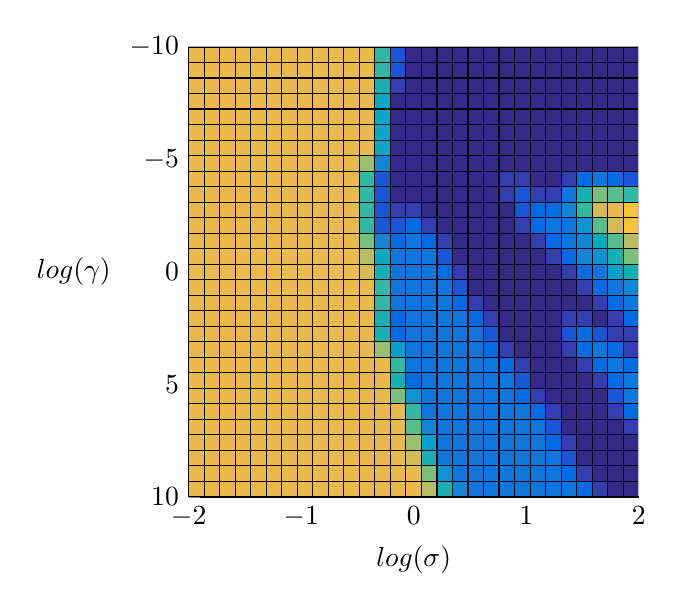
\begin{tikzpicture}

\begin{axis}[%
width=2.25in,
height=2.25in,
at={(0.631944in,0.48125in)},
scale only axis,
xmin=-10,
xmax=10,
xlabel={$log(\gamma)$},
xmajorgrids,
ymin=-2,
ymax=2,
ylabel={$log(\sigma)$},
ymajorgrids,
zmin=0,
zmax=0.5,
zmajorgrids,
view={90}{90},
axis x line*=bottom,
axis y line*=left,
axis z line*=left
]

\addplot3[%
surf,
faceted color=black,
shader=faceted,
colormap={mymap}{[1pt] rgb(0pt)=(0.2081,0.1663,0.5292); rgb(1pt)=(0.211624,0.189781,0.577676); rgb(2pt)=(0.212252,0.213771,0.626971); rgb(3pt)=(0.2081,0.2386,0.677086); rgb(4pt)=(0.195905,0.264457,0.7279); rgb(5pt)=(0.170729,0.291938,0.779248); rgb(6pt)=(0.125271,0.324243,0.830271); rgb(7pt)=(0.0591333,0.359833,0.868333); rgb(8pt)=(0.0116952,0.38751,0.881957); rgb(9pt)=(0.00595714,0.408614,0.882843); rgb(10pt)=(0.0165143,0.4266,0.878633); rgb(11pt)=(0.0328524,0.443043,0.871957); rgb(12pt)=(0.0498143,0.458571,0.864057); rgb(13pt)=(0.0629333,0.47369,0.855438); rgb(14pt)=(0.0722667,0.488667,0.8467); rgb(15pt)=(0.0779429,0.503986,0.838371); rgb(16pt)=(0.0793476,0.520024,0.831181); rgb(17pt)=(0.0749429,0.537543,0.826271); rgb(18pt)=(0.0640571,0.556986,0.823957); rgb(19pt)=(0.0487714,0.577224,0.822829); rgb(20pt)=(0.0343429,0.596581,0.819852); rgb(21pt)=(0.0265,0.6137,0.8135); rgb(22pt)=(0.0238905,0.628662,0.803762); rgb(23pt)=(0.0230905,0.641786,0.791267); rgb(24pt)=(0.0227714,0.653486,0.776757); rgb(25pt)=(0.0266619,0.664195,0.760719); rgb(26pt)=(0.0383714,0.674271,0.743552); rgb(27pt)=(0.0589714,0.683757,0.725386); rgb(28pt)=(0.0843,0.692833,0.706167); rgb(29pt)=(0.113295,0.7015,0.685857); rgb(30pt)=(0.145271,0.709757,0.664629); rgb(31pt)=(0.180133,0.717657,0.642433); rgb(32pt)=(0.217829,0.725043,0.619262); rgb(33pt)=(0.258643,0.731714,0.595429); rgb(34pt)=(0.302171,0.737605,0.571186); rgb(35pt)=(0.348167,0.742433,0.547267); rgb(36pt)=(0.395257,0.7459,0.524443); rgb(37pt)=(0.44201,0.748081,0.503314); rgb(38pt)=(0.487124,0.749062,0.483976); rgb(39pt)=(0.530029,0.749114,0.466114); rgb(40pt)=(0.570857,0.748519,0.44939); rgb(41pt)=(0.609852,0.747314,0.433686); rgb(42pt)=(0.6473,0.7456,0.4188); rgb(43pt)=(0.683419,0.743476,0.404433); rgb(44pt)=(0.71841,0.741133,0.390476); rgb(45pt)=(0.752486,0.7384,0.376814); rgb(46pt)=(0.785843,0.735567,0.363271); rgb(47pt)=(0.818505,0.732733,0.34979); rgb(48pt)=(0.850657,0.7299,0.336029); rgb(49pt)=(0.882433,0.727433,0.3217); rgb(50pt)=(0.913933,0.725786,0.306276); rgb(51pt)=(0.944957,0.726114,0.288643); rgb(52pt)=(0.973895,0.731395,0.266648); rgb(53pt)=(0.993771,0.745457,0.240348); rgb(54pt)=(0.999043,0.765314,0.216414); rgb(55pt)=(0.995533,0.786057,0.196652); rgb(56pt)=(0.988,0.8066,0.179367); rgb(57pt)=(0.978857,0.827143,0.163314); rgb(58pt)=(0.9697,0.848138,0.147452); rgb(59pt)=(0.962586,0.870514,0.1309); rgb(60pt)=(0.958871,0.8949,0.113243); rgb(61pt)=(0.959824,0.921833,0.0948381); rgb(62pt)=(0.9661,0.951443,0.0755333); rgb(63pt)=(0.9763,0.9831,0.0538)},
mesh/rows=30]
table[row sep=crcr,header=false] {%
%
-10	-2	0.4\\
-10	-1.86206896551724	0.4\\
-10	-1.72413793103448	0.4\\
-10	-1.58620689655172	0.4\\
-10	-1.44827586206897	0.4\\
-10	-1.31034482758621	0.4\\
-10	-1.17241379310345	0.4\\
-10	-1.03448275862069	0.4\\
-10	-0.896551724137931	0.4\\
-10	-0.758620689655172	0.4\\
-10	-0.620689655172414	0.4\\
-10	-0.482758620689655	0.4\\
-10	-0.344827586206897	0.4\\
-10	-0.206896551724138	0.1\\
-10	-0.0689655172413792	0\\
-10	0.0689655172413794	0\\
-10	0.206896551724138	0\\
-10	0.344827586206896	0\\
-10	0.482758620689655	0\\
-10	0.620689655172414	0\\
-10	0.758620689655173	0\\
-10	0.896551724137931	0\\
-10	1.03448275862069	0\\
-10	1.17241379310345	0\\
-10	1.31034482758621	0\\
-10	1.44827586206897	0\\
-10	1.58620689655172	0\\
-10	1.72413793103448	0\\
-10	1.86206896551724	0\\
-10	2	0\\
-9.31034482758621	-2	0.4\\
-9.31034482758621	-1.86206896551724	0.4\\
-9.31034482758621	-1.72413793103448	0.4\\
-9.31034482758621	-1.58620689655172	0.4\\
-9.31034482758621	-1.44827586206897	0.4\\
-9.31034482758621	-1.31034482758621	0.4\\
-9.31034482758621	-1.17241379310345	0.4\\
-9.31034482758621	-1.03448275862069	0.4\\
-9.31034482758621	-0.896551724137931	0.4\\
-9.31034482758621	-0.758620689655172	0.4\\
-9.31034482758621	-0.620689655172414	0.4\\
-9.31034482758621	-0.482758620689655	0.4\\
-9.31034482758621	-0.344827586206897	0.4\\
-9.31034482758621	-0.206896551724138	0.1\\
-9.31034482758621	-0.0689655172413792	0\\
-9.31034482758621	0.0689655172413794	0\\
-9.31034482758621	0.206896551724138	0\\
-9.31034482758621	0.344827586206896	0\\
-9.31034482758621	0.482758620689655	0\\
-9.31034482758621	0.620689655172414	0\\
-9.31034482758621	0.758620689655173	0\\
-9.31034482758621	0.896551724137931	0\\
-9.31034482758621	1.03448275862069	0\\
-9.31034482758621	1.17241379310345	0\\
-9.31034482758621	1.31034482758621	0\\
-9.31034482758621	1.44827586206897	0\\
-9.31034482758621	1.58620689655172	0\\
-9.31034482758621	1.72413793103448	0\\
-9.31034482758621	1.86206896551724	0\\
-9.31034482758621	2	0\\
-8.62068965517241	-2	0.4\\
-8.62068965517241	-1.86206896551724	0.4\\
-8.62068965517241	-1.72413793103448	0.4\\
-8.62068965517241	-1.58620689655172	0.4\\
-8.62068965517241	-1.44827586206897	0.4\\
-8.62068965517241	-1.31034482758621	0.4\\
-8.62068965517241	-1.17241379310345	0.4\\
-8.62068965517241	-1.03448275862069	0.4\\
-8.62068965517241	-0.896551724137931	0.4\\
-8.62068965517241	-0.758620689655172	0.4\\
-8.62068965517241	-0.620689655172414	0.4\\
-8.62068965517241	-0.482758620689655	0.4\\
-8.62068965517241	-0.344827586206897	0.4\\
-8.62068965517241	-0.206896551724138	0.1\\
-8.62068965517241	-0.0689655172413792	0\\
-8.62068965517241	0.0689655172413794	0\\
-8.62068965517241	0.206896551724138	0\\
-8.62068965517241	0.344827586206896	0\\
-8.62068965517241	0.482758620689655	0\\
-8.62068965517241	0.620689655172414	0\\
-8.62068965517241	0.758620689655173	0\\
-8.62068965517241	0.896551724137931	0\\
-8.62068965517241	1.03448275862069	0\\
-8.62068965517241	1.17241379310345	0\\
-8.62068965517241	1.31034482758621	0\\
-8.62068965517241	1.44827586206897	0\\
-8.62068965517241	1.58620689655172	0\\
-8.62068965517241	1.72413793103448	0\\
-8.62068965517241	1.86206896551724	0\\
-8.62068965517241	2	0\\
-7.93103448275862	-2	0.4\\
-7.93103448275862	-1.86206896551724	0.4\\
-7.93103448275862	-1.72413793103448	0.4\\
-7.93103448275862	-1.58620689655172	0.4\\
-7.93103448275862	-1.44827586206897	0.4\\
-7.93103448275862	-1.31034482758621	0.4\\
-7.93103448275862	-1.17241379310345	0.4\\
-7.93103448275862	-1.03448275862069	0.4\\
-7.93103448275862	-0.896551724137931	0.4\\
-7.93103448275862	-0.758620689655172	0.4\\
-7.93103448275862	-0.620689655172414	0.4\\
-7.93103448275862	-0.482758620689655	0.4\\
-7.93103448275862	-0.344827586206897	0.4\\
-7.93103448275862	-0.206896551724138	0\\
-7.93103448275862	-0.0689655172413792	0\\
-7.93103448275862	0.0689655172413794	0\\
-7.93103448275862	0.206896551724138	0\\
-7.93103448275862	0.344827586206896	0\\
-7.93103448275862	0.482758620689655	0\\
-7.93103448275862	0.620689655172414	0\\
-7.93103448275862	0.758620689655173	0\\
-7.93103448275862	0.896551724137931	0\\
-7.93103448275862	1.03448275862069	0\\
-7.93103448275862	1.17241379310345	0\\
-7.93103448275862	1.31034482758621	0\\
-7.93103448275862	1.44827586206897	0\\
-7.93103448275862	1.58620689655172	0\\
-7.93103448275862	1.72413793103448	0\\
-7.93103448275862	1.86206896551724	0\\
-7.93103448275862	2	0\\
-7.24137931034483	-2	0.4\\
-7.24137931034483	-1.86206896551724	0.4\\
-7.24137931034483	-1.72413793103448	0.4\\
-7.24137931034483	-1.58620689655172	0.4\\
-7.24137931034483	-1.44827586206897	0.4\\
-7.24137931034483	-1.31034482758621	0.4\\
-7.24137931034483	-1.17241379310345	0.4\\
-7.24137931034483	-1.03448275862069	0.4\\
-7.24137931034483	-0.896551724137931	0.4\\
-7.24137931034483	-0.758620689655172	0.4\\
-7.24137931034483	-0.620689655172414	0.4\\
-7.24137931034483	-0.482758620689655	0.4\\
-7.24137931034483	-0.344827586206897	0.4\\
-7.24137931034483	-0.206896551724138	0\\
-7.24137931034483	-0.0689655172413792	0\\
-7.24137931034483	0.0689655172413794	0\\
-7.24137931034483	0.206896551724138	0\\
-7.24137931034483	0.344827586206896	0\\
-7.24137931034483	0.482758620689655	0\\
-7.24137931034483	0.620689655172414	0\\
-7.24137931034483	0.758620689655173	0\\
-7.24137931034483	0.896551724137931	0\\
-7.24137931034483	1.03448275862069	0\\
-7.24137931034483	1.17241379310345	0\\
-7.24137931034483	1.31034482758621	0\\
-7.24137931034483	1.44827586206897	0\\
-7.24137931034483	1.58620689655172	0\\
-7.24137931034483	1.72413793103448	0\\
-7.24137931034483	1.86206896551724	0\\
-7.24137931034483	2	0\\
-6.55172413793103	-2	0.4\\
-6.55172413793103	-1.86206896551724	0.4\\
-6.55172413793103	-1.72413793103448	0.4\\
-6.55172413793103	-1.58620689655172	0.4\\
-6.55172413793103	-1.44827586206897	0.4\\
-6.55172413793103	-1.31034482758621	0.4\\
-6.55172413793103	-1.17241379310345	0.4\\
-6.55172413793103	-1.03448275862069	0.4\\
-6.55172413793103	-0.896551724137931	0.4\\
-6.55172413793103	-0.758620689655172	0.4\\
-6.55172413793103	-0.620689655172414	0.4\\
-6.55172413793103	-0.482758620689655	0.4\\
-6.55172413793103	-0.344827586206897	0.4\\
-6.55172413793103	-0.206896551724138	0\\
-6.55172413793103	-0.0689655172413792	0\\
-6.55172413793103	0.0689655172413794	0\\
-6.55172413793103	0.206896551724138	0\\
-6.55172413793103	0.344827586206896	0\\
-6.55172413793103	0.482758620689655	0\\
-6.55172413793103	0.620689655172414	0\\
-6.55172413793103	0.758620689655173	0\\
-6.55172413793103	0.896551724137931	0\\
-6.55172413793103	1.03448275862069	0\\
-6.55172413793103	1.17241379310345	0\\
-6.55172413793103	1.31034482758621	0\\
-6.55172413793103	1.44827586206897	0\\
-6.55172413793103	1.58620689655172	0\\
-6.55172413793103	1.72413793103448	0\\
-6.55172413793103	1.86206896551724	0\\
-6.55172413793103	2	0\\
-5.86206896551724	-2	0.4\\
-5.86206896551724	-1.86206896551724	0.4\\
-5.86206896551724	-1.72413793103448	0.4\\
-5.86206896551724	-1.58620689655172	0.4\\
-5.86206896551724	-1.44827586206897	0.4\\
-5.86206896551724	-1.31034482758621	0.4\\
-5.86206896551724	-1.17241379310345	0.4\\
-5.86206896551724	-1.03448275862069	0.4\\
-5.86206896551724	-0.896551724137931	0.4\\
-5.86206896551724	-0.758620689655172	0.4\\
-5.86206896551724	-0.620689655172414	0.4\\
-5.86206896551724	-0.482758620689655	0.4\\
-5.86206896551724	-0.344827586206897	0.4\\
-5.86206896551724	-0.206896551724138	0\\
-5.86206896551724	-0.0689655172413792	0\\
-5.86206896551724	0.0689655172413794	0\\
-5.86206896551724	0.206896551724138	0\\
-5.86206896551724	0.344827586206896	0\\
-5.86206896551724	0.482758620689655	0\\
-5.86206896551724	0.620689655172414	0\\
-5.86206896551724	0.758620689655173	0\\
-5.86206896551724	0.896551724137931	0\\
-5.86206896551724	1.03448275862069	0\\
-5.86206896551724	1.17241379310345	0\\
-5.86206896551724	1.31034482758621	0\\
-5.86206896551724	1.44827586206897	0\\
-5.86206896551724	1.58620689655172	0\\
-5.86206896551724	1.72413793103448	0\\
-5.86206896551724	1.86206896551724	0\\
-5.86206896551724	2	0\\
-5.17241379310345	-2	0.4\\
-5.17241379310345	-1.86206896551724	0.4\\
-5.17241379310345	-1.72413793103448	0.4\\
-5.17241379310345	-1.58620689655172	0.4\\
-5.17241379310345	-1.44827586206897	0.4\\
-5.17241379310345	-1.31034482758621	0.4\\
-5.17241379310345	-1.17241379310345	0.4\\
-5.17241379310345	-1.03448275862069	0.4\\
-5.17241379310345	-0.896551724137931	0.4\\
-5.17241379310345	-0.758620689655172	0.4\\
-5.17241379310345	-0.620689655172414	0.4\\
-5.17241379310345	-0.482758620689655	0.4\\
-5.17241379310345	-0.344827586206897	0.4\\
-5.17241379310345	-0.206896551724138	0\\
-5.17241379310345	-0.0689655172413792	0\\
-5.17241379310345	0.0689655172413794	0\\
-5.17241379310345	0.206896551724138	0\\
-5.17241379310345	0.344827586206896	0\\
-5.17241379310345	0.482758620689655	0\\
-5.17241379310345	0.620689655172414	0\\
-5.17241379310345	0.758620689655173	0\\
-5.17241379310345	0.896551724137931	0\\
-5.17241379310345	1.03448275862069	0\\
-5.17241379310345	1.17241379310345	0\\
-5.17241379310345	1.31034482758621	0\\
-5.17241379310345	1.44827586206897	0\\
-5.17241379310345	1.58620689655172	0\\
-5.17241379310345	1.72413793103448	0\\
-5.17241379310345	1.86206896551724	0\\
-5.17241379310345	2	0\\
-4.48275862068965	-2	0.4\\
-4.48275862068965	-1.86206896551724	0.4\\
-4.48275862068965	-1.72413793103448	0.4\\
-4.48275862068965	-1.58620689655172	0.4\\
-4.48275862068965	-1.44827586206897	0.4\\
-4.48275862068965	-1.31034482758621	0.4\\
-4.48275862068965	-1.17241379310345	0.4\\
-4.48275862068965	-1.03448275862069	0.4\\
-4.48275862068965	-0.896551724137931	0.4\\
-4.48275862068965	-0.758620689655172	0.4\\
-4.48275862068965	-0.620689655172414	0.4\\
-4.48275862068965	-0.482758620689655	0.4\\
-4.48275862068965	-0.344827586206897	0.1\\
-4.48275862068965	-0.206896551724138	0\\
-4.48275862068965	-0.0689655172413792	0\\
-4.48275862068965	0.0689655172413794	0\\
-4.48275862068965	0.206896551724138	0\\
-4.48275862068965	0.344827586206896	0\\
-4.48275862068965	0.482758620689655	0\\
-4.48275862068965	0.620689655172414	0\\
-4.48275862068965	0.758620689655173	0\\
-4.48275862068965	0.896551724137931	0\\
-4.48275862068965	1.03448275862069	0\\
-4.48275862068965	1.17241379310345	0\\
-4.48275862068965	1.31034482758621	0\\
-4.48275862068965	1.44827586206897	0\\
-4.48275862068965	1.58620689655172	0\\
-4.48275862068965	1.72413793103448	0\\
-4.48275862068965	1.86206896551724	0\\
-4.48275862068965	2	0\\
-3.79310344827586	-2	0.4\\
-3.79310344827586	-1.86206896551724	0.4\\
-3.79310344827586	-1.72413793103448	0.4\\
-3.79310344827586	-1.58620689655172	0.4\\
-3.79310344827586	-1.44827586206897	0.4\\
-3.79310344827586	-1.31034482758621	0.4\\
-3.79310344827586	-1.17241379310345	0.4\\
-3.79310344827586	-1.03448275862069	0.4\\
-3.79310344827586	-0.896551724137931	0.4\\
-3.79310344827586	-0.758620689655172	0.4\\
-3.79310344827586	-0.620689655172414	0.4\\
-3.79310344827586	-0.482758620689655	0.4\\
-3.79310344827586	-0.344827586206897	0.1\\
-3.79310344827586	-0.206896551724138	0\\
-3.79310344827586	-0.0689655172413792	0\\
-3.79310344827586	0.0689655172413794	0\\
-3.79310344827586	0.206896551724138	0\\
-3.79310344827586	0.344827586206896	0\\
-3.79310344827586	0.482758620689655	0\\
-3.79310344827586	0.620689655172414	0\\
-3.79310344827586	0.758620689655173	0\\
-3.79310344827586	0.896551724137931	0.1\\
-3.79310344827586	1.03448275862069	0\\
-3.79310344827586	1.17241379310345	0\\
-3.79310344827586	1.31034482758621	0\\
-3.79310344827586	1.44827586206897	0.1\\
-3.79310344827586	1.58620689655172	0.2\\
-3.79310344827586	1.72413793103448	0.2\\
-3.79310344827586	1.86206896551724	0.1\\
-3.79310344827586	2	0.1\\
-3.10344827586207	-2	0.4\\
-3.10344827586207	-1.86206896551724	0.4\\
-3.10344827586207	-1.72413793103448	0.4\\
-3.10344827586207	-1.58620689655172	0.4\\
-3.10344827586207	-1.44827586206897	0.4\\
-3.10344827586207	-1.31034482758621	0.4\\
-3.10344827586207	-1.17241379310345	0.4\\
-3.10344827586207	-1.03448275862069	0.4\\
-3.10344827586207	-0.896551724137931	0.4\\
-3.10344827586207	-0.758620689655172	0.4\\
-3.10344827586207	-0.620689655172414	0.4\\
-3.10344827586207	-0.482758620689655	0.4\\
-3.10344827586207	-0.344827586206897	0.1\\
-3.10344827586207	-0.206896551724138	0\\
-3.10344827586207	-0.0689655172413792	0\\
-3.10344827586207	0.0689655172413794	0\\
-3.10344827586207	0.206896551724138	0\\
-3.10344827586207	0.344827586206896	0\\
-3.10344827586207	0.482758620689655	0\\
-3.10344827586207	0.620689655172414	0\\
-3.10344827586207	0.758620689655173	0\\
-3.10344827586207	0.896551724137931	0\\
-3.10344827586207	1.03448275862069	0.1\\
-3.10344827586207	1.17241379310345	0\\
-3.10344827586207	1.31034482758621	0.1\\
-3.10344827586207	1.44827586206897	0.2\\
-3.10344827586207	1.58620689655172	0.4\\
-3.10344827586207	1.72413793103448	0.4\\
-3.10344827586207	1.86206896551724	0.4\\
-3.10344827586207	2	0.4\\
-2.41379310344828	-2	0.4\\
-2.41379310344828	-1.86206896551724	0.4\\
-2.41379310344828	-1.72413793103448	0.4\\
-2.41379310344828	-1.58620689655172	0.4\\
-2.41379310344828	-1.44827586206897	0.4\\
-2.41379310344828	-1.31034482758621	0.4\\
-2.41379310344828	-1.17241379310345	0.4\\
-2.41379310344828	-1.03448275862069	0.4\\
-2.41379310344828	-0.896551724137931	0.4\\
-2.41379310344828	-0.758620689655172	0.4\\
-2.41379310344828	-0.620689655172414	0.4\\
-2.41379310344828	-0.482758620689655	0.4\\
-2.41379310344828	-0.344827586206897	0.1\\
-2.41379310344828	-0.206896551724138	0\\
-2.41379310344828	-0.0689655172413792	0.1\\
-2.41379310344828	0.0689655172413794	0\\
-2.41379310344828	0.206896551724138	0\\
-2.41379310344828	0.344827586206896	0\\
-2.41379310344828	0.482758620689655	0\\
-2.41379310344828	0.620689655172414	0\\
-2.41379310344828	0.758620689655173	0\\
-2.41379310344828	0.896551724137931	0\\
-2.41379310344828	1.03448275862069	0.1\\
-2.41379310344828	1.17241379310345	0.1\\
-2.41379310344828	1.31034482758621	0.1\\
-2.41379310344828	1.44827586206897	0.1\\
-2.41379310344828	1.58620689655172	0.3\\
-2.41379310344828	1.72413793103448	0.4\\
-2.41379310344828	1.86206896551724	0.4\\
-2.41379310344828	2	0.5\\
-1.72413793103448	-2	0.4\\
-1.72413793103448	-1.86206896551724	0.4\\
-1.72413793103448	-1.72413793103448	0.4\\
-1.72413793103448	-1.58620689655172	0.4\\
-1.72413793103448	-1.44827586206897	0.4\\
-1.72413793103448	-1.31034482758621	0.4\\
-1.72413793103448	-1.17241379310345	0.4\\
-1.72413793103448	-1.03448275862069	0.4\\
-1.72413793103448	-0.896551724137931	0.4\\
-1.72413793103448	-0.758620689655172	0.4\\
-1.72413793103448	-0.620689655172414	0.4\\
-1.72413793103448	-0.482758620689655	0.4\\
-1.72413793103448	-0.344827586206897	0.1\\
-1.72413793103448	-0.206896551724138	0\\
-1.72413793103448	-0.0689655172413792	0.1\\
-1.72413793103448	0.0689655172413794	0.1\\
-1.72413793103448	0.206896551724138	0\\
-1.72413793103448	0.344827586206896	0\\
-1.72413793103448	0.482758620689655	0\\
-1.72413793103448	0.620689655172414	0\\
-1.72413793103448	0.758620689655173	0\\
-1.72413793103448	0.896551724137931	0\\
-1.72413793103448	1.03448275862069	0\\
-1.72413793103448	1.17241379310345	0.1\\
-1.72413793103448	1.31034482758621	0.1\\
-1.72413793103448	1.44827586206897	0.1\\
-1.72413793103448	1.58620689655172	0.1\\
-1.72413793103448	1.72413793103448	0.3\\
-1.72413793103448	1.86206896551724	0.4\\
-1.72413793103448	2	0.4\\
-1.03448275862069	-2	0.4\\
-1.03448275862069	-1.86206896551724	0.4\\
-1.03448275862069	-1.72413793103448	0.4\\
-1.03448275862069	-1.58620689655172	0.4\\
-1.03448275862069	-1.44827586206897	0.4\\
-1.03448275862069	-1.31034482758621	0.4\\
-1.03448275862069	-1.17241379310345	0.4\\
-1.03448275862069	-1.03448275862069	0.4\\
-1.03448275862069	-0.896551724137931	0.4\\
-1.03448275862069	-0.758620689655172	0.4\\
-1.03448275862069	-0.620689655172414	0.4\\
-1.03448275862069	-0.482758620689655	0.4\\
-1.03448275862069	-0.344827586206897	0.3\\
-1.03448275862069	-0.206896551724138	0.1\\
-1.03448275862069	-0.0689655172413792	0.1\\
-1.03448275862069	0.0689655172413794	0.1\\
-1.03448275862069	0.206896551724138	0.1\\
-1.03448275862069	0.344827586206896	0\\
-1.03448275862069	0.482758620689655	0\\
-1.03448275862069	0.620689655172414	0\\
-1.03448275862069	0.758620689655173	0\\
-1.03448275862069	0.896551724137931	0\\
-1.03448275862069	1.03448275862069	0\\
-1.03448275862069	1.17241379310345	0\\
-1.03448275862069	1.31034482758621	0.1\\
-1.03448275862069	1.44827586206897	0.1\\
-1.03448275862069	1.58620689655172	0.2\\
-1.03448275862069	1.72413793103448	0.2\\
-1.03448275862069	1.86206896551724	0.2\\
-1.03448275862069	2	0.4\\
-0.344827586206897	-2	0.4\\
-0.344827586206897	-1.86206896551724	0.4\\
-0.344827586206897	-1.72413793103448	0.4\\
-0.344827586206897	-1.58620689655172	0.4\\
-0.344827586206897	-1.44827586206897	0.4\\
-0.344827586206897	-1.31034482758621	0.4\\
-0.344827586206897	-1.17241379310345	0.4\\
-0.344827586206897	-1.03448275862069	0.4\\
-0.344827586206897	-0.896551724137931	0.4\\
-0.344827586206897	-0.758620689655172	0.4\\
-0.344827586206897	-0.620689655172414	0.4\\
-0.344827586206897	-0.482758620689655	0.4\\
-0.344827586206897	-0.344827586206897	0.3\\
-0.344827586206897	-0.206896551724138	0.1\\
-0.344827586206897	-0.0689655172413792	0.1\\
-0.344827586206897	0.0689655172413794	0.1\\
-0.344827586206897	0.206896551724138	0.1\\
-0.344827586206897	0.344827586206896	0\\
-0.344827586206897	0.482758620689655	0\\
-0.344827586206897	0.620689655172414	0\\
-0.344827586206897	0.758620689655173	0\\
-0.344827586206897	0.896551724137931	0\\
-0.344827586206897	1.03448275862069	0\\
-0.344827586206897	1.17241379310345	0\\
-0.344827586206897	1.31034482758621	0\\
-0.344827586206897	1.44827586206897	0.1\\
-0.344827586206897	1.58620689655172	0.1\\
-0.344827586206897	1.72413793103448	0.1\\
-0.344827586206897	1.86206896551724	0.4\\
-0.344827586206897	2	0.2\\
0.344827586206897	-2	0.4\\
0.344827586206897	-1.86206896551724	0.4\\
0.344827586206897	-1.72413793103448	0.4\\
0.344827586206897	-1.58620689655172	0.4\\
0.344827586206897	-1.44827586206897	0.4\\
0.344827586206897	-1.31034482758621	0.4\\
0.344827586206897	-1.17241379310345	0.4\\
0.344827586206897	-1.03448275862069	0.4\\
0.344827586206897	-0.896551724137931	0.4\\
0.344827586206897	-0.758620689655172	0.4\\
0.344827586206897	-0.620689655172414	0.4\\
0.344827586206897	-0.482758620689655	0.4\\
0.344827586206897	-0.344827586206897	0.4\\
0.344827586206897	-0.206896551724138	0.1\\
0.344827586206897	-0.0689655172413792	0.1\\
0.344827586206897	0.0689655172413794	0.1\\
0.344827586206897	0.206896551724138	0.1\\
0.344827586206897	0.344827586206896	0.1\\
0.344827586206897	0.482758620689655	0\\
0.344827586206897	0.620689655172414	0\\
0.344827586206897	0.758620689655173	0\\
0.344827586206897	0.896551724137931	0\\
0.344827586206897	1.03448275862069	0\\
0.344827586206897	1.17241379310345	0\\
0.344827586206897	1.31034482758621	0\\
0.344827586206897	1.44827586206897	0\\
0.344827586206897	1.58620689655172	0.1\\
0.344827586206897	1.72413793103448	0.1\\
0.344827586206897	1.86206896551724	0.1\\
0.344827586206897	2	0.2\\
1.03448275862069	-2	0.4\\
1.03448275862069	-1.86206896551724	0.4\\
1.03448275862069	-1.72413793103448	0.4\\
1.03448275862069	-1.58620689655172	0.4\\
1.03448275862069	-1.44827586206897	0.4\\
1.03448275862069	-1.31034482758621	0.4\\
1.03448275862069	-1.17241379310345	0.4\\
1.03448275862069	-1.03448275862069	0.4\\
1.03448275862069	-0.896551724137931	0.4\\
1.03448275862069	-0.758620689655172	0.4\\
1.03448275862069	-0.620689655172414	0.4\\
1.03448275862069	-0.482758620689655	0.4\\
1.03448275862069	-0.344827586206897	0.4\\
1.03448275862069	-0.206896551724138	0.1\\
1.03448275862069	-0.0689655172413792	0.1\\
1.03448275862069	0.0689655172413794	0.1\\
1.03448275862069	0.206896551724138	0.1\\
1.03448275862069	0.344827586206896	0.1\\
1.03448275862069	0.482758620689655	0\\
1.03448275862069	0.620689655172414	0\\
1.03448275862069	0.758620689655173	0\\
1.03448275862069	0.896551724137931	0\\
1.03448275862069	1.03448275862069	0\\
1.03448275862069	1.17241379310345	0\\
1.03448275862069	1.31034482758621	0\\
1.03448275862069	1.44827586206897	0\\
1.03448275862069	1.58620689655172	0\\
1.03448275862069	1.72413793103448	0.1\\
1.03448275862069	1.86206896551724	0.1\\
1.03448275862069	2	0.1\\
1.72413793103448	-2	0.4\\
1.72413793103448	-1.86206896551724	0.4\\
1.72413793103448	-1.72413793103448	0.4\\
1.72413793103448	-1.58620689655172	0.4\\
1.72413793103448	-1.44827586206897	0.4\\
1.72413793103448	-1.31034482758621	0.4\\
1.72413793103448	-1.17241379310345	0.4\\
1.72413793103448	-1.03448275862069	0.4\\
1.72413793103448	-0.896551724137931	0.4\\
1.72413793103448	-0.758620689655172	0.4\\
1.72413793103448	-0.620689655172414	0.4\\
1.72413793103448	-0.482758620689655	0.4\\
1.72413793103448	-0.344827586206897	0.4\\
1.72413793103448	-0.206896551724138	0.1\\
1.72413793103448	-0.0689655172413792	0.1\\
1.72413793103448	0.0689655172413794	0.1\\
1.72413793103448	0.206896551724138	0.1\\
1.72413793103448	0.344827586206896	0.1\\
1.72413793103448	0.482758620689655	0.1\\
1.72413793103448	0.620689655172414	0\\
1.72413793103448	0.758620689655173	0\\
1.72413793103448	0.896551724137931	0\\
1.72413793103448	1.03448275862069	0\\
1.72413793103448	1.17241379310345	0\\
1.72413793103448	1.31034482758621	0\\
1.72413793103448	1.44827586206897	0\\
1.72413793103448	1.58620689655172	0\\
1.72413793103448	1.72413793103448	0\\
1.72413793103448	1.86206896551724	0.1\\
1.72413793103448	2	0.1\\
2.41379310344828	-2	0.4\\
2.41379310344828	-1.86206896551724	0.4\\
2.41379310344828	-1.72413793103448	0.4\\
2.41379310344828	-1.58620689655172	0.4\\
2.41379310344828	-1.44827586206897	0.4\\
2.41379310344828	-1.31034482758621	0.4\\
2.41379310344828	-1.17241379310345	0.4\\
2.41379310344828	-1.03448275862069	0.4\\
2.41379310344828	-0.896551724137931	0.4\\
2.41379310344828	-0.758620689655172	0.4\\
2.41379310344828	-0.620689655172414	0.4\\
2.41379310344828	-0.482758620689655	0.4\\
2.41379310344828	-0.344827586206897	0.4\\
2.41379310344828	-0.206896551724138	0\\
2.41379310344828	-0.0689655172413792	0.1\\
2.41379310344828	0.0689655172413794	0.1\\
2.41379310344828	0.206896551724138	0.1\\
2.41379310344828	0.344827586206896	0.1\\
2.41379310344828	0.482758620689655	0.1\\
2.41379310344828	0.620689655172414	0.1\\
2.41379310344828	0.758620689655173	0\\
2.41379310344828	0.896551724137931	0\\
2.41379310344828	1.03448275862069	0\\
2.41379310344828	1.17241379310345	0\\
2.41379310344828	1.31034482758621	0\\
2.41379310344828	1.44827586206897	0.1\\
2.41379310344828	1.58620689655172	0\\
2.41379310344828	1.72413793103448	0\\
2.41379310344828	1.86206896551724	0\\
2.41379310344828	2	0.1\\
3.10344827586207	-2	0.4\\
3.10344827586207	-1.86206896551724	0.4\\
3.10344827586207	-1.72413793103448	0.4\\
3.10344827586207	-1.58620689655172	0.4\\
3.10344827586207	-1.44827586206897	0.4\\
3.10344827586207	-1.31034482758621	0.4\\
3.10344827586207	-1.17241379310345	0.4\\
3.10344827586207	-1.03448275862069	0.4\\
3.10344827586207	-0.896551724137931	0.4\\
3.10344827586207	-0.758620689655172	0.4\\
3.10344827586207	-0.620689655172414	0.4\\
3.10344827586207	-0.482758620689655	0.4\\
3.10344827586207	-0.344827586206897	0.4\\
3.10344827586207	-0.206896551724138	0.1\\
3.10344827586207	-0.0689655172413792	0.1\\
3.10344827586207	0.0689655172413794	0.1\\
3.10344827586207	0.206896551724138	0.1\\
3.10344827586207	0.344827586206896	0.1\\
3.10344827586207	0.482758620689655	0.1\\
3.10344827586207	0.620689655172414	0.1\\
3.10344827586207	0.758620689655173	0\\
3.10344827586207	0.896551724137931	0\\
3.10344827586207	1.03448275862069	0\\
3.10344827586207	1.17241379310345	0\\
3.10344827586207	1.31034482758621	0\\
3.10344827586207	1.44827586206897	0.1\\
3.10344827586207	1.58620689655172	0.1\\
3.10344827586207	1.72413793103448	0.1\\
3.10344827586207	1.86206896551724	0\\
3.10344827586207	2	0\\
3.79310344827586	-2	0.4\\
3.79310344827586	-1.86206896551724	0.4\\
3.79310344827586	-1.72413793103448	0.4\\
3.79310344827586	-1.58620689655172	0.4\\
3.79310344827586	-1.44827586206897	0.4\\
3.79310344827586	-1.31034482758621	0.4\\
3.79310344827586	-1.17241379310345	0.4\\
3.79310344827586	-1.03448275862069	0.4\\
3.79310344827586	-0.896551724137931	0.4\\
3.79310344827586	-0.758620689655172	0.4\\
3.79310344827586	-0.620689655172414	0.4\\
3.79310344827586	-0.482758620689655	0.4\\
3.79310344827586	-0.344827586206897	0.4\\
3.79310344827586	-0.206896551724138	0.4\\
3.79310344827586	-0.0689655172413792	0.1\\
3.79310344827586	0.0689655172413794	0.1\\
3.79310344827586	0.206896551724138	0.1\\
3.79310344827586	0.344827586206896	0.1\\
3.79310344827586	0.482758620689655	0.1\\
3.79310344827586	0.620689655172414	0.1\\
3.79310344827586	0.758620689655173	0.1\\
3.79310344827586	0.896551724137931	0\\
3.79310344827586	1.03448275862069	0\\
3.79310344827586	1.17241379310345	0\\
3.79310344827586	1.31034482758621	0\\
3.79310344827586	1.44827586206897	0\\
3.79310344827586	1.58620689655172	0.1\\
3.79310344827586	1.72413793103448	0.1\\
3.79310344827586	1.86206896551724	0.1\\
3.79310344827586	2	0\\
4.48275862068965	-2	0.4\\
4.48275862068965	-1.86206896551724	0.4\\
4.48275862068965	-1.72413793103448	0.4\\
4.48275862068965	-1.58620689655172	0.4\\
4.48275862068965	-1.44827586206897	0.4\\
4.48275862068965	-1.31034482758621	0.4\\
4.48275862068965	-1.17241379310345	0.4\\
4.48275862068965	-1.03448275862069	0.4\\
4.48275862068965	-0.896551724137931	0.4\\
4.48275862068965	-0.758620689655172	0.4\\
4.48275862068965	-0.620689655172414	0.4\\
4.48275862068965	-0.482758620689655	0.4\\
4.48275862068965	-0.344827586206897	0.4\\
4.48275862068965	-0.206896551724138	0.4\\
4.48275862068965	-0.0689655172413792	0.1\\
4.48275862068965	0.0689655172413794	0.1\\
4.48275862068965	0.206896551724138	0.1\\
4.48275862068965	0.344827586206896	0.1\\
4.48275862068965	0.482758620689655	0.1\\
4.48275862068965	0.620689655172414	0.1\\
4.48275862068965	0.758620689655173	0.1\\
4.48275862068965	0.896551724137931	0.1\\
4.48275862068965	1.03448275862069	0\\
4.48275862068965	1.17241379310345	0\\
4.48275862068965	1.31034482758621	0\\
4.48275862068965	1.44827586206897	0\\
4.48275862068965	1.58620689655172	0\\
4.48275862068965	1.72413793103448	0.1\\
4.48275862068965	1.86206896551724	0.1\\
4.48275862068965	2	0.1\\
5.17241379310345	-2	0.4\\
5.17241379310345	-1.86206896551724	0.4\\
5.17241379310345	-1.72413793103448	0.4\\
5.17241379310345	-1.58620689655172	0.4\\
5.17241379310345	-1.44827586206897	0.4\\
5.17241379310345	-1.31034482758621	0.4\\
5.17241379310345	-1.17241379310345	0.4\\
5.17241379310345	-1.03448275862069	0.4\\
5.17241379310345	-0.896551724137931	0.4\\
5.17241379310345	-0.758620689655172	0.4\\
5.17241379310345	-0.620689655172414	0.4\\
5.17241379310345	-0.482758620689655	0.4\\
5.17241379310345	-0.344827586206897	0.4\\
5.17241379310345	-0.206896551724138	0.4\\
5.17241379310345	-0.0689655172413792	0\\
5.17241379310345	0.0689655172413794	0.1\\
5.17241379310345	0.206896551724138	0.1\\
5.17241379310345	0.344827586206896	0.1\\
5.17241379310345	0.482758620689655	0.1\\
5.17241379310345	0.620689655172414	0.1\\
5.17241379310345	0.758620689655173	0.1\\
5.17241379310345	0.896551724137931	0.1\\
5.17241379310345	1.03448275862069	0\\
5.17241379310345	1.17241379310345	0\\
5.17241379310345	1.31034482758621	0\\
5.17241379310345	1.44827586206897	0\\
5.17241379310345	1.58620689655172	0\\
5.17241379310345	1.72413793103448	0\\
5.17241379310345	1.86206896551724	0.1\\
5.17241379310345	2	0.1\\
5.86206896551724	-2	0.4\\
5.86206896551724	-1.86206896551724	0.4\\
5.86206896551724	-1.72413793103448	0.4\\
5.86206896551724	-1.58620689655172	0.4\\
5.86206896551724	-1.44827586206897	0.4\\
5.86206896551724	-1.31034482758621	0.4\\
5.86206896551724	-1.17241379310345	0.4\\
5.86206896551724	-1.03448275862069	0.4\\
5.86206896551724	-0.896551724137931	0.4\\
5.86206896551724	-0.758620689655172	0.4\\
5.86206896551724	-0.620689655172414	0.4\\
5.86206896551724	-0.482758620689655	0.4\\
5.86206896551724	-0.344827586206897	0.4\\
5.86206896551724	-0.206896551724138	0.4\\
5.86206896551724	-0.0689655172413792	0.4\\
5.86206896551724	0.0689655172413794	0.1\\
5.86206896551724	0.206896551724138	0.1\\
5.86206896551724	0.344827586206896	0.1\\
5.86206896551724	0.482758620689655	0.1\\
5.86206896551724	0.620689655172414	0.1\\
5.86206896551724	0.758620689655173	0.1\\
5.86206896551724	0.896551724137931	0.1\\
5.86206896551724	1.03448275862069	0.1\\
5.86206896551724	1.17241379310345	0\\
5.86206896551724	1.31034482758621	0\\
5.86206896551724	1.44827586206897	0\\
5.86206896551724	1.58620689655172	0\\
5.86206896551724	1.72413793103448	0\\
5.86206896551724	1.86206896551724	0.1\\
5.86206896551724	2	0.1\\
6.55172413793104	-2	0.4\\
6.55172413793104	-1.86206896551724	0.4\\
6.55172413793104	-1.72413793103448	0.4\\
6.55172413793104	-1.58620689655172	0.4\\
6.55172413793104	-1.44827586206897	0.4\\
6.55172413793104	-1.31034482758621	0.4\\
6.55172413793104	-1.17241379310345	0.4\\
6.55172413793104	-1.03448275862069	0.4\\
6.55172413793104	-0.896551724137931	0.4\\
6.55172413793104	-0.758620689655172	0.4\\
6.55172413793104	-0.620689655172414	0.4\\
6.55172413793104	-0.482758620689655	0.4\\
6.55172413793104	-0.344827586206897	0.4\\
6.55172413793104	-0.206896551724138	0.4\\
6.55172413793104	-0.0689655172413792	0.4\\
6.55172413793104	0.0689655172413794	0.1\\
6.55172413793104	0.206896551724138	0.1\\
6.55172413793104	0.344827586206896	0.1\\
6.55172413793104	0.482758620689655	0.1\\
6.55172413793104	0.620689655172414	0.1\\
6.55172413793104	0.758620689655173	0.1\\
6.55172413793104	0.896551724137931	0.1\\
6.55172413793104	1.03448275862069	0.1\\
6.55172413793104	1.17241379310345	0.1\\
6.55172413793104	1.31034482758621	0\\
6.55172413793104	1.44827586206897	0\\
6.55172413793104	1.58620689655172	0\\
6.55172413793104	1.72413793103448	0\\
6.55172413793104	1.86206896551724	0\\
6.55172413793104	2	0.1\\
7.24137931034483	-2	0.4\\
7.24137931034483	-1.86206896551724	0.4\\
7.24137931034483	-1.72413793103448	0.4\\
7.24137931034483	-1.58620689655172	0.4\\
7.24137931034483	-1.44827586206897	0.4\\
7.24137931034483	-1.31034482758621	0.4\\
7.24137931034483	-1.17241379310345	0.4\\
7.24137931034483	-1.03448275862069	0.4\\
7.24137931034483	-0.896551724137931	0.4\\
7.24137931034483	-0.758620689655172	0.4\\
7.24137931034483	-0.620689655172414	0.4\\
7.24137931034483	-0.482758620689655	0.4\\
7.24137931034483	-0.344827586206897	0.4\\
7.24137931034483	-0.206896551724138	0.4\\
7.24137931034483	-0.0689655172413792	0.4\\
7.24137931034483	0.0689655172413794	0.2\\
7.24137931034483	0.206896551724138	0.1\\
7.24137931034483	0.344827586206896	0.1\\
7.24137931034483	0.482758620689655	0.1\\
7.24137931034483	0.620689655172414	0.1\\
7.24137931034483	0.758620689655173	0.1\\
7.24137931034483	0.896551724137931	0.1\\
7.24137931034483	1.03448275862069	0.1\\
7.24137931034483	1.17241379310345	0.1\\
7.24137931034483	1.31034482758621	0\\
7.24137931034483	1.44827586206897	0\\
7.24137931034483	1.58620689655172	0\\
7.24137931034483	1.72413793103448	0\\
7.24137931034483	1.86206896551724	0\\
7.24137931034483	2	0\\
7.93103448275862	-2	0.4\\
7.93103448275862	-1.86206896551724	0.4\\
7.93103448275862	-1.72413793103448	0.4\\
7.93103448275862	-1.58620689655172	0.4\\
7.93103448275862	-1.44827586206897	0.4\\
7.93103448275862	-1.31034482758621	0.4\\
7.93103448275862	-1.17241379310345	0.4\\
7.93103448275862	-1.03448275862069	0.4\\
7.93103448275862	-0.896551724137931	0.4\\
7.93103448275862	-0.758620689655172	0.4\\
7.93103448275862	-0.620689655172414	0.4\\
7.93103448275862	-0.482758620689655	0.4\\
7.93103448275862	-0.344827586206897	0.4\\
7.93103448275862	-0.206896551724138	0.4\\
7.93103448275862	-0.0689655172413792	0.4\\
7.93103448275862	0.0689655172413794	0.3\\
7.93103448275862	0.206896551724138	0.1\\
7.93103448275862	0.344827586206896	0.1\\
7.93103448275862	0.482758620689655	0.1\\
7.93103448275862	0.620689655172414	0.1\\
7.93103448275862	0.758620689655173	0.1\\
7.93103448275862	0.896551724137931	0.1\\
7.93103448275862	1.03448275862069	0.1\\
7.93103448275862	1.17241379310345	0.1\\
7.93103448275862	1.31034482758621	0.1\\
7.93103448275862	1.44827586206897	0\\
7.93103448275862	1.58620689655172	0\\
7.93103448275862	1.72413793103448	0\\
7.93103448275862	1.86206896551724	0\\
7.93103448275862	2	0\\
8.62068965517241	-2	0.4\\
8.62068965517241	-1.86206896551724	0.4\\
8.62068965517241	-1.72413793103448	0.4\\
8.62068965517241	-1.58620689655172	0.4\\
8.62068965517241	-1.44827586206897	0.4\\
8.62068965517241	-1.31034482758621	0.4\\
8.62068965517241	-1.17241379310345	0.4\\
8.62068965517241	-1.03448275862069	0.4\\
8.62068965517241	-0.896551724137931	0.4\\
8.62068965517241	-0.758620689655172	0.4\\
8.62068965517241	-0.620689655172414	0.4\\
8.62068965517241	-0.482758620689655	0.4\\
8.62068965517241	-0.344827586206897	0.4\\
8.62068965517241	-0.206896551724138	0.4\\
8.62068965517241	-0.0689655172413792	0.4\\
8.62068965517241	0.0689655172413794	0.4\\
8.62068965517241	0.206896551724138	0.1\\
8.62068965517241	0.344827586206896	0.1\\
8.62068965517241	0.482758620689655	0.1\\
8.62068965517241	0.620689655172414	0.1\\
8.62068965517241	0.758620689655173	0.1\\
8.62068965517241	0.896551724137931	0.1\\
8.62068965517241	1.03448275862069	0.1\\
8.62068965517241	1.17241379310345	0.1\\
8.62068965517241	1.31034482758621	0.1\\
8.62068965517241	1.44827586206897	0\\
8.62068965517241	1.58620689655172	0\\
8.62068965517241	1.72413793103448	0\\
8.62068965517241	1.86206896551724	0\\
8.62068965517241	2	0\\
9.31034482758621	-2	0.4\\
9.31034482758621	-1.86206896551724	0.4\\
9.31034482758621	-1.72413793103448	0.4\\
9.31034482758621	-1.58620689655172	0.4\\
9.31034482758621	-1.44827586206897	0.4\\
9.31034482758621	-1.31034482758621	0.4\\
9.31034482758621	-1.17241379310345	0.4\\
9.31034482758621	-1.03448275862069	0.4\\
9.31034482758621	-0.896551724137931	0.4\\
9.31034482758621	-0.758620689655172	0.4\\
9.31034482758621	-0.620689655172414	0.4\\
9.31034482758621	-0.482758620689655	0.4\\
9.31034482758621	-0.344827586206897	0.4\\
9.31034482758621	-0.206896551724138	0.4\\
9.31034482758621	-0.0689655172413792	0.4\\
9.31034482758621	0.0689655172413794	0.4\\
9.31034482758621	0.206896551724138	0.3\\
9.31034482758621	0.344827586206896	0.1\\
9.31034482758621	0.482758620689655	0.1\\
9.31034482758621	0.620689655172414	0.1\\
9.31034482758621	0.758620689655173	0.1\\
9.31034482758621	0.896551724137931	0.1\\
9.31034482758621	1.03448275862069	0.1\\
9.31034482758621	1.17241379310345	0.1\\
9.31034482758621	1.31034482758621	0.1\\
9.31034482758621	1.44827586206897	0.1\\
9.31034482758621	1.58620689655172	0\\
9.31034482758621	1.72413793103448	0\\
9.31034482758621	1.86206896551724	0\\
9.31034482758621	2	0\\
10	-2	0.4\\
10	-1.86206896551724	0.4\\
10	-1.72413793103448	0.4\\
10	-1.58620689655172	0.4\\
10	-1.44827586206897	0.4\\
10	-1.31034482758621	0.4\\
10	-1.17241379310345	0.4\\
10	-1.03448275862069	0.4\\
10	-0.896551724137931	0.4\\
10	-0.758620689655172	0.4\\
10	-0.620689655172414	0.4\\
10	-0.482758620689655	0.4\\
10	-0.344827586206897	0.4\\
10	-0.206896551724138	0.4\\
10	-0.0689655172413792	0.4\\
10	0.0689655172413794	0.4\\
10	0.206896551724138	0.3\\
10	0.344827586206896	0.2\\
10	0.482758620689655	0.1\\
10	0.620689655172414	0.1\\
10	0.758620689655173	0.1\\
10	0.896551724137931	0.1\\
10	1.03448275862069	0.1\\
10	1.17241379310345	0.1\\
10	1.31034482758621	0.1\\
10	1.44827586206897	0.1\\
10	1.58620689655172	0.1\\
10	1.72413793103448	0\\
10	1.86206896551724	0\\
10	2	0\\
};
\end{axis}
\end{tikzpicture}%
\end{document}
\caption{Miss-classification of validation data using a 80\% training and 20\% validation data ratio.}
\label{fig:classicClass}
% This file was created by matlab2tikz.
% Minimal pgfplots version: 1.3
%
%The latest updates can be retrieved from
%  http://www.mathworks.com/matlabcentral/fileexchange/22022-matlab2tikz
%where you can also make suggestions and rate matlab2tikz.
%
\documentclass[tikz]{standalone}
\usepackage{pgfplots}
\usepackage{grffile}
\pgfplotsset{compat=newest}
\usetikzlibrary{plotmarks}
\usepackage{amsmath}

\begin{document}
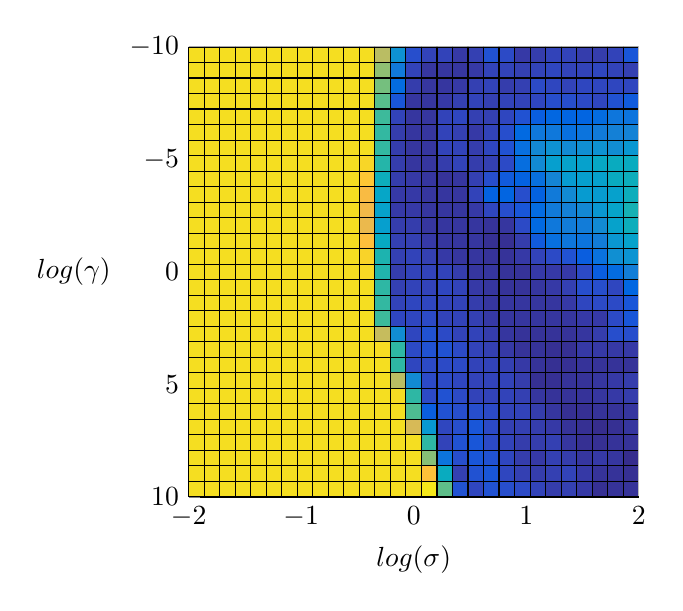
\begin{tikzpicture}

\begin{axis}[%
width=2.25in,
height=2.25in,
at={(0.631944in,0.48125in)},
scale only axis,
xmin=-10,
xmax=10,
xlabel={$log(\gamma)$},
xmajorgrids,
ymin=-2,
ymax=2,
ylabel={$log(\sigma)$},
ymajorgrids,
zmin=0,
zmax=0.4,
zmajorgrids,
view={90}{90},
axis x line*=bottom,
axis y line*=left,
axis z line*=left
]

\addplot3[%
surf,
faceted color=black,
shader=faceted,
colormap={mymap}{[1pt] rgb(0pt)=(0.2081,0.1663,0.5292); rgb(1pt)=(0.211624,0.189781,0.577676); rgb(2pt)=(0.212252,0.213771,0.626971); rgb(3pt)=(0.2081,0.2386,0.677086); rgb(4pt)=(0.195905,0.264457,0.7279); rgb(5pt)=(0.170729,0.291938,0.779248); rgb(6pt)=(0.125271,0.324243,0.830271); rgb(7pt)=(0.0591333,0.359833,0.868333); rgb(8pt)=(0.0116952,0.38751,0.881957); rgb(9pt)=(0.00595714,0.408614,0.882843); rgb(10pt)=(0.0165143,0.4266,0.878633); rgb(11pt)=(0.0328524,0.443043,0.871957); rgb(12pt)=(0.0498143,0.458571,0.864057); rgb(13pt)=(0.0629333,0.47369,0.855438); rgb(14pt)=(0.0722667,0.488667,0.8467); rgb(15pt)=(0.0779429,0.503986,0.838371); rgb(16pt)=(0.0793476,0.520024,0.831181); rgb(17pt)=(0.0749429,0.537543,0.826271); rgb(18pt)=(0.0640571,0.556986,0.823957); rgb(19pt)=(0.0487714,0.577224,0.822829); rgb(20pt)=(0.0343429,0.596581,0.819852); rgb(21pt)=(0.0265,0.6137,0.8135); rgb(22pt)=(0.0238905,0.628662,0.803762); rgb(23pt)=(0.0230905,0.641786,0.791267); rgb(24pt)=(0.0227714,0.653486,0.776757); rgb(25pt)=(0.0266619,0.664195,0.760719); rgb(26pt)=(0.0383714,0.674271,0.743552); rgb(27pt)=(0.0589714,0.683757,0.725386); rgb(28pt)=(0.0843,0.692833,0.706167); rgb(29pt)=(0.113295,0.7015,0.685857); rgb(30pt)=(0.145271,0.709757,0.664629); rgb(31pt)=(0.180133,0.717657,0.642433); rgb(32pt)=(0.217829,0.725043,0.619262); rgb(33pt)=(0.258643,0.731714,0.595429); rgb(34pt)=(0.302171,0.737605,0.571186); rgb(35pt)=(0.348167,0.742433,0.547267); rgb(36pt)=(0.395257,0.7459,0.524443); rgb(37pt)=(0.44201,0.748081,0.503314); rgb(38pt)=(0.487124,0.749062,0.483976); rgb(39pt)=(0.530029,0.749114,0.466114); rgb(40pt)=(0.570857,0.748519,0.44939); rgb(41pt)=(0.609852,0.747314,0.433686); rgb(42pt)=(0.6473,0.7456,0.4188); rgb(43pt)=(0.683419,0.743476,0.404433); rgb(44pt)=(0.71841,0.741133,0.390476); rgb(45pt)=(0.752486,0.7384,0.376814); rgb(46pt)=(0.785843,0.735567,0.363271); rgb(47pt)=(0.818505,0.732733,0.34979); rgb(48pt)=(0.850657,0.7299,0.336029); rgb(49pt)=(0.882433,0.727433,0.3217); rgb(50pt)=(0.913933,0.725786,0.306276); rgb(51pt)=(0.944957,0.726114,0.288643); rgb(52pt)=(0.973895,0.731395,0.266648); rgb(53pt)=(0.993771,0.745457,0.240348); rgb(54pt)=(0.999043,0.765314,0.216414); rgb(55pt)=(0.995533,0.786057,0.196652); rgb(56pt)=(0.988,0.8066,0.179367); rgb(57pt)=(0.978857,0.827143,0.163314); rgb(58pt)=(0.9697,0.848138,0.147452); rgb(59pt)=(0.962586,0.870514,0.1309); rgb(60pt)=(0.958871,0.8949,0.113243); rgb(61pt)=(0.959824,0.921833,0.0948381); rgb(62pt)=(0.9661,0.951443,0.0755333); rgb(63pt)=(0.9763,0.9831,0.0538)},
mesh/rows=30]
table[row sep=crcr,header=false] {%
%
-10	-2	0.33\\
-10	-1.86206896551724	0.33\\
-10	-1.72413793103448	0.33\\
-10	-1.58620689655172	0.33\\
-10	-1.44827586206897	0.33\\
-10	-1.31034482758621	0.33\\
-10	-1.17241379310345	0.33\\
-10	-1.03448275862069	0.33\\
-10	-0.896551724137931	0.33\\
-10	-0.758620689655172	0.33\\
-10	-0.620689655172414	0.33\\
-10	-0.482758620689655	0.33\\
-10	-0.344827586206897	0.33\\
-10	-0.206896551724138	0.21\\
-10	-0.0689655172413792	0.08\\
-10	0.0689655172413794	0.05\\
-10	0.206896551724138	0.07\\
-10	0.344827586206896	0.05\\
-10	0.482758620689655	0.04\\
-10	0.620689655172414	0.07\\
-10	0.758620689655173	0.07\\
-10	0.896551724137931	0.04\\
-10	1.03448275862069	0.04\\
-10	1.17241379310345	0.05\\
-10	1.31034482758621	0.04\\
-10	1.44827586206897	0.06\\
-10	1.58620689655172	0.03\\
-10	1.72413793103448	0.05\\
-10	1.86206896551724	0.06\\
-10	2	0.1\\
-9.31034482758621	-2	0.33\\
-9.31034482758621	-1.86206896551724	0.33\\
-9.31034482758621	-1.72413793103448	0.33\\
-9.31034482758621	-1.58620689655172	0.33\\
-9.31034482758621	-1.44827586206897	0.33\\
-9.31034482758621	-1.31034482758621	0.33\\
-9.31034482758621	-1.17241379310345	0.33\\
-9.31034482758621	-1.03448275862069	0.33\\
-9.31034482758621	-0.896551724137931	0.33\\
-9.31034482758621	-0.758620689655172	0.33\\
-9.31034482758621	-0.620689655172414	0.33\\
-9.31034482758621	-0.482758620689655	0.33\\
-9.31034482758621	-0.344827586206897	0.33\\
-9.31034482758621	-0.206896551724138	0.15\\
-9.31034482758621	-0.0689655172413792	0.06\\
-9.31034482758621	0.0689655172413794	0.04\\
-9.31034482758621	0.206896551724138	0.04\\
-9.31034482758621	0.344827586206896	0.04\\
-9.31034482758621	0.482758620689655	0.04\\
-9.31034482758621	0.620689655172414	0.04\\
-9.31034482758621	0.758620689655173	0.06\\
-9.31034482758621	0.896551724137931	0.05\\
-9.31034482758621	1.03448275862069	0.04\\
-9.31034482758621	1.17241379310345	0.05\\
-9.31034482758621	1.31034482758621	0.06\\
-9.31034482758621	1.44827586206897	0.04\\
-9.31034482758621	1.58620689655172	0.05\\
-9.31034482758621	1.72413793103448	0.05\\
-9.31034482758621	1.86206896551724	0.04\\
-9.31034482758621	2	0.05\\
-8.62068965517241	-2	0.33\\
-8.62068965517241	-1.86206896551724	0.33\\
-8.62068965517241	-1.72413793103448	0.33\\
-8.62068965517241	-1.58620689655172	0.33\\
-8.62068965517241	-1.44827586206897	0.33\\
-8.62068965517241	-1.31034482758621	0.33\\
-8.62068965517241	-1.17241379310345	0.33\\
-8.62068965517241	-1.03448275862069	0.33\\
-8.62068965517241	-0.896551724137931	0.33\\
-8.62068965517241	-0.758620689655172	0.33\\
-8.62068965517241	-0.620689655172414	0.33\\
-8.62068965517241	-0.482758620689655	0.33\\
-8.62068965517241	-0.344827586206897	0.33\\
-8.62068965517241	-0.206896551724138	0.12\\
-8.62068965517241	-0.0689655172413792	0.06\\
-8.62068965517241	0.0689655172413794	0.04\\
-8.62068965517241	0.206896551724138	0.04\\
-8.62068965517241	0.344827586206896	0.04\\
-8.62068965517241	0.482758620689655	0.04\\
-8.62068965517241	0.620689655172414	0.05\\
-8.62068965517241	0.758620689655173	0.05\\
-8.62068965517241	0.896551724137931	0.04\\
-8.62068965517241	1.03448275862069	0.06\\
-8.62068965517241	1.17241379310345	0.05\\
-8.62068965517241	1.31034482758621	0.05\\
-8.62068965517241	1.44827586206897	0.05\\
-8.62068965517241	1.58620689655172	0.06\\
-8.62068965517241	1.72413793103448	0.05\\
-8.62068965517241	1.86206896551724	0.06\\
-8.62068965517241	2	0.04\\
-7.93103448275862	-2	0.33\\
-7.93103448275862	-1.86206896551724	0.33\\
-7.93103448275862	-1.72413793103448	0.33\\
-7.93103448275862	-1.58620689655172	0.33\\
-7.93103448275862	-1.44827586206897	0.33\\
-7.93103448275862	-1.31034482758621	0.33\\
-7.93103448275862	-1.17241379310345	0.33\\
-7.93103448275862	-1.03448275862069	0.33\\
-7.93103448275862	-0.896551724137931	0.33\\
-7.93103448275862	-0.758620689655172	0.33\\
-7.93103448275862	-0.620689655172414	0.33\\
-7.93103448275862	-0.482758620689655	0.33\\
-7.93103448275862	-0.344827586206897	0.33\\
-7.93103448275862	-0.206896551724138	0.1\\
-7.93103448275862	-0.0689655172413792	0.04\\
-7.93103448275862	0.0689655172413794	0.04\\
-7.93103448275862	0.206896551724138	0.04\\
-7.93103448275862	0.344827586206896	0.04\\
-7.93103448275862	0.482758620689655	0.05\\
-7.93103448275862	0.620689655172414	0.05\\
-7.93103448275862	0.758620689655173	0.05\\
-7.93103448275862	0.896551724137931	0.04\\
-7.93103448275862	1.03448275862069	0.05\\
-7.93103448275862	1.17241379310345	0.06\\
-7.93103448275862	1.31034482758621	0.05\\
-7.93103448275862	1.44827586206897	0.05\\
-7.93103448275862	1.58620689655172	0.05\\
-7.93103448275862	1.72413793103448	0.05\\
-7.93103448275862	1.86206896551724	0.05\\
-7.93103448275862	2	0.06\\
-7.24137931034483	-2	0.33\\
-7.24137931034483	-1.86206896551724	0.33\\
-7.24137931034483	-1.72413793103448	0.33\\
-7.24137931034483	-1.58620689655172	0.33\\
-7.24137931034483	-1.44827586206897	0.33\\
-7.24137931034483	-1.31034482758621	0.33\\
-7.24137931034483	-1.17241379310345	0.33\\
-7.24137931034483	-1.03448275862069	0.33\\
-7.24137931034483	-0.896551724137931	0.33\\
-7.24137931034483	-0.758620689655172	0.33\\
-7.24137931034483	-0.620689655172414	0.33\\
-7.24137931034483	-0.482758620689655	0.33\\
-7.24137931034483	-0.344827586206897	0.33\\
-7.24137931034483	-0.206896551724138	0.07\\
-7.24137931034483	-0.0689655172413792	0.04\\
-7.24137931034483	0.0689655172413794	0.04\\
-7.24137931034483	0.206896551724138	0.04\\
-7.24137931034483	0.344827586206896	0.05\\
-7.24137931034483	0.482758620689655	0.05\\
-7.24137931034483	0.620689655172414	0.05\\
-7.24137931034483	0.758620689655173	0.04\\
-7.24137931034483	0.896551724137931	0.07\\
-7.24137931034483	1.03448275862069	0.04\\
-7.24137931034483	1.17241379310345	0.06\\
-7.24137931034483	1.31034482758621	0.06\\
-7.24137931034483	1.44827586206897	0.07\\
-7.24137931034483	1.58620689655172	0.05\\
-7.24137931034483	1.72413793103448	0.06\\
-7.24137931034483	1.86206896551724	0.08\\
-7.24137931034483	2	0.07\\
-6.55172413793103	-2	0.33\\
-6.55172413793103	-1.86206896551724	0.33\\
-6.55172413793103	-1.72413793103448	0.33\\
-6.55172413793103	-1.58620689655172	0.33\\
-6.55172413793103	-1.44827586206897	0.33\\
-6.55172413793103	-1.31034482758621	0.33\\
-6.55172413793103	-1.17241379310345	0.33\\
-6.55172413793103	-1.03448275862069	0.33\\
-6.55172413793103	-0.896551724137931	0.33\\
-6.55172413793103	-0.758620689655172	0.33\\
-6.55172413793103	-0.620689655172414	0.33\\
-6.55172413793103	-0.482758620689655	0.33\\
-6.55172413793103	-0.344827586206897	0.33\\
-6.55172413793103	-0.206896551724138	0.05\\
-6.55172413793103	-0.0689655172413792	0.04\\
-6.55172413793103	0.0689655172413794	0.04\\
-6.55172413793103	0.206896551724138	0.04\\
-6.55172413793103	0.344827586206896	0.07\\
-6.55172413793103	0.482758620689655	0.04\\
-6.55172413793103	0.620689655172414	0.05\\
-6.55172413793103	0.758620689655173	0.05\\
-6.55172413793103	0.896551724137931	0.05\\
-6.55172413793103	1.03448275862069	0.08\\
-6.55172413793103	1.17241379310345	0.09\\
-6.55172413793103	1.31034482758621	0.09\\
-6.55172413793103	1.44827586206897	0.07\\
-6.55172413793103	1.58620689655172	0.1\\
-6.55172413793103	1.72413793103448	0.11\\
-6.55172413793103	1.86206896551724	0.12\\
-6.55172413793103	2	0.09\\
-5.86206896551724	-2	0.33\\
-5.86206896551724	-1.86206896551724	0.33\\
-5.86206896551724	-1.72413793103448	0.33\\
-5.86206896551724	-1.58620689655172	0.33\\
-5.86206896551724	-1.44827586206897	0.33\\
-5.86206896551724	-1.31034482758621	0.33\\
-5.86206896551724	-1.17241379310345	0.33\\
-5.86206896551724	-1.03448275862069	0.33\\
-5.86206896551724	-0.896551724137931	0.33\\
-5.86206896551724	-0.758620689655172	0.33\\
-5.86206896551724	-0.620689655172414	0.33\\
-5.86206896551724	-0.482758620689655	0.33\\
-5.86206896551724	-0.344827586206897	0.33\\
-5.86206896551724	-0.206896551724138	0.05\\
-5.86206896551724	-0.0689655172413792	0.04\\
-5.86206896551724	0.0689655172413794	0.04\\
-5.86206896551724	0.206896551724138	0.04\\
-5.86206896551724	0.344827586206896	0.05\\
-5.86206896551724	0.482758620689655	0.03\\
-5.86206896551724	0.620689655172414	0.05\\
-5.86206896551724	0.758620689655173	0.05\\
-5.86206896551724	0.896551724137931	0.08\\
-5.86206896551724	1.03448275862069	0.1\\
-5.86206896551724	1.17241379310345	0.11\\
-5.86206896551724	1.31034482758621	0.09\\
-5.86206896551724	1.44827586206897	0.09\\
-5.86206896551724	1.58620689655172	0.1\\
-5.86206896551724	1.72413793103448	0.08\\
-5.86206896551724	1.86206896551724	0.11\\
-5.86206896551724	2	0.11\\
-5.17241379310345	-2	0.33\\
-5.17241379310345	-1.86206896551724	0.33\\
-5.17241379310345	-1.72413793103448	0.33\\
-5.17241379310345	-1.58620689655172	0.33\\
-5.17241379310345	-1.44827586206897	0.33\\
-5.17241379310345	-1.31034482758621	0.33\\
-5.17241379310345	-1.17241379310345	0.33\\
-5.17241379310345	-1.03448275862069	0.33\\
-5.17241379310345	-0.896551724137931	0.33\\
-5.17241379310345	-0.758620689655172	0.33\\
-5.17241379310345	-0.620689655172414	0.33\\
-5.17241379310345	-0.482758620689655	0.33\\
-5.17241379310345	-0.344827586206897	0.33\\
-5.17241379310345	-0.206896551724138	0.05\\
-5.17241379310345	-0.0689655172413792	0.04\\
-5.17241379310345	0.0689655172413794	0.04\\
-5.17241379310345	0.206896551724138	0.04\\
-5.17241379310345	0.344827586206896	0.07\\
-5.17241379310345	0.482758620689655	0.05\\
-5.17241379310345	0.620689655172414	0.05\\
-5.17241379310345	0.758620689655173	0.06\\
-5.17241379310345	0.896551724137931	0.05\\
-5.17241379310345	1.03448275862069	0.11\\
-5.17241379310345	1.17241379310345	0.14\\
-5.17241379310345	1.31034482758621	0.16\\
-5.17241379310345	1.44827586206897	0.13\\
-5.17241379310345	1.58620689655172	0.17\\
-5.17241379310345	1.72413793103448	0.15\\
-5.17241379310345	1.86206896551724	0.14\\
-5.17241379310345	2	0.16\\
-4.48275862068965	-2	0.33\\
-4.48275862068965	-1.86206896551724	0.33\\
-4.48275862068965	-1.72413793103448	0.33\\
-4.48275862068965	-1.58620689655172	0.33\\
-4.48275862068965	-1.44827586206897	0.33\\
-4.48275862068965	-1.31034482758621	0.33\\
-4.48275862068965	-1.17241379310345	0.33\\
-4.48275862068965	-1.03448275862069	0.33\\
-4.48275862068965	-0.896551724137931	0.33\\
-4.48275862068965	-0.758620689655172	0.33\\
-4.48275862068965	-0.620689655172414	0.33\\
-4.48275862068965	-0.482758620689655	0.33\\
-4.48275862068965	-0.344827586206897	0.3\\
-4.48275862068965	-0.206896551724138	0.05\\
-4.48275862068965	-0.0689655172413792	0.04\\
-4.48275862068965	0.0689655172413794	0.04\\
-4.48275862068965	0.206896551724138	0.04\\
-4.48275862068965	0.344827586206896	0.03\\
-4.48275862068965	0.482758620689655	0.05\\
-4.48275862068965	0.620689655172414	0.03\\
-4.48275862068965	0.758620689655173	0.05\\
-4.48275862068965	0.896551724137931	0.06\\
-4.48275862068965	1.03448275862069	0.11\\
-4.48275862068965	1.17241379310345	0.11\\
-4.48275862068965	1.31034482758621	0.15\\
-4.48275862068965	1.44827586206897	0.14\\
-4.48275862068965	1.58620689655172	0.13\\
-4.48275862068965	1.72413793103448	0.17\\
-4.48275862068965	1.86206896551724	0.18\\
-4.48275862068965	2	0.16\\
-3.79310344827586	-2	0.33\\
-3.79310344827586	-1.86206896551724	0.33\\
-3.79310344827586	-1.72413793103448	0.33\\
-3.79310344827586	-1.58620689655172	0.33\\
-3.79310344827586	-1.44827586206897	0.33\\
-3.79310344827586	-1.31034482758621	0.33\\
-3.79310344827586	-1.17241379310345	0.33\\
-3.79310344827586	-1.03448275862069	0.33\\
-3.79310344827586	-0.896551724137931	0.33\\
-3.79310344827586	-0.758620689655172	0.33\\
-3.79310344827586	-0.620689655172414	0.33\\
-3.79310344827586	-0.482758620689655	0.33\\
-3.79310344827586	-0.344827586206897	0.27\\
-3.79310344827586	-0.206896551724138	0.04\\
-3.79310344827586	-0.0689655172413792	0.05\\
-3.79310344827586	0.0689655172413794	0.04\\
-3.79310344827586	0.206896551724138	0.04\\
-3.79310344827586	0.344827586206896	0.04\\
-3.79310344827586	0.482758620689655	0.04\\
-3.79310344827586	0.620689655172414	0.07\\
-3.79310344827586	0.758620689655173	0.08\\
-3.79310344827586	0.896551724137931	0.07\\
-3.79310344827586	1.03448275862069	0.04\\
-3.79310344827586	1.17241379310345	0.08\\
-3.79310344827586	1.31034482758621	0.1\\
-3.79310344827586	1.44827586206897	0.15\\
-3.79310344827586	1.58620689655172	0.14\\
-3.79310344827586	1.72413793103448	0.13\\
-3.79310344827586	1.86206896551724	0.16\\
-3.79310344827586	2	0.16\\
-3.10344827586207	-2	0.33\\
-3.10344827586207	-1.86206896551724	0.33\\
-3.10344827586207	-1.72413793103448	0.33\\
-3.10344827586207	-1.58620689655172	0.33\\
-3.10344827586207	-1.44827586206897	0.33\\
-3.10344827586207	-1.31034482758621	0.33\\
-3.10344827586207	-1.17241379310345	0.33\\
-3.10344827586207	-1.03448275862069	0.33\\
-3.10344827586207	-0.896551724137931	0.33\\
-3.10344827586207	-0.758620689655172	0.33\\
-3.10344827586207	-0.620689655172414	0.33\\
-3.10344827586207	-0.482758620689655	0.33\\
-3.10344827586207	-0.344827586206897	0.25\\
-3.10344827586207	-0.206896551724138	0.04\\
-3.10344827586207	-0.0689655172413792	0.04\\
-3.10344827586207	0.0689655172413794	0.04\\
-3.10344827586207	0.206896551724138	0.04\\
-3.10344827586207	0.344827586206896	0.04\\
-3.10344827586207	0.482758620689655	0.04\\
-3.10344827586207	0.620689655172414	0.05\\
-3.10344827586207	0.758620689655173	0.08\\
-3.10344827586207	0.896551724137931	0.06\\
-3.10344827586207	1.03448275862069	0.06\\
-3.10344827586207	1.17241379310345	0.1\\
-3.10344827586207	1.31034482758621	0.11\\
-3.10344827586207	1.44827586206897	0.11\\
-3.10344827586207	1.58620689655172	0.14\\
-3.10344827586207	1.72413793103448	0.13\\
-3.10344827586207	1.86206896551724	0.15\\
-3.10344827586207	2	0.19\\
-2.41379310344828	-2	0.33\\
-2.41379310344828	-1.86206896551724	0.33\\
-2.41379310344828	-1.72413793103448	0.33\\
-2.41379310344828	-1.58620689655172	0.33\\
-2.41379310344828	-1.44827586206897	0.33\\
-2.41379310344828	-1.31034482758621	0.33\\
-2.41379310344828	-1.17241379310345	0.33\\
-2.41379310344828	-1.03448275862069	0.33\\
-2.41379310344828	-0.896551724137931	0.33\\
-2.41379310344828	-0.758620689655172	0.33\\
-2.41379310344828	-0.620689655172414	0.33\\
-2.41379310344828	-0.482758620689655	0.33\\
-2.41379310344828	-0.344827586206897	0.25\\
-2.41379310344828	-0.206896551724138	0.04\\
-2.41379310344828	-0.0689655172413792	0.05\\
-2.41379310344828	0.0689655172413794	0.04\\
-2.41379310344828	0.206896551724138	0.04\\
-2.41379310344828	0.344827586206896	0.04\\
-2.41379310344828	0.482758620689655	0.04\\
-2.41379310344828	0.620689655172414	0.04\\
-2.41379310344828	0.758620689655173	0.04\\
-2.41379310344828	0.896551724137931	0.05\\
-2.41379310344828	1.03448275862069	0.08\\
-2.41379310344828	1.17241379310345	0.08\\
-2.41379310344828	1.31034482758621	0.1\\
-2.41379310344828	1.44827586206897	0.1\\
-2.41379310344828	1.58620689655172	0.11\\
-2.41379310344828	1.72413793103448	0.14\\
-2.41379310344828	1.86206896551724	0.17\\
-2.41379310344828	2	0.18\\
-1.72413793103448	-2	0.33\\
-1.72413793103448	-1.86206896551724	0.33\\
-1.72413793103448	-1.72413793103448	0.33\\
-1.72413793103448	-1.58620689655172	0.33\\
-1.72413793103448	-1.44827586206897	0.33\\
-1.72413793103448	-1.31034482758621	0.33\\
-1.72413793103448	-1.17241379310345	0.33\\
-1.72413793103448	-1.03448275862069	0.33\\
-1.72413793103448	-0.896551724137931	0.33\\
-1.72413793103448	-0.758620689655172	0.33\\
-1.72413793103448	-0.620689655172414	0.33\\
-1.72413793103448	-0.482758620689655	0.33\\
-1.72413793103448	-0.344827586206897	0.23\\
-1.72413793103448	-0.206896551724138	0.04\\
-1.72413793103448	-0.0689655172413792	0.05\\
-1.72413793103448	0.0689655172413794	0.04\\
-1.72413793103448	0.206896551724138	0.04\\
-1.72413793103448	0.344827586206896	0.04\\
-1.72413793103448	0.482758620689655	0.04\\
-1.72413793103448	0.620689655172414	0.04\\
-1.72413793103448	0.758620689655173	0.03\\
-1.72413793103448	0.896551724137931	0.04\\
-1.72413793103448	1.03448275862069	0.05\\
-1.72413793103448	1.17241379310345	0.1\\
-1.72413793103448	1.31034482758621	0.1\\
-1.72413793103448	1.44827586206897	0.1\\
-1.72413793103448	1.58620689655172	0.09\\
-1.72413793103448	1.72413793103448	0.13\\
-1.72413793103448	1.86206896551724	0.14\\
-1.72413793103448	2	0.17\\
-1.03448275862069	-2	0.33\\
-1.03448275862069	-1.86206896551724	0.33\\
-1.03448275862069	-1.72413793103448	0.33\\
-1.03448275862069	-1.58620689655172	0.33\\
-1.03448275862069	-1.44827586206897	0.33\\
-1.03448275862069	-1.31034482758621	0.33\\
-1.03448275862069	-1.17241379310345	0.33\\
-1.03448275862069	-1.03448275862069	0.33\\
-1.03448275862069	-0.896551724137931	0.33\\
-1.03448275862069	-0.758620689655172	0.33\\
-1.03448275862069	-0.620689655172414	0.33\\
-1.03448275862069	-0.482758620689655	0.33\\
-1.03448275862069	-0.344827586206897	0.31\\
-1.03448275862069	-0.206896551724138	0.05\\
-1.03448275862069	-0.0689655172413792	0.05\\
-1.03448275862069	0.0689655172413794	0.05\\
-1.03448275862069	0.206896551724138	0.04\\
-1.03448275862069	0.344827586206896	0.04\\
-1.03448275862069	0.482758620689655	0.04\\
-1.03448275862069	0.620689655172414	0.04\\
-1.03448275862069	0.758620689655173	0.03\\
-1.03448275862069	0.896551724137931	0.04\\
-1.03448275862069	1.03448275862069	0.05\\
-1.03448275862069	1.17241379310345	0.06\\
-1.03448275862069	1.31034482758621	0.08\\
-1.03448275862069	1.44827586206897	0.09\\
-1.03448275862069	1.58620689655172	0.08\\
-1.03448275862069	1.72413793103448	0.1\\
-1.03448275862069	1.86206896551724	0.15\\
-1.03448275862069	2	0.12\\
-0.344827586206897	-2	0.33\\
-0.344827586206897	-1.86206896551724	0.33\\
-0.344827586206897	-1.72413793103448	0.33\\
-0.344827586206897	-1.58620689655172	0.33\\
-0.344827586206897	-1.44827586206897	0.33\\
-0.344827586206897	-1.31034482758621	0.33\\
-0.344827586206897	-1.17241379310345	0.33\\
-0.344827586206897	-1.03448275862069	0.33\\
-0.344827586206897	-0.896551724137931	0.33\\
-0.344827586206897	-0.758620689655172	0.33\\
-0.344827586206897	-0.620689655172414	0.33\\
-0.344827586206897	-0.482758620689655	0.33\\
-0.344827586206897	-0.344827586206897	0.31\\
-0.344827586206897	-0.206896551724138	0.04\\
-0.344827586206897	-0.0689655172413792	0.05\\
-0.344827586206897	0.0689655172413794	0.05\\
-0.344827586206897	0.206896551724138	0.05\\
-0.344827586206897	0.344827586206896	0.04\\
-0.344827586206897	0.482758620689655	0.04\\
-0.344827586206897	0.620689655172414	0.04\\
-0.344827586206897	0.758620689655173	0.04\\
-0.344827586206897	0.896551724137931	0.04\\
-0.344827586206897	1.03448275862069	0.04\\
-0.344827586206897	1.17241379310345	0.05\\
-0.344827586206897	1.31034482758621	0.03\\
-0.344827586206897	1.44827586206897	0.04\\
-0.344827586206897	1.58620689655172	0.06\\
-0.344827586206897	1.72413793103448	0.11\\
-0.344827586206897	1.86206896551724	0.13\\
-0.344827586206897	2	0.11\\
0.344827586206897	-2	0.33\\
0.344827586206897	-1.86206896551724	0.33\\
0.344827586206897	-1.72413793103448	0.33\\
0.344827586206897	-1.58620689655172	0.33\\
0.344827586206897	-1.44827586206897	0.33\\
0.344827586206897	-1.31034482758621	0.33\\
0.344827586206897	-1.17241379310345	0.33\\
0.344827586206897	-1.03448275862069	0.33\\
0.344827586206897	-0.896551724137931	0.33\\
0.344827586206897	-0.758620689655172	0.33\\
0.344827586206897	-0.620689655172414	0.33\\
0.344827586206897	-0.482758620689655	0.33\\
0.344827586206897	-0.344827586206897	0.33\\
0.344827586206897	-0.206896551724138	0.04\\
0.344827586206897	-0.0689655172413792	0.05\\
0.344827586206897	0.0689655172413794	0.05\\
0.344827586206897	0.206896551724138	0.05\\
0.344827586206897	0.344827586206896	0.06\\
0.344827586206897	0.482758620689655	0.04\\
0.344827586206897	0.620689655172414	0.04\\
0.344827586206897	0.758620689655173	0.04\\
0.344827586206897	0.896551724137931	0.03\\
0.344827586206897	1.03448275862069	0.04\\
0.344827586206897	1.17241379310345	0.04\\
0.344827586206897	1.31034482758621	0.05\\
0.344827586206897	1.44827586206897	0.05\\
0.344827586206897	1.58620689655172	0.07\\
0.344827586206897	1.72413793103448	0.03\\
0.344827586206897	1.86206896551724	0.05\\
0.344827586206897	2	0.12\\
1.03448275862069	-2	0.33\\
1.03448275862069	-1.86206896551724	0.33\\
1.03448275862069	-1.72413793103448	0.33\\
1.03448275862069	-1.58620689655172	0.33\\
1.03448275862069	-1.44827586206897	0.33\\
1.03448275862069	-1.31034482758621	0.33\\
1.03448275862069	-1.17241379310345	0.33\\
1.03448275862069	-1.03448275862069	0.33\\
1.03448275862069	-0.896551724137931	0.33\\
1.03448275862069	-0.758620689655172	0.33\\
1.03448275862069	-0.620689655172414	0.33\\
1.03448275862069	-0.482758620689655	0.33\\
1.03448275862069	-0.344827586206897	0.33\\
1.03448275862069	-0.206896551724138	0.05\\
1.03448275862069	-0.0689655172413792	0.05\\
1.03448275862069	0.0689655172413794	0.05\\
1.03448275862069	0.206896551724138	0.05\\
1.03448275862069	0.344827586206896	0.05\\
1.03448275862069	0.482758620689655	0.05\\
1.03448275862069	0.620689655172414	0.04\\
1.03448275862069	0.758620689655173	0.04\\
1.03448275862069	0.896551724137931	0.04\\
1.03448275862069	1.03448275862069	0.04\\
1.03448275862069	1.17241379310345	0.04\\
1.03448275862069	1.31034482758621	0.04\\
1.03448275862069	1.44827586206897	0.05\\
1.03448275862069	1.58620689655172	0.06\\
1.03448275862069	1.72413793103448	0.07\\
1.03448275862069	1.86206896551724	0.06\\
1.03448275862069	2	0.07\\
1.72413793103448	-2	0.33\\
1.72413793103448	-1.86206896551724	0.33\\
1.72413793103448	-1.72413793103448	0.33\\
1.72413793103448	-1.58620689655172	0.33\\
1.72413793103448	-1.44827586206897	0.33\\
1.72413793103448	-1.31034482758621	0.33\\
1.72413793103448	-1.17241379310345	0.33\\
1.72413793103448	-1.03448275862069	0.33\\
1.72413793103448	-0.896551724137931	0.33\\
1.72413793103448	-0.758620689655172	0.33\\
1.72413793103448	-0.620689655172414	0.33\\
1.72413793103448	-0.482758620689655	0.33\\
1.72413793103448	-0.344827586206897	0.33\\
1.72413793103448	-0.206896551724138	0.05\\
1.72413793103448	-0.0689655172413792	0.05\\
1.72413793103448	0.0689655172413794	0.06\\
1.72413793103448	0.206896551724138	0.05\\
1.72413793103448	0.344827586206896	0.05\\
1.72413793103448	0.482758620689655	0.05\\
1.72413793103448	0.620689655172414	0.04\\
1.72413793103448	0.758620689655173	0.04\\
1.72413793103448	0.896551724137931	0.04\\
1.72413793103448	1.03448275862069	0.04\\
1.72413793103448	1.17241379310345	0.04\\
1.72413793103448	1.31034482758621	0.04\\
1.72413793103448	1.44827586206897	0.04\\
1.72413793103448	1.58620689655172	0.06\\
1.72413793103448	1.72413793103448	0.03\\
1.72413793103448	1.86206896551724	0.06\\
1.72413793103448	2	0.06\\
2.41379310344828	-2	0.33\\
2.41379310344828	-1.86206896551724	0.33\\
2.41379310344828	-1.72413793103448	0.33\\
2.41379310344828	-1.58620689655172	0.33\\
2.41379310344828	-1.44827586206897	0.33\\
2.41379310344828	-1.31034482758621	0.33\\
2.41379310344828	-1.17241379310345	0.33\\
2.41379310344828	-1.03448275862069	0.33\\
2.41379310344828	-0.896551724137931	0.33\\
2.41379310344828	-0.758620689655172	0.33\\
2.41379310344828	-0.620689655172414	0.33\\
2.41379310344828	-0.482758620689655	0.33\\
2.41379310344828	-0.344827586206897	0.33\\
2.41379310344828	-0.206896551724138	0.07\\
2.41379310344828	-0.0689655172413792	0.04\\
2.41379310344828	0.0689655172413794	0.06\\
2.41379310344828	0.206896551724138	0.05\\
2.41379310344828	0.344827586206896	0.05\\
2.41379310344828	0.482758620689655	0.05\\
2.41379310344828	0.620689655172414	0.05\\
2.41379310344828	0.758620689655173	0.04\\
2.41379310344828	0.896551724137931	0.04\\
2.41379310344828	1.03448275862069	0.04\\
2.41379310344828	1.17241379310345	0.04\\
2.41379310344828	1.31034482758621	0.04\\
2.41379310344828	1.44827586206897	0.04\\
2.41379310344828	1.58620689655172	0.03\\
2.41379310344828	1.72413793103448	0.05\\
2.41379310344828	1.86206896551724	0.08\\
2.41379310344828	2	0.05\\
3.10344827586207	-2	0.33\\
3.10344827586207	-1.86206896551724	0.33\\
3.10344827586207	-1.72413793103448	0.33\\
3.10344827586207	-1.58620689655172	0.33\\
3.10344827586207	-1.44827586206897	0.33\\
3.10344827586207	-1.31034482758621	0.33\\
3.10344827586207	-1.17241379310345	0.33\\
3.10344827586207	-1.03448275862069	0.33\\
3.10344827586207	-0.896551724137931	0.33\\
3.10344827586207	-0.758620689655172	0.33\\
3.10344827586207	-0.620689655172414	0.33\\
3.10344827586207	-0.482758620689655	0.33\\
3.10344827586207	-0.344827586206897	0.33\\
3.10344827586207	-0.206896551724138	0.32\\
3.10344827586207	-0.0689655172413792	0.05\\
3.10344827586207	0.0689655172413794	0.06\\
3.10344827586207	0.206896551724138	0.07\\
3.10344827586207	0.344827586206896	0.05\\
3.10344827586207	0.482758620689655	0.05\\
3.10344827586207	0.620689655172414	0.05\\
3.10344827586207	0.758620689655173	0.04\\
3.10344827586207	0.896551724137931	0.04\\
3.10344827586207	1.03448275862069	0.03\\
3.10344827586207	1.17241379310345	0.04\\
3.10344827586207	1.31034482758621	0.03\\
3.10344827586207	1.44827586206897	0.04\\
3.10344827586207	1.58620689655172	0.05\\
3.10344827586207	1.72413793103448	0.05\\
3.10344827586207	1.86206896551724	0.05\\
3.10344827586207	2	0.05\\
3.79310344827586	-2	0.33\\
3.79310344827586	-1.86206896551724	0.33\\
3.79310344827586	-1.72413793103448	0.33\\
3.79310344827586	-1.58620689655172	0.33\\
3.79310344827586	-1.44827586206897	0.33\\
3.79310344827586	-1.31034482758621	0.33\\
3.79310344827586	-1.17241379310345	0.33\\
3.79310344827586	-1.03448275862069	0.33\\
3.79310344827586	-0.896551724137931	0.33\\
3.79310344827586	-0.758620689655172	0.33\\
3.79310344827586	-0.620689655172414	0.33\\
3.79310344827586	-0.482758620689655	0.33\\
3.79310344827586	-0.344827586206897	0.33\\
3.79310344827586	-0.206896551724138	0.33\\
3.79310344827586	-0.0689655172413792	0.05\\
3.79310344827586	0.0689655172413794	0.06\\
3.79310344827586	0.206896551724138	0.05\\
3.79310344827586	0.344827586206896	0.07\\
3.79310344827586	0.482758620689655	0.05\\
3.79310344827586	0.620689655172414	0.05\\
3.79310344827586	0.758620689655173	0.05\\
3.79310344827586	0.896551724137931	0.04\\
3.79310344827586	1.03448275862069	0.04\\
3.79310344827586	1.17241379310345	0.04\\
3.79310344827586	1.31034482758621	0.03\\
3.79310344827586	1.44827586206897	0.04\\
3.79310344827586	1.58620689655172	0.04\\
3.79310344827586	1.72413793103448	0.03\\
3.79310344827586	1.86206896551724	0.04\\
3.79310344827586	2	0.03\\
4.48275862068965	-2	0.33\\
4.48275862068965	-1.86206896551724	0.33\\
4.48275862068965	-1.72413793103448	0.33\\
4.48275862068965	-1.58620689655172	0.33\\
4.48275862068965	-1.44827586206897	0.33\\
4.48275862068965	-1.31034482758621	0.33\\
4.48275862068965	-1.17241379310345	0.33\\
4.48275862068965	-1.03448275862069	0.33\\
4.48275862068965	-0.896551724137931	0.33\\
4.48275862068965	-0.758620689655172	0.33\\
4.48275862068965	-0.620689655172414	0.33\\
4.48275862068965	-0.482758620689655	0.33\\
4.48275862068965	-0.344827586206897	0.33\\
4.48275862068965	-0.206896551724138	0.33\\
4.48275862068965	-0.0689655172413792	0.04\\
4.48275862068965	0.0689655172413794	0.06\\
4.48275862068965	0.206896551724138	0.05\\
4.48275862068965	0.344827586206896	0.05\\
4.48275862068965	0.482758620689655	0.05\\
4.48275862068965	0.620689655172414	0.05\\
4.48275862068965	0.758620689655173	0.05\\
4.48275862068965	0.896551724137931	0.05\\
4.48275862068965	1.03448275862069	0.04\\
4.48275862068965	1.17241379310345	0.03\\
4.48275862068965	1.31034482758621	0.04\\
4.48275862068965	1.44827586206897	0.03\\
4.48275862068965	1.58620689655172	0.04\\
4.48275862068965	1.72413793103448	0.04\\
4.48275862068965	1.86206896551724	0.04\\
4.48275862068965	2	0.04\\
5.17241379310345	-2	0.33\\
5.17241379310345	-1.86206896551724	0.33\\
5.17241379310345	-1.72413793103448	0.33\\
5.17241379310345	-1.58620689655172	0.33\\
5.17241379310345	-1.44827586206897	0.33\\
5.17241379310345	-1.31034482758621	0.33\\
5.17241379310345	-1.17241379310345	0.33\\
5.17241379310345	-1.03448275862069	0.33\\
5.17241379310345	-0.896551724137931	0.33\\
5.17241379310345	-0.758620689655172	0.33\\
5.17241379310345	-0.620689655172414	0.33\\
5.17241379310345	-0.482758620689655	0.33\\
5.17241379310345	-0.344827586206897	0.33\\
5.17241379310345	-0.206896551724138	0.33\\
5.17241379310345	-0.0689655172413792	0.32\\
5.17241379310345	0.0689655172413794	0.05\\
5.17241379310345	0.206896551724138	0.06\\
5.17241379310345	0.344827586206896	0.06\\
5.17241379310345	0.482758620689655	0.05\\
5.17241379310345	0.620689655172414	0.05\\
5.17241379310345	0.758620689655173	0.05\\
5.17241379310345	0.896551724137931	0.05\\
5.17241379310345	1.03448275862069	0.04\\
5.17241379310345	1.17241379310345	0.03\\
5.17241379310345	1.31034482758621	0.04\\
5.17241379310345	1.44827586206897	0.04\\
5.17241379310345	1.58620689655172	0.04\\
5.17241379310345	1.72413793103448	0.04\\
5.17241379310345	1.86206896551724	0.05\\
5.17241379310345	2	0.05\\
5.86206896551724	-2	0.33\\
5.86206896551724	-1.86206896551724	0.33\\
5.86206896551724	-1.72413793103448	0.33\\
5.86206896551724	-1.58620689655172	0.33\\
5.86206896551724	-1.44827586206897	0.33\\
5.86206896551724	-1.31034482758621	0.33\\
5.86206896551724	-1.17241379310345	0.33\\
5.86206896551724	-1.03448275862069	0.33\\
5.86206896551724	-0.896551724137931	0.33\\
5.86206896551724	-0.758620689655172	0.33\\
5.86206896551724	-0.620689655172414	0.33\\
5.86206896551724	-0.482758620689655	0.33\\
5.86206896551724	-0.344827586206897	0.33\\
5.86206896551724	-0.206896551724138	0.33\\
5.86206896551724	-0.0689655172413792	0.33\\
5.86206896551724	0.0689655172413794	0.05\\
5.86206896551724	0.206896551724138	0.06\\
5.86206896551724	0.344827586206896	0.06\\
5.86206896551724	0.482758620689655	0.05\\
5.86206896551724	0.620689655172414	0.05\\
5.86206896551724	0.758620689655173	0.05\\
5.86206896551724	0.896551724137931	0.05\\
5.86206896551724	1.03448275862069	0.05\\
5.86206896551724	1.17241379310345	0.04\\
5.86206896551724	1.31034482758621	0.04\\
5.86206896551724	1.44827586206897	0.03\\
5.86206896551724	1.58620689655172	0.04\\
5.86206896551724	1.72413793103448	0.04\\
5.86206896551724	1.86206896551724	0.04\\
5.86206896551724	2	0.04\\
6.55172413793104	-2	0.33\\
6.55172413793104	-1.86206896551724	0.33\\
6.55172413793104	-1.72413793103448	0.33\\
6.55172413793104	-1.58620689655172	0.33\\
6.55172413793104	-1.44827586206897	0.33\\
6.55172413793104	-1.31034482758621	0.33\\
6.55172413793104	-1.17241379310345	0.33\\
6.55172413793104	-1.03448275862069	0.33\\
6.55172413793104	-0.896551724137931	0.33\\
6.55172413793104	-0.758620689655172	0.33\\
6.55172413793104	-0.620689655172414	0.33\\
6.55172413793104	-0.482758620689655	0.33\\
6.55172413793104	-0.344827586206897	0.33\\
6.55172413793104	-0.206896551724138	0.33\\
6.55172413793104	-0.0689655172413792	0.33\\
6.55172413793104	0.0689655172413794	0.1\\
6.55172413793104	0.206896551724138	0.06\\
6.55172413793104	0.344827586206896	0.06\\
6.55172413793104	0.482758620689655	0.06\\
6.55172413793104	0.620689655172414	0.07\\
6.55172413793104	0.758620689655173	0.05\\
6.55172413793104	0.896551724137931	0.05\\
6.55172413793104	1.03448275862069	0.05\\
6.55172413793104	1.17241379310345	0.04\\
6.55172413793104	1.31034482758621	0.04\\
6.55172413793104	1.44827586206897	0.03\\
6.55172413793104	1.58620689655172	0.04\\
6.55172413793104	1.72413793103448	0.03\\
6.55172413793104	1.86206896551724	0.04\\
6.55172413793104	2	0.04\\
7.24137931034483	-2	0.33\\
7.24137931034483	-1.86206896551724	0.33\\
7.24137931034483	-1.72413793103448	0.33\\
7.24137931034483	-1.58620689655172	0.33\\
7.24137931034483	-1.44827586206897	0.33\\
7.24137931034483	-1.31034482758621	0.33\\
7.24137931034483	-1.17241379310345	0.33\\
7.24137931034483	-1.03448275862069	0.33\\
7.24137931034483	-0.896551724137931	0.33\\
7.24137931034483	-0.758620689655172	0.33\\
7.24137931034483	-0.620689655172414	0.33\\
7.24137931034483	-0.482758620689655	0.33\\
7.24137931034483	-0.344827586206897	0.33\\
7.24137931034483	-0.206896551724138	0.33\\
7.24137931034483	-0.0689655172413792	0.33\\
7.24137931034483	0.0689655172413794	0.33\\
7.24137931034483	0.206896551724138	0.04\\
7.24137931034483	0.344827586206896	0.05\\
7.24137931034483	0.482758620689655	0.06\\
7.24137931034483	0.620689655172414	0.06\\
7.24137931034483	0.758620689655173	0.04\\
7.24137931034483	0.896551724137931	0.05\\
7.24137931034483	1.03448275862069	0.04\\
7.24137931034483	1.17241379310345	0.05\\
7.24137931034483	1.31034482758621	0.04\\
7.24137931034483	1.44827586206897	0.04\\
7.24137931034483	1.58620689655172	0.03\\
7.24137931034483	1.72413793103448	0.03\\
7.24137931034483	1.86206896551724	0.04\\
7.24137931034483	2	0.04\\
7.93103448275862	-2	0.33\\
7.93103448275862	-1.86206896551724	0.33\\
7.93103448275862	-1.72413793103448	0.33\\
7.93103448275862	-1.58620689655172	0.33\\
7.93103448275862	-1.44827586206897	0.33\\
7.93103448275862	-1.31034482758621	0.33\\
7.93103448275862	-1.17241379310345	0.33\\
7.93103448275862	-1.03448275862069	0.33\\
7.93103448275862	-0.896551724137931	0.33\\
7.93103448275862	-0.758620689655172	0.33\\
7.93103448275862	-0.620689655172414	0.33\\
7.93103448275862	-0.482758620689655	0.33\\
7.93103448275862	-0.344827586206897	0.33\\
7.93103448275862	-0.206896551724138	0.33\\
7.93103448275862	-0.0689655172413792	0.33\\
7.93103448275862	0.0689655172413794	0.33\\
7.93103448275862	0.206896551724138	0.05\\
7.93103448275862	0.344827586206896	0.06\\
7.93103448275862	0.482758620689655	0.07\\
7.93103448275862	0.620689655172414	0.06\\
7.93103448275862	0.758620689655173	0.06\\
7.93103448275862	0.896551724137931	0.05\\
7.93103448275862	1.03448275862069	0.04\\
7.93103448275862	1.17241379310345	0.05\\
7.93103448275862	1.31034482758621	0.05\\
7.93103448275862	1.44827586206897	0.03\\
7.93103448275862	1.58620689655172	0.04\\
7.93103448275862	1.72413793103448	0.04\\
7.93103448275862	1.86206896551724	0.04\\
7.93103448275862	2	0.03\\
8.62068965517241	-2	0.33\\
8.62068965517241	-1.86206896551724	0.33\\
8.62068965517241	-1.72413793103448	0.33\\
8.62068965517241	-1.58620689655172	0.33\\
8.62068965517241	-1.44827586206897	0.33\\
8.62068965517241	-1.31034482758621	0.33\\
8.62068965517241	-1.17241379310345	0.33\\
8.62068965517241	-1.03448275862069	0.33\\
8.62068965517241	-0.896551724137931	0.33\\
8.62068965517241	-0.758620689655172	0.33\\
8.62068965517241	-0.620689655172414	0.33\\
8.62068965517241	-0.482758620689655	0.33\\
8.62068965517241	-0.344827586206897	0.33\\
8.62068965517241	-0.206896551724138	0.33\\
8.62068965517241	-0.0689655172413792	0.33\\
8.62068965517241	0.0689655172413794	0.33\\
8.62068965517241	0.206896551724138	0.2\\
8.62068965517241	0.344827586206896	0.05\\
8.62068965517241	0.482758620689655	0.05\\
8.62068965517241	0.620689655172414	0.07\\
8.62068965517241	0.758620689655173	0.05\\
8.62068965517241	0.896551724137931	0.05\\
8.62068965517241	1.03448275862069	0.04\\
8.62068965517241	1.17241379310345	0.04\\
8.62068965517241	1.31034482758621	0.05\\
8.62068965517241	1.44827586206897	0.05\\
8.62068965517241	1.58620689655172	0.04\\
8.62068965517241	1.72413793103448	0.05\\
8.62068965517241	1.86206896551724	0.03\\
8.62068965517241	2	0.03\\
9.31034482758621	-2	0.33\\
9.31034482758621	-1.86206896551724	0.33\\
9.31034482758621	-1.72413793103448	0.33\\
9.31034482758621	-1.58620689655172	0.33\\
9.31034482758621	-1.44827586206897	0.33\\
9.31034482758621	-1.31034482758621	0.33\\
9.31034482758621	-1.17241379310345	0.33\\
9.31034482758621	-1.03448275862069	0.33\\
9.31034482758621	-0.896551724137931	0.33\\
9.31034482758621	-0.758620689655172	0.33\\
9.31034482758621	-0.620689655172414	0.33\\
9.31034482758621	-0.482758620689655	0.33\\
9.31034482758621	-0.344827586206897	0.33\\
9.31034482758621	-0.206896551724138	0.33\\
9.31034482758621	-0.0689655172413792	0.33\\
9.31034482758621	0.0689655172413794	0.33\\
9.31034482758621	0.206896551724138	0.35\\
9.31034482758621	0.344827586206896	0.04\\
9.31034482758621	0.482758620689655	0.05\\
9.31034482758621	0.620689655172414	0.07\\
9.31034482758621	0.758620689655173	0.06\\
9.31034482758621	0.896551724137931	0.05\\
9.31034482758621	1.03448275862069	0.05\\
9.31034482758621	1.17241379310345	0.05\\
9.31034482758621	1.31034482758621	0.05\\
9.31034482758621	1.44827586206897	0.05\\
9.31034482758621	1.58620689655172	0.03\\
9.31034482758621	1.72413793103448	0.03\\
9.31034482758621	1.86206896551724	0.04\\
9.31034482758621	2	0.04\\
10	-2	0.33\\
10	-1.86206896551724	0.33\\
10	-1.72413793103448	0.33\\
10	-1.58620689655172	0.33\\
10	-1.44827586206897	0.33\\
10	-1.31034482758621	0.33\\
10	-1.17241379310345	0.33\\
10	-1.03448275862069	0.33\\
10	-0.896551724137931	0.33\\
10	-0.758620689655172	0.33\\
10	-0.620689655172414	0.33\\
10	-0.482758620689655	0.33\\
10	-0.344827586206897	0.33\\
10	-0.206896551724138	0.33\\
10	-0.0689655172413792	0.33\\
10	0.0689655172413794	0.33\\
10	0.206896551724138	0.34\\
10	0.344827586206896	0.11\\
10	0.482758620689655	0.04\\
10	0.620689655172414	0.05\\
10	0.758620689655173	0.06\\
10	0.896551724137931	0.06\\
10	1.03448275862069	0.06\\
10	1.17241379310345	0.04\\
10	1.31034482758621	0.04\\
10	1.44827586206897	0.05\\
10	1.58620689655172	0.04\\
10	1.72413793103448	0.04\\
10	1.86206896551724	0.04\\
10	2	0.03\\
};
\end{axis}
\end{tikzpicture}%
\end{document}
\caption{Miss-classification using ten fold cross-validation.}
\label{fig:crossClass}
% This file was created by matlab2tikz.
% Minimal pgfplots version: 1.3
%
%The latest updates can be retrieved from
%  http://www.mathworks.com/matlabcentral/fileexchange/22022-matlab2tikz
%where you can also make suggestions and rate matlab2tikz.
%
\documentclass[tikz]{standalone}
\usepackage{pgfplots}
\usepackage{grffile}
\pgfplotsset{compat=newest}
\usetikzlibrary{plotmarks}
\usepackage{amsmath}

\begin{document}
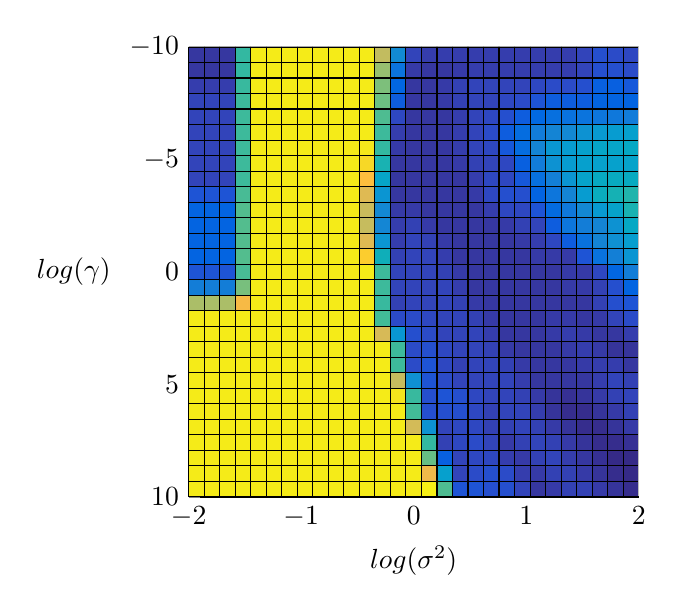
\begin{tikzpicture}

\begin{axis}[%
width=2.25in,
height=2.25in,
at={(0.631944in,0.48125in)},
scale only axis,
xmin=-10,
xmax=10,
xlabel={$log(\gamma)$},
xmajorgrids,
ymin=-2,
ymax=2,
ylabel={$log(\sigma^2)$},
ymajorgrids,
zmin=0,
zmax=0.4,
zmajorgrids,
view={90}{90},
axis x line*=bottom,
axis y line*=left,
axis z line*=left
]

\addplot3[%
surf,
faceted color=black,
shader=faceted,
colormap={mymap}{[1pt] rgb(0pt)=(0.2081,0.1663,0.5292); rgb(1pt)=(0.211624,0.189781,0.577676); rgb(2pt)=(0.212252,0.213771,0.626971); rgb(3pt)=(0.2081,0.2386,0.677086); rgb(4pt)=(0.195905,0.264457,0.7279); rgb(5pt)=(0.170729,0.291938,0.779248); rgb(6pt)=(0.125271,0.324243,0.830271); rgb(7pt)=(0.0591333,0.359833,0.868333); rgb(8pt)=(0.0116952,0.38751,0.881957); rgb(9pt)=(0.00595714,0.408614,0.882843); rgb(10pt)=(0.0165143,0.4266,0.878633); rgb(11pt)=(0.0328524,0.443043,0.871957); rgb(12pt)=(0.0498143,0.458571,0.864057); rgb(13pt)=(0.0629333,0.47369,0.855438); rgb(14pt)=(0.0722667,0.488667,0.8467); rgb(15pt)=(0.0779429,0.503986,0.838371); rgb(16pt)=(0.0793476,0.520024,0.831181); rgb(17pt)=(0.0749429,0.537543,0.826271); rgb(18pt)=(0.0640571,0.556986,0.823957); rgb(19pt)=(0.0487714,0.577224,0.822829); rgb(20pt)=(0.0343429,0.596581,0.819852); rgb(21pt)=(0.0265,0.6137,0.8135); rgb(22pt)=(0.0238905,0.628662,0.803762); rgb(23pt)=(0.0230905,0.641786,0.791267); rgb(24pt)=(0.0227714,0.653486,0.776757); rgb(25pt)=(0.0266619,0.664195,0.760719); rgb(26pt)=(0.0383714,0.674271,0.743552); rgb(27pt)=(0.0589714,0.683757,0.725386); rgb(28pt)=(0.0843,0.692833,0.706167); rgb(29pt)=(0.113295,0.7015,0.685857); rgb(30pt)=(0.145271,0.709757,0.664629); rgb(31pt)=(0.180133,0.717657,0.642433); rgb(32pt)=(0.217829,0.725043,0.619262); rgb(33pt)=(0.258643,0.731714,0.595429); rgb(34pt)=(0.302171,0.737605,0.571186); rgb(35pt)=(0.348167,0.742433,0.547267); rgb(36pt)=(0.395257,0.7459,0.524443); rgb(37pt)=(0.44201,0.748081,0.503314); rgb(38pt)=(0.487124,0.749062,0.483976); rgb(39pt)=(0.530029,0.749114,0.466114); rgb(40pt)=(0.570857,0.748519,0.44939); rgb(41pt)=(0.609852,0.747314,0.433686); rgb(42pt)=(0.6473,0.7456,0.4188); rgb(43pt)=(0.683419,0.743476,0.404433); rgb(44pt)=(0.71841,0.741133,0.390476); rgb(45pt)=(0.752486,0.7384,0.376814); rgb(46pt)=(0.785843,0.735567,0.363271); rgb(47pt)=(0.818505,0.732733,0.34979); rgb(48pt)=(0.850657,0.7299,0.336029); rgb(49pt)=(0.882433,0.727433,0.3217); rgb(50pt)=(0.913933,0.725786,0.306276); rgb(51pt)=(0.944957,0.726114,0.288643); rgb(52pt)=(0.973895,0.731395,0.266648); rgb(53pt)=(0.993771,0.745457,0.240348); rgb(54pt)=(0.999043,0.765314,0.216414); rgb(55pt)=(0.995533,0.786057,0.196652); rgb(56pt)=(0.988,0.8066,0.179367); rgb(57pt)=(0.978857,0.827143,0.163314); rgb(58pt)=(0.9697,0.848138,0.147452); rgb(59pt)=(0.962586,0.870514,0.1309); rgb(60pt)=(0.958871,0.8949,0.113243); rgb(61pt)=(0.959824,0.921833,0.0948381); rgb(62pt)=(0.9661,0.951443,0.0755333); rgb(63pt)=(0.9763,0.9831,0.0538)},
mesh/rows=30]
table[row sep=crcr,header=false] {%
%
-10	-2	0.04\\
-10	-1.86206896551724	0.04\\
-10	-1.72413793103448	0.04\\
-10	-1.58620689655172	0.04\\
-10	-1.44827586206897	0.33\\
-10	-1.31034482758621	0.33\\
-10	-1.17241379310345	0.33\\
-10	-1.03448275862069	0.33\\
-10	-0.896551724137931	0.33\\
-10	-0.758620689655172	0.33\\
-10	-0.620689655172414	0.33\\
-10	-0.482758620689655	0.33\\
-10	-0.344827586206897	0.33\\
-10	-0.206896551724138	0.2\\
-10	-0.0689655172413792	0.06\\
-10	0.0689655172413794	0.05\\
-10	0.206896551724138	0.05\\
-10	0.344827586206896	0.05\\
-10	0.482758620689655	0.05\\
-10	0.620689655172414	0.05\\
-10	0.758620689655173	0.05\\
-10	0.896551724137931	0.05\\
-10	1.03448275862069	0.05\\
-10	1.17241379310345	0.05\\
-10	1.31034482758621	0.05\\
-10	1.44827586206897	0.05\\
-10	1.58620689655172	0.06\\
-10	1.72413793103448	0.07\\
-10	1.86206896551724	0.05\\
-10	2	0.06\\
-9.31034482758621	-2	0.04\\
-9.31034482758621	-1.86206896551724	0.04\\
-9.31034482758621	-1.72413793103448	0.04\\
-9.31034482758621	-1.58620689655172	0.04\\
-9.31034482758621	-1.44827586206897	0.33\\
-9.31034482758621	-1.31034482758621	0.33\\
-9.31034482758621	-1.17241379310345	0.33\\
-9.31034482758621	-1.03448275862069	0.33\\
-9.31034482758621	-0.896551724137931	0.33\\
-9.31034482758621	-0.758620689655172	0.33\\
-9.31034482758621	-0.620689655172414	0.33\\
-9.31034482758621	-0.482758620689655	0.33\\
-9.31034482758621	-0.344827586206897	0.33\\
-9.31034482758621	-0.206896551724138	0.15\\
-9.31034482758621	-0.0689655172413792	0.05\\
-9.31034482758621	0.0689655172413794	0.04\\
-9.31034482758621	0.206896551724138	0.04\\
-9.31034482758621	0.344827586206896	0.04\\
-9.31034482758621	0.482758620689655	0.04\\
-9.31034482758621	0.620689655172414	0.04\\
-9.31034482758621	0.758620689655173	0.04\\
-9.31034482758621	0.896551724137931	0.04\\
-9.31034482758621	1.03448275862069	0.04\\
-9.31034482758621	1.17241379310345	0.04\\
-9.31034482758621	1.31034482758621	0.04\\
-9.31034482758621	1.44827586206897	0.04\\
-9.31034482758621	1.58620689655172	0.05\\
-9.31034482758621	1.72413793103448	0.05\\
-9.31034482758621	1.86206896551724	0.05\\
-9.31034482758621	2	0.05\\
-8.62068965517241	-2	0.04\\
-8.62068965517241	-1.86206896551724	0.04\\
-8.62068965517241	-1.72413793103448	0.04\\
-8.62068965517241	-1.58620689655172	0.04\\
-8.62068965517241	-1.44827586206897	0.33\\
-8.62068965517241	-1.31034482758621	0.33\\
-8.62068965517241	-1.17241379310345	0.33\\
-8.62068965517241	-1.03448275862069	0.33\\
-8.62068965517241	-0.896551724137931	0.33\\
-8.62068965517241	-0.758620689655172	0.33\\
-8.62068965517241	-0.620689655172414	0.33\\
-8.62068965517241	-0.482758620689655	0.33\\
-8.62068965517241	-0.344827586206897	0.33\\
-8.62068965517241	-0.206896551724138	0.11\\
-8.62068965517241	-0.0689655172413792	0.04\\
-8.62068965517241	0.0689655172413794	0.04\\
-8.62068965517241	0.206896551724138	0.04\\
-8.62068965517241	0.344827586206896	0.04\\
-8.62068965517241	0.482758620689655	0.05\\
-8.62068965517241	0.620689655172414	0.05\\
-8.62068965517241	0.758620689655173	0.05\\
-8.62068965517241	0.896551724137931	0.05\\
-8.62068965517241	1.03448275862069	0.05\\
-8.62068965517241	1.17241379310345	0.05\\
-8.62068965517241	1.31034482758621	0.05\\
-8.62068965517241	1.44827586206897	0.05\\
-8.62068965517241	1.58620689655172	0.06\\
-8.62068965517241	1.72413793103448	0.07\\
-8.62068965517241	1.86206896551724	0.06\\
-8.62068965517241	2	0.06\\
-7.93103448275862	-2	0.05\\
-7.93103448275862	-1.86206896551724	0.05\\
-7.93103448275862	-1.72413793103448	0.05\\
-7.93103448275862	-1.58620689655172	0.05\\
-7.93103448275862	-1.44827586206897	0.33\\
-7.93103448275862	-1.31034482758621	0.33\\
-7.93103448275862	-1.17241379310345	0.33\\
-7.93103448275862	-1.03448275862069	0.33\\
-7.93103448275862	-0.896551724137931	0.33\\
-7.93103448275862	-0.758620689655172	0.33\\
-7.93103448275862	-0.620689655172414	0.33\\
-7.93103448275862	-0.482758620689655	0.33\\
-7.93103448275862	-0.344827586206897	0.33\\
-7.93103448275862	-0.206896551724138	0.1\\
-7.93103448275862	-0.0689655172413792	0.04\\
-7.93103448275862	0.0689655172413794	0.04\\
-7.93103448275862	0.206896551724138	0.04\\
-7.93103448275862	0.344827586206896	0.05\\
-7.93103448275862	0.482758620689655	0.05\\
-7.93103448275862	0.620689655172414	0.05\\
-7.93103448275862	0.758620689655173	0.05\\
-7.93103448275862	0.896551724137931	0.05\\
-7.93103448275862	1.03448275862069	0.05\\
-7.93103448275862	1.17241379310345	0.06\\
-7.93103448275862	1.31034482758621	0.06\\
-7.93103448275862	1.44827586206897	0.06\\
-7.93103448275862	1.58620689655172	0.06\\
-7.93103448275862	1.72413793103448	0.08\\
-7.93103448275862	1.86206896551724	0.06\\
-7.93103448275862	2	0.07\\
-7.24137931034483	-2	0.05\\
-7.24137931034483	-1.86206896551724	0.05\\
-7.24137931034483	-1.72413793103448	0.05\\
-7.24137931034483	-1.58620689655172	0.05\\
-7.24137931034483	-1.44827586206897	0.33\\
-7.24137931034483	-1.31034482758621	0.33\\
-7.24137931034483	-1.17241379310345	0.33\\
-7.24137931034483	-1.03448275862069	0.33\\
-7.24137931034483	-0.896551724137931	0.33\\
-7.24137931034483	-0.758620689655172	0.33\\
-7.24137931034483	-0.620689655172414	0.33\\
-7.24137931034483	-0.482758620689655	0.33\\
-7.24137931034483	-0.344827586206897	0.33\\
-7.24137931034483	-0.206896551724138	0.08\\
-7.24137931034483	-0.0689655172413792	0.04\\
-7.24137931034483	0.0689655172413794	0.04\\
-7.24137931034483	0.206896551724138	0.04\\
-7.24137931034483	0.344827586206896	0.04\\
-7.24137931034483	0.482758620689655	0.05\\
-7.24137931034483	0.620689655172414	0.05\\
-7.24137931034483	0.758620689655173	0.05\\
-7.24137931034483	0.896551724137931	0.06\\
-7.24137931034483	1.03448275862069	0.06\\
-7.24137931034483	1.17241379310345	0.07\\
-7.24137931034483	1.31034482758621	0.07\\
-7.24137931034483	1.44827586206897	0.07\\
-7.24137931034483	1.58620689655172	0.07\\
-7.24137931034483	1.72413793103448	0.07\\
-7.24137931034483	1.86206896551724	0.07\\
-7.24137931034483	2	0.08\\
-6.55172413793103	-2	0.05\\
-6.55172413793103	-1.86206896551724	0.05\\
-6.55172413793103	-1.72413793103448	0.05\\
-6.55172413793103	-1.58620689655172	0.05\\
-6.55172413793103	-1.44827586206897	0.33\\
-6.55172413793103	-1.31034482758621	0.33\\
-6.55172413793103	-1.17241379310345	0.33\\
-6.55172413793103	-1.03448275862069	0.33\\
-6.55172413793103	-0.896551724137931	0.33\\
-6.55172413793103	-0.758620689655172	0.33\\
-6.55172413793103	-0.620689655172414	0.33\\
-6.55172413793103	-0.482758620689655	0.33\\
-6.55172413793103	-0.344827586206897	0.33\\
-6.55172413793103	-0.206896551724138	0.05\\
-6.55172413793103	-0.0689655172413792	0.04\\
-6.55172413793103	0.0689655172413794	0.04\\
-6.55172413793103	0.206896551724138	0.04\\
-6.55172413793103	0.344827586206896	0.04\\
-6.55172413793103	0.482758620689655	0.05\\
-6.55172413793103	0.620689655172414	0.05\\
-6.55172413793103	0.758620689655173	0.06\\
-6.55172413793103	0.896551724137931	0.06\\
-6.55172413793103	1.03448275862069	0.08\\
-6.55172413793103	1.17241379310345	0.09\\
-6.55172413793103	1.31034482758621	0.1\\
-6.55172413793103	1.44827586206897	0.1\\
-6.55172413793103	1.58620689655172	0.11\\
-6.55172413793103	1.72413793103448	0.11\\
-6.55172413793103	1.86206896551724	0.12\\
-6.55172413793103	2	0.12\\
-5.86206896551724	-2	0.05\\
-5.86206896551724	-1.86206896551724	0.05\\
-5.86206896551724	-1.72413793103448	0.05\\
-5.86206896551724	-1.58620689655172	0.05\\
-5.86206896551724	-1.44827586206897	0.33\\
-5.86206896551724	-1.31034482758621	0.33\\
-5.86206896551724	-1.17241379310345	0.33\\
-5.86206896551724	-1.03448275862069	0.33\\
-5.86206896551724	-0.896551724137931	0.33\\
-5.86206896551724	-0.758620689655172	0.33\\
-5.86206896551724	-0.620689655172414	0.33\\
-5.86206896551724	-0.482758620689655	0.33\\
-5.86206896551724	-0.344827586206897	0.33\\
-5.86206896551724	-0.206896551724138	0.05\\
-5.86206896551724	-0.0689655172413792	0.04\\
-5.86206896551724	0.0689655172413794	0.04\\
-5.86206896551724	0.206896551724138	0.04\\
-5.86206896551724	0.344827586206896	0.04\\
-5.86206896551724	0.482758620689655	0.05\\
-5.86206896551724	0.620689655172414	0.05\\
-5.86206896551724	0.758620689655173	0.06\\
-5.86206896551724	0.896551724137931	0.08\\
-5.86206896551724	1.03448275862069	0.1\\
-5.86206896551724	1.17241379310345	0.12\\
-5.86206896551724	1.31034482758621	0.12\\
-5.86206896551724	1.44827586206897	0.13\\
-5.86206896551724	1.58620689655172	0.15\\
-5.86206896551724	1.72413793103448	0.15\\
-5.86206896551724	1.86206896551724	0.15\\
-5.86206896551724	2	0.16\\
-5.17241379310345	-2	0.05\\
-5.17241379310345	-1.86206896551724	0.05\\
-5.17241379310345	-1.72413793103448	0.05\\
-5.17241379310345	-1.58620689655172	0.05\\
-5.17241379310345	-1.44827586206897	0.33\\
-5.17241379310345	-1.31034482758621	0.33\\
-5.17241379310345	-1.17241379310345	0.33\\
-5.17241379310345	-1.03448275862069	0.33\\
-5.17241379310345	-0.896551724137931	0.33\\
-5.17241379310345	-0.758620689655172	0.33\\
-5.17241379310345	-0.620689655172414	0.33\\
-5.17241379310345	-0.482758620689655	0.33\\
-5.17241379310345	-0.344827586206897	0.32\\
-5.17241379310345	-0.206896551724138	0.04\\
-5.17241379310345	-0.0689655172413792	0.04\\
-5.17241379310345	0.0689655172413794	0.04\\
-5.17241379310345	0.206896551724138	0.04\\
-5.17241379310345	0.344827586206896	0.04\\
-5.17241379310345	0.482758620689655	0.05\\
-5.17241379310345	0.620689655172414	0.05\\
-5.17241379310345	0.758620689655173	0.05\\
-5.17241379310345	0.896551724137931	0.06\\
-5.17241379310345	1.03448275862069	0.08\\
-5.17241379310345	1.17241379310345	0.13\\
-5.17241379310345	1.31034482758621	0.14\\
-5.17241379310345	1.44827586206897	0.14\\
-5.17241379310345	1.58620689655172	0.14\\
-5.17241379310345	1.72413793103448	0.14\\
-5.17241379310345	1.86206896551724	0.14\\
-5.17241379310345	2	0.15\\
-4.48275862068965	-2	0.05\\
-4.48275862068965	-1.86206896551724	0.05\\
-4.48275862068965	-1.72413793103448	0.05\\
-4.48275862068965	-1.58620689655172	0.05\\
-4.48275862068965	-1.44827586206897	0.33\\
-4.48275862068965	-1.31034482758621	0.33\\
-4.48275862068965	-1.17241379310345	0.33\\
-4.48275862068965	-1.03448275862069	0.33\\
-4.48275862068965	-0.896551724137931	0.33\\
-4.48275862068965	-0.758620689655172	0.33\\
-4.48275862068965	-0.620689655172414	0.33\\
-4.48275862068965	-0.482758620689655	0.33\\
-4.48275862068965	-0.344827586206897	0.28\\
-4.48275862068965	-0.206896551724138	0.04\\
-4.48275862068965	-0.0689655172413792	0.04\\
-4.48275862068965	0.0689655172413794	0.04\\
-4.48275862068965	0.206896551724138	0.04\\
-4.48275862068965	0.344827586206896	0.04\\
-4.48275862068965	0.482758620689655	0.04\\
-4.48275862068965	0.620689655172414	0.05\\
-4.48275862068965	0.758620689655173	0.05\\
-4.48275862068965	0.896551724137931	0.05\\
-4.48275862068965	1.03448275862069	0.08\\
-4.48275862068965	1.17241379310345	0.1\\
-4.48275862068965	1.31034482758621	0.12\\
-4.48275862068965	1.44827586206897	0.13\\
-4.48275862068965	1.58620689655172	0.14\\
-4.48275862068965	1.72413793103448	0.14\\
-4.48275862068965	1.86206896551724	0.14\\
-4.48275862068965	2	0.14\\
-3.79310344827586	-2	0.05\\
-3.79310344827586	-1.86206896551724	0.05\\
-3.79310344827586	-1.72413793103448	0.05\\
-3.79310344827586	-1.58620689655172	0.05\\
-3.79310344827586	-1.44827586206897	0.33\\
-3.79310344827586	-1.31034482758621	0.33\\
-3.79310344827586	-1.17241379310345	0.33\\
-3.79310344827586	-1.03448275862069	0.33\\
-3.79310344827586	-0.896551724137931	0.33\\
-3.79310344827586	-0.758620689655172	0.33\\
-3.79310344827586	-0.620689655172414	0.33\\
-3.79310344827586	-0.482758620689655	0.33\\
-3.79310344827586	-0.344827586206897	0.22\\
-3.79310344827586	-0.206896551724138	0.04\\
-3.79310344827586	-0.0689655172413792	0.04\\
-3.79310344827586	0.0689655172413794	0.04\\
-3.79310344827586	0.206896551724138	0.04\\
-3.79310344827586	0.344827586206896	0.04\\
-3.79310344827586	0.482758620689655	0.04\\
-3.79310344827586	0.620689655172414	0.05\\
-3.79310344827586	0.758620689655173	0.06\\
-3.79310344827586	0.896551724137931	0.05\\
-3.79310344827586	1.03448275862069	0.07\\
-3.79310344827586	1.17241379310345	0.08\\
-3.79310344827586	1.31034482758621	0.11\\
-3.79310344827586	1.44827586206897	0.14\\
-3.79310344827586	1.58620689655172	0.16\\
-3.79310344827586	1.72413793103448	0.17\\
-3.79310344827586	1.86206896551724	0.17\\
-3.79310344827586	2	0.17\\
-3.10344827586207	-2	0.07\\
-3.10344827586207	-1.86206896551724	0.07\\
-3.10344827586207	-1.72413793103448	0.07\\
-3.10344827586207	-1.58620689655172	0.07\\
-3.10344827586207	-1.44827586206897	0.33\\
-3.10344827586207	-1.31034482758621	0.33\\
-3.10344827586207	-1.17241379310345	0.33\\
-3.10344827586207	-1.03448275862069	0.33\\
-3.10344827586207	-0.896551724137931	0.33\\
-3.10344827586207	-0.758620689655172	0.33\\
-3.10344827586207	-0.620689655172414	0.33\\
-3.10344827586207	-0.482758620689655	0.33\\
-3.10344827586207	-0.344827586206897	0.2\\
-3.10344827586207	-0.206896551724138	0.04\\
-3.10344827586207	-0.0689655172413792	0.04\\
-3.10344827586207	0.0689655172413794	0.04\\
-3.10344827586207	0.206896551724138	0.04\\
-3.10344827586207	0.344827586206896	0.04\\
-3.10344827586207	0.482758620689655	0.04\\
-3.10344827586207	0.620689655172414	0.04\\
-3.10344827586207	0.758620689655173	0.06\\
-3.10344827586207	0.896551724137931	0.06\\
-3.10344827586207	1.03448275862069	0.05\\
-3.10344827586207	1.17241379310345	0.08\\
-3.10344827586207	1.31034482758621	0.09\\
-3.10344827586207	1.44827586206897	0.09\\
-3.10344827586207	1.58620689655172	0.14\\
-3.10344827586207	1.72413793103448	0.16\\
-3.10344827586207	1.86206896551724	0.17\\
-3.10344827586207	2	0.19\\
-2.41379310344828	-2	0.07\\
-2.41379310344828	-1.86206896551724	0.07\\
-2.41379310344828	-1.72413793103448	0.07\\
-2.41379310344828	-1.58620689655172	0.07\\
-2.41379310344828	-1.44827586206897	0.33\\
-2.41379310344828	-1.31034482758621	0.33\\
-2.41379310344828	-1.17241379310345	0.33\\
-2.41379310344828	-1.03448275862069	0.33\\
-2.41379310344828	-0.896551724137931	0.33\\
-2.41379310344828	-0.758620689655172	0.33\\
-2.41379310344828	-0.620689655172414	0.33\\
-2.41379310344828	-0.482758620689655	0.33\\
-2.41379310344828	-0.344827586206897	0.17\\
-2.41379310344828	-0.206896551724138	0.04\\
-2.41379310344828	-0.0689655172413792	0.05\\
-2.41379310344828	0.0689655172413794	0.04\\
-2.41379310344828	0.206896551724138	0.04\\
-2.41379310344828	0.344827586206896	0.04\\
-2.41379310344828	0.482758620689655	0.04\\
-2.41379310344828	0.620689655172414	0.04\\
-2.41379310344828	0.758620689655173	0.04\\
-2.41379310344828	0.896551724137931	0.05\\
-2.41379310344828	1.03448275862069	0.05\\
-2.41379310344828	1.17241379310345	0.06\\
-2.41379310344828	1.31034482758621	0.08\\
-2.41379310344828	1.44827586206897	0.11\\
-2.41379310344828	1.58620689655172	0.11\\
-2.41379310344828	1.72413793103448	0.11\\
-2.41379310344828	1.86206896551724	0.13\\
-2.41379310344828	2	0.19\\
-1.72413793103448	-2	0.07\\
-1.72413793103448	-1.86206896551724	0.07\\
-1.72413793103448	-1.72413793103448	0.07\\
-1.72413793103448	-1.58620689655172	0.07\\
-1.72413793103448	-1.44827586206897	0.33\\
-1.72413793103448	-1.31034482758621	0.33\\
-1.72413793103448	-1.17241379310345	0.33\\
-1.72413793103448	-1.03448275862069	0.33\\
-1.72413793103448	-0.896551724137931	0.33\\
-1.72413793103448	-0.758620689655172	0.33\\
-1.72413793103448	-0.620689655172414	0.33\\
-1.72413793103448	-0.482758620689655	0.33\\
-1.72413793103448	-0.344827586206897	0.19\\
-1.72413793103448	-0.206896551724138	0.04\\
-1.72413793103448	-0.0689655172413792	0.05\\
-1.72413793103448	0.0689655172413794	0.05\\
-1.72413793103448	0.206896551724138	0.04\\
-1.72413793103448	0.344827586206896	0.04\\
-1.72413793103448	0.482758620689655	0.04\\
-1.72413793103448	0.620689655172414	0.04\\
-1.72413793103448	0.758620689655173	0.04\\
-1.72413793103448	0.896551724137931	0.04\\
-1.72413793103448	1.03448275862069	0.05\\
-1.72413793103448	1.17241379310345	0.04\\
-1.72413793103448	1.31034482758621	0.08\\
-1.72413793103448	1.44827586206897	0.09\\
-1.72413793103448	1.58620689655172	0.09\\
-1.72413793103448	1.72413793103448	0.12\\
-1.72413793103448	1.86206896551724	0.13\\
-1.72413793103448	2	0.15\\
-1.03448275862069	-2	0.07\\
-1.03448275862069	-1.86206896551724	0.07\\
-1.03448275862069	-1.72413793103448	0.07\\
-1.03448275862069	-1.58620689655172	0.07\\
-1.03448275862069	-1.44827586206897	0.33\\
-1.03448275862069	-1.31034482758621	0.33\\
-1.03448275862069	-1.17241379310345	0.33\\
-1.03448275862069	-1.03448275862069	0.33\\
-1.03448275862069	-0.896551724137931	0.33\\
-1.03448275862069	-0.758620689655172	0.33\\
-1.03448275862069	-0.620689655172414	0.33\\
-1.03448275862069	-0.482758620689655	0.33\\
-1.03448275862069	-0.344827586206897	0.23\\
-1.03448275862069	-0.206896551724138	0.04\\
-1.03448275862069	-0.0689655172413792	0.05\\
-1.03448275862069	0.0689655172413794	0.05\\
-1.03448275862069	0.206896551724138	0.05\\
-1.03448275862069	0.344827586206896	0.04\\
-1.03448275862069	0.482758620689655	0.04\\
-1.03448275862069	0.620689655172414	0.04\\
-1.03448275862069	0.758620689655173	0.04\\
-1.03448275862069	0.896551724137931	0.04\\
-1.03448275862069	1.03448275862069	0.04\\
-1.03448275862069	1.17241379310345	0.05\\
-1.03448275862069	1.31034482758621	0.04\\
-1.03448275862069	1.44827586206897	0.05\\
-1.03448275862069	1.58620689655172	0.11\\
-1.03448275862069	1.72413793103448	0.11\\
-1.03448275862069	1.86206896551724	0.12\\
-1.03448275862069	2	0.14\\
-0.344827586206897	-2	0.07\\
-0.344827586206897	-1.86206896551724	0.07\\
-0.344827586206897	-1.72413793103448	0.07\\
-0.344827586206897	-1.58620689655172	0.07\\
-0.344827586206897	-1.44827586206897	0.33\\
-0.344827586206897	-1.31034482758621	0.33\\
-0.344827586206897	-1.17241379310345	0.33\\
-0.344827586206897	-1.03448275862069	0.33\\
-0.344827586206897	-0.896551724137931	0.33\\
-0.344827586206897	-0.758620689655172	0.33\\
-0.344827586206897	-0.620689655172414	0.33\\
-0.344827586206897	-0.482758620689655	0.33\\
-0.344827586206897	-0.344827586206897	0.33\\
-0.344827586206897	-0.206896551724138	0.05\\
-0.344827586206897	-0.0689655172413792	0.05\\
-0.344827586206897	0.0689655172413794	0.05\\
-0.344827586206897	0.206896551724138	0.05\\
-0.344827586206897	0.344827586206896	0.04\\
-0.344827586206897	0.482758620689655	0.04\\
-0.344827586206897	0.620689655172414	0.04\\
-0.344827586206897	0.758620689655173	0.04\\
-0.344827586206897	0.896551724137931	0.04\\
-0.344827586206897	1.03448275862069	0.04\\
-0.344827586206897	1.17241379310345	0.04\\
-0.344827586206897	1.31034482758621	0.04\\
-0.344827586206897	1.44827586206897	0.04\\
-0.344827586206897	1.58620689655172	0.04\\
-0.344827586206897	1.72413793103448	0.08\\
-0.344827586206897	1.86206896551724	0.1\\
-0.344827586206897	2	0.14\\
0.344827586206897	-2	0.05\\
0.344827586206897	-1.86206896551724	0.05\\
0.344827586206897	-1.72413793103448	0.05\\
0.344827586206897	-1.58620689655172	0.05\\
0.344827586206897	-1.44827586206897	0.33\\
0.344827586206897	-1.31034482758621	0.33\\
0.344827586206897	-1.17241379310345	0.33\\
0.344827586206897	-1.03448275862069	0.33\\
0.344827586206897	-0.896551724137931	0.33\\
0.344827586206897	-0.758620689655172	0.33\\
0.344827586206897	-0.620689655172414	0.33\\
0.344827586206897	-0.482758620689655	0.33\\
0.344827586206897	-0.344827586206897	0.33\\
0.344827586206897	-0.206896551724138	0.05\\
0.344827586206897	-0.0689655172413792	0.05\\
0.344827586206897	0.0689655172413794	0.05\\
0.344827586206897	0.206896551724138	0.05\\
0.344827586206897	0.344827586206896	0.05\\
0.344827586206897	0.482758620689655	0.04\\
0.344827586206897	0.620689655172414	0.04\\
0.344827586206897	0.758620689655173	0.04\\
0.344827586206897	0.896551724137931	0.04\\
0.344827586206897	1.03448275862069	0.04\\
0.344827586206897	1.17241379310345	0.04\\
0.344827586206897	1.31034482758621	0.04\\
0.344827586206897	1.44827586206897	0.05\\
0.344827586206897	1.58620689655172	0.04\\
0.344827586206897	1.72413793103448	0.05\\
0.344827586206897	1.86206896551724	0.06\\
0.344827586206897	2	0.1\\
1.03448275862069	-2	0.15\\
1.03448275862069	-1.86206896551724	0.15\\
1.03448275862069	-1.72413793103448	0.15\\
1.03448275862069	-1.58620689655172	0.15\\
1.03448275862069	-1.44827586206897	0.33\\
1.03448275862069	-1.31034482758621	0.33\\
1.03448275862069	-1.17241379310345	0.33\\
1.03448275862069	-1.03448275862069	0.33\\
1.03448275862069	-0.896551724137931	0.33\\
1.03448275862069	-0.758620689655172	0.33\\
1.03448275862069	-0.620689655172414	0.33\\
1.03448275862069	-0.482758620689655	0.33\\
1.03448275862069	-0.344827586206897	0.33\\
1.03448275862069	-0.206896551724138	0.05\\
1.03448275862069	-0.0689655172413792	0.05\\
1.03448275862069	0.0689655172413794	0.05\\
1.03448275862069	0.206896551724138	0.05\\
1.03448275862069	0.344827586206896	0.05\\
1.03448275862069	0.482758620689655	0.04\\
1.03448275862069	0.620689655172414	0.04\\
1.03448275862069	0.758620689655173	0.04\\
1.03448275862069	0.896551724137931	0.04\\
1.03448275862069	1.03448275862069	0.04\\
1.03448275862069	1.17241379310345	0.04\\
1.03448275862069	1.31034482758621	0.04\\
1.03448275862069	1.44827586206897	0.04\\
1.03448275862069	1.58620689655172	0.04\\
1.03448275862069	1.72413793103448	0.06\\
1.03448275862069	1.86206896551724	0.06\\
1.03448275862069	2	0.06\\
1.72413793103448	-2	0.33\\
1.72413793103448	-1.86206896551724	0.33\\
1.72413793103448	-1.72413793103448	0.33\\
1.72413793103448	-1.58620689655172	0.33\\
1.72413793103448	-1.44827586206897	0.33\\
1.72413793103448	-1.31034482758621	0.33\\
1.72413793103448	-1.17241379310345	0.33\\
1.72413793103448	-1.03448275862069	0.33\\
1.72413793103448	-0.896551724137931	0.33\\
1.72413793103448	-0.758620689655172	0.33\\
1.72413793103448	-0.620689655172414	0.33\\
1.72413793103448	-0.482758620689655	0.33\\
1.72413793103448	-0.344827586206897	0.33\\
1.72413793103448	-0.206896551724138	0.04\\
1.72413793103448	-0.0689655172413792	0.05\\
1.72413793103448	0.0689655172413794	0.05\\
1.72413793103448	0.206896551724138	0.05\\
1.72413793103448	0.344827586206896	0.05\\
1.72413793103448	0.482758620689655	0.05\\
1.72413793103448	0.620689655172414	0.04\\
1.72413793103448	0.758620689655173	0.04\\
1.72413793103448	0.896551724137931	0.04\\
1.72413793103448	1.03448275862069	0.04\\
1.72413793103448	1.17241379310345	0.04\\
1.72413793103448	1.31034482758621	0.04\\
1.72413793103448	1.44827586206897	0.04\\
1.72413793103448	1.58620689655172	0.04\\
1.72413793103448	1.72413793103448	0.05\\
1.72413793103448	1.86206896551724	0.06\\
1.72413793103448	2	0.06\\
2.41379310344828	-2	0.33\\
2.41379310344828	-1.86206896551724	0.33\\
2.41379310344828	-1.72413793103448	0.33\\
2.41379310344828	-1.58620689655172	0.33\\
2.41379310344828	-1.44827586206897	0.33\\
2.41379310344828	-1.31034482758621	0.33\\
2.41379310344828	-1.17241379310345	0.33\\
2.41379310344828	-1.03448275862069	0.33\\
2.41379310344828	-0.896551724137931	0.33\\
2.41379310344828	-0.758620689655172	0.33\\
2.41379310344828	-0.620689655172414	0.33\\
2.41379310344828	-0.482758620689655	0.33\\
2.41379310344828	-0.344827586206897	0.33\\
2.41379310344828	-0.206896551724138	0.07\\
2.41379310344828	-0.0689655172413792	0.06\\
2.41379310344828	0.0689655172413794	0.06\\
2.41379310344828	0.206896551724138	0.05\\
2.41379310344828	0.344827586206896	0.05\\
2.41379310344828	0.482758620689655	0.05\\
2.41379310344828	0.620689655172414	0.05\\
2.41379310344828	0.758620689655173	0.04\\
2.41379310344828	0.896551724137931	0.04\\
2.41379310344828	1.03448275862069	0.04\\
2.41379310344828	1.17241379310345	0.04\\
2.41379310344828	1.31034482758621	0.05\\
2.41379310344828	1.44827586206897	0.04\\
2.41379310344828	1.58620689655172	0.04\\
2.41379310344828	1.72413793103448	0.04\\
2.41379310344828	1.86206896551724	0.05\\
2.41379310344828	2	0.05\\
3.10344827586207	-2	0.33\\
3.10344827586207	-1.86206896551724	0.33\\
3.10344827586207	-1.72413793103448	0.33\\
3.10344827586207	-1.58620689655172	0.33\\
3.10344827586207	-1.44827586206897	0.33\\
3.10344827586207	-1.31034482758621	0.33\\
3.10344827586207	-1.17241379310345	0.33\\
3.10344827586207	-1.03448275862069	0.33\\
3.10344827586207	-0.896551724137931	0.33\\
3.10344827586207	-0.758620689655172	0.33\\
3.10344827586207	-0.620689655172414	0.33\\
3.10344827586207	-0.482758620689655	0.33\\
3.10344827586207	-0.344827586206897	0.33\\
3.10344827586207	-0.206896551724138	0.33\\
3.10344827586207	-0.0689655172413792	0.05\\
3.10344827586207	0.0689655172413794	0.06\\
3.10344827586207	0.206896551724138	0.05\\
3.10344827586207	0.344827586206896	0.05\\
3.10344827586207	0.482758620689655	0.05\\
3.10344827586207	0.620689655172414	0.05\\
3.10344827586207	0.758620689655173	0.04\\
3.10344827586207	0.896551724137931	0.04\\
3.10344827586207	1.03448275862069	0.04\\
3.10344827586207	1.17241379310345	0.04\\
3.10344827586207	1.31034482758621	0.04\\
3.10344827586207	1.44827586206897	0.05\\
3.10344827586207	1.58620689655172	0.04\\
3.10344827586207	1.72413793103448	0.04\\
3.10344827586207	1.86206896551724	0.03\\
3.10344827586207	2	0.05\\
3.79310344827586	-2	0.33\\
3.79310344827586	-1.86206896551724	0.33\\
3.79310344827586	-1.72413793103448	0.33\\
3.79310344827586	-1.58620689655172	0.33\\
3.79310344827586	-1.44827586206897	0.33\\
3.79310344827586	-1.31034482758621	0.33\\
3.79310344827586	-1.17241379310345	0.33\\
3.79310344827586	-1.03448275862069	0.33\\
3.79310344827586	-0.896551724137931	0.33\\
3.79310344827586	-0.758620689655172	0.33\\
3.79310344827586	-0.620689655172414	0.33\\
3.79310344827586	-0.482758620689655	0.33\\
3.79310344827586	-0.344827586206897	0.33\\
3.79310344827586	-0.206896551724138	0.33\\
3.79310344827586	-0.0689655172413792	0.05\\
3.79310344827586	0.0689655172413794	0.06\\
3.79310344827586	0.206896551724138	0.06\\
3.79310344827586	0.344827586206896	0.05\\
3.79310344827586	0.482758620689655	0.05\\
3.79310344827586	0.620689655172414	0.05\\
3.79310344827586	0.758620689655173	0.05\\
3.79310344827586	0.896551724137931	0.04\\
3.79310344827586	1.03448275862069	0.04\\
3.79310344827586	1.17241379310345	0.04\\
3.79310344827586	1.31034482758621	0.04\\
3.79310344827586	1.44827586206897	0.04\\
3.79310344827586	1.58620689655172	0.05\\
3.79310344827586	1.72413793103448	0.04\\
3.79310344827586	1.86206896551724	0.04\\
3.79310344827586	2	0.03\\
4.48275862068965	-2	0.33\\
4.48275862068965	-1.86206896551724	0.33\\
4.48275862068965	-1.72413793103448	0.33\\
4.48275862068965	-1.58620689655172	0.33\\
4.48275862068965	-1.44827586206897	0.33\\
4.48275862068965	-1.31034482758621	0.33\\
4.48275862068965	-1.17241379310345	0.33\\
4.48275862068965	-1.03448275862069	0.33\\
4.48275862068965	-0.896551724137931	0.33\\
4.48275862068965	-0.758620689655172	0.33\\
4.48275862068965	-0.620689655172414	0.33\\
4.48275862068965	-0.482758620689655	0.33\\
4.48275862068965	-0.344827586206897	0.33\\
4.48275862068965	-0.206896551724138	0.33\\
4.48275862068965	-0.0689655172413792	0.05\\
4.48275862068965	0.0689655172413794	0.06\\
4.48275862068965	0.206896551724138	0.06\\
4.48275862068965	0.344827586206896	0.04\\
4.48275862068965	0.482758620689655	0.05\\
4.48275862068965	0.620689655172414	0.05\\
4.48275862068965	0.758620689655173	0.05\\
4.48275862068965	0.896551724137931	0.05\\
4.48275862068965	1.03448275862069	0.04\\
4.48275862068965	1.17241379310345	0.04\\
4.48275862068965	1.31034482758621	0.04\\
4.48275862068965	1.44827586206897	0.04\\
4.48275862068965	1.58620689655172	0.04\\
4.48275862068965	1.72413793103448	0.05\\
4.48275862068965	1.86206896551724	0.05\\
4.48275862068965	2	0.04\\
5.17241379310345	-2	0.33\\
5.17241379310345	-1.86206896551724	0.33\\
5.17241379310345	-1.72413793103448	0.33\\
5.17241379310345	-1.58620689655172	0.33\\
5.17241379310345	-1.44827586206897	0.33\\
5.17241379310345	-1.31034482758621	0.33\\
5.17241379310345	-1.17241379310345	0.33\\
5.17241379310345	-1.03448275862069	0.33\\
5.17241379310345	-0.896551724137931	0.33\\
5.17241379310345	-0.758620689655172	0.33\\
5.17241379310345	-0.620689655172414	0.33\\
5.17241379310345	-0.482758620689655	0.33\\
5.17241379310345	-0.344827586206897	0.33\\
5.17241379310345	-0.206896551724138	0.33\\
5.17241379310345	-0.0689655172413792	0.31\\
5.17241379310345	0.0689655172413794	0.06\\
5.17241379310345	0.206896551724138	0.06\\
5.17241379310345	0.344827586206896	0.06\\
5.17241379310345	0.482758620689655	0.05\\
5.17241379310345	0.620689655172414	0.05\\
5.17241379310345	0.758620689655173	0.05\\
5.17241379310345	0.896551724137931	0.05\\
5.17241379310345	1.03448275862069	0.04\\
5.17241379310345	1.17241379310345	0.04\\
5.17241379310345	1.31034482758621	0.04\\
5.17241379310345	1.44827586206897	0.04\\
5.17241379310345	1.58620689655172	0.04\\
5.17241379310345	1.72413793103448	0.05\\
5.17241379310345	1.86206896551724	0.05\\
5.17241379310345	2	0.05\\
5.86206896551724	-2	0.33\\
5.86206896551724	-1.86206896551724	0.33\\
5.86206896551724	-1.72413793103448	0.33\\
5.86206896551724	-1.58620689655172	0.33\\
5.86206896551724	-1.44827586206897	0.33\\
5.86206896551724	-1.31034482758621	0.33\\
5.86206896551724	-1.17241379310345	0.33\\
5.86206896551724	-1.03448275862069	0.33\\
5.86206896551724	-0.896551724137931	0.33\\
5.86206896551724	-0.758620689655172	0.33\\
5.86206896551724	-0.620689655172414	0.33\\
5.86206896551724	-0.482758620689655	0.33\\
5.86206896551724	-0.344827586206897	0.33\\
5.86206896551724	-0.206896551724138	0.33\\
5.86206896551724	-0.0689655172413792	0.33\\
5.86206896551724	0.0689655172413794	0.05\\
5.86206896551724	0.206896551724138	0.06\\
5.86206896551724	0.344827586206896	0.06\\
5.86206896551724	0.482758620689655	0.06\\
5.86206896551724	0.620689655172414	0.05\\
5.86206896551724	0.758620689655173	0.05\\
5.86206896551724	0.896551724137931	0.05\\
5.86206896551724	1.03448275862069	0.05\\
5.86206896551724	1.17241379310345	0.04\\
5.86206896551724	1.31034482758621	0.03\\
5.86206896551724	1.44827586206897	0.03\\
5.86206896551724	1.58620689655172	0.04\\
5.86206896551724	1.72413793103448	0.04\\
5.86206896551724	1.86206896551724	0.05\\
5.86206896551724	2	0.05\\
6.55172413793104	-2	0.33\\
6.55172413793104	-1.86206896551724	0.33\\
6.55172413793104	-1.72413793103448	0.33\\
6.55172413793104	-1.58620689655172	0.33\\
6.55172413793104	-1.44827586206897	0.33\\
6.55172413793104	-1.31034482758621	0.33\\
6.55172413793104	-1.17241379310345	0.33\\
6.55172413793104	-1.03448275862069	0.33\\
6.55172413793104	-0.896551724137931	0.33\\
6.55172413793104	-0.758620689655172	0.33\\
6.55172413793104	-0.620689655172414	0.33\\
6.55172413793104	-0.482758620689655	0.33\\
6.55172413793104	-0.344827586206897	0.33\\
6.55172413793104	-0.206896551724138	0.33\\
6.55172413793104	-0.0689655172413792	0.33\\
6.55172413793104	0.0689655172413794	0.06\\
6.55172413793104	0.206896551724138	0.06\\
6.55172413793104	0.344827586206896	0.05\\
6.55172413793104	0.482758620689655	0.06\\
6.55172413793104	0.620689655172414	0.04\\
6.55172413793104	0.758620689655173	0.05\\
6.55172413793104	0.896551724137931	0.05\\
6.55172413793104	1.03448275862069	0.05\\
6.55172413793104	1.17241379310345	0.04\\
6.55172413793104	1.31034482758621	0.04\\
6.55172413793104	1.44827586206897	0.03\\
6.55172413793104	1.58620689655172	0.03\\
6.55172413793104	1.72413793103448	0.04\\
6.55172413793104	1.86206896551724	0.04\\
6.55172413793104	2	0.05\\
7.24137931034483	-2	0.33\\
7.24137931034483	-1.86206896551724	0.33\\
7.24137931034483	-1.72413793103448	0.33\\
7.24137931034483	-1.58620689655172	0.33\\
7.24137931034483	-1.44827586206897	0.33\\
7.24137931034483	-1.31034482758621	0.33\\
7.24137931034483	-1.17241379310345	0.33\\
7.24137931034483	-1.03448275862069	0.33\\
7.24137931034483	-0.896551724137931	0.33\\
7.24137931034483	-0.758620689655172	0.33\\
7.24137931034483	-0.620689655172414	0.33\\
7.24137931034483	-0.482758620689655	0.33\\
7.24137931034483	-0.344827586206897	0.33\\
7.24137931034483	-0.206896551724138	0.33\\
7.24137931034483	-0.0689655172413792	0.33\\
7.24137931034483	0.0689655172413794	0.33\\
7.24137931034483	0.206896551724138	0.04\\
7.24137931034483	0.344827586206896	0.05\\
7.24137931034483	0.482758620689655	0.05\\
7.24137931034483	0.620689655172414	0.06\\
7.24137931034483	0.758620689655173	0.04\\
7.24137931034483	0.896551724137931	0.05\\
7.24137931034483	1.03448275862069	0.05\\
7.24137931034483	1.17241379310345	0.05\\
7.24137931034483	1.31034482758621	0.04\\
7.24137931034483	1.44827586206897	0.04\\
7.24137931034483	1.58620689655172	0.03\\
7.24137931034483	1.72413793103448	0.03\\
7.24137931034483	1.86206896551724	0.04\\
7.24137931034483	2	0.04\\
7.93103448275862	-2	0.33\\
7.93103448275862	-1.86206896551724	0.33\\
7.93103448275862	-1.72413793103448	0.33\\
7.93103448275862	-1.58620689655172	0.33\\
7.93103448275862	-1.44827586206897	0.33\\
7.93103448275862	-1.31034482758621	0.33\\
7.93103448275862	-1.17241379310345	0.33\\
7.93103448275862	-1.03448275862069	0.33\\
7.93103448275862	-0.896551724137931	0.33\\
7.93103448275862	-0.758620689655172	0.33\\
7.93103448275862	-0.620689655172414	0.33\\
7.93103448275862	-0.482758620689655	0.33\\
7.93103448275862	-0.344827586206897	0.33\\
7.93103448275862	-0.206896551724138	0.33\\
7.93103448275862	-0.0689655172413792	0.33\\
7.93103448275862	0.0689655172413794	0.33\\
7.93103448275862	0.206896551724138	0.04\\
7.93103448275862	0.344827586206896	0.06\\
7.93103448275862	0.482758620689655	0.05\\
7.93103448275862	0.620689655172414	0.06\\
7.93103448275862	0.758620689655173	0.04\\
7.93103448275862	0.896551724137931	0.04\\
7.93103448275862	1.03448275862069	0.05\\
7.93103448275862	1.17241379310345	0.05\\
7.93103448275862	1.31034482758621	0.05\\
7.93103448275862	1.44827586206897	0.04\\
7.93103448275862	1.58620689655172	0.04\\
7.93103448275862	1.72413793103448	0.03\\
7.93103448275862	1.86206896551724	0.03\\
7.93103448275862	2	0.03\\
8.62068965517241	-2	0.33\\
8.62068965517241	-1.86206896551724	0.33\\
8.62068965517241	-1.72413793103448	0.33\\
8.62068965517241	-1.58620689655172	0.33\\
8.62068965517241	-1.44827586206897	0.33\\
8.62068965517241	-1.31034482758621	0.33\\
8.62068965517241	-1.17241379310345	0.33\\
8.62068965517241	-1.03448275862069	0.33\\
8.62068965517241	-0.896551724137931	0.33\\
8.62068965517241	-0.758620689655172	0.33\\
8.62068965517241	-0.620689655172414	0.33\\
8.62068965517241	-0.482758620689655	0.33\\
8.62068965517241	-0.344827586206897	0.33\\
8.62068965517241	-0.206896551724138	0.33\\
8.62068965517241	-0.0689655172413792	0.33\\
8.62068965517241	0.0689655172413794	0.33\\
8.62068965517241	0.206896551724138	0.13\\
8.62068965517241	0.344827586206896	0.04\\
8.62068965517241	0.482758620689655	0.05\\
8.62068965517241	0.620689655172414	0.05\\
8.62068965517241	0.758620689655173	0.06\\
8.62068965517241	0.896551724137931	0.04\\
8.62068965517241	1.03448275862069	0.04\\
8.62068965517241	1.17241379310345	0.05\\
8.62068965517241	1.31034482758621	0.05\\
8.62068965517241	1.44827586206897	0.04\\
8.62068965517241	1.58620689655172	0.04\\
8.62068965517241	1.72413793103448	0.03\\
8.62068965517241	1.86206896551724	0.03\\
8.62068965517241	2	0.03\\
9.31034482758621	-2	0.33\\
9.31034482758621	-1.86206896551724	0.33\\
9.31034482758621	-1.72413793103448	0.33\\
9.31034482758621	-1.58620689655172	0.33\\
9.31034482758621	-1.44827586206897	0.33\\
9.31034482758621	-1.31034482758621	0.33\\
9.31034482758621	-1.17241379310345	0.33\\
9.31034482758621	-1.03448275862069	0.33\\
9.31034482758621	-0.896551724137931	0.33\\
9.31034482758621	-0.758620689655172	0.33\\
9.31034482758621	-0.620689655172414	0.33\\
9.31034482758621	-0.482758620689655	0.33\\
9.31034482758621	-0.344827586206897	0.33\\
9.31034482758621	-0.206896551724138	0.33\\
9.31034482758621	-0.0689655172413792	0.33\\
9.31034482758621	0.0689655172413794	0.33\\
9.31034482758621	0.206896551724138	0.33\\
9.31034482758621	0.344827586206896	0.05\\
9.31034482758621	0.482758620689655	0.06\\
9.31034482758621	0.620689655172414	0.06\\
9.31034482758621	0.758620689655173	0.06\\
9.31034482758621	0.896551724137931	0.06\\
9.31034482758621	1.03448275862069	0.04\\
9.31034482758621	1.17241379310345	0.04\\
9.31034482758621	1.31034482758621	0.05\\
9.31034482758621	1.44827586206897	0.05\\
9.31034482758621	1.58620689655172	0.04\\
9.31034482758621	1.72413793103448	0.04\\
9.31034482758621	1.86206896551724	0.03\\
9.31034482758621	2	0.03\\
10	-2	0.33\\
10	-1.86206896551724	0.33\\
10	-1.72413793103448	0.33\\
10	-1.58620689655172	0.33\\
10	-1.44827586206897	0.33\\
10	-1.31034482758621	0.33\\
10	-1.17241379310345	0.33\\
10	-1.03448275862069	0.33\\
10	-0.896551724137931	0.33\\
10	-0.758620689655172	0.33\\
10	-0.620689655172414	0.33\\
10	-0.482758620689655	0.33\\
10	-0.344827586206897	0.33\\
10	-0.206896551724138	0.33\\
10	-0.0689655172413792	0.33\\
10	0.0689655172413794	0.33\\
10	0.206896551724138	0.34\\
10	0.344827586206896	0.07\\
10	0.482758620689655	0.06\\
10	0.620689655172414	0.06\\
10	0.758620689655173	0.05\\
10	0.896551724137931	0.06\\
10	1.03448275862069	0.04\\
10	1.17241379310345	0.04\\
10	1.31034482758621	0.04\\
10	1.44827586206897	0.05\\
10	1.58620689655172	0.05\\
10	1.72413793103448	0.04\\
10	1.86206896551724	0.04\\
10	2	0.03\\
};
\end{axis}
\end{tikzpicture}%
\end{document}
\caption{Miss-classification using leave one out validation.}
\label{fig:looClass}
\end{figure}

\subsection{Automatic tuning}
Using the ls-svm toolbox'\footnote{\url{http://www.esat.kuleuven.be/sista/lssvmlab/}} \texttt{tunesvm} function automatic hyper-parameter selection is explored. Two algorithm pairs are available. The first pair is coupled simulated annealing or randomized directional search. The optimization function can be a simplex-type method or brute force gridsearch. Finally classification cost can be evaluated using $k$-cross-validation or leave-one-out. When choosing a combination a speed or accuracy trade-off has to be made. The fastest but most unstable combination tried during experiments for this report was the randomized directional search coupled with simplex optimization and cross validation. A histogram showing the $\gamma$ and $\sigma$ values found during fifty training processes is shown in figure~\ref{fig:tuneDsSimplexCrossv}.
Instead of the randomized directional search coupled simulated annealing can be used. Which is not parallelized but the results if finds are more consistent, as can be seen in figure~\ref{fig:tuneCsaSimplexCrossv}. The most stable algorithm combination in terms of predictability was a simulated annealing, grid search, leave-one-out validation combination. A histogram with tuning results is shown in figure~\ref{fig:tuneCsaGridLeave}. Only one of fifty iterations produced a large outlier. 


\begin{figure}
\centering
% This file was created by matlab2tikz.
% Minimal pgfplots version: 1.3
%
%The latest updates can be retrieved from
%  http://www.mathworks.com/matlabcentral/fileexchange/22022-matlab2tikz
%where you can also make suggestions and rate matlab2tikz.
%
\documentclass[tikz]{standalone}
\usepackage{pgfplots}
\usepackage{grffile}
\pgfplotsset{compat=newest}
\usetikzlibrary{plotmarks}
\usepackage{amsmath}

\begin{document}
\definecolor{mycolor1}{rgb}{0.20810,0.16630,0.52920}%
%
\begin{tikzpicture}

\begin{axis}[%
width=1.5in,
height=1.5in,
scale only axis,
xmin=0,
xmax=25,
ymin=0,
ymax=12,
title={$\gamma$}
]

\addplot[area legend,solid,fill=mycolor1,draw=white!15!black,forget plot]
table[row sep=crcr] {%
x	y\\
0.723925594689932	0\\
0.723925594689932	8\\
1.8905680881703	8\\
1.8905680881703	0\\
}--cycle;


\addplot[area legend,solid,fill=mycolor1,draw=white!15!black,forget plot]
table[row sep=crcr] {%
x	y\\
1.8905680881703	0\\
1.8905680881703	4\\
3.05721058165067	4\\
3.05721058165067	0\\
}--cycle;


\addplot[area legend,solid,fill=mycolor1,draw=white!15!black,forget plot]
table[row sep=crcr] {%
x	y\\
3.05721058165067	0\\
3.05721058165067	10\\
4.22385307513104	10\\
4.22385307513104	0\\
}--cycle;


\addplot[area legend,solid,fill=mycolor1,draw=white!15!black,forget plot]
table[row sep=crcr] {%
x	y\\
4.22385307513104	0\\
4.22385307513104	4\\
5.39049556861141	4\\
5.39049556861141	0\\
}--cycle;


\addplot[area legend,solid,fill=mycolor1,draw=white!15!black,forget plot]
table[row sep=crcr] {%
x	y\\
5.39049556861141	0\\
5.39049556861141	12\\
6.55713806209177	12\\
6.55713806209177	0\\
}--cycle;


\addplot[area legend,solid,fill=mycolor1,draw=white!15!black,forget plot]
table[row sep=crcr] {%
x	y\\
6.55713806209177	0\\
6.55713806209177	7\\
7.72378055557214	7\\
7.72378055557214	0\\
}--cycle;


\addplot[area legend,solid,fill=mycolor1,draw=white!15!black,forget plot]
table[row sep=crcr] {%
x	y\\
7.72378055557214	0\\
7.72378055557214	4\\
8.89042304905251	4\\
8.89042304905251	0\\
}--cycle;


\addplot[area legend,solid,fill=mycolor1,draw=white!15!black,forget plot]
table[row sep=crcr] {%
x	y\\
8.89042304905251	0\\
8.89042304905251	0\\
10.0570655425329	0\\
10.0570655425329	0\\
}--cycle;


\addplot[area legend,solid,fill=mycolor1,draw=white!15!black,forget plot]
table[row sep=crcr] {%
x	y\\
10.0570655425329	0\\
10.0570655425329	0\\
11.2237080360132	0\\
11.2237080360132	0\\
}--cycle;


\addplot[area legend,solid,fill=mycolor1,draw=white!15!black,forget plot]
table[row sep=crcr] {%
x	y\\
11.2237080360132	0\\
11.2237080360132	0\\
12.3903505294936	0\\
12.3903505294936	0\\
}--cycle;


\addplot[area legend,solid,fill=mycolor1,draw=white!15!black,forget plot]
table[row sep=crcr] {%
x	y\\
12.3903505294936	0\\
12.3903505294936	0\\
13.556993022974	0\\
13.556993022974	0\\
}--cycle;


\addplot[area legend,solid,fill=mycolor1,draw=white!15!black,forget plot]
table[row sep=crcr] {%
x	y\\
13.556993022974	0\\
13.556993022974	0\\
14.7236355164544	0\\
14.7236355164544	0\\
}--cycle;


\addplot[area legend,solid,fill=mycolor1,draw=white!15!black,forget plot]
table[row sep=crcr] {%
x	y\\
14.7236355164543	0\\
14.7236355164543	0\\
15.8902780099347	0\\
15.8902780099347	0\\
}--cycle;


\addplot[area legend,solid,fill=mycolor1,draw=white!15!black,forget plot]
table[row sep=crcr] {%
x	y\\
15.8902780099347	0\\
15.8902780099347	0\\
17.0569205034151	0\\
17.0569205034151	0\\
}--cycle;


\addplot[area legend,solid,fill=mycolor1,draw=white!15!black,forget plot]
table[row sep=crcr] {%
x	y\\
17.0569205034151	0\\
17.0569205034151	0\\
18.2235629968955	0\\
18.2235629968955	0\\
}--cycle;


\addplot[area legend,solid,fill=mycolor1,draw=white!15!black,forget plot]
table[row sep=crcr] {%
x	y\\
18.2235629968955	0\\
18.2235629968955	0\\
19.3902054903758	0\\
19.3902054903758	0\\
}--cycle;


\addplot[area legend,solid,fill=mycolor1,draw=white!15!black,forget plot]
table[row sep=crcr] {%
x	y\\
19.3902054903758	0\\
19.3902054903758	0\\
20.5568479838562	0\\
20.5568479838562	0\\
}--cycle;


\addplot[area legend,solid,fill=mycolor1,draw=white!15!black,forget plot]
table[row sep=crcr] {%
x	y\\
20.5568479838562	0\\
20.5568479838562	0\\
21.7234904773366	0\\
21.7234904773366	0\\
}--cycle;


\addplot[area legend,solid,fill=mycolor1,draw=white!15!black,forget plot]
table[row sep=crcr] {%
x	y\\
21.7234904773366	0\\
21.7234904773366	0\\
22.8901329708169	0\\
22.8901329708169	0\\
}--cycle;


\addplot[area legend,solid,fill=mycolor1,draw=white!15!black,forget plot]
table[row sep=crcr] {%
x	y\\
22.8901329708169	0\\
22.8901329708169	1\\
24.0567754642973	1\\
24.0567754642973	0\\
}--cycle;

\end{axis}
\end{tikzpicture}%
\end{document}
% This file was created by matlab2tikz.
% Minimal pgfplots version: 1.3
%
%The latest updates can be retrieved from
%  http://www.mathworks.com/matlabcentral/fileexchange/22022-matlab2tikz
%where you can also make suggestions and rate matlab2tikz.
%
\documentclass[tikz]{standalone}
\usepackage{pgfplots}
\usepackage{grffile}
\pgfplotsset{compat=newest}
\usetikzlibrary{plotmarks}
\usepackage{amsmath}

\begin{document}
\definecolor{mycolor1}{rgb}{0.20810,0.16630,0.52920}%
%
\begin{tikzpicture}

\begin{axis}[%
width=1.5in,
height=1.5in,
scale only axis,
xmin=0,
xmax=10,
ymin=0,
ymax=20,
title style={font=\bfseries},
title={sigma}
]

\addplot[area legend,solid,fill=mycolor1,draw=white!15!black,forget plot]
table[row sep=crcr] {%
x	y\\
0.209697666956888	0\\
0.209697666956888	20\\
0.657311237032282	20\\
0.657311237032282	0\\
}--cycle;


\addplot[area legend,solid,fill=mycolor1,draw=white!15!black,forget plot]
table[row sep=crcr] {%
x	y\\
0.657311237032282	0\\
0.657311237032282	2\\
1.10492480710768	2\\
1.10492480710768	0\\
}--cycle;


\addplot[area legend,solid,fill=mycolor1,draw=white!15!black,forget plot]
table[row sep=crcr] {%
x	y\\
1.10492480710768	0\\
1.10492480710768	2\\
1.55253837718307	2\\
1.55253837718307	0\\
}--cycle;


\addplot[area legend,solid,fill=mycolor1,draw=white!15!black,forget plot]
table[row sep=crcr] {%
x	y\\
1.55253837718307	0\\
1.55253837718307	8\\
2.00015194725846	8\\
2.00015194725846	0\\
}--cycle;


\addplot[area legend,solid,fill=mycolor1,draw=white!15!black,forget plot]
table[row sep=crcr] {%
x	y\\
2.00015194725846	0\\
2.00015194725846	4\\
2.44776551733386	4\\
2.44776551733386	0\\
}--cycle;


\addplot[area legend,solid,fill=mycolor1,draw=white!15!black,forget plot]
table[row sep=crcr] {%
x	y\\
2.44776551733386	0\\
2.44776551733386	5\\
2.89537908740925	5\\
2.89537908740925	0\\
}--cycle;


\addplot[area legend,solid,fill=mycolor1,draw=white!15!black,forget plot]
table[row sep=crcr] {%
x	y\\
2.89537908740925	0\\
2.89537908740925	1\\
3.34299265748465	1\\
3.34299265748465	0\\
}--cycle;


\addplot[area legend,solid,fill=mycolor1,draw=white!15!black,forget plot]
table[row sep=crcr] {%
x	y\\
3.34299265748465	0\\
3.34299265748465	1\\
3.79060622756004	1\\
3.79060622756004	0\\
}--cycle;


\addplot[area legend,solid,fill=mycolor1,draw=white!15!black,forget plot]
table[row sep=crcr] {%
x	y\\
3.79060622756004	0\\
3.79060622756004	0\\
4.23821979763543	0\\
4.23821979763543	0\\
}--cycle;


\addplot[area legend,solid,fill=mycolor1,draw=white!15!black,forget plot]
table[row sep=crcr] {%
x	y\\
4.23821979763544	0\\
4.23821979763544	0\\
4.68583336771083	0\\
4.68583336771083	0\\
}--cycle;


\addplot[area legend,solid,fill=mycolor1,draw=white!15!black,forget plot]
table[row sep=crcr] {%
x	y\\
4.68583336771083	0\\
4.68583336771083	0\\
5.13344693778622	0\\
5.13344693778622	0\\
}--cycle;


\addplot[area legend,solid,fill=mycolor1,draw=white!15!black,forget plot]
table[row sep=crcr] {%
x	y\\
5.13344693778622	0\\
5.13344693778622	2\\
5.58106050786162	2\\
5.58106050786162	0\\
}--cycle;


\addplot[area legend,solid,fill=mycolor1,draw=white!15!black,forget plot]
table[row sep=crcr] {%
x	y\\
5.58106050786162	0\\
5.58106050786162	0\\
6.02867407793701	0\\
6.02867407793701	0\\
}--cycle;


\addplot[area legend,solid,fill=mycolor1,draw=white!15!black,forget plot]
table[row sep=crcr] {%
x	y\\
6.02867407793701	0\\
6.02867407793701	1\\
6.47628764801241	1\\
6.47628764801241	0\\
}--cycle;


\addplot[area legend,solid,fill=mycolor1,draw=white!15!black,forget plot]
table[row sep=crcr] {%
x	y\\
6.47628764801241	0\\
6.47628764801241	1\\
6.9239012180878	1\\
6.9239012180878	0\\
}--cycle;


\addplot[area legend,solid,fill=mycolor1,draw=white!15!black,forget plot]
table[row sep=crcr] {%
x	y\\
6.9239012180878	0\\
6.9239012180878	0\\
7.37151478816319	0\\
7.37151478816319	0\\
}--cycle;


\addplot[area legend,solid,fill=mycolor1,draw=white!15!black,forget plot]
table[row sep=crcr] {%
x	y\\
7.37151478816319	0\\
7.37151478816319	2\\
7.81912835823859	2\\
7.81912835823859	0\\
}--cycle;


\addplot[area legend,solid,fill=mycolor1,draw=white!15!black,forget plot]
table[row sep=crcr] {%
x	y\\
7.81912835823859	0\\
7.81912835823859	0\\
8.26674192831398	0\\
8.26674192831398	0\\
}--cycle;


\addplot[area legend,solid,fill=mycolor1,draw=white!15!black,forget plot]
table[row sep=crcr] {%
x	y\\
8.26674192831398	0\\
8.26674192831398	0\\
8.71435549838938	0\\
8.71435549838938	0\\
}--cycle;


\addplot[area legend,solid,fill=mycolor1,draw=white!15!black,forget plot]
table[row sep=crcr] {%
x	y\\
8.71435549838938	0\\
8.71435549838938	1\\
9.16196906846477	1\\
9.16196906846477	0\\
}--cycle;

\end{axis}
\end{tikzpicture}%
\end{document}
\caption{Histogram of automatically tunned  $\gamma$ and $\sigma$ values using randomized directional search, cross-validation together with simplex-optimization.}
\label{fig:tuneDsSimplexCrossv}
\end{figure}
\begin{figure}
\centering
% This file was created by matlab2tikz.
% Minimal pgfplots version: 1.3
%
%The latest updates can be retrieved from
%  http://www.mathworks.com/matlabcentral/fileexchange/22022-matlab2tikz
%where you can also make suggestions and rate matlab2tikz.
%
\documentclass[tikz]{standalone}
\usepackage{pgfplots}
\usepackage{grffile}
\pgfplotsset{compat=newest}
\usetikzlibrary{plotmarks}
\usepackage{amsmath}

\begin{document}
\definecolor{mycolor1}{rgb}{0.20810,0.16630,0.52920}%
%
\begin{tikzpicture}

\begin{axis}[%
width=1.5in,
height=1.5in,
scale only axis,
xmin=0,
xmax=60000,
ymin=0,
ymax=45,
title style={font=\bfseries},
title={gamma}
]

\addplot[area legend,solid,fill=mycolor1,draw=white!15!black,forget plot]
table[row sep=crcr] {%
x	y\\
0.0393527316605287	0\\
0.0393527316605287	43\\
2920.0826151169	43\\
2920.0826151169	0\\
}--cycle;


\addplot[area legend,solid,fill=mycolor1,draw=white!15!black,forget plot]
table[row sep=crcr] {%
x	y\\
2920.0826151169	0\\
2920.0826151169	1\\
5840.12587750215	1\\
5840.12587750215	0\\
}--cycle;


\addplot[area legend,solid,fill=mycolor1,draw=white!15!black,forget plot]
table[row sep=crcr] {%
x	y\\
5840.12587750215	0\\
5840.12587750215	0\\
8760.16913988739	0\\
8760.16913988739	0\\
}--cycle;


\addplot[area legend,solid,fill=mycolor1,draw=white!15!black,forget plot]
table[row sep=crcr] {%
x	y\\
8760.16913988739	0\\
8760.16913988739	1\\
11680.2124022726	1\\
11680.2124022726	0\\
}--cycle;


\addplot[area legend,solid,fill=mycolor1,draw=white!15!black,forget plot]
table[row sep=crcr] {%
x	y\\
11680.2124022726	0\\
11680.2124022726	2\\
14600.2556646579	2\\
14600.2556646579	0\\
}--cycle;


\addplot[area legend,solid,fill=mycolor1,draw=white!15!black,forget plot]
table[row sep=crcr] {%
x	y\\
14600.2556646579	0\\
14600.2556646579	0\\
17520.2989270431	0\\
17520.2989270431	0\\
}--cycle;


\addplot[area legend,solid,fill=mycolor1,draw=white!15!black,forget plot]
table[row sep=crcr] {%
x	y\\
17520.2989270431	0\\
17520.2989270431	0\\
20440.3421894284	0\\
20440.3421894284	0\\
}--cycle;


\addplot[area legend,solid,fill=mycolor1,draw=white!15!black,forget plot]
table[row sep=crcr] {%
x	y\\
20440.3421894284	0\\
20440.3421894284	0\\
23360.3854518136	0\\
23360.3854518136	0\\
}--cycle;


\addplot[area legend,solid,fill=mycolor1,draw=white!15!black,forget plot]
table[row sep=crcr] {%
x	y\\
23360.3854518136	0\\
23360.3854518136	0\\
26280.4287141988	0\\
26280.4287141988	0\\
}--cycle;


\addplot[area legend,solid,fill=mycolor1,draw=white!15!black,forget plot]
table[row sep=crcr] {%
x	y\\
26280.4287141988	0\\
26280.4287141988	0\\
29200.4719765841	0\\
29200.4719765841	0\\
}--cycle;


\addplot[area legend,solid,fill=mycolor1,draw=white!15!black,forget plot]
table[row sep=crcr] {%
x	y\\
29200.4719765841	0\\
29200.4719765841	0\\
32120.5152389693	0\\
32120.5152389693	0\\
}--cycle;


\addplot[area legend,solid,fill=mycolor1,draw=white!15!black,forget plot]
table[row sep=crcr] {%
x	y\\
32120.5152389693	0\\
32120.5152389693	0\\
35040.5585013546	0\\
35040.5585013546	0\\
}--cycle;


\addplot[area legend,solid,fill=mycolor1,draw=white!15!black,forget plot]
table[row sep=crcr] {%
x	y\\
35040.5585013546	0\\
35040.5585013546	0\\
37960.6017637398	0\\
37960.6017637398	0\\
}--cycle;


\addplot[area legend,solid,fill=mycolor1,draw=white!15!black,forget plot]
table[row sep=crcr] {%
x	y\\
37960.6017637398	0\\
37960.6017637398	0\\
40880.6450261251	0\\
40880.6450261251	0\\
}--cycle;


\addplot[area legend,solid,fill=mycolor1,draw=white!15!black,forget plot]
table[row sep=crcr] {%
x	y\\
40880.6450261251	0\\
40880.6450261251	0\\
43800.6882885103	0\\
43800.6882885103	0\\
}--cycle;


\addplot[area legend,solid,fill=mycolor1,draw=white!15!black,forget plot]
table[row sep=crcr] {%
x	y\\
43800.6882885103	0\\
43800.6882885103	0\\
46720.7315508955	0\\
46720.7315508955	0\\
}--cycle;


\addplot[area legend,solid,fill=mycolor1,draw=white!15!black,forget plot]
table[row sep=crcr] {%
x	y\\
46720.7315508955	0\\
46720.7315508955	1\\
49640.7748132808	1\\
49640.7748132808	0\\
}--cycle;


\addplot[area legend,solid,fill=mycolor1,draw=white!15!black,forget plot]
table[row sep=crcr] {%
x	y\\
49640.7748132808	0\\
49640.7748132808	1\\
52560.818075666	1\\
52560.818075666	0\\
}--cycle;


\addplot[area legend,solid,fill=mycolor1,draw=white!15!black,forget plot]
table[row sep=crcr] {%
x	y\\
52560.818075666	0\\
52560.818075666	0\\
55480.8613380513	0\\
55480.8613380513	0\\
}--cycle;


\addplot[area legend,solid,fill=mycolor1,draw=white!15!black,forget plot]
table[row sep=crcr] {%
x	y\\
55480.8613380513	0\\
55480.8613380513	1\\
58400.9046004365	1\\
58400.9046004365	0\\
}--cycle;

\end{axis}
\end{tikzpicture}%
\end{document}
% This file was created by matlab2tikz.
% Minimal pgfplots version: 1.3
%
%The latest updates can be retrieved from
%  http://www.mathworks.com/matlabcentral/fileexchange/22022-matlab2tikz
%where you can also make suggestions and rate matlab2tikz.
%
\documentclass[tikz]{standalone}
\usepackage{pgfplots}
\usepackage{grffile}
\pgfplotsset{compat=newest}
\usetikzlibrary{plotmarks}
\usepackage{amsmath}

\begin{document}
\definecolor{mycolor1}{rgb}{0.20810,0.16630,0.52920}%
%
\begin{tikzpicture}

\begin{axis}[%
width=1.5in,
height=1.5in,
scale only axis,
xmin=0,
xmax=50,
ymin=0,
ymax=45,
title style={font=\bfseries},
title={sigma}
]

\addplot[area legend,solid,fill=mycolor1,draw=white!15!black,forget plot]
table[row sep=crcr] {%
x	y\\
0.0138764475957933	0\\
0.0138764475957933	42\\
2.46797291685298	42\\
2.46797291685298	0\\
}--cycle;


\addplot[area legend,solid,fill=mycolor1,draw=white!15!black,forget plot]
table[row sep=crcr] {%
x	y\\
2.46797291685298	0\\
2.46797291685298	4\\
4.92206938611017	4\\
4.92206938611017	0\\
}--cycle;


\addplot[area legend,solid,fill=mycolor1,draw=white!15!black,forget plot]
table[row sep=crcr] {%
x	y\\
4.92206938611017	0\\
4.92206938611017	2\\
7.37616585536736	2\\
7.37616585536736	0\\
}--cycle;


\addplot[area legend,solid,fill=mycolor1,draw=white!15!black,forget plot]
table[row sep=crcr] {%
x	y\\
7.37616585536736	0\\
7.37616585536736	1\\
9.83026232462455	1\\
9.83026232462455	0\\
}--cycle;


\addplot[area legend,solid,fill=mycolor1,draw=white!15!black,forget plot]
table[row sep=crcr] {%
x	y\\
9.83026232462455	0\\
9.83026232462455	0\\
12.2843587938817	0\\
12.2843587938817	0\\
}--cycle;


\addplot[area legend,solid,fill=mycolor1,draw=white!15!black,forget plot]
table[row sep=crcr] {%
x	y\\
12.2843587938817	0\\
12.2843587938817	0\\
14.7384552631389	0\\
14.7384552631389	0\\
}--cycle;


\addplot[area legend,solid,fill=mycolor1,draw=white!15!black,forget plot]
table[row sep=crcr] {%
x	y\\
14.7384552631389	0\\
14.7384552631389	0\\
17.1925517323961	0\\
17.1925517323961	0\\
}--cycle;


\addplot[area legend,solid,fill=mycolor1,draw=white!15!black,forget plot]
table[row sep=crcr] {%
x	y\\
17.1925517323961	0\\
17.1925517323961	0\\
19.6466482016533	0\\
19.6466482016533	0\\
}--cycle;


\addplot[area legend,solid,fill=mycolor1,draw=white!15!black,forget plot]
table[row sep=crcr] {%
x	y\\
19.6466482016533	0\\
19.6466482016533	0\\
22.1007446709105	0\\
22.1007446709105	0\\
}--cycle;


\addplot[area legend,solid,fill=mycolor1,draw=white!15!black,forget plot]
table[row sep=crcr] {%
x	y\\
22.1007446709105	0\\
22.1007446709105	0\\
24.5548411401677	0\\
24.5548411401677	0\\
}--cycle;


\addplot[area legend,solid,fill=mycolor1,draw=white!15!black,forget plot]
table[row sep=crcr] {%
x	y\\
24.5548411401677	0\\
24.5548411401677	0\\
27.0089376094249	0\\
27.0089376094249	0\\
}--cycle;


\addplot[area legend,solid,fill=mycolor1,draw=white!15!black,forget plot]
table[row sep=crcr] {%
x	y\\
27.0089376094249	0\\
27.0089376094249	0\\
29.4630340786821	0\\
29.4630340786821	0\\
}--cycle;


\addplot[area legend,solid,fill=mycolor1,draw=white!15!black,forget plot]
table[row sep=crcr] {%
x	y\\
29.4630340786821	0\\
29.4630340786821	0\\
31.9171305479392	0\\
31.9171305479392	0\\
}--cycle;


\addplot[area legend,solid,fill=mycolor1,draw=white!15!black,forget plot]
table[row sep=crcr] {%
x	y\\
31.9171305479392	0\\
31.9171305479392	0\\
34.3712270171964	0\\
34.3712270171964	0\\
}--cycle;


\addplot[area legend,solid,fill=mycolor1,draw=white!15!black,forget plot]
table[row sep=crcr] {%
x	y\\
34.3712270171964	0\\
34.3712270171964	0\\
36.8253234864536	0\\
36.8253234864536	0\\
}--cycle;


\addplot[area legend,solid,fill=mycolor1,draw=white!15!black,forget plot]
table[row sep=crcr] {%
x	y\\
36.8253234864536	0\\
36.8253234864536	0\\
39.2794199557108	0\\
39.2794199557108	0\\
}--cycle;


\addplot[area legend,solid,fill=mycolor1,draw=white!15!black,forget plot]
table[row sep=crcr] {%
x	y\\
39.2794199557108	0\\
39.2794199557108	0\\
41.733516424968	0\\
41.733516424968	0\\
}--cycle;


\addplot[area legend,solid,fill=mycolor1,draw=white!15!black,forget plot]
table[row sep=crcr] {%
x	y\\
41.733516424968	0\\
41.733516424968	0\\
44.1876128942252	0\\
44.1876128942252	0\\
}--cycle;


\addplot[area legend,solid,fill=mycolor1,draw=white!15!black,forget plot]
table[row sep=crcr] {%
x	y\\
44.1876128942252	0\\
44.1876128942252	0\\
46.6417093634824	0\\
46.6417093634824	0\\
}--cycle;


\addplot[area legend,solid,fill=mycolor1,draw=white!15!black,forget plot]
table[row sep=crcr] {%
x	y\\
46.6417093634824	0\\
46.6417093634824	1\\
49.0958058327396	1\\
49.0958058327396	0\\
}--cycle;

\end{axis}
\end{tikzpicture}%
\end{document}
\caption{Histogram of automatically tunned  $\gamma$ and $\sigma$ values using coupled simulated annealing, cross-validation together with simplex-optimization.}
\label{fig:tuneCsaSimplexCrossv}
\end{figure}

\begin{figure}
\centering
% This file was created by matlab2tikz.
% Minimal pgfplots version: 1.3
%
%The latest updates can be retrieved from
%  http://www.mathworks.com/matlabcentral/fileexchange/22022-matlab2tikz
%where you can also make suggestions and rate matlab2tikz.
%
\documentclass[tikz]{standalone}
\usepackage{pgfplots}
\usepackage{grffile}
\pgfplotsset{compat=newest}
\usetikzlibrary{plotmarks}
\usepackage{amsmath}

\begin{document}
\definecolor{mycolor1}{rgb}{0.20810,0.16630,0.52920}%
%
\begin{tikzpicture}

\begin{axis}[%
width=1.5in,
height=1.5in,
scale only axis,
xmin=0,
xmax=100000,
ymin=0,
ymax=50,
title style={font=\bfseries},
title={$\gamma$}
]

\addplot[area legend,solid,fill=mycolor1,draw=white!15!black,forget plot]
table[row sep=crcr] {%
x	y\\
0.0315712681913283	0\\
0.0315712681913283	49\\
4877.72224456615	49\\
4877.72224456615	0\\
}--cycle;


\addplot[area legend,solid,fill=mycolor1,draw=white!15!black,forget plot]
table[row sep=crcr] {%
x	y\\
4877.72224456615	0\\
4877.72224456615	0\\
9755.41291786411	0\\
9755.41291786411	0\\
}--cycle;


\addplot[area legend,solid,fill=mycolor1,draw=white!15!black,forget plot]
table[row sep=crcr] {%
x	y\\
9755.41291786411	0\\
9755.41291786411	0\\
14633.1035911621	0\\
14633.1035911621	0\\
}--cycle;


\addplot[area legend,solid,fill=mycolor1,draw=white!15!black,forget plot]
table[row sep=crcr] {%
x	y\\
14633.1035911621	0\\
14633.1035911621	0\\
19510.79426446	0\\
19510.79426446	0\\
}--cycle;


\addplot[area legend,solid,fill=mycolor1,draw=white!15!black,forget plot]
table[row sep=crcr] {%
x	y\\
19510.79426446	0\\
19510.79426446	0\\
24388.484937758	0\\
24388.484937758	0\\
}--cycle;


\addplot[area legend,solid,fill=mycolor1,draw=white!15!black,forget plot]
table[row sep=crcr] {%
x	y\\
24388.484937758	0\\
24388.484937758	0\\
29266.1756110559	0\\
29266.1756110559	0\\
}--cycle;


\addplot[area legend,solid,fill=mycolor1,draw=white!15!black,forget plot]
table[row sep=crcr] {%
x	y\\
29266.1756110559	0\\
29266.1756110559	0\\
34143.8662843539	0\\
34143.8662843539	0\\
}--cycle;


\addplot[area legend,solid,fill=mycolor1,draw=white!15!black,forget plot]
table[row sep=crcr] {%
x	y\\
34143.8662843539	0\\
34143.8662843539	0\\
39021.5569576518	0\\
39021.5569576518	0\\
}--cycle;


\addplot[area legend,solid,fill=mycolor1,draw=white!15!black,forget plot]
table[row sep=crcr] {%
x	y\\
39021.5569576518	0\\
39021.5569576518	0\\
43899.2476309498	0\\
43899.2476309498	0\\
}--cycle;


\addplot[area legend,solid,fill=mycolor1,draw=white!15!black,forget plot]
table[row sep=crcr] {%
x	y\\
43899.2476309498	0\\
43899.2476309498	0\\
48776.9383042478	0\\
48776.9383042478	0\\
}--cycle;


\addplot[area legend,solid,fill=mycolor1,draw=white!15!black,forget plot]
table[row sep=crcr] {%
x	y\\
48776.9383042478	0\\
48776.9383042478	0\\
53654.6289775457	0\\
53654.6289775457	0\\
}--cycle;


\addplot[area legend,solid,fill=mycolor1,draw=white!15!black,forget plot]
table[row sep=crcr] {%
x	y\\
53654.6289775457	0\\
53654.6289775457	0\\
58532.3196508437	0\\
58532.3196508437	0\\
}--cycle;


\addplot[area legend,solid,fill=mycolor1,draw=white!15!black,forget plot]
table[row sep=crcr] {%
x	y\\
58532.3196508437	0\\
58532.3196508437	0\\
63410.0103241416	0\\
63410.0103241416	0\\
}--cycle;


\addplot[area legend,solid,fill=mycolor1,draw=white!15!black,forget plot]
table[row sep=crcr] {%
x	y\\
63410.0103241416	0\\
63410.0103241416	0\\
68287.7009974396	0\\
68287.7009974396	0\\
}--cycle;


\addplot[area legend,solid,fill=mycolor1,draw=white!15!black,forget plot]
table[row sep=crcr] {%
x	y\\
68287.7009974396	0\\
68287.7009974396	0\\
73165.3916707375	0\\
73165.3916707375	0\\
}--cycle;


\addplot[area legend,solid,fill=mycolor1,draw=white!15!black,forget plot]
table[row sep=crcr] {%
x	y\\
73165.3916707375	0\\
73165.3916707375	0\\
78043.0823440355	0\\
78043.0823440355	0\\
}--cycle;


\addplot[area legend,solid,fill=mycolor1,draw=white!15!black,forget plot]
table[row sep=crcr] {%
x	y\\
78043.0823440355	0\\
78043.0823440355	0\\
82920.7730173335	0\\
82920.7730173335	0\\
}--cycle;


\addplot[area legend,solid,fill=mycolor1,draw=white!15!black,forget plot]
table[row sep=crcr] {%
x	y\\
82920.7730173335	0\\
82920.7730173335	0\\
87798.4636906314	0\\
87798.4636906314	0\\
}--cycle;


\addplot[area legend,solid,fill=mycolor1,draw=white!15!black,forget plot]
table[row sep=crcr] {%
x	y\\
87798.4636906314	0\\
87798.4636906314	0\\
92676.1543639294	0\\
92676.1543639294	0\\
}--cycle;


\addplot[area legend,solid,fill=mycolor1,draw=white!15!black,forget plot]
table[row sep=crcr] {%
x	y\\
92676.1543639294	0\\
92676.1543639294	1\\
97553.8450372273	1\\
97553.8450372273	0\\
}--cycle;

\end{axis}
\end{tikzpicture}%
\end{document}
% This file was created by matlab2tikz.
% Minimal pgfplots version: 1.3
%
%The latest updates can be retrieved from
%  http://www.mathworks.com/matlabcentral/fileexchange/22022-matlab2tikz
%where you can also make suggestions and rate matlab2tikz.
%
\documentclass[tikz]{standalone}
\usepackage{pgfplots}
\usepackage{grffile}
\pgfplotsset{compat=newest}
\usetikzlibrary{plotmarks}
\usepackage{amsmath}

\begin{document}
\definecolor{mycolor1}{rgb}{0.20810,0.16630,0.52920}%
%
\begin{tikzpicture}

\begin{axis}[%
width=1.5in,
height=1.5in,
scale only axis,
xmin=0,
xmax=3000,
ymin=0,
ymax=50,
title style={font=\bfseries},
title={$\sigma^2$}
]

\addplot[area legend,solid,fill=mycolor1,draw=white!15!black,forget plot]
table[row sep=crcr] {%
x	y\\
0.0141279020818104	0\\
0.0141279020818104	49\\
145.44309354719	49\\
145.44309354719	0\\
}--cycle;


\addplot[area legend,solid,fill=mycolor1,draw=white!15!black,forget plot]
table[row sep=crcr] {%
x	y\\
145.44309354719	0\\
145.44309354719	0\\
290.872059192298	0\\
290.872059192298	0\\
}--cycle;


\addplot[area legend,solid,fill=mycolor1,draw=white!15!black,forget plot]
table[row sep=crcr] {%
x	y\\
290.872059192298	0\\
290.872059192298	0\\
436.301024837406	0\\
436.301024837406	0\\
}--cycle;


\addplot[area legend,solid,fill=mycolor1,draw=white!15!black,forget plot]
table[row sep=crcr] {%
x	y\\
436.301024837406	0\\
436.301024837406	0\\
581.729990482514	0\\
581.729990482514	0\\
}--cycle;


\addplot[area legend,solid,fill=mycolor1,draw=white!15!black,forget plot]
table[row sep=crcr] {%
x	y\\
581.729990482514	0\\
581.729990482514	0\\
727.158956127622	0\\
727.158956127622	0\\
}--cycle;


\addplot[area legend,solid,fill=mycolor1,draw=white!15!black,forget plot]
table[row sep=crcr] {%
x	y\\
727.158956127622	0\\
727.158956127622	0\\
872.58792177273	0\\
872.58792177273	0\\
}--cycle;


\addplot[area legend,solid,fill=mycolor1,draw=white!15!black,forget plot]
table[row sep=crcr] {%
x	y\\
872.58792177273	0\\
872.58792177273	0\\
1018.01688741784	0\\
1018.01688741784	0\\
}--cycle;


\addplot[area legend,solid,fill=mycolor1,draw=white!15!black,forget plot]
table[row sep=crcr] {%
x	y\\
1018.01688741784	0\\
1018.01688741784	0\\
1163.44585306295	0\\
1163.44585306295	0\\
}--cycle;


\addplot[area legend,solid,fill=mycolor1,draw=white!15!black,forget plot]
table[row sep=crcr] {%
x	y\\
1163.44585306295	0\\
1163.44585306295	0\\
1308.87481870805	0\\
1308.87481870805	0\\
}--cycle;


\addplot[area legend,solid,fill=mycolor1,draw=white!15!black,forget plot]
table[row sep=crcr] {%
x	y\\
1308.87481870805	0\\
1308.87481870805	0\\
1454.30378435316	0\\
1454.30378435316	0\\
}--cycle;


\addplot[area legend,solid,fill=mycolor1,draw=white!15!black,forget plot]
table[row sep=crcr] {%
x	y\\
1454.30378435316	0\\
1454.30378435316	0\\
1599.73274999827	0\\
1599.73274999827	0\\
}--cycle;


\addplot[area legend,solid,fill=mycolor1,draw=white!15!black,forget plot]
table[row sep=crcr] {%
x	y\\
1599.73274999827	0\\
1599.73274999827	0\\
1745.16171564338	0\\
1745.16171564338	0\\
}--cycle;


\addplot[area legend,solid,fill=mycolor1,draw=white!15!black,forget plot]
table[row sep=crcr] {%
x	y\\
1745.16171564338	0\\
1745.16171564338	0\\
1890.59068128849	0\\
1890.59068128849	0\\
}--cycle;


\addplot[area legend,solid,fill=mycolor1,draw=white!15!black,forget plot]
table[row sep=crcr] {%
x	y\\
1890.59068128849	0\\
1890.59068128849	0\\
2036.01964693359	0\\
2036.01964693359	0\\
}--cycle;


\addplot[area legend,solid,fill=mycolor1,draw=white!15!black,forget plot]
table[row sep=crcr] {%
x	y\\
2036.01964693359	0\\
2036.01964693359	0\\
2181.4486125787	0\\
2181.4486125787	0\\
}--cycle;


\addplot[area legend,solid,fill=mycolor1,draw=white!15!black,forget plot]
table[row sep=crcr] {%
x	y\\
2181.4486125787	0\\
2181.4486125787	0\\
2326.87757822381	0\\
2326.87757822381	0\\
}--cycle;


\addplot[area legend,solid,fill=mycolor1,draw=white!15!black,forget plot]
table[row sep=crcr] {%
x	y\\
2326.87757822381	0\\
2326.87757822381	0\\
2472.30654386892	0\\
2472.30654386892	0\\
}--cycle;


\addplot[area legend,solid,fill=mycolor1,draw=white!15!black,forget plot]
table[row sep=crcr] {%
x	y\\
2472.30654386892	0\\
2472.30654386892	0\\
2617.73550951403	0\\
2617.73550951403	0\\
}--cycle;


\addplot[area legend,solid,fill=mycolor1,draw=white!15!black,forget plot]
table[row sep=crcr] {%
x	y\\
2617.73550951403	0\\
2617.73550951403	0\\
2763.16447515913	0\\
2763.16447515913	0\\
}--cycle;


\addplot[area legend,solid,fill=mycolor1,draw=white!15!black,forget plot]
table[row sep=crcr] {%
x	y\\
2763.16447515914	0\\
2763.16447515914	1\\
2908.59344080424	1\\
2908.59344080424	0\\
}--cycle;

\end{axis}
\end{tikzpicture}%
\end{document}
\caption{Histogram of automatically tunned  $\gamma$ and $\sigma$ values using coupled simulated annealing, leace-one-out-validation together with a grid search algorithm.}
\label{fig:tuneCsaGridLeave}
\end{figure}

\subsection{The roc-curve}
The receiver operating characteristic (roc)-curve is a way to asses the performance of a binary classifier as its discrimination threshold is varied. Defining\footnote{Least Squares Support Vector Machines, Suykens et al., page 19.}
\begin{align}
\text{Sensitivity } &= \frac{\text{TP}}{\text{TP} + \text{FN}} \\ 
\text{Specifity } &= \frac{\text{TN}}{\text{FP} + \text{TN}} \\
\text{False pos. rate } &= 1 - \text{Specifity} = \frac{\text{FP}}{\text{FP} + \text{TN}}
\end{align}
With TP = \textquotedblleft true positive\textquotedblright,
 FP = \textquotedblleft false positive\textquotedblright and
 TN = \textquotedblleft true negative\textquotedblright. The sensitivity is thus the ratio of correctly classified positives over the sum of true positives and false negatives, which is the total number of positive cases that should have been identified as such. Ideally one would aim for a sensitivity of one. Similarly the specificity is the number of true negatives over the total of cases that should have been classified as negative.
Going trough possible decision threshold values the roc-curve is drawn. The area under the curve describes the efficency of the classifier. If it is one, a perfect classifier has been found, such as the one in figure~\ref{fig:roc}. If the area is one half, the classifier has no added value over classification at random.  
 

\begin{figure}
\centering
% This file was created by matlab2tikz.
% Minimal pgfplots version: 1.3
%
%The latest updates can be retrieved from
%  http://www.mathworks.com/matlabcentral/fileexchange/22022-matlab2tikz
%where you can also make suggestions and rate matlab2tikz.
%
\documentclass[tikz]{standalone}
\usepackage{pgfplots}
\usepackage{grffile}
\pgfplotsset{compat=newest}
\usetikzlibrary{plotmarks}
\usepackage{amsmath}

\begin{document}
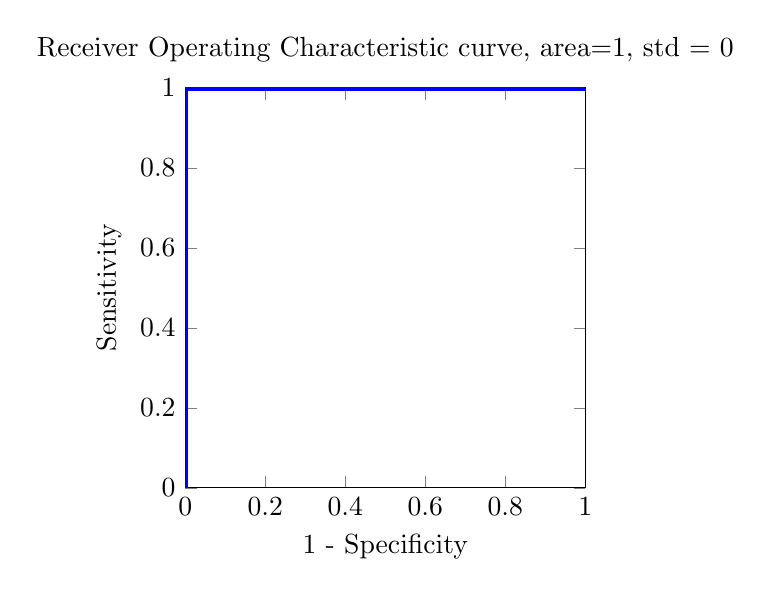
\begin{tikzpicture}

\begin{axis}[%
width=2.0in,
height=2.0in,
scale only axis,
xmin=0,
xmax=1,
xlabel={1 - Specificity},
ymin=0,
ymax=1,
ylabel={Sensitivity},
title={Receiver Operating Characteristic curve, area=1, std = 0}
]
\addplot [color=blue,solid,line width=2.0pt,forget plot]
  table[row sep=crcr]{%
0	0\\
0	0.0666666666666667\\
0	0.133333333333333\\
0	0.2\\
0	0.266666666666667\\
0	0.333333333333333\\
0	0.4\\
0	0.466666666666667\\
0	0.533333333333333\\
0	0.6\\
0	0.666666666666667\\
0	0.733333333333333\\
0	0.8\\
0	0.866666666666667\\
0	0.933333333333333\\
0	1\\
0.2	1\\
0.4	1\\
0.6	1\\
0.8	1\\
1	1\\
};
\end{axis}
\end{tikzpicture}%
\end{document}
\caption{ROC curve of an ideal classifier.}
\label{fig:roc}
\end{figure}


\subsection{Full complexity iris data set classification}
There is no reason not to subject least squares support vector machines to the full four dimensional classification problem as seen in figure~\ref{fig:originalIris}. An experiment is done where 30 of the 150 iris plant data points are set aside for validation. The remaining values serve as training data. Automatically trained linear and rbf-kernel svm did not miss-classify a single iris flower and got optimal roc-curves such as the one shown in figure~\ref{fig:roc}.